% Tex! = xelatex
\documentclass[fontset=windows]{ctexbook}
\usepackage{hyperref}
\usepackage{titletoc}
\usepackage{zhnumber}
\usepackage{fontawesome}
\usepackage{tikz}
\usepackage{ruby}
%\usepackage{coffeestains}
\renewcommand{\rubysep}{-1.3ex} %调整行间注与正文的距离
%\usepackage{emptypage} %不显示空白页页码
\usepackage{geometry}
\geometry{xetex,twoside,landscape,left=3cm,right=2cm,asymmetric=true,marginparwidth={0cm},marginparsep={15mm}}
\usepackage{xparse}

\defaultCJKfontfeatures{RawFeature={vertical:+vert:+vhal}}
\AtBeginShipout{%
  \global\setbox\AtBeginShipoutBox\vbox{%
    \special{pdf: put @thispage <</Rotate 90>>}%
    \box\AtBeginShipoutBox
  }%
}
\setCJKmainfont[FallBack={Source Han Serif TC}]{Source Han Serif SC}%在ctex中 [AutoFallback = true]属性不可用。
\punctstyle{plain}
%\xeCJKEditPunctStyle{plain}{optimize-kerning=false}
\newcommand*\CJKmovesymbol[1]{\raise.32em\hbox{#1}}
\newcommand*\CJKmovepunctsymbol[1]{\raise.6em\hb@xt@\z@{\hss#1}}
\newcommand*\CJKnopunctsymbol[1]{\setbox0=\hb@xt@\z@{\hss#1}\null}  %也不知道為什麼總之這樣可以把標點都消滅
 
\newcommand*\CJKmove{
  
  \xeCJKnobreakbetweenpuncts
  \let\CJKsymbol\CJKmovesymbol
  \let\CJKpunctsymbol\CJKsymbol
  %\let\CJKpunctsymbol\CJKmovepunctsymbol
  } %修正baseline


\AtBeginDocument{\CJKmove \sloppy}

\ExplSyntaxOn

\NewDocumentCommand{\readCIDfile}{m}
 {
  \readcid_file:n { #1 }
 }

\NewDocumentCommand{\CID}{m}
 {
  \use:c { CID#1 }
 }
\NewDocumentCommand{\UTF}{m}
 {
  \symbol { \int_from_hex:n { #1 } }
 }

\ior_new:N \g_readcid_file_stream

\cs_new_protected:Nn \readcid_file:n
 {
  \ior_open:Nn \g_readcid_file_stream { #1 }
  \ior_str_map_inline:Nn \g_readcid_file_stream
   {
    \__readcid_line:n { ##1 }
   }
 }


\cs_new_protected:Nn \__readcid_line:n
 {
  \__readcid_line_aux:w #1 \q_stop
 }

\cs_new_protected:Npn \__readcid_line_aux:w #1 ~ #2 \q_stop
 {
  \str_if_eq:nnF { #1 } { #2 }
   {
    \str_case_e:nnF { \str_range:nnn { #2 } { 1 } { 3 } }
     {
      {/un}{ \__readcid_def_uni:nn { #1 } { #2 } }
      {/Ja}{ \__readcid_def_japan:nn { #1 } { #2 } }
      {./n}{ }
     }
     { \__readcid_def:nn { #1 } { #2 } }
   }
 }

\cs_new_protected:Nn \__readcid_def:nn
 {
  \str_if_in:nnTF { #1 } { . }
   {
    \__readcid_def:w #1 - { #2 }
   }
   {
    \__readcid_def_do:nn { #1 } { #2 }
   }
 }
\cs_new_protected:Npn \__readcid_def:w #1..#2 - #3
 {
  \int_step_inline:nnn { #1 } { #2 }
   {
    \__readcid_def_do:nn { ##1 } { #3 }
   }
 }
\cs_new_protected:Nn \__readcid_def_do:nn
 {
  \cs_new:cpx {CID#1} { \UTF { #2 } }
 }

\cs_new_protected:Nn \__readcid_def_uni:nn
 {
  \str_if_in:nnTF { #1 } { . }
   {
    \__readcid_def_uni_multi:w #1 - { #2 }
   }
   {
    \__readcid_def_uni_do:nn { #1 } { #2 }
   }
 }
\cs_new_protected:Npn \__readcid_def_uni_multi:w #1..#2 - #3
 {
  \int_step_inline:nnn { #1 } { #2 }
   {
    \__readcid_def_uni_do:nn { ##1 } { #3 }
   }
 }
\cs_new_protected:Nn \__readcid_def_uni_do:nn
 {
  \cs_new:cpx {CID#1} { \UTF { \str_range:nnn { #2 } { 5 } { 8 } } }
 }

\cs_new_protected:Nn \__readcid_def_japan:nn
 {
  \str_if_in:nnTF { #1 } { . }
   {
    \__readcid_def_japan_multi:w #1 - { #2 }
   }
   {
    \__readcid_def_japan_do:nn { #1 } { #2 }
   }
 }
\cs_new_protected:Npn \__readcid_def_japan_multi:w #1..#2 - #3
 {
  \int_step_inline:nnn { #1 } { #2 }
   {
    \__readcid_def_japan_do:nn { ##1 } { #3 }
   }
 }
\cs_new_protected:Nn \__readcid_def_japan_do:nn
 {
  \cs_new:cpx {CID#1} { \CID { \__readcid_japan_strip:w #2 \q_stop } }
 }
\cs_new:Npn \__readcid_japan_strip:w #1.#2.#3 \q_stop { #2 }

\ExplSyntaxOff


\readCIDfile{/usr/local/texlive/2021/texmf-dist/fonts/cid/fontforge/Adobe-Japan1-6.cidmap} %texlive发行版本中的cidmap地址






%\usepackage{fontspec}

% \usepackage{fontspec}
% \usepackage{tabulary}
% \def\UTF#1{\char"#1}
% \def\CID#1{\XeTeXglyph#1}
%\usepackage{zxotf}
%\usepackage{CJKpunct}
%\usepackage{showframe}

%% 边注的宽度由长度\marginparwidth控制,与正文之间的水平距离由\marginparsep决定。
%% asymmetric参数控制左边距和右边距不会因翻页而互换。asymmetric=true表示不互换,以保证twoside模式下,头注边距的一致性。且为了页面上下对称,应满足 top = left - marginparwidth = right
\usepackage{indentfirst}
\usepackage{fancyhdr}
\usepackage{gezhu}
\expandafter\everywithgezhu\expandafter{\the\everywithgezhu}
  \everygezhu{\fontsize{11}{11}\selectfont \color{blue}}\setgezhuraise{-3pt}
  %\gezhuraggedture %%「」换为 ﹁﹂
\usepackage{marginnote}
\usepackage{endnotes}
\renewcommand{\notesname}{
\begin{flushleft}
  【尾注】
\end{flushleft}}
\makeatletter
\newskip\@endindent
\@endindent=1em
\long\def\@makeentext#1{\@setpar{\@@par\@tempdima \hsize
\advance\@tempdima-\@endindent
\parshape \@ne \@endindent \@tempdima}\par
\noindent \hbox to \z@{\hss\@theenmark\hspace{0.2em}}#1}
\renewcommand\theendnote{\myendnotestyle{\arabic{endnote}}}
\def\@makeenmark{\hbox{\textsuperscript{\@theenmark}}}%正文中脚注标签采取上标形式
\usepackage{pifont}
\newcommand\myendnotestyle[1]{\ifcase#1 \or \ding{192}\or \ding{193}\or
\ding{194}\or \ding{195}\or \ding{196}\or \ding{197}%
\or \ding{198}\or \ding{199}\or \ding{200}\or \ding{201}\else *\fi\relax}%数字单纯带圈,正常数字
\makeatother

% \makeatletter
% \let\shipout@temp=\shipout
% \def\shipout{\shipout@hook\shipout@temp}
% \def\shipout@hook{%
%   \setbox\@outputbox=\vbox to\pagegoal{\pageboxfronthook\unvbox\@outputbox\pageboxbackhook}}

% \newbox\linebox
% \def\eatlines{%
%   \setbox\linebox\lastbox
%   \ifvoid\linebox\else
%     \unskip\unpenalty
%     {\eatlines}%
%     \hbox{\lineboxfronthook\box\linebox\lineboxendhook}%
%   \fi}

% \newbox\@parbox
% \newbox\parsplit
% \newdimen\pageblank
% \AtBeginDocument{%
%   \everypar{%
%     \setbox\@parbox=\vbox\bgroup%或者\vtop
%     \everypar{}%
%     \def\par{\parboxinnerhook\@par\eatlines\egroup\parboxfronthook
%       \pageblank=\pagegoal
%       \advance\pageblank by-\pagetotal
%       \advance\pageblank by-1pt
%       \ifdim\ht\@parbox>\pageblank
%         \setbox\parsplit=\vsplit\@parbox to\pageblank
%         \vbox{\unvbox\parsplit}%
%         \pagebreakbackhook
%         \break
%         \pagebreakfronthook
%       \fi
%       \box\@parbox\parboxbackhook\@par}}}
% \def\parboxfronthook{\kern-\parindent\llap{\texttt{PAR FRONT}}}
% \def\parboxinnerhook{\texttt{PAR INNER}}
% \def\parboxbackhook{\rlap{\texttt{PAR BACK}}}
% \def\pagebreakfronthook{\llap{\texttt{PAGE BREAK FRONT}}}
% \def\pagebreakbackhook{\rlap{\texttt{PAGE BREAK BACK}}}
% \def\lineboxfronthook{\texttt{>>}}
% \def\lineboxendhook{\texttt{<<}}
% \def\pageboxfronthook{\ifdim\pagetotal<1\pagegoal{A}\fi}
% %\def\pageboxbackhook{B\ifdim\pagetotal<.5\pagegoal\vfill\hbox to\hsize{\hfill NULL\hfill}\vfill\fi}
% \def\pageboxbackhook{\quad}
% \makeatother

\xeCJKsetup{AutoFallBack=true} %启用AutoFallBack(本选项默认是false)
\usepackage{subfig,graphicx}
% \usepackage{varwidth} %% 提供 varwidth 环境
\ctexset{
chapter/name = {,},
chapter/format = \leavevmode\kern-18pt\LARGE\itshape,
chapter/fixskip = true,
chapter/beforeskip = 0pt,
chapter/afterskip = 12pt
}
% \newcommand\chaptertitleformat[1]{%% 以标题内容为参数
% \begin{varwidth}[t]{.7\linewidth}#1\end{varwidth}}
%\newcommand\chaptertitle[1]{\leavevmode\kern-36pt\raise0.0pt\hbox{\fontsize{18pt}{30}\selectfont{#1}}\kern0.1pt}


\usepackage{color,xcolor}
%\usepackage{setspace}

\makeatletter
%endnotes%
\def\enoteheading{\section*{\notesname
  \@mkboth{\MakeUppercase{\notesname}}{\MakeUppercase{\notesname}}}%
  \mbox{}\par\vskip-2.3\baselineskip\noindent\rule{.5\textwidth}{0.4pt}\par\vskip\baselineskip}
\makeatletter


\makeatletter 
% 删除宏包marginnote中的margintest命令在twoside模式下奇数偶数页的边注位置判断
\renewcommand*{\@mn@margintest}{%
  \expandafter\ifx\csname @mn@thispage\endcsname\@empty
    \gdef\@mn@atthispage{1}%
  \else\expandafter\ifnum \@mn@thispage=\value{mn@abspage}%
      \begingroup
        \@tempcnta\@mn@atthispage\advance\@tempcnta by \@ne
        \xdef\@mn@atthispage{\the\@tempcnta}%
      \endgroup
    \else
      \gdef\@mn@atthispage{1}%
    \fi
  \fi
  \xdef\@mn@thispage{\themn@abspage}%
  \let\@mn@currpage\relax
  \let\@mn@currxpos\relax
  \mn@savepos
  \protected@write\@auxout{\let\themn@abspage\relax}{%
    \string\newmarginnote{note.\@mn@thispage.\@mn@atthispage}{%
      {\themn@abspage}{\noexpand\number\mn@lastxpos sp}}%
  }%
  \expandafter\ifx\csname mn@note.\@mn@thispage.\@mn@atthispage\endcsname\relax
    \if@twoside
      \if@mn@verbose
        \PackageInfo{marginnote}{Suggest that margin
          note \@mn@thispage.\@mn@atthispage\space will be on\MessageBreak
          absolute page \themn@abspage.\MessageBreak
          This may be wrong}%
      \fi
      \ifodd\value{mn@abspage}\@tempswatrue\else\@tempswafalse\fi
    \else
      \if@mn@verbose
        \PackageInfo{marginnote}{right page because not two side mode}%
      \fi
      \@tempswatrue
    \fi
  \else
    \edef\@mn@currpage{\csname
      mn@note.\@mn@thispage.\@mn@atthispage\endcsname}%
    \edef\@mn@currxpos{\expandafter\@secondoftwo\@mn@currpage}%
    \ifx\@mn@currxpos\@empty\else
      \edef\@mn@currxpos{\the\dimexpr \@mn@currxpos -\hoffset\relax}%
      \begingroup\expandafter\expandafter\expandafter\endgroup
      \expandafter\ifx\csname pdfhorigin\endcsname\relax\else
        \begingroup\expandafter\expandafter\expandafter\endgroup
        \expandafter\ifx\csname pdfoutput\endcsname\relax
          \begingroup\expandafter\expandafter\expandafter\endgroup
          \expandafter\ifx\csname outputmode\endcsname\relax\else
            \ifnum \outputmode=1 %
              \edef\@mn@currxpos{\the\dimexpr \@mn@currxpos -\pdfhorigin
                +1in\relax}%
            \fi
          \fi
        \else
          \ifnum \pdfoutput=1 %
            \edef\@mn@currxpos{\the\dimexpr \@mn@currxpos -\pdfhorigin
              +1in\relax}%
          \fi
        \fi
      \fi
      \ifdefined\mn@pagewidth
        \@mn@if@RTL{%
          \PackageInfo{marginnote}{Margin note
            \@mn@thispage.\@mn@atthispage\space in RTL mode}%
          \edef\@mn@currxpos{%
            \the\dimexpr\mn@pagewidth-\@mn@currxpos\relax
          }%
        }{}%
      \fi
    \fi
    \edef\@mn@currpage{\expandafter\@firstoftwo\@mn@currpage}%
    \if@mn@verbose
      \PackageInfo{marginnote}{Margin note \@mn@thispage.\@mn@atthispage\space
        is on absolute page \@mn@currpage}%
    \fi
    % \if@twoside
    %   \ifodd\@mn@currpage\relax
    %     \@tempswatrue
    %     \if@twocolumn
    %       \ifdim \@mn@currxpos
    %              < \dimexpr\oddsidemargin+\columnwidth+\columnsep\relax
    %         \@tempswafalse
    %       \fi
    %     \fi
    %   \else
    %     \@tempswafalse
    %     \if@twocolumn
    %       \ifdim\@mn@currxpos>\dimexpr\evensidemargin+\columnwidth\relax
    %         \@tempswatrue
    %       \fi
    %     \fi
    %   \fi
    % \else
    %   \if@mn@verbose
    %     \PackageInfo{marginnote}{right page because not two side mode}%
    %   \fi
    %   \@tempswatrue
    %   \if@twocolumn
    %     \ifdim \@mn@currxpos
    %            < \dimexpr\oddsidemargin+\columnwidth+\columnsep\relax
    %       \@tempswafalse
    %     \fi
    %   \fi
    % \fi
  \fi
}
\renewcommand{\footnotesize}{\normalsize}
\makeatletter

\makeatletter
% 设置宏包fancyhdr中的fancyplain的页眉分割线宽度为0pt(即不显示分割线)
\def\headrulewidth{0pt}%
\makeatletter

\let\oldmarginnote\marginnote
% \renewcommand\marginpar[1]{\-\oldmarginpar[\raggedleft\footnotesize #1]%
% {\raggedright\color{red}\footnotesize #1}} % 
% \marginparsep = 10pt %与正文间隔10pt
\renewcommand\marginnote[1]{\-\oldmarginnote[\raggedright\color{red}\footnotesize #1]%
{\raggedright\color{red}\footnotesize #1}} % 注释文字用红色footnote 大小

%\renewcommand{\headrulewidth}{0pt}
%\renewcommand{\chaptermark}[1]{\markright{#1}}

\renewcommand{\rightmark}{\@title}

\fancypagestyle{fancyplain}{
\fancyhf{}
\fancyhead[EL]{\leavevmode\kern18em\raise0.0pt\hbox{\fontsize{10pt}{9}\selectfont{~}}\kern.1pt}
\fancyhead[ER]{\thepage}
\fancyfoot[OL]{{~~~~~~~~~~~~~~~~~~~~~~~~~~~~~~~~~~~~~~~~~~~~~~~~~~}\rightmark}
\fancyfoot[OR]{\thepage}
}

\fancypagestyle{fancyplain2}{
\fancyhf{}
\fancyhead[EL]{\leavevmode\kern18em\raise0.0pt\hbox{\fontsize{10pt}{9}\selectfont{后记}}\kern.1pt}
\fancyhead[ER]{\thepage}
\fancyfoot[OL]{{~~~~~~~~~~~~~~~~~~~~~~~~~~~~~~~~~~~~~~~~~~~~~~~~~~}\rightmark}
\fancyfoot[OR]{\thepage}
}
%\newskip\sepskip


\fancypagestyle{maintext}{
\fancyhf{}
\fancyhead[EL]{{~~~~~~~~~~~~~~~~~~~~~~~~~~~~~~~~~~~~~~~~~~~~~~~~~~}\leftmark}
\fancyhead[ER]{\thepage}
\fancyfoot[OL]{{~}\rightmark}
\fancyfoot[OC]{{~~~~~~~~~~~~~~~~~~~~~~~~~~~~~~~~~~~~~~~~~~~~~~~~~~~~~~~~~~~~~~~~~~~~~~~~~~~~~~~~~~~~~~~~~~~~~~}\thepage}
}

\fancypagestyle{fancy}{
\fancyhf{}
\fancyhead[EL]{{~~~~~~~~~~~~~~~~~~~~~~~~~~~~~~~~~~~~~~~~~~~~~~~~~~}\leftmark}
\fancyhead[ER]{\thepage}
\fancyfoot[OL]{{~~~~~~~~~~~~~~~~~~~~~~~~~~~~~~~~~~~~~~~~~~~~~~~~~~}\rightmark}
\fancyfoot[OR]{\thepage}
}

\fancypagestyle{plain}{}

%


%\setCJKmainfont{A-OTF-SeiKaiCB1Pr5-Regular.otf} %[BoldFont = SimHei , ItalicFont = KaiTi]



\pagenumbering{chinese}
%\dottedcontents{chapter}[0em]{\normalsize}{4.0em}{6pt}
\titlecontents{chapter}[1cm]{\fontsize{14pt}%
{\baselineskip}\selectfont}{\hspace*{3em}\contentslabel{4em}\ }%
{}{\titlerule*[0.5pc]%
{$\cdot$}\contentspage\hspace*{1cm}}%
%titletoc宏包,它与titlesec宏包的文档写在同一个pdf文件中。

%\dottecontents{section}[left]{above-code}{label-width}{leader-width}
%\titlecontents{section}[left]{above-code}{numbered-entry-format}{numberless-entry-format}{filler-page-format}[below-code]

%各参数的含义如下所示:
%section:目录对象,可以填 chapter 、section,或者figure、table。
%left:目录对象左侧到左页边区的距离,一般必选。
%above-code:格式调整命令,可以包含垂直对象,也可以用\contentslabel,即指定本级别目录标签箱子的宽度。
%label-width:标签宽。
%leader-width:填充符号宽,默认的填充符号是圆点。
%numbered-entry-format:如果有标签,表示在目录文本前输入的格式。
%numberless-entry-format:没有标签时输入的格式。
%filler-page-format:填充格式,一般借助titlesec中的\titlerule*[width]{text}命令。
%below-code:在entry之后输入的格式,比如垂直空距。

\setlength{\parindent}{0pt} 
\setlength{\headheight}{15.7301pt}
\linespread{1.1} %ctex定义的行距倍数
\setlength{\parskip}{0pt}

\title{长短经校注}
\author{唐\quad 赵蕤}
\date{}
%\authorfn{庚辰本}

%%%%%%	自定義的公式 示例

\newcommand\sampleEq{%
  \left(\int_0^\infty \frac{\sin x}{\sqrt{x}}dx\right)^2
  = \sum_{k=0}^\infty \frac{(2k)!}{2^{2k}(k!)^2} \frac{1}{2k+1}
  = \prod_{k=1}^\infty \frac{4k^2}{4k^2-1}
  \neq \frac{\pi}{2015}}

%%%%%%	自定義的公式 示例(結束)
\usepackage[pages=some, scale=1,,angle=90]{background}

%\usepackage{ifthen}
%\AddEverypageHook{%
% \ifthenelse{\isodd{\value{page}}}%
% {
  \backgroundsetup{
  %angle=90,
  %position={0,0},
  contents={%
  \begin{tikzpicture}[color={red}, remember picture, overlay,opacity=1]
    \draw[-,line width=4pt] (-6.975,6.9)--(8.875,6.9);%画外框
    \draw[-,line width=4pt] (-6.975,-12.3)--(8.875,-12.3);
    \draw[-,line width=4pt] (-6.9,6.83)--(-6.9,-12.23);
    \draw[-,line width=4pt] (8.8,6.83)--(8.8,-12.23);
    %
    \draw[-,line width=1pt] (-6.7,6.7)--(8.6,6.7);%画内框
    \draw[-,line width=1pt] (-6.7,-12.1)--(8.6,-12.1);
    \draw[-,line width=1pt] (-6.7,6.7)--(-6.7,-12.1);
    \draw[-,line width=1pt] (8.6,6.7)--(8.6,-12.1);
    %
    \draw[->] (-5.52307692307692,6.7)--(-5.52307692307692,-12.1);
\draw[->] (-4.34615384615385,6.7)--(-4.34615384615385,-12.1);
\draw[->] (-3.16923076923077,6.7)--(-3.16923076923077,-12.1);
\draw[->] (-1.99230769230769,6.7)--(-1.99230769230769,-12.1);
\draw[->] (-0.815384615384615,6.7)--(-0.815384615384615,-12.1);
\draw[->] (0.361538461538462,6.7)--(0.361538461538462,-12.1);
\draw[->] (1.53846153846154,6.7)--(1.53846153846154,-12.1);
\draw[->] (2.71538461538462,6.7)--(2.71538461538462,-12.1);
\draw[->] (3.89230769230769,6.7)--(3.89230769230769,-12.1);
\draw[->] (5.06923076923077,6.7)--(5.06923076923077,-12.1);
\draw[->] (6.24615384615385,6.7)--(6.24615384615385,-12.1);
\draw[->] (7.42307692307693,6.7)--(7.42307692307693,-12.1);
  \end{tikzpicture}
  }
}%
%}
% {
%   \backgroundsetup{
%   %angle=90,
%   %position={0,0},
%   contents={%
%   \begin{tikzpicture}[color={red}, remember picture, overlay]
%     \draw[-,line width=4pt] (-7.175,6.9)--(8.475,6.9);%画外框
%     \draw[-,line width=4pt] (-7.175,-12.3)--(8.475,-12.3);
%     \draw[-,line width=4pt] (-7.1,6.83)--(-7.1,-12.23);
%     \draw[-,line width=4pt] (8.4,6.83)--(8.4,-12.23);
%     %
%     \draw[-,line width=1pt] (-6.9,6.7)--(8.2,6.7);%画内框
%     \draw[-,line width=1pt] (-6.9,-12.1)--(8.2,-12.1);
%     \draw[-,line width=1pt] (-6.9,6.7)--(-6.9,-12.1);
%     \draw[-,line width=1pt] (8.2,6.7)--(8.2,-12.1);
%     %
%     \draw[-,line width=1pt] (-5.73846153846154,6.7)--(-5.73846153846154,-12.1);
%     \draw[-,line width=1pt] (-4.57692307692308,6.7)--(-4.57692307692308,-12.1);
%     \draw[-,line width=1pt] (-3.41538461538462,6.7)--(-3.41538461538462,-12.1);
%     \draw[-,line width=1pt] (-2.25384615384616,6.7)--(-2.25384615384616,-12.1);
%     \draw[-,line width=1pt] (-1.09230769230769,6.7)--(-1.09230769230769,-12.1);
%     \draw[-,line width=1pt] (0.0692307692307672,6.7)--(0.0692307692307672,-12.1);
%     \draw[-,line width=1pt] (1.23076923076923,6.7)--(1.23076923076923,-12.1);
%     \draw[-,line width=1pt] (2.39230769230769,6.7)--(2.39230769230769,-12.1);
%     \draw[-,line width=1pt] (3.55384615384615,6.7)--(3.55384615384615,-12.1);
%     \draw[-,line width=1pt] (4.71538461538461,6.7)--(4.71538461538461,-12.1);
%     \draw[-,line width=1pt] (5.87692307692307,6.7)--(5.87692307692307,-12.1);
%     \draw[-,line width=1pt] (7.03846153846153,6.7)--(7.03846153846153,-12.1);          
%   \end{tikzpicture}
%   }
%   }%
% }
  %\BgMaterial
  %\BgThispage
 %}

\begin{document}
\begin{titlepage}
  \pagestyle{empty} %封面不显示页码和页眉页脚
  \vspace*{10mm}
  \noindent{\Huge \@title}
  \vfill
  \begin{flushright}
    {\Large \@author}
  \end{flushright}
\end{titlepage}

\pagestyle{fancyplain}
\setcounter{page}{1}
\fontsize{18}{30}\selectfont
\begin{withgezhu}
  \chapter*{前言}
《长短经》是唐代西蜀赵蕤所著。据赵蕤自序,原为十卷六十三篇。后来第十卷《阴谋》缺失。今存九卷,计《文上》、《文中》、《文下》、《霸纪上》、《霸纪中》、《霸纪下》、《权议》、《杂说》和《兵权》,共六十四篇。

现存《长短经》最早的版本为南宋绍兴(1131-1162)年间刊本,清乾隆间修《四库全书》,用的就是这一版本。清代以来,《长短经》的重要版本还有《读画斋丛书》本(《丛书集成初编》本即据此排印)等。
国内出版的版本主要有周斌《<长短经>校证与研究》(巴蜀书社2003年版)、刘国建注译本《长短经》(长春出版社2001年版),以及张兆凯等注译本《长短经》(岳麓书社1999年版)等。



\newpage
\chapter*{自序}
\begin{flushright}
    赵蕤 
\end{flushright}
匠成舆者,忧人不贵;作箭者,恐人不伤。彼岂有爱憎哉?实技业驱之然耳。是知当代之士、驰骛之曹,书读纵横,则思诸侯之变;艺长奇正,则念风尘之会。此亦向时之论,必然之理矣。故先师孔子深探其本、忧其末,遂作《春秋》,大乎王道;制《孝经》,美乎德行。防萌杜渐,预有所抑。斯圣人制作之本意也。

然作法于理,其弊必乱。若至于乱,将焉救之?是以御世理人,罕闻沿袭。三代不同礼,五霸不同法。非其相反,盖以救弊也。是故国容一致,而忠文之道必殊;圣哲同风,而皇王之名或异。岂非随时投教沿乎此,因物成务牵乎彼?沿乎此者,醇薄继于所遭;牵乎彼者,王霸存于所遇。故古之理者,其政有三:王者之政化之;霸者之政威之;强国之政胁之。各有所施,不可易也。管子曰:“圣人能辅时不能违时。智者善谋,不如当时。”邹子曰:“政教文质,所以匡救也。当时则用之,过则舍之。”由此观之,当霸者之朝而行王者之化,则悖矣。当强国之世而行霸者之威,则乖矣。若时逢狙诈,正道陵夷,欲宪章先王,广陈德化,是犹待越客以拯溺,白大人以救火。善则善矣,岂所谓通于时变欤?

夫霸者,驳道也。盖白黑杂合,不纯用德焉。期于有成,不问所以;论于大体,不守小节。虽称仁引义不及三王,扶颠定倾,其归一揆。恐儒者溺于所闻,不知王霸殊略,故叙以长短术,以经论通变者,并立题目总六十有三篇,合为十卷,名曰《反经》。大旨在乎宁固根蒂,革易时弊,兴亡治乱。具载诸篇,为沿袭之远图,作经济之至道,非欲矫世夸欲,希声慕名。辄露见闻,逗机来哲。凡厥有位,幸望详焉。


\end{withgezhu}



\clearpage
\pagestyle{plain}
\setcounter{page}{1}
%\newpage\NoBgThispage
\tableofcontents


\newgeometry{twoside,left=8cm,right=2cm,asymmetric=true,marginparwidth={4.5cm},marginparsep={15mm}}

%\newpage
%\clearpage
\pagestyle{maintext}
\renewcommand\baselinestretch{1.1}\selectfont


%%%%%%%%%%%%测试页面Hook
%\def\pageboxfronthook{\hbox{\fontsize{18pt}{30}\selectfont{匚}}\vfill \hbox to\hsize{\hfill NULL\hfill}\vfill}

\begin{withgezhu}
  \setcounter{page}{1}

  %\input{text/bodytext1.tex}
  %\newpage
  \AddEverypageHook{%此后每页都添加网格
  \BgMaterial
  % \coffeestainA{0.9}{0.85}{-25}{5cm}{1.3cm}
  % \coffeestainD{0.4}{0.5}{90}{3 cm}{4 cm}
  }

  \chapter{大体}%
臣闻老子曰:﹁以正理国,以奇用兵,以无事取天下。﹂荀卿曰:﹁人主者,以官人为能者也;匹夫者,以自能为能者也。﹂傅子曰:﹁士大夫分职而听,诸侯之君分土而守,三公总方而议,则天子拱己而正矣。﹂何以明其然耶?当尧之时,舜为司徒,契为司马,禹为司空,后稷为田畴,夔为乐正,倕为工师,伯夷为秩宗,皋陶为理官,益掌驱禽。尧不能为一焉,奚以为君,而九子者为臣,其故何也?尧知九赋之事,使九子各授其事,皆胜其任以成九功。尧遂乘成功以王天下。\\
汉高帝曰:﹁夫运筹策于帏幄之中,决胜于千里之外,吾不如子房;镇国家,抚百姓,给饷馈,不绝粮道,吾不如萧何;连百万之军,战必胜,攻必取,吾不如韩信。三人者,皆人杰也。吾能用之,此吾所以有天下也。﹂
\gezhu{《人物志》曰:﹁夫一官之任,以一味协五味;一国之政,以无味和五味。故臣以自任为能,君以能用人为能;臣以能言为能,君以能听为能;臣以能行为能,君以能赏罚为能。所以不同,故能君众能也。﹂}\\
故曰:知人者,王道也;知事者,臣道也。无形者,物之君也;无端者,事之本也。鼓不预五音,而为五音主;有道者,不为五官之事,而为理事之主。君守其道,官知其事,有自来矣。\\
先王知其如此也,故用非其有,如己有之,通乎君道者也。
\gezhu{议曰:《淮南子》云:﹁巧匠为宫室,为圆必以规,为方必以矩,为平直必以准绳。功已就矣,而不知规矩准绳,而赏巧匠。宫室已成,不知巧匠,而皆曰某君某王之宫室也。﹂\\
孙卿曰:﹁夫人主欲得善射中微,则莫若使羿;欲得善御致远,则莫若使王良;欲得调一天下,则莫若聪明君子矣。其用智甚简,其为事不劳,而功名甚大。﹂此能用非其有,如己有者也。}\\
人主不通主道者,则不然。自为之,则不能任贤;不能任贤,则贤者恶之。此功名之所以伤,国家之所以危。
\gezhu{议曰:﹁《申子》云:﹁君知其道也,臣知其事也。十言十当,百言百当者,人臣之事也,非人君之道也。﹂《尸子》云:﹁人臣者,以进贤为功也;君者,以用贤为功也。﹂贾谊云:﹁臣闻圣主言问其臣,而不自造事,故使人臣得必尽其愚忠,惟陛下财幸。﹂由是言之,夫君不能司契委任而妒贤恶能,取败之道也。}\\
汤武日而尽有夏商之财,以其地封,而天下莫敢不悦服;以其财赏,而天下皆竞劝,通乎用非其有也。
\gezhu{议曰:孙卿云:﹁修礼者王,为政者强,取人者安,聚敛者亡。故王者富人,霸者富士,仅存之国富大夫,亡国富筐箧、实府库。是谓上溢下漏。﹂又曰:﹁天子不言多少,诸侯不言利害,大夫不言得失。﹂\\
昔者周厉王好利,近荣公,芮良夫谏曰:﹁王室其将卑乎?荣公好专利而不知大难。夫利,百物之所生也,天地之所载也;而有专之,其害多矣。天地百物皆将取焉,何可专也!所利甚多而不备大难,以是教王,其能久乎?﹂后厉王果败。\\
魏文侯御廪灾,素服避正殿,群臣皆哭。公子成父趋入贺曰:﹁臣闻天子藏于四海,诸侯藏于境内。非其所藏,不有火灾,必有人患。幸无人患,不亦善乎!﹂孔子曰:﹁百姓足,君孰不足?﹂周谚有言曰:﹁囊漏储中。﹂由此言之,夫圣王以其地封,以其财赏,不与人争利,乃能通于王道,是用非其有者也。}\\
故称:设官分职,君之体也;委任责成,君之体也;好谋无倦,君之体也;宽以得众,君之体也;含垢藏疾,君之体也。君有君人之体,其臣畏而爱之,此帝王所以成业也。
%
%
\chapter{任长}%
臣闻料才核能,治世之要。自非圣人,谁能兼兹百行、备贯众理乎?故舜合群司,随才授位;汉述功臣,三杰异称。况非此俦,而可备责耶?
\gezhu{《人物志》曰:夫刚略之人,不能理微,故论其大体,则宏略而高远;历纤理微,则宕往而疏越。亢厉之人,不能回挠,其论法直,则括据而公正;说变通,则否戾而不入。宽恕之人,不能速捷,论仁义,则宏详而长雅;趋时务,则迟后而不及。好奇之人,横逆而求异,造权谲,则倜傥而瑰壮;案清道,则诡常而恢迂。\\
又曰:王化之政,宜于统大,以之理小则迂;策术之政,宜于理难,以之理平则无奇;矫亢之政,宜于治侈,以之治弊则残;公刻之政,宜于纠奸,以之治边则失其众;威猛之政,宜于讨乱,以之治善则暴;伎俩之政,宜于治富,以之治贫则劳而下困。此已上皆偏材也。}\\
昔伊尹之兴土工也,强脊者使之负土,眇者使之推,伛者使之涂,各有所宜,而人性齐矣。管仲曰:﹁升降揖让,进退闲习,臣不如隰朋,请立以为大行;辟土聚粟,尽地之利,臣不如宁戚,请立以为司田;平原广牧,车不结辙,士不旋踵,鼓之而三军之士视死如归,臣不如王子城父,请立以为大司马;决狱折中,不杀不辜,不诬不罪,臣不如宾胥无,请立以为大理;犯君颜色,进谏必忠,不避死亡,不挠富贵,臣不如东郭牙,请立以为大谏。君若欲治国强兵,则五子者存焉;若欲霸王,则夷吾在此。﹂\\
黄石公曰:﹁使智,使勇,使贪,使愚。智者乐立其功,勇者好行其志,贪者决取其利,愚者不爱其死。因其至情而用之,此军之微权也。﹂\\
《淮南子》曰:﹁天下之物莫凶于溪毒\gezhu{附子也},然而良医橐而藏之,有所用也。麋之上山也,大章不能企;及其下也,牧竖能追之。才有修短也。胡人便于马,越人便于舟。异形殊类,易事则悖矣。﹂\\
魏武诏曰:﹁进取之士,未必能有行。有行之士,未必能进取。陈平岂笃行,苏秦岂守信耶?而陈平定汉业、苏秦济弱燕者,任其长也。﹂\\
由此观之,使韩信下帏,仲舒当戎,于公驰说,陆贾听讼,必无曩时之勋,而显今日之名也。故任长之道,不可不察。
\gezhu{议曰:魏·桓范云:﹁帝王用人,度世授才。争夺之时,书策为先。分定之后,忠义为首。故晋文行咎犯之计而赏雍季之言,高祖用陈平之智而托后于周勃。﹂古语云:﹁守文之代,德高者位尊;仓卒之时,功多者赏厚。﹂诸葛亮曰:﹁老子长于养性,不可以临危难;商鞅长于理法,不可以从教化;苏、张长于驰辞,不可以结盟誓;白起长于攻取,不可以广众;子胥长于图敌,不可以谋身;尾生长于守信,不可以应变;王嘉长于遇明君,不可以事暗主;许子将长于明臧否,不可以养人物。﹂此任长之术者也。}\\%
%
\chapter{品目}%
夫天下重器,王者大统,莫不劳聪明于品材,获安逸于任使。故孔子曰:﹁人有五仪:有庸人,有士人,有君子,有圣,有贤。审此五者,则治道毕矣。﹂\\
所谓庸人者,心不存慎终之规,口不吐训格之言\gezhu{格,法};不择贤以托身,不力行以自定;见小暗大而不知所务,从物如流而不知所执。此则庸人也。\\
所谓士人者,心有所定,计有所守。虽不能尽道术之本,必有率也\gezhu{率,犹述也};虽不能遍百善之美,必有处也。是故智不务多,务审其所知;言不务多,务审其所谓\gezhu{所谓,言之要也};行不务多,务审其所由。智既知之,言既得之\gezhu{得其要也},行既由之,则若性命形骸之不可易也。富贵不足以益,贫贱不足以损,此则士人也。\\
所谓君子者,言必忠信而心不忌\gezhu{忌,怨害也},仁义在身而色不伐,思虑通明而辞不专,笃行信道,自强不息,油然若将可越而终不可及者。此君子也。\gezhu{油然,不进之貌也。越,过也。孙卿曰:﹁夫君子能为可贵,不能使人必贵己;能为可信,不能使人必信己;能为可用,不能使人必用己。故君子耻不修,不耻见污;耻不信,不耻不见信;耻不能,不耻不见用。不诱于誉,不怨于诽,率道而行,端然正己,谓之君子也。﹂}\\
所谓贤者,德不逾闲\gezhu{闲,法也},行中规绳,言足法于天下而不伤其身\gezhu{言满天下,无口过也},道足化于百姓而不伤于本\gezhu{本亦身也},富则天下无菀财\gezhu{菀,积},施则天下不病贫。此则贤者也。\\
所谓圣者,德合天地,变通无方,究万事之终始,协庶品之自然,敷其大道而遂成情性,明并日月,化行若神,下民不知其德,睹者不识其邻\gezhu{邻,以喻界畔也}。此圣者也。
\gezhu{《庄子》曰:﹁刻意尚行,离世异俗,高论怨诽,为亢而已矣:此山谷之士,非世之人,枯槁赴渊者之所好也。语仁义忠信,恭俭推让,为修而已矣:此平世之士,教诲之人也,游居博学者之所好也。语大功,立大名,礼君臣,正上下,为治而已矣:此朝廷之士,尊主强国之人也,致功兼并者之所好也。就薮泽,处闲旷,钓鱼闲处,无为而已矣:此江海之士,避世之人也,闲暇者之所好也。吹呴呼吸,吐故纳新,熊经鸟伸,为寿而已矣:此导引之士,养形之人,彭祖寿考者之所好也。若夫不刻意而高,无仁义而修,无功名而治,无江海而闲,不导引而寿,无不忘也,无不有也。淡然无极而众美从之,此天地之道,圣人之德也。﹂}\\
《钤经》曰:﹁德足以怀远,信足以一异,识足以鉴古,才足以冠世,此则人之英也;法足以成教,行足以修义,仁足以得众,明足以照下,此则人之俊也;身足以为仪表,智足以决嫌疑,操足以厉贪鄙,信足以怀殊俗,此则人之豪也;守节而无挠,处义而不怒,见嫌不苟免,见利不苟得,此则人之杰也。﹂
\gezhu{《人物志》曰:﹁德行高妙,容止可法,是谓清节,延陵、晏婴是也。思信道化,策谋奇妙,是谓术家,范蠡、张良是也。其德足以厉风俗,其法足以正天下,其术足以谋庙胜,是谓国体,伊尹、吕望是也。其德足以率一国,其法足以正乡邑,其术足以权事宜,是谓器能,子产、西门豹是也。\\
清节之流,不能宏恕,好尚讥诃,分别是非,是谓臧否,子夏之徒是也。法家之流,不能创思图远,而能受一官之任,错意施巧,是为伎俩,张敝、赵广汉是也。术家之流,不能创制垂则,而能遭变用权;权智有余,公正不足,是谓智意,陈平、韩安国是也。能属文著述,是谓文章,司马迁、班固是也。能传圣人之业,而不能干事施政,是谓儒学,毛公、贯公是也。辩不入道,而应对资给,是谓口辩,乐毅、曹丘生是也。胆力绝众,材略过人,是谓骁雄,白起、韩信是也。﹂}\\
《家语》曰:﹁昔者明王必尽知天下良士之名,既知其名,又知其实,然后用天下之爵以尊之,则天下理也。﹂此之谓矣。


\chapter{量才}%
夫人才能参差,大小不同,犹升不可以盛斛,满则弃矣。非其人而使之,安得不殆乎?\gezhu{傅子曰:﹁凡品才有九:一曰德行,以立道本;二曰理才,以研事机;三曰政才,以经治体;四曰学才,以综典文;五曰武才,以御军旅;六曰农才,以教耕稼;七曰工才,以作器用;八曰商才,以兴国利;九曰辩才,以长讽议。﹂此量才者也。}\\
故伊尹曰:﹁智通于大道,应变而不穷,辩于万物之情,其言足以调阴阳、正四时、节风雨。如是者,举以为三公。﹂故三公之事常在于道。
\gezhu{汉文帝问陈平曰:﹁君所主何事?﹂对曰:﹁陛下不知臣驽下,使臣待罪宰相。宰相者,上佐天子,燮理阴阳,下遂万物之宜,外镇抚四夷,内亲附百姓,使公卿大夫各得其职。﹂上曰:﹁善!﹂\\
汉魏相书曰:﹁臣闻《易》曰:‘天地以顺动,故日月不过、四时不忒;圣人以顺动,则刑罚清而人服。’天地变化,必由阴阳。阴阳之分,以日月为纪。各有常职,不得相干。明主谨于尊天,慎于养人。故立羲和之官,以乘四时,敬授人事。君动静以道,奉顺阴阳,则日月光明,风雨时节,寒暑调和。三者得叙,则灾害不生,人不夭疾,衣食有余矣。此燮理阴阳之大体也。﹂事具〈洪范〉篇。}\\
不失四时,通于地利,能通不通,能利不利,如是者,举以为九卿。故九卿之事常在于德。\\
通于人事,行犹举绳,通于关梁,实于府库,如是者,举以为大夫。故大夫之事常在于仁。\gezhu{蜀丞相诸葛亮主簿杨颙曰:﹁坐而论道,谓之三公;作而行之,谓之卿大夫。﹂}\\
忠正强谏而无有奸诈,去私立公而言有法度,如是者,举以为列士。故列士之事常在于义也。故道德仁义定而天下正。\gezhu{《人物志》曰:﹁清节之德,师氏之任也;法家之材,司寇之任也;术家之材,三孤之任也;臧否之材,师氏之佐也;伎俩之材,司空之任也;儒学之材,保氏之任也;文章之材,国史之任也;骁雄之材,将帅之任也。﹂}\\
太公曰:﹁多言多语,恶口恶舌,终日言恶,寝卧不绝,为众所憎,为人所疾。此可使要遮闾巷,察奸伺祸。权数好事,夜卧早起,虽剧不悔,此妻子之将也。先语察事,劝而与食,实长希言,财物平均,此十人之将也。忉忉截截,垂意肃肃,不用谏言,数行刑戮,刑必见血,不避亲戚,此百人之将也。讼辩好胜,嫉贼侵凌,斥人以刑,欲整一众,此千人之将也。外貌怍怍,言语时出,知人饥饱,习人剧易,此万人之将也。战战栗栗,日慎一日,近贤进谋,使人知节,言语不慢,忠心诚毕,此十万人之将也\gezhu{《经》曰:﹁夫将虽以详重为贵,而不可有不决之疑;虽以博访为能,而不欲有多端之惑。﹂此论将之妙也。}。温良实长,用心无两;见贤进之,行法不枉,此百万人之将也。勋勋纷纷,邻国皆闻,出入豪居,百姓所亲,诚信缓大,明于领世,能效成事,又能救败,上知天文,下知地理,四海之内,皆如妻子,此英雄之率,乃天下之主也。﹂
\gezhu{《人物志》曰:﹁聪明秀出,谓之英;胆力过人,谓之雄。此其大体之别名也。夫聪明者,英之分也,不得雄之胆则说不行;胆力者,雄之分也,不得英之智则事不立。若聪能谋始,而明不见机,可以坐论而不可以处事;若聪能谋始,明能见机,而勇不能行,可以循常而不可以虑变;若力能过人,而勇不能行,可以为力人,未可以为先登;力能过人,勇能行之,而智不能料事,可以为先登,未足以为将帅。必聪能谋始,明能见机,胆能决之,然后乃可以为英,张良是也。气力过人,勇能行之,智足料事,然后乃可以为雄,韩信是也。若一人之身兼有英雄,则能长世,高祖、项羽是也。﹂}\\
《经》曰:﹁智如源泉,行可以为表仪者,人师也;智可以砥砺,行可以为辅警者,人友也;据法守职而不敢为非者,人吏也;当前快意,一呼再诺者,人隶也。故上主以师为佐,中主以友为佐,下主以吏为佐,危亡之主以隶为佐。﹂欲观其亡,必由其下。\\
故同明者相见,同听者相闻,同志者相从,非贤者莫能用贤。故辅佐左右所欲任使者,存亡之机,得失之要。\\
孙武曰:﹁主孰有道?
\gezhu{昔汉王见围荥阳,谓陈平曰:﹁天下纷纷,何时定乎?﹂平曰:﹁项王为人,恭敬爱人;士之廉节好礼者,多归之。至于行功赏爵,邑重之士,亦以此不附。今大王慢人少礼;士之顽钝嗜利无耻者,亦多归汉。诚宜各去两短,集其两长,天下指麾不足定也。﹂\\
魏太祖谓郭嘉曰:﹁袁本初地广兵强,吾欲讨之,力不能敌,何如?﹂嘉对曰:﹁刘、项之不敌,公所知也。汉祖惟智胜,项羽虽强,终为所擒。嘉窃料之,绍有十败,公有十胜,虽兵强,无能为也。\\
绍繁礼多仪,公体任自然,此道胜,一也。\\
绍以逆动,公以奉顺,以率天下,此义胜,二也。\\
汉末政失于宽,绍以宽济,故不慑;公纠之以猛,而上下知制,此治胜,三也。\\
绍外宽内忌,用人而旋疑之,所任唯亲戚子弟耳;公外简易而内机明,用人无疑,唯才能所宜,不问远近,此度胜,四也。\\
绍多计少决,失在事后;公策得辄行,应变无穷,此谋胜,五也。\\
绍因累世之资,高议揖让,以收名誉,士之好言饰外者多归之;公至心待人,推诚而行之,不为虚美,以俭率下,与有功者无所吝,士之忠正远见而有实者皆愿为用,此德胜,六也。\\
绍见人饥寒,恤念之情,形于颜色,其所不见,虑或不及,所谓妇人之仁耳;公于目前小事,时有所忽,至于大事,与四海相接,恩之所加,皆过其望,虽所不见,虑之所周,无不济也,此仁胜,七也。\\
绍以大臣争权,谗言惑乱;公御下以道,浸润不行,此明胜,八也。\\
绍是非不可知;公所是:进之以礼;所不是,正之以法,此文胜,九也。\\
绍好为虚势,不知兵要;公以少克众,用兵如神,军人恃之,敌人畏之,此武胜,十也。﹂\\
曹公曰:﹁吾知之,绍为人志大而智小,色厉而胆薄,忌克而少威,兵多而分画不明,将骄而政令不一,土地虽广,粮食虽丰,适所以为吾奉也。﹂\\
杨阜曰:﹁袁公宽而不断,好谋而少决。不断则无威,少决则后事。今虽强,终为所擒。曹公有雄才远略,决机无疑,法一而兵精,必能济大事也。﹂}\\
将孰有能?
\gezhu{袁绍率大众攻许,孔融谓荀彧曰:﹁袁绍地广兵强,田丰、许攸,智计之士,为其谋;审配、逢纪,尽忠之臣,任其事;颜良、文丑,勇冠三军,统其兵。殆难克乎?﹂彧曰:﹁绍兵虽多,而法令不整。田丰刚而犯上,许攸贪而不治,审配专而无谋,逢纪果而自用。此二人留,知后事。许攸贪而犯法,必不能纵,不纵必为变。颜良、文丑,一夫之勇耳,可一战而擒也。﹂后许攸贪不奉法,审配收其妻子,攸怒,奔曹公。又颜良临阵授首,田丰以谏死。皆如彧所料也。}\\
吾以此知胜之谓矣。
%
%
\chapter{知人}%
臣闻主将之法,务览英雄之心。然人未易知,知人未易。汉光武,聪听之主也,谬于庞萌;曹孟德,知人之哲也,弊于张邈。何则?夫物类者,世之所惑乱也。故曰:狙者类智而非智也,\gezhu{狙,音自舒反。慢也。}愚者类君子而非君子也,戆者类勇而非勇也。亡国之主似智,亡国之臣似忠,幽莠之幼似禾,骊牛之黄似虎,白骨疑象,碔砆类玉。此皆似是而非也。
\gezhu{《人物志》曰:﹁轻诺似烈而寡信,多易似能而无效,进锐似精而去速,诃者似察而事烦,诈施似惠而无终,面从似忠而退违。此似是而非者也。亦有似非而是者:有大权似奸而有功,大智似愚而内明,博爱似虚而实厚,正言似讦而情忠。非天下之至精,孰能得其实也?﹂}\\
孔子曰:﹁凡人心险于山川,难知于天。天犹有春秋冬夏、旦暮之期,人者厚貌深情,故有貌愿而益,有长若不肖\gezhu{长,音竹两反。},有顺懁而达,有坚而缦,有缓而焊\gezhu{音汗}。﹂\\
太公曰:﹁士有严而不肖者,有温良而为盗者,有外貌恭敬、中心欺慢者,有精精而无情者,有威威而无成者,有如敢断而不能断者,有恍恍惚惚而反忠实者,有倭倭迤迤而有效者,有貌勇狠而内怯者,有梦梦而反易人者。无使不至,无使不遂,天下所贱,圣人所贵,凡人莫知,惟有大明,乃见其际。﹂此士之外貌而不与中情相应者也。
\gezhu{桓范曰:﹁夫贤愚之异,使若葵之与苋,何得不知其然?若其莠之似禾,类是而非是,类贤而非贤。﹂扬子《法言》曰:﹁或问难知曰:‘太山之与蚁蛭,江河之与行潦,非难也。大圣与大佞,难也!于乎!唯能别似者,为无难矣!’﹂}\\
知此士者而有术焉。微察问之,以观其辞;穷之以辞,以观其变;与之间谋,以观其诚;明白显问,以观其德;远使以财,以观其廉\gezhu{又曰:委之以财,以观其仁;临之以利,以观其廉。};试之以色,以观其贞\gezhu{又曰:悦之以色,以观其不淫。};告之以难,以观其勇\gezhu{又曰:告之以危,而观其勇。又曰:惧之,以验其特。};醉之以酒,以观其态\gezhu{又曰:醉之以酒,而观其则。又曰:醉之以酒,观其不失。}。\\
《庄子》曰:﹁远使之,而观其忠\gezhu{又曰:远使之,以观其不二。};近使之,而观其敬\gezhu{又曰:近之以昵,观其不狎。};烦使之,而观其能\gezhu{又曰:烦之以事,以观其理。};卒然问焉,而观其智\gezhu{又曰:设之以谋,以观其智。太公曰:事之而不穷者,谋。};急与之期,而观其信\gezhu{太公曰:使之而不隐者,谓信也。};杂之以处,而观其色\gezhu{又曰:纵之以视,观其无变。}。﹂\\
《吕氏春秋》曰:﹁通,则观其所礼\gezhu{通,达也。};贵,则观其所进\gezhu{又曰:达,视其所举也。};富,则观其所养\gezhu{又曰:富,视其所与。又曰:见富贵人,观其有礼施。太公曰:富之而不犯骄逸者,谓仁也。};听,则观其所行\gezhu{行则行仁};近,则观其所好\gezhu{又曰:居,视其所亲。又曰:省其居处,观其贞良;省其交游,观其志比。};习,则观其所言\gezhu{好则好义,言则言道。};穷,则观其所不爱\gezhu{又曰:穷,则视其所不为非。又曰:贫,视其所不取。};贱,则观其所不为\gezhu{又曰:贫贱人,观其有德守也。}。喜之,以验其守\gezhu{守,慎守也。又曰:喜之,以观其轻。};乐之,以验其僻\gezhu{僻,邪僻也。又曰:娱之以乐,以观其俭。};怒之,以验其节\gezhu{节,性也。又曰:怒之仇,以观其不怨也。};哀之,以验其仁\gezhu{仁人,见可哀者则哀。};苦之,以验其志\gezhu{又曰:检之,以观其能安。}。﹂\\
《经》曰:﹁任宠之人,观其不骄奢\gezhu{太公曰:贵之,而不骄奢者,义也。};疏废之人,观其不背越;荣显之人,观其不矜夸;隐约之人,观其不慑惧;少者,观其恭敬好学而能悌\gezhu{《人物志》曰:﹁夫幼智之人,在于童[齿乙],皆有端绪。故文本辞繁,辩始给口,仁出慈恤,施发过与,慎生畏惧,廉起不取者也。﹂};壮者,观其廉絜务行而胜其私;老者,观其思慎,强其所不足而不逾。父子之间,观其慈孝;兄弟之间,观其和友;乡党之间,观其信义;君臣之间,观其忠惠\gezhu{太公曰:付之而不转者,忠也。}。﹂此之谓观诚。
\gezhu{傅子曰:﹁知人之难,莫难于别真伪。设所修出于为道者,则言自然而贵玄虚;所修出于为儒者,则言分制而贵公正;所修出于为纵横者,则言权宜而贵变常。九家殊务,各有所长,非所谓难。所谓难者,以默者观其行,以语者观其辞,以出者观其治,以处者观其学。四德或异,所观有微,又非所谓难也。所谓难者,典说诡合,转应无穷,辱而言高,贪而言廉,贼而言仁,怯而言勇,诈而言信,淫而言贞。能设似而乱真,多端以疑暗。此凡人之所常惑,明主之所甚疾也。君子内洗其心,以虚受人,立不易方,贞观之道也。九流有主,贞一之道也。内贞观而外贞一,则执伪者无地而逃矣。夫空言易设,但责其实事之效,则是非之验立可见也。﹂\\
故韩子曰:﹁人皆寐,盲者不知;人皆默,喑者不识。觉而使之视,问而使之对,则喑、盲穷矣。发齿吻,视毛色,虽良、乐不能必马;连车蹴驾,试之行途,则臧获定其驽良。观青黄,察锻销,虽欧冶不能必剑;陆断狗马,水截蛟龙,虽愚者识其利钝矣。是知明试责实,乃圣功也。﹂}\\
《人物志》曰\gezhu{凡有血气者,莫不禀阴阳以立性,体五行而着形。其在体也,木骨、金筋、火气、土肌、水血,五物之象也。五物之实,各有所济也。}:﹁骨植而柔立者,谓之宏毅。宏毅也者,仁之质也\gezhu{木则垂阴,为仁之质。质不宏毅,不能成仁。}。\\
气清而朗者,谓之文理。文理也者,礼之本也\gezhu{火则照察,为礼之本。本无文理,不能成礼。}。\\
体端而实者,谓之贞固。贞固也者,信之基也\gezhu{土必吐生,为信之基。基不贞固,不能成信也。}。\\
筋劲而精者,谓之勇敢。勇敢也者,义之决也\gezhu{金能断割,为义之决。决不勇敢,不能成义也。}。\\
色平而畅者,谓之通微。通微也者,智之原也\gezhu{水流疏达,为智之原。原不通微,不能成智。}。五质恒性,故谓之五常。\\
故曰:直而不柔则木\gezhu{木强僥讦,失其正色。},劲而不精则力\gezhu{负鼎绝髌,失其正劲。},固而不端则愚\gezhu{专己自是,陷于愚戆。},气而不清则越\gezhu{辞不清顺,发越无成。},畅而不平则荡\gezhu{好智无涯,荡然失绝。}。然则平陂之质在于神\gezhu{神者,质之主也。故神平则质平,神陂则质陂也。},明暗之实在于精\gezhu{精者,实之本。精清则实明,精浊则实暗。},勇怯之势在于筋\gezhu{筋者,势之用也。故筋劲则势勇,筋弱则势怯。},强弱之植在于骨\gezhu{骨者,植之机。故骨粗则植强,骨细则植弱。},躁静之决在于气\gezhu{气者,决之地也。气盛,决于躁;气冲,决于静。},惨怿之情在于色\gezhu{色者,情之候。故色悴由情惨,色悦由情怿也。},衰正之形在于仪\gezhu{仪者,形之表。故仪衰由形殆,仪正由形肃。},态度之动在于容\gezhu{容者,动之符。故哀动则容哀,态正则容度也。},缓急之状在于言\gezhu{言者,心之状。故心恕则言缓,心偏则言急也。}。\\
若质素平淡,中睿外朗,筋劲植固,声清色怿,仪崇容直,则纯粹之德也。﹂\\
夫人有气。气也者,谓诚在其中,必见诸外。故心气粗讼者,其声沉散;心气详慎者,其声和节;心气鄙戾者,其声粗犷;心气宽柔者,其声温润。信气中易,义气时舒,和气简略,勇气壮立。此之谓听气。
\gezhu{以其声,处其实。气生物,物生有声。声有刚柔清浊,咸发乎声。听其声,察其气,考其所为,皆可知矣。}\\
又有察色。察色,谓心气内蓄,皆可以色取之。夫诚智,必有难尽之色\gezhu{又曰:诚智,必有明达之色。};诚仁,必有可尊之色\gezhu{又曰:诚仁,必有温柔之色。};诚勇,必有难慑之色\gezhu{又曰:诚勇,必有矜奋之色也};诚忠,必有可观之色;诚絜,必有难污之色;诚贞,必有可信之色。质色浩然固以安,伪色曼然乱以烦。此之谓察色。
\gezhu{《人物志》曰:﹁夫心质亮直,其仪劲固;心质平理,其仪安闲。夫仁目之精,悫然以端;勇胆之精,晔然以强。夫忧患之色,乏而且荒;疾疢之色,乱而垢理;喜色,愉然以怿;愠色,厉然以扬;妒惑之色,冒昧无常。是故其言甚怿而精色不从者,中有违也;其言有违而精色可信者,辞不敏也;言未发而怒色先见者,意愤溢也;言已发而怒气送之者,强所不然也。﹂凡此之类,虽欲违之,精色不从,威愕以明,虽变可知也。}\\
又有考志。考志者,谓方与之言,以察其志。其气宽以柔,其色检而不谄,其礼先人,其言后人,每自见其所不足者,是益人也。若好临人以色、高人以气、胜人以言,防其所不足,而废其所不能者,是损人也。\gezhu{太公曰:﹁博文辩辞,高行论议,而非时俗,此奸人也。王者慎勿宠之也。﹂}\\
其貌直而不侮,其言正而不私,不饰其美、不隐其恶、不防其过者,是质人也。\gezhu{又曰:与之不为喜,夺之不为怒,沉静而寡言,多信而寡貌者,是质静人也。议曰:太公曰:﹁朴其身头,恶其衣服,语无为以求名,言无欲以求得,此伪人也。王者慎勿近之。夫质人之中有如此之伪者也。﹂}\\
若其貌曲媚,其言谀巧,饰其见物,务其小证,以故自说者,是无质人也。\gezhu{议曰:晏子云:﹁谗夫佞人之在君侧,材能皆非常也。夫藏大不诚于中者,必谨小诚于外,以成其大不诚。此难得而知也。荀悦曰:﹁察人情术,观其言行,未必合道,而悦于己者,必佞人也;观其言行,未必悦己而合于道者,必正人也。﹂此察人之情之一端也。}\\
喜怒以物而色不作,烦乱以事而志不惑,深导以利而心不移,临慑以威而气不卑者,是平心固守人也。\gezhu{又曰:荣之以物而不娱,犯之以卒而不惧,置义而不迁,临货而不回者,是果正人也。议曰:孔子称:﹁取人之法,无取健。健,贪也。夫健之弊有如此者矣。﹂}\\
若喜怒以物而心变易,乱之以事而志不治,示之以利而心迁动,慑之以威而气恇惧者,是鄙心而假气人也。\gezhu{又曰:若格易以言,志不能固,已诺而不决者,是情弱之人也。}\\
设之以物而数决,惊之以卒而屡应,不文而慧者,是有智思之人。\gezhu{议曰:太公云:﹁有名而无实,出入异言,扬美掩恶,进退为功,王者慎勿与谋。夫智思之人,弊于是矣。﹂}\\
若难设以物,难说以言,守一而不知变,固执而不知改,是愚佷人也。\gezhu{议曰:志士守操,愚佷难变。夫不变是同,而愚智异者,以道为管也。何以言之?《新语》云:﹁夫长于变者,不可穷以诈;通于道者,不可惊以怪;审于辞者,不可惑以言;达于义者,不可动以利。故君子闻见欲众而采择欲谨,学问欲博而行己欲敦。目不淫炫耀之色,耳不乱阿谀之辞。虽利以齐鲁之富而志不移,设以松乔之寿而行不改,然后能一其道而定其操,致其事而立其功,观其道业。﹂此其所以与愚佷异也。}\\
若屏言而勿顾,自私而不护,非是而强之,是诬嫉人也。\gezhu{议曰:刘备以客见诸葛亮而贤之,亮曰:﹁观客色动而神惧,视低而忤数。奸形外露,邪心内藏。必曹氏刺客。﹂后果然。夫奸人容止,大抵如是。\\
何晏、夏侯玄、邓扬等,求交于傅嘏而不纳也。或怪而问之,嘏曰:﹁泰初志大,其量能合虚声而无实才;何平叔言远而情近,好辩而无诚,所谓利口覆国之人也;邓玄茂有为而无终,外要名利,内无关钥,贵同而恶异,多言而妒前。多言多败衅,妒前而无功。以吾观此三人,皆败德也。远之犹恐祸及,况昵之乎?﹂后皆如嘏言。夫妒者之行,有如此者。}\\
此之谓考志。
\gezhu{《人物志》曰:﹁夫精欲深微,质欲懿重,志欲宏大,心欲嗛小。精微所以入神妙也,懿重所以崇德宇也,志大所以堪物侄也,心小所以慎咎悔也。故《诗》咏文王:‘小心翼翼’,不大声以色,心小也;‘王赫斯怒’,以对于天下,志大也。由此论之,心小志大者,圣贤之伦也;心大志大者,豪杰之隽也;心大志小者,傲荡之类也;心小志小者,拘懦之人也。﹂}\\
又有测隐。测隐者,若小施而好得,小让而大争,言愿以为质,伪爱以为忠,尊其行以收其名。此隐于仁贤。\gezhu{孙卿曰:﹁仲尼之门,五尺童子羞言霸道者,何也?彼非本政教也,非服人心也,以让饰争,依乎仁而蹈利者也。小人之桀耳,曷足称大君子之门乎?﹂}\\
若问则不对,详而不穷,貌示有余,假道自从,困之以物,穷则托深。此隐于艺文也。\gezhu{又曰:虑诚不及而佯为不言,内诚不足而色亦有余,此隐于智术者也。《人物志》曰:﹁有处后持长,从众所安,似能听断者;有避难不应,似若有余而实不解者;有因胜情错失、穷而称妙,似理不可屈者。此数似者,众人之所惑也。﹂}\\
若高言以为廉,矫厉以为勇,内恐外夸,亟而称说,以诈气临人。此隐于廉勇也。\gezhu{议曰:太公云:﹁无智略大谋,而以重赏尊爵之故,强勇轻战,侥幸于外。王者慎勿使将。﹂此诈勇之弊也。}\\
若自事君亲而好以告人,饰其见物而不诚于内,发名以君亲,因名以私身。此隐于忠孝也。此谓测隐矣。\gezhu{《人物志》曰:﹁尤妙之人,含精内真,外无饰姿;尤虚之人,硕言瑰姿,内实乖违。而人之求奇,不以精微测其玄机,或以貌少为不足,或以瑰姿为巨伟,或以真露为虚华,或以巧饰为真实。﹂何自得哉?故须测隐焉。}\\
夫人言行不类,终始相悖,外内不合,而立假节以惑视听者,曰毁志者也。\gezhu{《人物志》曰:﹁夫纯讦性违,不能公正,依讦似直,以计讦善;纯宕似流,不能信道,依宕似通,行傲过节。故曰:直者亦讦,讦者亦讦,其讦则同,其所以为讦则异;通者亦宕,宕者亦宕,其宕则同,其所以为宕则异。观其依似,则毁志可知也。﹂}\\
若饮食以亲,货赂以交,损利以合,得其权誉而隐于物者,曰贪鄙者也。\gezhu{太公曰:﹁果敢轻死,苟以贪得,尊爵重禄,不图大事,待利而动,王者慎勿使也。﹂}\\
若小知而不大解,小能而不大成,规小物而不知大伦,曰华诞者也。\gezhu{文子曰:﹁夫人情莫不有所短:诚其大略是也,虽有小过,不足以为累;诚其大略非也,闾里之行,未足多也。﹂}\\
又有揆德。揆德者,其有言忠行夷,秉志无私,施不求反,情忠而察,貌拙而安者,曰仁心者也。有事变而能治效,穷而能达,措身立功而能遂,曰有知者也。有富贵恭俭而能威严,有礼而不骄,曰有德者也。\gezhu{议曰:鱼豢云:﹁贪不学俭,卑不学恭,非人性分,处所然耳。﹂是知别恭俭者,必在于富贵人也。}有隐约而不慑,安乐而不奢,勋劳而不变,喜怒而有度,曰有守者也。有恭敬以事君,恩爱以事亲,情乖而不叛,力竭而无违,曰忠孝者也。此之谓揆德。
\gezhu{桓范曰:﹁夫帝王之君,历代相踵,莫不慕霸王之任贤,恶亡国之失士。然犹授在凶愚,破亡相属,其故何哉?由取人不求合道,而求合己也。﹂故《人物志》曰:﹁清节之人,以正直为度,故其历众材也,能识性行之常而或疑法术之诡;术谋之人,以思谋为度,故能识策略之奇而或失遵法之良;伎俩之人,以邀功为度,故能识进趋之功而不信道德之化;言语之人,以辩析为度,故能识捷给之慧而不知含章之美,是以互相非驳,莫肯相是。凡此之类,皆谓一流。故一流之人能识一流之善,二流之人能识二流之美。尽有诸流,则亦能兼达众材矣。﹂又曰:﹁夫务名者不能出陵己之后,是故,性同而材倾,则相援而相赖也;性同而势均,则相竞而相害也。此又同体之变,不可不察也。﹂}\\
夫贤圣之所美,莫美乎聪明;聪明之所贵,莫贵乎知人。知人识智,则众材得其序,而庶绩之业兴矣。\gezhu{又曰:夫天下之人不可尽与游处。何以知之?欲观其一隅,则终朝足以识之;将究其详,必三日而后足。何谓三日而后足?夫国体之人,兼有三材,故谈不三日,不足以尽之。一以论道德,二以论法制,三以论策术。然后乃能竭其所长,而举之不疑。然则何以知其兼偏而与之言乎?其为人务以流数,抒人之所长,而为之名目。如是者,谓兼也;好陈己善,欲人称之,不欲知人之所有。如是者,谓偏也。}是故,仲尼训﹁六蔽﹂,以戒偏材之失\gezhu{仁者爱物,蔽在无断;信者露诚,蔽在无隐。此偏材之常失也}。思狂狷以通拘抗之材,疾悾悾而无信,以明为似之难保。察其所安,观其所由,以知居止之行。率此道也,人焉廋哉!人焉廋哉!
%
%
\chapter{察相}%
《左传》曰:﹁周内史叔服如鲁,公孙敖闻其能相人也,见其二子焉。叔服曰:‘谷也食子,难也收子。谷也丰下,必有后于鲁国。’﹂\gezhu{杜预曰:﹁丰下,谓面方也﹂。\\
郑伯享赵孟于垂陇,七子从。赵孟曰:﹁七子从君,以宠之也,请皆赋,以卒君贶。﹂子展赋〈草虫〉。赵孟曰:﹁善哉!人之主也。抑武也不足以当之。﹂印段赋〈蟋蟀〉。赵孟曰:﹁善哉!保家之主。吾有望矣。﹂子展其后亡者也,在上不忘降。印氏其次也,乐而不荒。乐以安人,不淫以使之,后亡,不亦可乎?}\\
《汉书》曰:﹁高祖立濞为吴王。已拜,上相之曰:‘汝面状有反相,汉后五十年,东南有乱,岂非汝耶?天下一家,慎无反。’﹂
\gezhu{《经》曰:﹁眉上骨斗高者,名为九反骨。其人恒有包藏之志。﹂又曰:﹁黄色绕天中,从发际通两慕,其两眉下各发黄色,其中正上复有黄色直下鼻者,三公相也。若下贱有此色者,能杀君父。﹂\\
《春秋左氏传》曰:楚子将以商臣为太子,访诸令尹子上。子上曰:﹁是人也,蜂目豺声,忍人也。不可立也。﹂弗听。后谋反,以宫甲围成王,缢之。\\
又曰:楚司马子良生子越椒,子文曰:﹁必杀之。是人也,熊虎之状而豺狼之声。弗杀,必灭若敖氏矣。谚曰:‘狼子野心。’是乃狼也,其可畜乎?﹂子良不可,后果反,攻王,楚王鼓而进,遂灭若敖氏。\\
又曰:晋韩宣子如齐,见子雅。子雅召其子子旗,使见宣子。宣子曰:﹁非保家之主也。不臣。﹂\\
杜预曰:﹁言子旗志器亢也。﹂\\
后十年,来奔。\\
周灵王之弟儋季卒,其子括将见王而叹。单公子愆旗闻其叹也,入以告王曰:﹁不戚而愿大,视躁而足高,心在他矣。不杀必为害。﹂王曰:﹁童子何知?﹂及灵王崩,儋括欲立王子佞夫。周大夫杀佞夫。﹂\\
齐崔杼帅师伐我,公患之。孟公绰曰:﹁崔子将有大志,不在病我,必速归,何患焉?其来也不寇,使人不严,异于他日。﹂齐师徒归,果弒庄公。\\
晋、楚会诸侯而盟。楚公子围设服离卫。鲁大夫叔孙穆子曰:﹁楚公子美矣,君哉!﹂\\杜预曰:﹁设,君服也。﹂\\此年子围篡位。\\
卫孙文子来聘,君登亦登。叔孙穆子趋进曰:﹁诸侯之会,寡君未尝后卫君,今吾子不后寡君,未知所过。吾子其少安。﹂孙子无辞,亦无悛容。穆叔曰:﹁孙子必亡。为臣而君,过而不悛,亡之本也。﹂后十四年,林父逐君。\\
初,郑伯享赵孟,七子赋诗,伯有赋〈鹑之贲贲〉。享卒,赵孟告叔向曰:﹁伯有将为戮矣。诗以言志,志诬其上,而公怨之,以为宾荣,其能久乎?﹂\\
魏时管辂相何晏、邓扬当诛。死,辂舅问之,曰:﹁邓扬行步,节不束骨,脉不制肉,起立倾倚,若无手足,谓之鬼躁。何之视候,魂不守宅,面无华色,精爽烟浮,容若枯木,谓之鬼幽。鬼躁者,为风所收;鬼幽者,为火所烧。自然之符,不可蔽也。﹂\\
宋孔熙光就姚生曰:﹁夫相人也,天欲其圆,地欲其方,眼欲光曜,鼻须柱梁。四渎欲明,五岳欲强。此数者,君无一焉。又君之眸子,服服如望,羊行委曲而失步,声嘶散而不扬。岂唯失其福禄,将乃罹其祸殃。﹂后皆谋反,被杀之矣。}\\
由此观之,以相察士,其来尚矣。\\
故曰:富贵在于骨法,忧喜在于容色。
\gezhu{《经》曰:﹁青主忧,白主哭泣,黑主病,赤主惊恐,黄主庆喜。凡此五色,并以四时判之。春三月,青色王,赤色相,白色囚,黄、黑二色皆死。夏三月,赤色王,白色、黄色皆相,青色死,黑色囚。秋三月,白色王,黑色相,赤色死,青、黄二色皆囚。冬三月,黑色王,青色相,白色死,黄与赤二色囚。若得其时,色王、相者,吉;不得其时,色王、相若囚、死者,凶。﹂\\
魏管辂往族兄家,见二客。客去,辂谓兄曰:﹁若此二人,天庭及口耳之间,同有凶气,异变俱起,双魂无宅,流魄于海,骨归于家。﹂后果溺死。此略举色变之效。}\\
成败在于决断。以此参之,万不失一。\\
《经》曰:﹁言贵贱者,存乎骨胳;言修短者,存乎虚实。﹂
\gezhu{《经》曰:﹁夫人喘息者,命之所存也。喘息条条,状长而缓者,长命人也;喘息急促,出入不等者,短命人也。﹂又曰:﹁骨肉坚硬,寿而不乐;体肉软者,乐而不寿。﹂\\
《左传》曰:鲁使襄仲如齐,复曰:﹁臣闻齐人将食鲁之麦。以臣观之,将不能。齐君之语偷。臧文仲有言曰:‘人主偷,必死。’﹂后果然。\\
郑伯如晋拜成,授玉于东楹之东。晋大夫贞伯曰:﹁郑伯其死乎?自弃也已!视流而行速,不安其位,宜不能久。﹂\\杜预曰:﹁言郑伯不端谛也。﹂六月卒。\\
天王使刘康公、成肃公会晋侯伐秦。成子受脤于社,不敬。刘子曰:﹁吾闻之,人受天地之中以生,所为命也;是以有动作礼义威仪之则,以定命也。能者养之以福,不能者败以取祸。是故,君子勤礼,小人尽力。勤礼莫如致敬,尽力莫如敦笃。敬在养神,笃在守业。国之大事,在祀与戎。祀有执膰,戎有受脤,神之大节也。今成子堕,弃其命矣。其不及乎?﹂五月,卒于瑕。\\
晋侯嬖程郑,使佐下军。郑行人公孙翚如晋聘。程郑问焉,曰:﹁敢问降阶何由?﹂子羽不能对。归以语然明,然明曰:﹁是将死矣!不然将亡。贵而知惧,惧而思降,乃得其阶,下人而已,又何问焉?且夫既登而求降者,知人也,不在程郑。其有亡衅乎?不然,其有惑疾,将死而忧乎?﹂明年,程郑卒。\\
天王使单子会韩宣子于戚,视下言徐。叔向曰:﹁单子其将死乎?朝有着,定会有表,衣有襘带、有结。会朝之言,必闻于表着之位,所以昭事序也。视不过结、襘之中,所以道容貌也。言以命之,容貌以明之,失则有阙。今单子为王官伯而命事于会,视不登带,言不过步,貌不道容,而言不昭矣。不道不恭,不昭不从,无守气矣。﹂此冬,单子卒。\\
宋平公享昭子,晏饮乐,语相泣也。乐祁佐,退而告人曰:﹁今兹君与叔孙其将死乎?吾闻之:哀乐而乐哀,皆丧心也。心之精爽,是谓魂魄。魂魄去之,何以能久?﹂此年,叔孙、宋公皆卒。\\
邾隐公来朝,执玉高,其容仰;鲁公受其玉卑,其容俯。子贡曰:﹁以礼观之,二君皆有死气。高仰,骄也;卑俯,替也。骄近乱,替近疾。君为主,其先亡乎?﹂此年,公甍。\\
哀七年,以邾子益归,卫侯会吴于郧。吴人藩卫侯之舍。子贡说太宰嚭而免之。卫侯归,效夷言。子之尚幼曰:﹁君必不免。其死于夷乎?执焉而又说其言,从之固矣。﹂后卒死于楚。\\
鲁公作楚宫,穆叔曰:﹁〈泰誓〉云:‘人之所欲,天必从之。’君欲楚也夫,故作其宫。不复适楚,必死是宫。﹂六月辛巳,公甍于楚宫。\\
晋侯使郄犨送孙林父于卫。卫侯飨之,苦成叔敖。卫大夫宁子曰:﹁苦成家其亡乎?古之飨食也,以观威仪、省祸福。故《诗》云:‘兕觥其觩,旨酒思柔。彼交匪敖,万福来求。’今夫子敖,取祸之道也。﹂十七年,郄氏亡。\\
齐侯与卫侯会于商任,不敬。叔向曰:﹁二君者必不免。会朝,礼之经也。礼,政之舆也。政,身之守也。怠礼失政,不立,是以乱也。﹂二十五年,齐弒光。二十六年,卫弒剽也。}\\
言性灵者存乎容止。斯其大体。\\
夫相人先视其面。面有五岳四渎\gezhu{五岳者,额为衡山,颐为恒山,鼻为嵩山,左颧为泰山,右颧为华山。四渎者,鼻孔为济,口为河,目为淮,耳为江。五岳欲耸峻圆满,四渎欲深大,崖岸成就。五岳成者,富人也,不丰则贫;四渎成者,贵人也,不成则贱矣。}、五官六府\gezhu{五官者,口一,鼻二,耳三,目四,人中五。六府者,两行上为二府,两辅角为四府,两颧衡上为六府。一官好,贵十年;一府好,富十年。五官六府皆好,富贵无已。左为文,右为武也。}、九州八极\gezhu{九州者,额从左达右,无纵理,不败绝,状如覆肝者为善。八极者,登鼻而望,八方成形,不相倾者为良也。}、七门二仪\gezhu{七门者,两奸门,两阙门,两命门,一庭中。二仪者,头圆法天,足方象地。天欲得高,地欲得厚。若头小足薄,贫贱人也;七门皆好,富贵人也。总而言之,额为天,颐为地,鼻为人,左目为日,右目为月。天欲张,地欲方,人欲深广,日月欲光。天好者贵,地好者富,人好者寿,日月好者茂。上亭为天,主父母贵贱;中亭为人,主昆弟妻子、仁义年寿;下亭为地,主田宅奴婢、畜牧饮食也。}、\\
若夫颧骨纔起,肤色润泽者,九品之侯也。
\gezhu{又曰:腰腹相称,臀髀纔厚及高视广走,此皆九品之侯也。夫色须厚重,腰须广长。故《经》曰:面如黄瓜,富贵荣华。白如截脂,黑色如漆,紫色如椹,腰广而长,腹如垂囊,行如鹅龟,此皆富贵人也。凡论夫公侯将相已下者,不论班品也。}\\
辅骨小见,鼻准微端者,八品之侯也。
\gezhu{又曰:胸背微丰,手足悦泽,及身端步平者,此皆八品之侯也。夫鼻须洪直而长,胸脾须丰厚如龟形,手足色须赤白,此皆富贵人也。故《经》曰:手足如绵,富贵终年。手足厚好,立使在傍也。}\\
辅角成棱,仓库皆平者,七品之侯也。
\gezhu{又曰:胸厚颈粗,臂胫佣均,及语调顾定者,此皆七品之侯也。夫颈须粗短,手臂须纤长,语须如簧及凤,此皆贵相也。故《经》曰:额角高耸,职位优重。虎颈圆粗,富贵有余。牛顾虎视,富贵无比。天仓满,得天禄;地仓满,丰酒肉也。}\\
天中丰隆,印堂端正者,六品之侯也。
\gezhu{又曰:脑起身方,手厚腰圆,及声清音朗者,此皆六品之侯也。夫人额上连天,中下及司空,有骨若肉如环者,名曰天城。周匝无缺者大贵,有缺若门者为三公。夫声者须深实,大而不浊,小而能彰,远而不散,近而不亡,余音激澈,似若有篁,宛转流韵,能圆能长,此善者也。宫声重大沈壅,商声坚劲广博,角声圆长通彻,征声抑扬流利,羽声奄蔼低曳,此谓正声也。}\\
伏犀明峻,辅角丰秾者,五品之侯也。
\gezhu{又曰:颈短背隆,乳阔腹垂,及鹅行虎步者,皆五品之侯也。夫人脑缝骨起,前后长大者,将军二千石,领兵相也。出发际,为伏犀,须耸峻利,公侯相也。不用宽平,有坎者,迍剥;有峰者,大佳。宽平者,犹为食禄。夫腹须端妍。故曰:马腹庞庞,玉帛丰穰也。}\\
边地高深,福堂广厚者,四品之侯也。
\gezhu{又曰:头高而丰,长上短下,及半顾龙行者,此皆四品之侯也。边地,在额角近发际也;福堂,在眉尾近上也。夫头须高大。故《经》曰:牛头四方,富贵隆昌。虎头高峙,富贵无比。象头高广,福禄长厚。犀头律崒,富贵郁郁。狮头蒙洪,福禄所钟。虎行将军,雁行大富也。}\\
犀及司空,龙角纤直者,三品之侯也。
\gezhu{又曰:胸背极厚,头深且尖,及志雄体柔者,此皆三品之候也。司空从发际直下,次天庭是也。龙角在眉头上也。}\\
头顶高深,龙犀成就者,二品之侯也。
\gezhu{又曰:头角奇起,支节合度,及貌桀性安者,此皆二品之侯也。夫容貌慷慨,举止汪翔,精爽清澄,神仪安定,言语审谛,不疾不徐,动息有恒,不轻不躁,喜怒不妄发,趋舍合物宜,声色不变其情,荣枯不易其操,此谓神有余者,主有贵位也。}\\
四仓尽满,骨角俱明者,一品之侯也。
\gezhu{头颈皆好,支节俱成,及容质姿美,顾视澄澈者,此皆一品之侯也。}\\
似龙者为文吏\gezhu{似龙者甚贵。龙行者为三公也。},\\
似虎者为将军\gezhu{虎行者为将军。驿马骨高,为将军也。},\\
似牛者为宰辅,\\
似马者为武吏\gezhu{似马亦甚贵也。};\\
似狗者有清官、为方伯\gezhu{似猪似猴者,大富贵。似鼠者,惟富而已。凡称似者,谓动静并似之。若偏似一处,乃贫寒者也。}。\\
天中主贵,气平满者宜官禄也。
\gezhu{天中最高,近发际,发黄色,上入正角,至高广,参驾迁刺史牧守。黄色如日月,在天中左右,侍天子也。黄色出天中,圆大光重者,暴见天子,经年及井灶,有功受封,恒有黄气,如悬钟鼓,三公之相也。又发黄气如龙形,亦受封也。四时官气发天部,如镜光者,暴贵相也。}\\
天庭主上公,大丞相之气\gezhu{天庭直下,次天中,有黑子,主死。}。\\
司空主天宫,亦三公之气\gezhu{司空直下,次天中,色恶,主上书,大凶。}。\\
中正主群寮之气,平品人物之司也\gezhu{中正直下,次司空,色好者,迁官转职,若司空中正发赤色而历历者,在中正为县官,在天庭为郡官州县、兰台尚书,各视所部也。}。\\
印堂主天下印绶,掌符印之官也\gezhu{印堂在两眉间,微下眉头少许,次中正。发赤色,如连刀,上至天庭,下至鼻准,为县令;直阙庭,发色者,长吏也。如车轮与辅角相应者,大贵。印堂一名阙庭也。}。\\
山根平美,及有奇骨伏起,为婚连帝室,公主婿也\gezhu{山根直下,次印堂,亦主有势无势也。}。\\
高广主方伯之坐\gezhu{从天中横列至发际,凡七名,高广位在第三。高广忽发黄色,如两人捉鼓者,将军相也。}。\\
阳尺主州佐之官\gezhu{横次高广,位在第四。阳尺亦主少出,方伯有气,忧远行也。}。\\
武库主兵甲典库之吏\gezhu{横次阳尺,位在第五。}。\\
辅角主远州刺史之官\gezhu{横次武库,位在第六。骨起色好,主黄门舍人之官也。}。\\
边地主边州之任\gezhu{横次辅角,位在第七。有黑子,落难为奴也。}。\\
日角主公侯之坐\gezhu{从天庭横列至发际,凡八名,日角位在第一。平满充直者,宜官职。}。\\
房心主京辇之任\gezhu{横次日角,位在第二。房心左为文,右为武。骨起宜做人师。黄色见房心,上至天庭,为丞令。直见房心而光泽者,召为国师也。}。\\
驿马主急疾之吏\gezhu{横次,位在第七。驿马好色应印堂上,秋冬得官也。}。\\
额角主卿寺之位\gezhu{从司空横列至发际,凡八名,额角横次,位在第一。色红黄,大吉昌也。}。\\
上卿主帝卿之位\gezhu{横次额角,上卿跃跃,封卿大乐。}。\\
虎眉主大将军\gezhu{从中正横列至发际,凡九名,虎眉横次,位在第二。发青白色者,应行也。}。\\
牛角主王之统师小将\gezhu{横次虎眉,位在第三,亦主封侯食禄。成角者,更胜于肉也。}。\\
玄角主将军之相\gezhu{横次,位在第五。无角者,不可求官。凡欲知者得官在任久不,先视年上发色长短,发色长一分主一年,二分二年,以此消息,则可知也。有恶色间之者,主其年有事。白色遭丧,赤色弹夺,黑色病,青色狱厄。天中有气横千者,无官也。然官色既久,忽有死厄色间之者,代人死也。若年上有好色,如连山出云雨,处处皆通,则无处不达。发际有黄气,为已得官;若黑气,未也。有黄气如衣带,发额上,迁官益禄也。}。\\
夫人有六贱:\\
头小身大,为一贱\gezhu{又曰:额角陷缺,天中霪下,亦为一贱。《经》曰:额促而窄,至老穷厄。蛇颈薄曲,糟糠不足。蛇头平薄,财物寥落。貉头尖钝,穷厄无计也。}。\\
目无光泽,为二贱\gezhu{又曰:胸背俱薄,亦为二贱。《经》曰:陷胸薄尻及猴目,皆穷相也。}。\\
举动不便,为三贱\gezhu{又曰:音声雌散,亦为三贱。《经》曰:语声喷喷,面部枯燥,面毛戎戎,无风而尘,皆贫贱相也。夫声之恶者,尘浊飞散,细嗄聊乱,声上则若尽,往则不还,浅乱涩细,沉浊痿弊,舌短唇强,蹇吃无响,此恶相也。夫人不笑似笑,不嗔似嗔,不喜似喜,不畏似畏,不醉似醉,常如宿醒,不愁似愁,常如忧戚,容貌阙乏,如经痫病,神色凄怆,常如有失,举止慞惶,恒如趋急,言语涩缩,若有隐藏,体貌低摧,如遭凌辱,此并神不足也。神不足者,多牢狱厄。有官隐藏而失,有位贬逐而黜者也。}。\\
鼻不成就,准向前低,为四贱\gezhu{又曰:眇目斜视,亦为四贱。《经》曰:人中平满,耳无轮廓,皆贫贱相也。}。\\
脚长腰短,为五贱\gezhu{又曰:唇倾鼻曲,亦为五贱。《经》曰:蛇行雀趋,财物无储。鼻柱薄,主立诺。鼻头低垂,至老独炊。摇腰急步,必无所使。腰短者则被人夺职也。}。\\
文策不成,唇细横长,为六贱\gezhu{又曰:多言少信,亦为六贱。《经》曰:口薄,人不提携,僻侧,为人所毁。口如炊火,至老独坐。舌色白,下贱人也;舌短,贫贱人也。凡欲知人是贱者,贵处少而贱处多,多者广也,少者狭也。六贱备具,为仆隶之人也。}。\\
此贵贱存乎骨胳者也。
\gezhu{论曰:尧眉八彩,舜目重瞳,禹耳三漏,文王四乳,然则世人亦时有四乳者,此则驽马一毛似骥也。若日角月偃之奇、龙栖虎踞之美,地静镇于城堙,天辟运于掌策,金槌玉枕,磊落相望,伏犀起盖,隐辚交映。井宅既兼,仓匮已实。斯乃卿相之明效也。若深目长颈,颓颜蹙额,蛇行鸷立,虾喙鸟啄,筋不束体,面无华色,手无春荑之柔,发有寒蓬之悴,是则穷乏征验也。\\
昔姑布子卿谓子贡曰:﹁郑东门有一人,其长九尺六寸,河目而隆颡,其头似尧,其项似皋陶,其肩似子产,然自腰以下不及禹三寸,儡然若丧家之狗。﹂河目谓上下匡而长也。颡,额也。汉高祖隆准而龙颜。准,鼻也。颜,额颡也。两角为龙角,一角为犀角。言高祖似龙两眉,颡骨高而鼻上隆。魏陈留王丰下兑上,有尧图之表。陈宣帝颈缜,貌若不惠。初贱时,杨忠见而奇之曰:﹁此人虎颈,必当大贵。﹂后皆果然。此贵贱之效也。}\\
夫木主春,生长之行也\gezhu{春主肝,肝主目,目主仁。生长敷荣者,施恕惠与之意也};\\
火主夏,丰盛之时也\gezhu{夏主心,心主舌,舌主礼。丰盛殷阜者,富博宏通之义也};\\
金主秋,收藏之节也\gezhu{秋主肺,肺主鼻,鼻主义。收藏聚敛者,吝啬悭鄙之情也};\\
水主冬,万物伏匿之日也\gezhu{冬主肾,肾主耳,耳主智。伏匿隐蔽者,邪谄奸佞之怀也};\\
土主季夏,万物结实之月也\gezhu{季夏主脾,脾主唇,唇主信。结实坚确者,贞信谨厚之礼也}。\\
故曰:凡人美眉目、好指瓜者,庶几好施人也。
\gezhu{肝出为眼,又主筋,穷为爪,荣于眉,藏于魂。《经》曰:凡人眉直而头昂,意气雄强。缺损及薄,无信人也。如弓者,善人也。眼有光彩而媚好者,性识物理而明哲人也。眼光溢出睑外,不散不动,又不急不缓,而精不露者,智惠人也。睑蹇缩,精无光者,愚钝人也。眼光不出睑者,藏情人也,加以睑涩盗视者,必作偷也。若[修以矛易心]睮\gezhu{因茂}[目交][目聂]\gezhu{而菜切}者,蛆嫉人也。急[目亟]\gezhu{侧夹切}者,不嫉妒则虚妄人也。盯\gezhu{竹耕切}雎晊血者,恶性人也。[目蛮][目延]\gezhu{时间切}矘晃者,憨[口贺]\gezhu{呼个切}人也。[目占]\gezhu{丁念切}[目兼]\gezhu{馨念切},[玉民][目秦]\gezhu{时巾切}者,淫乱人也。弥[絅以言易纟]蒙瞺者,奸诈人也。[水应]澄[手勾]\gezhu{乌巧切}[目效]\gezhu{胡巧切}者,掘强人也。羊日[日江]\gezhu{乌江切}瞳\gezhu{敕江切}者,毒害人也。睢盱[目夹]烁者,回邪人也。精色杂而光彩浮浅者,心意不定,无信人也。精清光溢者,聪明人也。精沉光定者,大胆人也。上目眦下眦中深厚,气色秾厚者,有威武亦大胆人也。气色飘眇,浅薄人也。土地不洁者,无威、怯懦人也。精紫黑而光彩端定者,刚烈人也。精洁白而端定者,好隐遁人也。精多光而不溢散,清澈而视端审者,直性人也。精黄而光彩澄澈者,慕道术人也。点精近上者,志意下劣人也。怀嫉妒,蝼姑日心难得,夫指者欲纤秾如鹅,有皮相连者,性淳和人也。指头方怼者,见事迟人也。妍美者,嘱授人信之;恶者,人不遵承也。}\\
毛发光泽,唇口如朱者,才能学艺人也。
\gezhu{心出为舌,又主血。血穷为毛发,荣于耳,藏于神。《经》曰:野狐鬓,难期信;羖[羊历]鬓,多狐疑。唇急齿露,难与为友;唇宽端正,出言有章;唇口不佳,出言不信。口边无媚,好扬人恶;口啄如鸟,不可与居,恶心人也。急缓如鸟,言语撮聚者,此人多口舌。缓急不同,少信人也。}\\
鼻孔小缩,准头低曲者,悭吝人也。
\gezhu{肺出为鼻孔,又主皮肤,又为气息,藏于魄。好鼻者,有声誉。鼻柱薄而梁陷者,多病厄人也。鼻无媚,憨蠢人也。蜣蜋鼻,少意智人也。}\\
耳孔小,齿瓣细者,邪谄奸佞人也。
\gezhu{肾出为骨,又主髓。髓穷为耳孔,骨穷为齿,藏于志。《经》曰:耳孔深广者,心虚而识玄。耳孔丑小者,无智而不信神理。耳边无媚,鄙拙人也。耳孔小而节骨曲戾者,无意智人也。老鼠耳者,杀之不死。又云:鼠耳之人,多作偷盗者也。}\\
耳轮厚大,鼻准圆实,乳头端净,颏颐深广厚大者,忠信谨厚人也。
\gezhu{脾出为肉,肉穷为孔,又主耳轮,准鼻梁、颏颐等,藏于意。《经》曰:夫头高大者,性自在而好凌人。头卑弊者,性随人而细碎。故曰:鹿头侧长,志气雄强;兔头蔑颉,意志下劣;獭头横阔,心意豁达。夫颈细而曲者,不自树立人也。若色斑驳或不洁净者,性随宜而不坚固。夫手纤长者,好施舍;短厚者,好取;舍则庶几,取则贪惜。故曰:手如鸡足,意智褊促。手如猪蹄,志意昏迷。手如猴掌,勤劬伎俩。夫背厚阔者,刚决人也;薄者,怯弱人也。夫腹端妍者,才华人也。故曰:牛腹婪贪,财物自淹。蛤蟆腹者,懒人也。夫腰端美者,则乐而能任人也。蜥蜴腰者,缓人也。夫臂髀厚广者,可倚任,安稳人也。夫蛇行者,含毒人也,不可与之共事。鸟行跄跄,性行不良,似鸟鹊行也。鹰行雄烈。豺狼行者,性粗觅利人也。牛行,性直也。马行,猛烈人也。}\\
此性灵存乎容止者也。
\gezhu{范蠡曰:﹁越王为人,长颈鸟喙,可与共患难,不可与共安乐。﹂\\
尉缭曰:﹁秦始皇,隆准长目,鸷膺豺声,少恩信,虎狼心。居约易出人下,得志亦轻食人。不可与之久游。﹂\\
叔鱼生,其母视之曰:﹁是虎目而豕心,鸢肩而牛腹。溪壑可盈,是不可厌也。﹂\\
晋叔向欲娶于巫臣氏,其母不欲,曰:﹁昔有仍氏生女,黠黑而甚美,光可以鉴,名曰玄妻。乐正后夔娶之,生伯封,实有豕心,贪婪无厌,忿类无期,谓之封豕。有穷后羿灭之,夔是以不祀。且三代之亡,皆是物也。汝何为哉?天有尤物,足以移人。苟非德义,则必有祸。﹂叔向惧,乃止。\\
魏安厘王问子从曰:﹁马回梗梗亮直,大夫之节,吾欲为相,可乎?﹂答曰:﹁长目而豕视,则体方而心圆。每以其法相人,千万不失一。臣见回非不为伟其体干,然甚疑其目。﹂\\
平原君相秦将白起,谓赵王曰:﹁武安君之为人也,小头而锐下,瞳子白黑分明,视瞻不转。小头而锐下者,断敢行也;瞳子白黑分明者,见事明也;视瞻不转者,执志强也。可与持久,难与争锋。﹂\\
王莽大口蹶颐,露目赤精,声大而身长七尺五寸,反膺仰视,瞰临左右。或言莽所谓鸱目虎啄,豺狼之声,故瞰食人,亦当为人所杀。后篡汉位,后兵败归,果被杀也。}\\
夫命之与相,犹声之与响也。声动乎几,响穷乎应,必然之理矣。虽云:以言信行,失之宰予;以貌度性,失之子羽。然《传》称:﹁无忧而戚,忧必及之;无庆而欢,乐必还之。﹂此心有先动而神有先知,则色有先见。故扁鹊见桓公,知其将亡;申叔见巫臣,知其窃妻。或跃马膳珍,或飞而食肉,或早隶晚侯,或初刑末王。铜岩无以饱生,玉馔终乎饿死。则彼度表扪骨,指色摘理,不可诬也。故列云尔。
%
%
\chapter{论士}%
臣闻黄石公曰:﹁昔太平之时,诸侯二师,方伯三师,天子六师。世乱则叛逆生,王泽竭则盟誓相罚,德同无以相加,乃揽英雄之心。﹂故曰:得人则兴,失士则崩。何以明之?昔齐桓公见小臣稷,一日三往而不得见,从者止之。桓公曰:﹁士之傲爵禄者,固轻其主;其主傲霸王者,亦轻其士。纵夫子傲爵禄,吾庸敢傲霸王乎?﹂五往而后得见。\\
《书》曰:﹁能自得师者王。﹂何以明之?齐宣王见颜触曰:﹁触前。﹂触亦曰:﹁王前。﹂\gezhu{议曰:夫触前为慕势,王前为趋士;与使触为慕势,不若使王为趋士。}宣王作色曰:﹁王者贵乎?士者贵乎?﹂对曰:﹁昔秦攻齐,令曰:‘有敢去柳下季垄五百步而樵采者,罪死不赦。’令曰:‘有能得齐王头者,封万户侯,赐金千镒。’由是言之,生王之头,曾不如死士之垄。﹂宣王竟师之。
\gezhu{宣王左右曰:﹁大王据千乘之地,而建千石之钟,东南西北,莫敢不服。今夫士之高者,乃称匹夫,徒步而处于农亩之下,则鄙野、监门、闾里。士之贱也,亦甚矣。﹂触曰:﹁古大禹之时,诸侯万国。舜起农亩而为天子。及汤之时,诸侯三千。当今之世,南面称寡人者,乃廿四。由此观之,非得失之策与?稍稍诛灭,灭亡无族之时,欲为监门、闾里,安可得哉?《易传》不云乎:‘居上位,未得其实。’故无其实而喜其名者削,无其德而望其福者约,无其功而受其禄者辱,祸必握。故曰:‘矜功不立,虚愿不至。’此皆夸其名,华而无其实德也。是以尧有九佐,舜有十友,禹有五丞,汤有三辅,自古及今,而能虚成名于天下者,无有。是以君王无羞亟问,不愧不学,而成其道。老子曰:‘虽贵,必以贱为本;虽高,必以下为基。’是以侯王称孤、寡、不谷。夫孤、寡者,困贱下位者也,而侯王以自谓,岂非以下人而尊贵士与?夫尧传舜,舜传禹,周成王任周公旦,而世世称名,是以明乎士之贵也。﹂}\\
谚曰:﹁浴不必江海,要之去垢;马不必骐骥,要之善走;士不必贤也,要之知道;女不必贵种,要之贞好。﹂何以明之?淳于髡谓齐宣王曰:﹁古者好马,王亦好马;古者好味,王亦好味;古者好色,王亦好色;古者好士,王独不好!﹂王曰:﹁国无士耳。有则寡人亦悦之。﹂髡曰:﹁古有骅骝骐骥,今之无有,王选于众,王好马矣;古有豹象之胎,今之无有,王选于众,王好味矣;古有毛嫱、西施,今之无有,王选于众,王好色矣;王必待尧舜禹汤之士,而后好之,则尧舜禹汤之士,亦不好王矣。﹂
\gezhu{鲁仲连谓孟尝君曰:﹁君好士未也。﹂孟尝君曰:﹁文不得士故也。﹂对曰:﹁君之厩马百乘,无不被绣衣而食菽粟,岂有骐骥騄耳哉?后宫十妃,皆衣缟纻,食粱肉,岂有毛嫱、西施哉?色与马取于今之世,士何必待古哉?故曰:‘君好士未也。’﹂\\
张敞《与朱邑书》曰:﹁饥者甘糟糠,饱者饫粱肉。何则?有无之势异也。昔陈平虽贤,须魏倩而后进;韩信虽奇,赖萧何而后信。故士各达其及时之宜。若待古之英俊,必若伊尹、吕望而后荐之,则此人不因足下而进矣。﹂《淮南》曰:﹁待腰袅、飞兔而后驾,则世莫乘车矣;待西施、洛浦而后妃,则终身不家矣。然不待古之英俊而自足者,因其所有而遂用之也。﹂}\\
《语》曰:﹁琼艘瑶楫,无涉川之用;金弧玉弦,无激矢之能。是以分絜而无政事者,非拨乱之器;儒雅而乏治理者,非翼亮之士。﹂何以明之?魏无知见陈平于汉王,汉王用之。绛、灌等谗平曰:﹁平盗嫂受金。﹂汉王让魏无知。无知曰:﹁臣之所言者,能也;陛下所闻者,行也。今有尾生孝已之行,而无益于胜负之数,陛下假用之乎?今楚汉相距,臣进奇谋之士,顾其计,诚足以利国家耳!盗嫂受金,又安足疑哉?﹂汉王曰:﹁善。﹂\\
黄石公曰:﹁有清白之士者,不可以爵禄得;守节之士,不可以威刑胁。致清白之士,修其礼;致守节之士,修其道。﹂何以明之?郭隗说燕昭王曰:﹁帝者与师处,王者与友处,霸者与臣处,亡国与厮役处。诎指而事之,北面受学,则百己者至;先趋而后息,先问而后默,则什己者至;人趋己趋,则若己者至;凭几据杖,眄视指使,则厮役之人至;恣睢奋击,呴藉叱咄,则徒隶之人至矣。﹂此乃古之服道致士者也。\\
黄石公曰:﹁礼者,士之所归;赏者,士之所死。招其所归,示其所死,则所求者至矣。﹂何以明之?魏文侯太子揖礼田子方,而子方不为礼,太子不悦,谓子方曰:﹁不识贫贱者骄人乎?富贵者骄人乎?﹂子方曰:﹁贫贱者骄人耳。富贵者安敢骄人?人主骄人而亡其国,大夫骄人而亡其家。贫贱者若不得意,纳履而去,安往而不得贫贱乎?﹂\\
宋燕相齐,见逐罢归,谓诸大夫曰:﹁有能与我赴诸侯乎?﹂皆执杖排班,默而不对。燕曰:﹁悲乎!何士大夫易得而难用也?﹂陈饶曰:﹁非士大夫易得而难用,君不能用也;君不能用,则有不平之心。是失之于己而责诸人也。﹂燕曰:﹁其说云何?﹂对曰:﹁三升之稷,不足于士,而君雁鹜有余粟,是君之过一也。果园梨栗,后宫妇女,以相提挃,而士曾不得一尝,是君之过二也。绫纨绮縠,美丽于堂,从风而弊,士曾不得以为缘,是君之过三也。夫财者,君之所轻;死者,士之所重。君不能行君之所轻,而欲使士致其所重,譬犹铅刀畜之,干将用之,不亦难乎?﹂宋燕曰:﹁是燕之过也。﹂\\
《语》曰:﹁夫人同明者相见,同听者相闻。德合则未见而相亲,声同则处异而相应。﹂韩子曰:﹁趋舍同则相是,趣舍同则相是,趣舍异则相非。﹂何以明之?楚威王问宋玉曰:﹁先生其有遗行欤?何士人众庶不誉之甚?﹂宋玉曰:﹁夫鸟有凤而鱼有鲸,凤凰上击九万里,翱翔乎幽冥之上;夫蕃篱之鷃,岂能与料天地之高哉?鲸鱼朝发于昆仑之墟,暮宿于孟津;夫尺泽之鲵,岂能与量江海之大哉?故非独鸟有凤而鱼有鲸,士亦有之。夫圣人瑰琦意行,超然独处。夫世俗之民,又安知臣之所为哉?﹂
\gezhu{议曰:世之善恶,难得而知;苟非其人,莫见其际,何者?夫文章为武人所嗤,未必鄙也;为杨、马所嗤,此真鄙矣。夫人臣为桀、纣所毁,未必为愚也;必若尧、舜所毁,此真愚矣。世之毁誉,不足信也。故曰:﹁不夜出,安知有夜行人?﹂太公曰:﹁智与众同,非人师;伎与众同,非国工也。﹂老子曰:﹁下士闻道,大笑之;不笑,不足以为道。﹂故曰:﹁凡人所贱,圣人所贵。﹂信矣哉!}\\
《语》曰:﹁知人未易,人未易知。﹂何以明之?汗明说春申君,春申君悦之。汗明欲谈,春申君曰:﹁仆已知先生意矣。﹂汗明曰:﹁未审君之圣孰与尧?﹂春申君曰:﹁臣何足以当尧?﹂汗明曰:﹁然则君料臣孰与舜?﹂春申君曰:﹁先生即舜也。﹂汗明曰:﹁不然,臣请为君终言之。君之贤不如尧,臣之能不及舜。夫以贤舜事圣尧,三年而后乃相知也。今君一时而知臣,是君圣于尧而臣贤于舜也。﹂\\
《记》曰:﹁夫骥唯伯乐独知之,若时无伯乐之知,即不容其为良马也。士亦然矣。﹂何以明之?孔子厄于陈、蔡,颜回曰:﹁夫子之德至大,天下莫能容。然夫人推而行之,世不我用,有国者之丑也。夫子何病焉?﹂\gezhu{故曰:文王明夷则主可知,仲尼旅人则国可知。}\\
《谷梁传》曰:﹁子既生,不免乎水火,母之罪也;羁冠成童,不就师傅,父之罪也\gezhu{羁冠,谓交互剪发;成童,谓八岁以上。};就师学问无方,心志不通,身之罪也;心志既通,而名誉不闻,友之罪也;名誉既闻,有司不举,有司之罪也;有司举之,王者不用,王者之过也。﹂\gezhu{孔子曰:﹁内行不修,己之罪也;行修而名不彰,友之罪也。﹂}\\
《论》曰:﹁行远道者,假于车马;济江海者,因于舟楫。故贤士之立功成名,因于资而假物者。﹂何以明之?公输子能因人主之材木,以构宫室台榭,而不能自为专屋狭庐,材不足也;欧冶能因国君之铜铁,以为金炉大钟,而不能自为壶鼎盘盂,无其用也;君子能因人主之政朝,以和百姓、润众庶,而不能自饶其家,势不便也。故舜耕于历山,恩不及州里;太公屠牛于朝歌,利不及于妻子。及其用也,恩流八荒,德溢四海。故舜假之尧,太公因之周文,君子能修身以假道,不能枉道而假财。
\gezhu{慎子曰:﹁螣蛇游雾,飞龙乘云,云罢雾霁,与蚯蚓同,则失其所乘矣。﹂韩子曰:﹁千钧得船则浮,锱铢失船则沉,非千钧轻而锱铢重,有势之与无势耳。故势有不可得,事有不可成。乌获轻千钧而重其身,非其身重于千钧也,势不便也;离娄易于百步而难于眉睫,非百步近而眉睫远,道不可也。﹂}\\
《语》曰:﹁夫有国之主,不可谓举国无深谋之臣、阖朝无智策之士,在听察所考精与不精、审与不审耳。﹂何以明之?在昔汉祖,听聪之主也,纳陈恢之谋,则下南阳。不用娄敬之计,则困平城。广武君者,策谋之士也。韩信纳其计,则燕、齐举。陈余不用其谋,则泜水败。由此观之,不可谓事济者有计策之士、覆败者无深谋之臣。虞公不用宫之奇之谋,灭于晋;仇由不听赤章之言,亡于智氏;蹇叔之哭,不能济崤渑之覆;赵括之母,不能救长平之败。此皆人主之听,不精不审耳。天下之国,莫不有忠臣谋士也。
\gezhu{议曰:天下无灾害,虽有贤德,无所施才。老子曰:﹁大道废,有仁义;国家昏乱,有忠臣。﹂\\
《淮南子》曰:﹁未有其功而知其贤者,唯尧之知舜也;功成事立而知其贤者,市人之知舜也。﹂\\
陆机曰:﹁飞辔西顿,则离朱与蒙瞍收察;悬景东秀,则夜光与碔砆匿耀。是以才换世则俱困,功偶时而并劭。﹂以此推之,向使殷无鸣条之事,则伊尹有莘之媵臣;周无牧野之师,则太公渭滨之渔者耳。岂能勒名帝籍,策勋天府乎?故曰:﹁贤、不肖者,才也;遇与不遇者,时也。﹂诚哉是言也。}\\
黄石公曰:﹁罗其英雄,则敌国穷。夫英雄者,国家之干;士民者,国家之半。得其干,收其半,则政行而无怨。﹂知人则哲,唯帝难之。慎哉!
%
%
\chapter{政体}
\gezhu{议曰:夫政理,得人则兴,失人则毁。故首简才行,次论政体焉。}\\
古之立帝王者,非以奉养其欲也。为天下之人,强掩弱,诈欺愚,故立天子以齐一之。谓一人之明,不能遍照海内,故立三公九卿以辅翼之。为绝国殊俗,不得被泽,故立诸侯以教诲之。夫教诲之政,有自来矣。何以言之?管子曰:﹁措国于不倾之地,有德也。﹂
\gezhu{周武王问于粥子曰:﹁寡人愿守而必存,攻而必得,为此奈何?﹂对曰:﹁攻守同道,而和与严,其备也。故曰:和可以守而严不可以守,严不若和之固也;和可以攻而严不可以攻,严不若和之得也。故诸侯发政施令,政平于人者,谓之文政矣。接士而使吏,礼恭侯于人者,谓之文礼也;听狱断刑,治仁于人者,谓之文诛矣。故三文立于政,行于理,守而不存,攻而不得者,自古至今,未之尝闻。﹂\\
《尸子》曰:﹁德者,天地万物之得也;义者,天地万物之宜也;礼者,天地万物之体也。使天地万物,皆得其宜、当其体,谓之大仁。﹂\\
文子曰:﹁夫人无廉耻,不可以治也;不知礼义,不可以行法也。法能杀人,不能使人孝悌;能刑盗者,不能使人有廉耻。故圣王在上,明好恶以示之,经非誉以导之,亲贤而进之,贱不肖而退之,刑诸不用,礼义修而任得贤也。﹂又曰:﹁夫义者,非能尽利天下者也,利一人而天下从;暴者,非能尽害海内者也,害一人而天下叛。故举措废置,不可不审也。﹂}\\
积于不涸之仓,务五谷也。
\gezhu{晁错说汉文帝曰:﹁今土地人民,不减于古,无尧、汤之水旱,而蓄积不及古者,何也?地有遗利,人有余力,生谷之土未尽垦辟,山泽之利未尽出,游食之人未尽归农也。当今之务,在于贵粟。贵粟之道,在于使人以粟为赏罚。今募天下之人入粟塞下,得以拜爵,得以除罪。如此,则富人有爵,农人有钱,粟有所余,而国用饶足。不过三载,塞下之粟必多矣。﹂\\
汉景帝诏曰:﹁雕文刻镂,伤农事者也;锦绣纂组,害女红者也。农事伤则饥之本也,女红害则寒之原也。夫饥寒并至而能毋为非者,寡矣。朕亲耕,后亲桑,以奉宗庙,为天下先,欲天下务农蚕,素有畜积,以备灾害。﹂\\
《盐铁论》曰:﹁国有沃野之饶,而人不足于食者,工商盛而本业荒也。有山海之货,而人不足于财者,不务人用而淫巧众也。﹂}\\
藏于不竭之府,养桑麻,育六畜也。
\gezhu{汉景帝诏曰:﹁农,天下之本也。黄金珠玉,饥不可食,寒不可衣。其令郡国劝农桑,益种树,可克衣食物。吏发人取庸,采黄金珠玉者,坐赃为盗,二千石,听者与罪同。﹂\\
《申鉴》论曰:﹁人不畏死,不可惧之以罪;人不乐生,不可劝之以善。故在上者先丰人财,以定其志也。﹂}\\
下令于流水之原,以顺人心也。
\gezhu{尉缭子曰:﹁令,所以一众心也。不审所出,则数变,数变则令虽出,众不信也。出令之法:虽有小过,无更,则众不二听,即令行矣。﹂\\
《尹文子》曰:﹁文之于武也,令有必行,有不必行者。‘去贵妻,卖爱妾’,此令必行者也。因曰:‘汝无敢恨,汝无敢思。’此令不行者也。故为人上者,必慎所出令焉。﹂\\
文子曰:﹁治国有常,而利人为本;政教有道,而令行为右也。﹂}\\
使士于不诤之官,使人各为其所长也。
\gezhu{孙卿曰:﹁相高下,序五谷,君子不如农人;通财货,辨贵贱,君子不如贾人;设规矩,便备用,君子不如工人。若夫论德而定次,量能而授官,言必当理,事必当务,然后君子之所长。﹂\\
文子曰:﹁力胜其任,即举之不重也;能务其事,则为之不难也。﹂}\\
明必死之路,严刑罚也。
\gezhu{议曰:孔子曰:﹁上失其道而杀其下,非礼也。﹂故三军大败,不可斩;狱犴不治,不可刑。何也?上教之不行,罪不在人故也。夫慢令谨诛,贼也;征敛无时,暴也;不诫责成,虐也。政无此三者,然后刑,即可也。陈道德以先服之,犹不可,则尚贤以劝之,又不可,则废不能以惮之,而犹有邪人不从化者,然后待之以刑矣。﹂\\
袁子曰:﹁夫仁义礼智者,法之本也;法令刑罚者,治之末也。无本者不立,无末者不成。何则?夫礼教之法,先之以仁义,示之以礼让,使之迁善,日用而不知。儒者见其如此,因曰:治国不须刑法。不知刑法承于下,而后仁义兴于上也。法令者,赏善禁淫,居理之要。商、韩见其如此,因曰:治国不待仁义为体,故法令行于下也。故有刑法而无仁义则人怨,怨则怒也;有仁义而无刑法则人慢,慢则奸起也。本之以仁,成之以法,使两道而无偏重,则治之至也。﹂故仲长子曰:﹁昔秦用商君之法,张弥天之网。然陈涉大呼于沛泽之中,天下响应。人不为用者,怨毒结于天下也。﹂\\
桓范曰:﹁桀、纣之用刑也,或脯醢人肌肉,或刳割人心腹,至乃叛逆众多,卒用倾危者,此不用仁义为本者也。﹂故曰:﹁仁者,法之恕;义者,法之断也。是知仁义者乃刑之本。故孙子曰:﹁令之以文,齐之以武,是谓必取。﹂此之谓矣。}\\
开必得之门,信庆赏也。
\gezhu{《吕氏春秋》曰:﹁夫信立则虚立,可以赏矣。六合之内皆可以为府矣。人主知此论者,其王久矣;人臣知此论者,可以为王者佐矣。﹂\\
徐干《中论》曰:﹁天生蒸民,其情一也。刻肌亏体,所同恶也。被玉垂藻,所同好也。此二者常在,而人或不理其身,有由然也。当赏者不赏,而当罚者不罚,则为善者失其本望,而疑其所行;则为恶者轻于国法,而恬其所守。苟如是,虽日用斧钺于市,而人不去恶矣;日赏赐爵禄于朝,而人不兴善矣。﹂\\
蜀张裔谓诸葛亮曰:﹁公赏不遗远,罚不阿近,爵不以无功取,刑不可以势贵免。此贤愚之所以咸忘其身也。}\\
不为不可成,量人力也。
\gezhu{文子曰:﹁夫债少易偿也,职寡易守也,任轻易劝也。上操约少之分,下效易为之功,是以为君为臣,久而不相厌也。末世之法,高为量而罪不及,重为任而罚不胜,危为难而诛不敢。人困于三责,即饰智以诈上,虽峻法严刑,不能禁其奸也。﹂\\
《新语》曰:﹁秦始皇设刑法,为车裂之诛,筑城域以备胡越,事愈烦,下愈乱;法愈众,奸愈纵。秦非不欲治也,然失之者,举措太众、刑罚太极故也。﹂}\\
不求不可得,不强人以其所恶也。
\gezhu{故其称曰:政者,政之所行,在顺人心;政之所废,在逆人心。夫人恶忧劳,爱逸乐。逸乐之人,恶贫贱;富贵之人,恶危坠;存安之人,恶绝灭。生生者育之。能逸乐之,则人恐之忧劳;能富贵之,则人恐之贫贱;能存安之,则人恐之危坠;能生育之,则人恐之绝灭。故从其四欲,则远者自亲;行其四恶,则近者亦叛。\\
晏子曰:﹁谋度于义者必得,事因于仁者必成。反义而行,背仁而动,未闻能成也。﹂\\
《吕氏春秋》曰:﹁树木茂则禽兽归之,水源深则鱼鳖归之,人主贤则豪杰归之。﹂故圣王不务归之者,而务其所归。故曰:强令之笑,不乐;强令之哭,不悲;强之为道,可以成小,而不可以成大也。}\\
不处不可久,不偷取一世宜也。
\gezhu{董仲舒论安边之策,欲令汉与匈奴和亲,又取匈奴爱子为质。班固以匈奴桀骜,每有人降汉,辄亦拘留汉使以相报复,安肯以爱子为质?孝文时,妻以汉女,而匈奴屡背约束,昧利不顾,安在其不弃质而失重利也?夫规事建议,不图万事之固,而偷恃一时之事者,未可以经远。﹂\\
晁错说汉文帝令人入粟塞下,得以拜爵,得以赎罪,上从之。\\
荀悦曰:﹁圣人之政,务其纲纪,明其道义而已。若夫一切之计,必推其公议,度其时宜,不得已而用之,非有大故,弗由之也。﹂}\\
知时者,可立以为长。
\gezhu{范蠡曰:﹁时不至,不可强生;事不究,不可强成。﹂\\
管子曰:﹁圣人能辅时,不能违时。﹂\\
《语》曰:﹁圣人修备以待时也。﹂}\\
审于时,察于用,而能备官者,可奉以为君。
\gezhu{议曰:孙卿曰:﹁盗王者之法,与王者之人为之,则亦王矣;盗霸者之法,与霸者之人为之,则亦霸矣;盗亡国之法,与亡国之人为之,则亦亡矣。夫与积礼义之君子为之,则王矣;与端诚信令之士为之,则霸矣;与权谋倾覆之人为之,则亡矣。三者,明主之所谨择,此能察于用也。﹂\\
管仲曰:﹁大位不仁,不可授以国柄;见贤不让,不可与尊位;罚避亲戚,不可使主兵;不好本事,不可与都邑。﹂又曰:﹁使贤者食于能,则上尊崇;斗士食于功,则卒轻死。使二者设于国,则天下理。﹂\\
傅子曰:﹁凡都县之考课有六:一曰以教课治,则官慎德;二曰以清课本,则官慎行;三曰以才课任,则官慎举;四曰以役课平,则官慎事;五曰以农课等,则官慎务;六曰以狱课讼,则官慎理。此能备官也。}\\
故曰:明版籍、审什伍、限夫田、定刑名、立君长、急农桑、去末作、敦学教、校才艺、简精悍、修武备、严禁令、信赏罚、纠游戏、察苛克,此十五者,虽圣人复起,必此言也。\\
夫欲论长短之变,故立政道以为经焉。
%
%
\chapter{君德}%
夫三皇无言,化流四海,故天下无所归功。\gezhu{伏羲、女娲、神农,称三皇也。}帝者体天则地,有言有令,而天下太平。君臣让功,四海化行,百姓不知其所以然。故使臣不用礼赏功,美而无害。
\gezhu{黄帝者,顺天地之纪,时播百谷,勤心力耳目,节用水火时物,有土德之瑞,故号黄帝;颛顼者,养材以任地,载时以象天,依鬼神以制义,治气以教化,洁诚以祭祀,动静之物,大小之神,日月所照,莫不砥砺;高辛者,取地之财而节用之,抚教万人而利诲之,历日月而迎送之,明鬼神而敬事之,其色郁郁,其德嶷嶷;帝尧者,其仁如天,其智如神,就之如日,望之如云,富而不骄,贵而不舒;虞舜者,善无微而不着,恶无隐而不彰,任自然以诛赏,委群心而就制。\\
故能造御乎无为,运道于至和,百姓日用而不知,合德而若自有者,此五帝之德也。}\\
王者制人以道,降心服志。
\gezhu{议曰:韩信云:﹁项王所过无不残灭,百姓不亲,特劫于威,强服耳。名虽为霸,实失天下心。故曰:其强易弱。﹂\\
诸葛亮曰:﹁荆州之人,附操者,逼兵势耳,非心服。今将军诚命猛将与荆州协规同力,破操军必矣。﹂由此言之,人心不服,其势易破。故王者之道,降心服志也。}\\
设矩备衰,有察察之政、兵甲之备,而无争战血刃之用,天下太平,君无疑于臣,臣无疑于主,国定主安,臣以义退,亦能美而无害。
\gezhu{昔三代明王,启建洪期,文质殊制,而令名一致。故曰:夏人尚忠,忠之弊也朴,救朴莫若敬,殷人革而修焉;敬之弊也鬼,救鬼莫若文,周人矫而变焉;文之弊也薄,则又反之于忠。三代相循,如水济火。所谓随时之宜、救弊之术,此三王之德也。}\\
霸主制士以权,结士以信,使士以赏。信衰士疏,赏毁士不为用。
\gezhu{《左传》曰:﹁楚围宋,宋如晋告急。先轸曰:‘报施救患,取威定霸,于是乎在矣。狐偃曰:‘楚始得曹而新婚于卫,若伐曹、卫,楚必救之,则齐、宋免矣。’于是乎搜于被庐,作三军,谋元帅,使郄縠将中军。晋侯始入而教其民。二年,欲用之,子犯曰:‘民未知义,未安其居。’于是乎出定襄王,入务利民,民怀生矣。将用之,子犯曰:‘人未知信,未宣其用。’于是乎伐原以示之信。民易资者,不求丰焉,明征其辞。公曰:‘可矣乎?’子犯曰:‘民未知礼,未生其恭。’于是乎大搜以示之礼,作执秩以正其官,人听不惑而后用之。出谷戍,释宋围,一战而霸,文之教也。﹂此五霸德也。}\\
故曰:理国之本,刑与德也。二者相须而行,相待而成也。天以阴阳成岁,人以刑德成治,故虽圣人为政,不能偏用也。故任德多,用刑少者,五帝也;刑德相半者,三王也;仗刑多,任德少者,五霸也;纯用刑,强而亡者,秦也。
\gezhu{议曰:古之理者,其政有三:王者之政化之,霸者之政威之,强国之政胁之。故化之不变而后威之,威之不变而后胁之,胁之不变而后刑之。故至于刑,则非王者之所贵矣。故虞南云:﹁彼秦皇者,弃仁义而用威力,此可以吞并,而不可以守成。此任刑之弊也。}\\
或曰:﹁王霸之道,既闻命矣。敢问高、光二帝,皆拔起垄亩,芟夷祸难,遂开王业。高祖豁达以大度,光武谨细于条目,名擅其美,龙飞凤翔,故能拨乱庇人,拯斯涂炭。然比大德,方天威,孰为优劣乎?﹂\\
曹植曰:﹁昔汉之初兴,高祖因暴秦而起,遂诛强楚,光有天下,功齐汤武,业流后嗣,帝王之元勋,人君之盛事也。然而名不纯德,行不纯道,身没之后,崩亡之际,果令凶妇肆酷虐之心,嬖妾被人彘之刑。赵王幽囚,祸殃骨肉,诸吕专权,社稷几移,凡此诸事,岂非高祖寡计浅虑以致斯哉?然其枭将画臣,皆古今之所鲜,有历代之希睹,彼能任其才而用之,听其言而察之,故兼天下而有帝位也。世祖体干灵之休德,禀贞和之纯精,蹈黄中之妙理,韬亚圣之懿才,其为德也,聪达而多识,仁智而明恕,重慎而周密,乐施而爱人。值阳九无妄之世,遭炎精厄会之运,殷尔雷发,赫然神举,奋武略以攘暴,兴义兵以扫残,军未出于南京,莽已毙于西都。尔乃庙胜而后动众,计定而后行师,故攻无不陷之垒,战无奔北之卒。宣仁以和众,迈德以来远,故窦融闻声而影附,马援一见而叹息。敦睦九族,有唐虞之称;高尚纯朴,有羲皇之素;谦虚纳下,有吐握之劳;留心庶事,有日昃之勤。是以计功则业殊,比隆则事异,旌德则靡僭,言行则无秽,量事则势微,论辅则臣弱,卒能握干图之休征,立不刊之遐迹,金石铭其休烈,诗书载其懿勋。﹂故曰:光武其优也。
\gezhu{荀悦曰:﹁高祖起于布衣之中,奋剑而取天下,不由唐虞之禅,不阶汤武之士,龙兴虎变,率从风云,征乱伐暴,廓清帝宇,八载之间,海内克定,遂荷天衢,登建皇极,上古以来,书籍所载,未尝有也。非雄俊之才,宽明之略,历数所授,神祇所相,安能致功如此?焚鱼断蛇,异物同符,岂非精灵之感哉?﹂\\
《书》曰:﹁天工人其代之。﹂《易》曰:﹁汤武革命,顺乎天而应乎人。﹂斯之谓矣。\\
夏政忠,忠之弊也朴,故殷承之以敬。敬之弊鬼,故周承之以文。文之弊薄,救薄莫若忠。三王之道,周而复始。周秦之间,可谓文弊;秦不改,反酷刑。汉承其弊,得天统矣。\\
孔融曰:﹁周武从后稷以来至其身,相承积十五世,但有鱼鸟之瑞。至如高祖,一身修德,瑞有四五,白蛇分,神母哭,西入关,五星聚。又武王伐纣,斩而枭之。高祖入秦,赦子婴而遣之。是其宽裕,又不如高祖。﹂\\
虞南曰:﹁帝者与师处,王者与友处,霸者与臣处。汉祖之臣,三杰是也;光武之佐,二十八将是也。岂得以邓禹、吴汉匹于张良、韩信者乎?然汉祖功臣,皆以强盛诛灭;光武佐命,悉用优秩安全,君臣之际,良可称也。绝长补短,抑其次焉。﹂\\
由此言之,夫汉高克平秦、项,开创汉业,衣冠礼乐,垂之后代,虽未阶王道,霸德之盛也。}\\
或曰:﹁班固称:周云成康,汉言文景,斯言当乎?﹂\\
虞南曰:﹁成康承文武遗迹,以周、召为相,化笃厚之氓,因积仁之德,疾风偃草,未足为喻。至如汉祖开基,日不暇给,亡嬴之弊,犹有存者。太宗体兹仁恕,式遵玄默,涤秦、项之酷烈,反轩、昊之淳风,几致刑措。斯为难矣!若使不溺新垣之说,无取邓通之梦,懔懔乎!庶几近于王道。景帝之拟周康,则尚有惭德。﹂
\gezhu{《汉文赞》曰:﹁文帝即位,二十三年,宫室园囿,车骑服御,无所增益。有不便,辄弛以利人。南越尉佗,自立为帝,召贵佗兄弟,以德怀之,佗遂称臣。与匈奴结亲,而背约入盗;令边备守,不发兵深入,恶烦百姓。吴王诈病不朝,赐以机杖,群臣谏说虽切,常假借纳用焉。张武等受赂金钱,觉加赏赐,以愧其心。专务以德化人,是以海内殷富,兴于礼义,断狱数百,几致刑措。呜呼!仁哉!﹂\\
或问傅子曰:﹁汉太宗除肉刑,可谓仁乎?﹂对曰:﹁匹夫之仁也。夫王天下者,大有济者也,非小不忍之谓。由此言之,班固以太宗为仁,不在除肉刑矣。’《景帝赞》曰:‘孔子称:﹁斯人也,三代之所以直道而行。﹂信哉!周秦之弊,罔密文峻,而奸宄不胜。汉兴,扫除苛烦,与人休息。至于孝文,加之以恭俭。孝景遵业,五六十载之间,至于移风易俗,黎人醇厚。周云成康,汉言文景,美矣哉!’此王道也。﹂}\\
或曰:﹁汉武帝雄才大略,可方前代何主?﹂\\
虞南曰:﹁汉武承六世之业,海内殷富。又有高人之资,故能总揽英雄,驾御豪杰,内兴礼乐,外开边境,制度宪章,焕然可述。方于始皇,则为优矣。至于骄奢暴虐,可以相亚,并功有余而德不足。﹂\\
《武帝赞》曰:﹁汉承百王之弊,高祖拨乱反正,文景务在养人,至于稽古礼文之事,犹多阙焉。孝武初立,卓然罢黜百家,表章六经,遂畴咨海内,举其俊茂,与之立功。兴太学,修郊祀,改正朔,定历数,协音律,作诗乐,建封禅,礼百神,绍周后,号令文章,焕焉可述。后嗣得遵洪业,而有三代之风。如武帝之雄材大略,不改文景之恭俭,以齐斯人,虽《诗》、《书》所称,何有加焉?﹂
\gezhu{推此而言之,彼汉武秦皇,皆立功之君,非守成之主也。}\\
昔周成以孺子继统,而有管、蔡四国之变;汉昭幼年即位,亦有燕、盖、上官逆乱之谋。成王不疑周公,汉昭委任霍光,二主孰为先后?\\
魏文帝曰:﹁周成王体圣考之休气,禀贤妣之胎诲,周、召为保傅,吕望为太师。口能言则行人称辞,足能履则相者导仪。目厌威容之美,耳饱德义之声,所谓沈渍玄流,而沐浴清风矣。犹有咎悔,聆二叔之谤,使周公东迁,皇天赫怒,显明厥咎,然后乃寤。不亮周公之圣德,而信《金滕》之教言,岂不暗哉?夫汉昭父非武王,母非邑姜,养惟盖主,相则桀、光。保无仁孝之质,佐无隆平之治,所谓生于深宫之中,长于妇人之手。然而德与性成,行与礼并,在年二七,早知夙达,发燕书之诈,亮霍光之诚。岂将启《金滕》,信国史,而后乃寤哉?使成、昭钧年而立,易世而化,贸臣而治,换乐而歌,则汉不独少,周不独多也。﹂
\gezhu{大将军霍光及上官桀秉政,桀害光宠,欲诛之,乃诈为帝兄燕旦上书,称光行上林称跸等事。帝不信。}\\
或曰:﹁汉宣帝政事明察,其光武之俦欤?﹂\\
虞南曰:﹁汉宣帝起自闾阎,知人疾苦,是以留心听政,擢用贤良,原其循名责实,峻法严令,盖流出于申、韩也。古语云:图王不成,弊犹足霸;图霸不成,弊将如何?光武仁义,图王之君也;宣帝刑名,图霸之主也。今以相辈,恐非其俦。﹂
\gezhu{议曰:元帝之为太子,尝谏宣帝,以为持法太严。帝作色曰:﹁我汉家以霸王之道杂之,奈何纯任德化,用害政乎?﹂虽以此言之,知其度量不远,然宽猛之制有自来矣。昔高祖入秦,约法三章,秦人大悦。此言缓刑之美也。郭嘉说曹公云:﹁汉末政失于宽。绍以宽济,故不摄;公纠之以猛,而上下知制。﹂此言严刑之当也。故《传》曰:﹁政宽则人慢,慢则纠之以猛;猛则人残,残则施之以宽。宽以济猛,猛以济宽,政是以和。﹂《书》曰:﹁刑罚世轻世重。﹂《周礼》曰:﹁刑新国用轻典,刑乱国用重典,刑平国用中典。﹂\\
由此观之,但问时代何如耳!严刑恶足小哉!}\\
或曰:﹁汉元帝才艺温雅,其守文之良主乎?﹂\\
虞南曰:﹁夫人君之才,在乎文德武功而已。文则经天纬地,词令典策;武则禁暴戢兵,安人和众。此南面之宏图也。至于鼓瑟吹箫,和声度曲,斯乃伶官之职,岂天子之所务乎?﹂
\gezhu{议曰:元帝多才艺,善鼓瑟琴,虽如此,非善之善也。何则?徐干《中论》曰:﹁夫详小事而略大道,察近物而暗远数,自古及今,未有如此而不乱也,未有如此而不亡也。所谓‘详小事、察近物’者,谓耳聪于丝竹歌谣之和,目明于雕琢彩色之章,口给于辩惠切对之词,心通于短言小说之文,手习于射御书数之巧也。所谓‘远数、大道’者,谓仁足以覆焘群生,惠足以抚养百姓,明足以照见四方,智足以统理万物,权足以应变无端,义足以阜生财用,威足以禁遏奸非,武足以平定祸乱,详于听受而审于官人,达于废兴之原,通于安危之分。如此,则君道毕矣。﹂\\
昔鲁庄多伎艺,诗人刺之;鲁昭美容仪,有出奔之祸。由是言之,使人主视如离娄、听如师旷、射如夷羿、书如史籀,可谓善于有司之职,何益于理乎!\\
匡衡《谏元帝改政书》曰:﹁受命之王,务在创业垂统,传之无穷。继体之君,必存于承宣先王之德而褒大其功。今陛下圣德天覆,子爱海内,然阴阳未和,奸邢未禁者,殆议论者未丕扬先帝之盛功,争言制度不可用。臣窃恨国家释乐成之业,而虚为此纷纷也。愿陛下详览统业之事,此守文也。﹂}\\
或曰:﹁观伪新王莽,谦恭礼让,岂非一代之名士乎?至作相居尊,骄淫暴虐,何先后相背甚乎?﹂\\
虞南曰:﹁王莽天姿惨酷,诈伪人也。未达之前,徇名求誉;得志之后,矜能傲物。饬情既尽,而本质存焉。愎谏自高,卒不改寤,海内冤酷,为光武之驱除焉。﹂
\gezhu{班固曰:﹁王莽始起外戚,折节力行,以要名誉。哀成之际,勤劳国家,直道而行,动见称述,岂所谓‘在国必闻,在家必闻,色取仁而行违’者耶?莽既非仁,而有邪佞之材,又承四父世业之权,遭汉中微,国统三绝,而太后寿考,为之宗主,故得肆其奸慝,以成篡夺之祸。推此言之,亦有天时,非人力所致。及其窃位南面,处非所据,颠覆之势,险于桀、纣,而莽晏然,自谓黄、虞复出也。乃矜其威诈,滔天虐人,是以海内嚣然,丧其乐生之心,内外怨恨,远近俱废,城池不守,肢体分裂,遂令天下城邑为墟,自《书》、《传》所载,乱臣贼子,无道之人,未有如莽之甚者也。紫色蛙声,余分润位,为圣王之驱除云。﹂\\
吴王孙权论吕蒙曰:﹁子明少时,孤谓不辞剧易,果敢有胆而已。长大学问开益,筹略奇至,可以次于公瑾,图取关羽,胜于子敬。子敬答孤书云:‘帝王之起,皆在有驱除。羽不足忌。’此子敬内不能办,而外为大言耳。孤亦恕之,不苟责也。﹂此驱除之意也。}\\
夏少康、汉光武皆中兴之君,孰者为最?\\
虞南曰:﹁此二帝皆兴复先绪,光启王业,其名则同,其实则异。何者?光武之世,藉思乱之民,诛残贼之莽,取乱侮亡,为功差易。至如少康,则夏氏之灭已二代矣\gezhu{羿及寒浞}。藐然遗体,身在胎孕,母氏逃亡,生于他国。不及过庭之训,曾无强近之亲,遭离乱之难,庇身非所,而能崎岖于丧乱之间,遂成配天之业,中兴之君,斯为称首。﹂
\gezhu{魏高贵乡公问荀顗曰:﹁有夏既衰,后相殄灭,少康收辑夏众,复禹之绩。高祖拔起垄亩,芟夷秦、项。考其功德,谁为先后?﹂\\
顗对曰:﹁造之与因,难易不同。少康功德虽美,犹为中兴,汉世祖同流可也。至如高祖,臣等以为优。﹂上曰:﹁少康先于灭亡之后,降为诸侯之隶,能布其德而兆有其谋,卒灭过戈,复禹之绩,祀夏配天,不失旧物,非至德宏仁,岂能济斯勋乎?汉祖因土崩之势,收一时之权,为人子则数危其亲,为人君则囚系贤相,为人父则不能卫其子,身没之后,社稷几倾。若与少康易时而处,或未能复大禹之绩也。﹂推此言之,宜高夏康而下汉祖矣。}\\
后汉衰乱,由于桓、灵二主,凶德谁则为甚?\\
虞南曰:﹁桓帝赫然奋怒,诛灭梁冀,有刚断之节焉,然阉人擅命,党锢事起,中平乱阶,始于桓帝?古语曰:‘天下嗷嗷,新主之资也。’灵帝承疲民之后,易为善政;黎庶倾耳,咸冀中兴。而帝袭彼覆车,毒逾前辈,倾覆宗社。职帝之由,天年厌世,为幸多矣。﹂
\gezhu{议曰:桓帝问侍中爰延曰:﹁朕如何主也?﹂对曰:﹁汉中主。﹂﹁何者?﹂﹁尚书令陈蕃任事则理,中常侍黄门豫政则乱。是以知陛下可与为善,可与为非。此中主之谓也。﹂\\
虞南曰:﹁夫泯江初发,其源可以滥觞。及其远也,方舟而后能济。元帝之时,而任宏恭、石显;暨于桓、灵,加以单超、张让;既斁彝伦,遂倾宗国。其所由来者渐矣。故曰:‘荧荧不灭,炎炎奈何?’言慎其始也。呜呼!百代之后,其鉴之哉!﹂\\
古语曰:﹁寒者易为衣,饥者易为食。﹂晁错曰:﹁夫国富强而邻国乱者,帝王之资。﹂\\
由此言之,是知昏乱之君,将以开圣德矣。}\\
自炎精不竞,宇县分崩,曹孟德挟天子而令诸侯,刘玄德凭蜀汉之阻,孙仲谋负江淮之固,三分天下,鼎足而立,皆肇开王业,光启霸图。三方之君,孰有优劣?\\
虞南曰:﹁曹公兵机智算,殆难与敌,故能肇迹开基,居中作相,实有英雄之才矣!然谲诡不常,雄猜多忌,至于杀伏后,鸩荀彧,诛孔融,戮崔琰,娄生毙于一言,桓劭劳于下拜。弃德任刑,其虐已甚,坐论西伯,实非其人。许邵所谓‘治世之能臣,乱世之奸雄’,斯言为当。﹂\\
﹁刘公待刘璋以宾礼,委诸葛而不疑,人君之德,于斯为美。彼孔明者,命世之奇才,伊、吕之俦匹。臣主同心,鱼水为譬,但以国小兵弱,斗绝一隅,支对二方,抗衡上国。若使与曹公易地而处,骋其长算,肆关、张之武,尽诸葛之文,则霸王之业成矣。﹂\\
﹁孙主因厥兄之资,用前朝之佐,介以天险,仅得自存,比于二人,理弗能逮。﹂
\gezhu{陈寿云:﹁刘备机权干略,不逮魏武,所以基宇亦狭。﹂张辅曰:﹁何为其然?夫拨乱之主,当先以收相获将为本,一身善战,不足恃也。诸葛孔明达礼知变,殆王佐之才,玄德无强盛之势而令委质;关侯、张飞皆人杰也,服而使之。夫明暗不相为用,能否不相为使。武帝虽处安强,不为之用也,况在危急之间乎?若令玄德据有中州,将与周室比隆,岂徒二杰而已。﹂\\
魏帝问吴使赵咨曰:﹁吴王何等主也?﹂咨对曰:﹁聪、明、仁、智、雄、略之主也。﹂帝问其状,咨曰:﹁纳鲁肃于凡品,是其聪也;拔吕蒙于行阵,是其明也;获于禁而不害,是其仁也;取荆州兵不血刃,是其智也;据三州虎视天下,是其雄也;屈身于陛下,是其略也。﹂\\
孙策疮甚,呼弟权曰:﹁举江东之众,决机于两阵之间,与天下争衡,卿不如我;举贤任能,各尽其才,以保江东,我不如卿。﹂\\
陈寿云:﹁孙权屈身忍辱,任才尚计,有勾践之奇。人之杰也。故能自擅江表,成鼎峙之业也。﹂}\\
晋宣帝雄谋妙算,诸葛亮冠世奇才,谁为优劣?\\
虞南曰:﹁宣帝起自书生,参佐帝业,济世危难,克清王道,文武之略,实有可称,而多仗阴谋,弗由仁义,猜忍诡伏,盈诸襟抱。至如示谬言于李胜,委鞫狱于何晏,愧心负理,君子不为。以此伪情,行之万物,若使力均势敌,俱会中原,以仲达之奸谋,当孔明之节制,恐非俦也。﹂
\gezhu{吴张俨《默记》论诸葛亮、司马宣王二相优劣曰:﹁汉朝倾霸,天下分崩,二公并遭值际会,托身明主。孔明起蜀汉之地,蹈一州之上,方之大国,盖有九分之一也。提步卒数万,长驱祁山,慨然有饮马河洛之志;仲达据天下十倍之地,仗兼并之众,据牢城,拥精锐,无擒敌之意,务自保而已。使彼孔明若此而不亡,则凉、雍不解甲,中国不释鞍,胜负之势亦已决矣。方之司马,不亦优乎?﹂}\\
或曰:﹁晋景、文,兄弟孰贤?﹂
\gezhu{魏明帝崩,立养子齐王芳,遗诏使曹爽与司马宣王辅政。宣王诛爽,自专政。宣王薨,子景王名师、字子元,代立辅政,废齐王芳,立高贵乡公。景王薨,弟文王名昭、字子上,又代立辅政,杀高贵乡公,立陈留王。后陈留王以魏禅晋,武帝名炎、字安世,即位平吴,天下一统。及子惠帝立,天下大乱,五胡入中原矣。}\\
虞南曰:﹁何晏称:‘唯深也,故能通天下之志,夏侯太初是也;唯几也,故能成天下之务,司马子元是也。’故知王佐之才,着于早日。及诛爽之际,智略已宣,钦、俭称兵,全军独克,此足见其英图也。虽道盛三分,而终身北面,威名振主而臣节不亏,侯服归全,于斯为美。太祖嗣兴,克宁祸乱,南定淮海,西平庸蜀,役不逾时,厥功为重。及高贵纂历,聪明夙智,不能竭忠协赞,拟迹伊周,遂乃伪谤士彦,委罪成济,自贻逆节,终享恶名,斯言之玷,不可磨也。﹂
\gezhu{干宝《晋总论》曰:﹁昔汉宣帝以雄才硕量,应运而仕。值魏太祖创业之初,筹画军国,嘉谋屡中,遂服舆轸,驱驰三世。性深阻,有城府,而能宽绰以容纳,行任数以御物,而知人、善采拔。故能西擒孟达,东举公孙渊,内夷曹爽,外袭王陵,屡拒诸葛亮节制之兵,而东支吴人辅车之势。于是百姓与能,大象始构矣。世宗承基,太祖继业,玄、丰乱内,钦、诞寇外,潜谋虽密,而在机必兆;淮、浦再扰,而许、洛不震,咸黜异图,用光前烈。然后推毂钟、邓,长驱庸蜀。三关电扫,刘禅入臣。天符人事,于是信矣。\\
始当非常之礼,终受备物之锡。至于世祖,遂享皇极,仁以厚下,俭以节用,和而不弛,宽而能断。故人咏维新,四海悦劝矣。泛舟三峡,介马桂阳,役不二时,江湘来同。夷吴、蜀之垒垣,通二方之险塞。太康之中,天下书同文,车同轨。虽太平未洽,亦足以明。吏奉其法,人乐其生,百代之一时也。武皇既崩,山陵未干,而杨骏被诛,母后废黜,朝士旧臣,夷灭者数十族。寻以二公、楚王之变,宗子无维城之助,而阏伯实沈之隙岁构。师尹无具瞻之贵,而颠坠戮辱之祸日有。方岳无钧石之镇,关门无结草之固。李辰、石冰,倾之于荆、扬;刘渊、王弥,挠之于青、冀。二十余年而河、洛为墟,戎、羯称制,二帝失尊,山林无所。何哉?树立失权,托附非才,四维不张,而苟且之政多也。故观阮籍之行而觉礼教崩弛之所由,察庾纯、贾充之事而见师尹之多僻,思郭钦之谋而悟戎狄之有衅,核傅咸之奏、钱神之论而睹宠赂之彰。民风国势如此,虽以中庸之才,守文之主治之,辛有必见之于祭祀,季札必得之于乐声,范燮必为之请死,贾谊必为之痛哭,又况我惠帝以荡荡之德临之哉?淳耀之烈未渝,故大命重集于中宗元皇帝也。﹂}\\
东晋自元帝以下,何主为贤?\\
虞南曰:﹁晋自迁都江左,强臣擅命,垂拱南面,政非己出。王敦以盘石之宗,居上流之要,负才矜地,志怀问鼎,非肃祖之明断,王导之忠诚,则晋祚其移于王氏矣。若使降年永久,仗任群贤,因瀍、涧之遗黎,乘刘、石之衰运,则克复中原,不难图也。﹂
\gezhu{元帝值天下崩离,创立江左,后肃祖即位,大将军王敦威震内外,将谋为逆。帝与王导、温峤等决计征敦。敦败死也。}\\
或曰:﹁伪楚桓玄有奇才远略,而遂至灭亡,何也?﹂
\gezhu{桓玄字敬道,父温。大司马玄博综术艺,以雄豪自处。晋安帝以为丞相,封楚王,遂禅位。}\\
虞南曰:﹁夫人君之量,必虚己应物,覆载同于天地,信誓拟于暄寒,然后万姓乐推而不厌也。彼桓玄者,盖有浮狡之小智,而无含宏之大德,值晋末衰乱,威不逮下,故玄得肆其爪牙,以侥幸之余,而逢神武之运,至于夷灭,固其宜也。﹂
\gezhu{鬻子曰:﹁发政施令,为天下福者,谓之道。上下相亲,谓之和。民不求而得所欲,谓之信。除天下之害,谓之仁。仁与信,和与道,帝之王器也。﹂\\
由此言之,豪雄小智,何益于乐推哉?}\\
宋祖诛灭桓玄,再兴晋室,梁代裴子野优之于宣武,其事云何?\\
虞南曰:﹁魏武,曹腾之孙,累叶荣显,濯缨汉室,三十余年。及董卓之乱,乃与山东俱起,诛灭元凶,曾非己力。晋宣历任卿相,位极台鼎,握天下之图,居既安之势,奉明诏而诛逆节,建瓴为譬,未足喻也。宋祖以匹夫提剑,首创大业。旬月之间,重安晋鼎,居半州之地,驱一郡之卒,斩谯纵于庸蜀,禽姚绍于崤函,克慕容超于青部,枭卢循于岭外。戎旗所指,无往不捷。观其豁达,则汉祖之风;制胜胸襟,则光武之匹。惜其祚短,志未可量!此为优矣。﹂
\gezhu{斐子野曰:﹁宋武皇帝,奇迹多于魏武,大德厚于晋宣。拔足行间,却孙恩蚁聚之众;奋臂荆、郢,扫桓玄盘石之宗,方轨长驱则三齐无坚垒,回戈内赴则五岭靡余妖,命孙季高于巨海之上而番隅席卷,擢朱龄石于百夫之下而庸蜀来王,羌胡畏威,反为表里,董率虎旅,以事中原。然后请呼上帝,步骤前王,光有帝图,谓之义取者也。﹂\\
又曰:﹁桓敬道有文武奇才,志雪余耻,狡动离乱之中,奄有天下而不血刃,既而啸命六合,规模进取,未及逾年,坐盗社稷,自以名高汉祖,事捷魏晋,思专其侈,以冀恭己。若王谧、桓谦以人望镇领,衷王绥、谢混以后进相光辉,群从兄弟,方州连郡,民骇其速而服其强,无异望矣。高祖于时,朱方之一匹夫也,无千百之众,纠合同盟,电击二州,未及半旬,荡清京邑,号令群后,长驱江汉,推亡楚于匪隙,援衰晋于已颓,自轩辕以来,用兵之疾,未始有也。自非雄略不世,天命底止,焉能若此者乎?于是人知攸暨,而王迹兴矣。﹂}\\
宋孝武、明帝,二人孰贤?\\
虞南曰:﹁二帝残忍之性,异体同心。诛僇贤良,割剪枝叶,内无平、勃之相,外阙晋、郑之亲,以斯大宝,委之昏稚,故使齐氏乘衅,宰制天下,未逾岁稔,遂移龟玉。缄滕虽固,适为大盗之资。百虑同失,可为长叹。鼎社倾沦,非不幸也。﹂
\gezhu{孝武名骏,文帝第三子,为江州刺史。弟劭既弒逆帝,与颜竣于江州起义征劭,平之。明帝名彧,文帝第十八子,即位,尽杀孝武诸子,务为雕饰,天下骚然,崩,子昱立,无道,萧道成杀之。}\\
齐建元、永明之间,号为治世,诚有之乎?\\
虞南曰:﹁齐高创业之主,知稼穑之艰难,且立身俭素,务存简约。武帝则留意后庭,雕饰过度,然能委任王俭,宪章攸出,礼乐之盛,咸称永明。宰相得人,于斯为美。﹂
\gezhu{议曰:子卫灵公之无道,康子曰:﹁夫如是,爰为不丧?﹂孔子曰:﹁仲叔圉治宾客,祝驼治宗庙,王孙贾治军旅。夫如是,爰为丧?﹂此言委任有德之美也。\\
田单相齐,过淄水,有老人涉淄而寒。田单解裘而衣之。襄王恶之,曰:﹁田单之厚施,将欲以取我国乎?不早图,恐后之。﹂此言委任有德之恶也。\\
故齐侯恶陈氏厚德,晏子谓齐侯曰:﹁在礼,家施不及国,大夫不收公利,可以止之。﹂齐襄恶田单厚施,贯珠者谓襄王曰:﹁王不如嘉单之善,令曰:‘寡人忧人之饥也,单收而食之;寡之忧人之寒也,单解裘而衣之。称寡人之意。’单有是善而王嘉之,单之善,亦王之善也。﹂后里闾相与语曰:﹁单之爱人,乃王之教也。﹂\\
夫收臣下之权,宜如晏子及贯珠者。\\
昔汉祖疾甚,吕后问为相,曰:﹁曹参可。﹂问其次,曰:﹁王陵可。然少憨,陈平可以助之。陈平智有余,然难独任。周勃厚重少文,然安刘氏者,必勃也。可令为太尉。﹂\\
宋高祖大渐,戒太子曰:﹁檀道济虽有干略而无远志,徐羡之、傅亮当无异图,谢晦常从征伐,颇识机变,若有同异,必此人也,可以会稽处之。﹂\\
夫任贤用能,宜如汉高及宋祖矣。}\\
宋、齐二代,废主有五,并骄淫狂暴,前后如一。或身被贼杀,或倾坠宗社。岂厥性顽凶,自贻非命,将天之所弃,用亡大业乎?\\
虞南曰:﹁夫上智下愚,特禀异气;中庸之才,皆由训习。自宋、齐以来,东宫师傅,备员而已。贵贱礼隔,规献无由,多以位升,罕由德进。此五君者,禀凡庸之性,无周、召之师,远益友之箴规,狎宵人之近习,以斯下质,生而楚言,覆国亡身,理数然也。﹂
\gezhu{议曰:贾生云:﹁昔成王幼,在襁褓之中,召公为太保,周公为太傅,太公为太师。保,保其身体;傅,傅之德义;师,导之教训。此三公之职也。又置三少,曰少傅、少保、少师,是与太子晏者也。故乃孩抱有识,三公、三少固明孝、仁、义、礼以导习之,逐去邪人,不使见恶行;选天下之端士、孝悌、博闻、有道术者以翼卫之,使与太子居处。故太子乃生而见正事、闻正言、行正道。左右前后,皆正人也。\\
夫习与正人居,不能无正,犹生长齐地,不能不齐言也;习与不正人居,犹生长楚地,不能不楚言也。秦使赵高傅胡亥而教之狱,所习者非斩劓人则夷人之三族也。故胡亥今日即位,明日射人。忠谏者谓之诽谤,深计者谓之妖言,视杀人若刈草菅然。岂胡亥之性恶哉?彼其所以导之者非其理也。﹂\\
晋惠帝太子遹有罪,阎纂上书谏曰:﹁臣伏念遹长养深宫,沉沦富贵,受饶先帝,父母骄之。每见选师傅,下至郡吏,率取膏粱击钟鼎食之家,希有寒门儒素,如卫绾、周文;洗马舍人,亦无汲黯、郑庄之比,遂使不见事君父之道。古礼,太子以士礼与国人齿,欲令知贱,然后乃贵。自顷东宫亦微,太盛所以致败,非但东宫。诸王师友、文学,亦取豪族力能得者,岂有切磋,能相长益?今适言语悖逆,受罪之日,不失子道,尚可重选师傅。置游谈文学,皆选寒长孤宦、以学行自立者,及涉履艰难、名行素立者,使与游处。绝贵戚子弟、轻薄宾客,但道古今孝子慈亲、忠臣事君,及思愆改过,皆闻善道,庶几可全。﹂\\
由此观之,故知太子者,选左右,俾喻教之,最急也。}\\
梁元帝聪明才学,克平祸乱,而卒致倾覆。何也?\gezhu{元帝,梁武帝第七子,名绎,为荆州刺史。破侯景,都荆州,为西魏万纽于谨来伐,执帝害之。}\\
虞南曰:﹁梁元聪明伎艺,才兼文武,仗顺伐逆,克雪家冤,成功遂事,有足称者。但国难之后,伤夷未复,信强寇之甘言,袭褊心于怀楚蕃,屏宗支自为仇敌,孤远悬僻,莫与同忧,身亡祚灭,生人涂炭,举鄢、郢而弃之,良可惜也。﹂
\gezhu{议曰:《淮南子》云:﹁夫仁智,才之美者也。所谓仁者,爱人也;所谓智者,知人也。爱人则无虐刑,知人则无乱政。此三代所以昌也。智伯有五过人之才,而不免于身死人手者,不爱人也;齐王建有三过人之巧,而身虏秦者,不知贤也。故仁莫大于爱人,智莫大于知人。二者不立,虽察慧捷巧,不免于乱矣。﹂\\
或曰:﹁周武之雄才武略,身先士卒,若天假之年,尽其兵算,必能平宇内,为一代之明主乎?﹂\\
虞南曰:﹁周武骁勇果毅,有出人之略,观其卑躬厉士,法令严明,虽勾践、穰苴,无闻于天下。此猛将之任,非人君之度量也。﹂\\
由此观之,夫拨乱之主,当先以收相获将为本,一身善战,不足恃也。故刘向曰:﹁知人者,王道也;知事者,臣道也。伎艺善战,何益哉?﹂}\\
后齐文宣帝,狂悖之迹,桀、纣之所不为,而国富人丰,不至于乱亡。何也?\gezhu{宣帝名洋,后齐高欢第二子,受后魏禅也。}\\
虞南曰:﹁昔齐桓奢淫亡礼,人伦所弃,假六翮于仲父,遂伯诸侯。宣武帝鄙稔忍虐,古今无比,委万机于遵彦,保全宗国,以其任用得才,所以社稷犹存者也。﹂
\gezhu{议曰:殷有三仁,太康有五弟,亦皆贤者,而国为墟,何哉?\\
鬻子曰:﹁君子与人之谋也,能必用道,而不能必见受也;能必忠,而不能必见入也;能必信,而不能必见信也。故虞公不用宫之奇谋,灭于晋;仇由不听赤章之言,亡于智氏。天下之国,莫不有忠臣谋士,但在用与不用耳。苟为不用,反贻君谤,贤人君子,安能救败乱乎?﹂}\\
陈武帝起自草莱,兴创帝业,近代以来,可方何主?\\
虞南曰:﹁武帝以奇才远略,怀匡复之志,龙跃海嵎,豹变岭表,扫重氛于绛阙,复帝座于紫微。西抗周师,北夷齐寇,宏谋长算,动无遗策,实开基之令主,拨乱之雄才。比宋祖则不及,方齐高则优矣。﹂\\
隋文帝起自布衣,光有神器。西定庸蜀,南平江表,比于晋武,可为俦乎?\\
虞南曰:﹁隋文因外戚之重,周室之微,负图作宰,遂膺宝命。留心政治,务从恩泽,故能绥抚新旧,缉宁遐迩,文武制置,皆有可观。及克定江淮,咸同书轨,率土黎献,企伫太平。自金陵灭后,王心奢汰,虽威加四海,而情堕万机,荆璧填于内府,吴姬满于下室。仁寿雕饰,事将倾宫,万姓力殚,中民产竭。加以猜忌心起,巫蛊事兴,戮爱子之妃,离上相之母\gezhu{猫鬼事起,秦王妃及仆射杨素母,皆坐焉。}。纲维已紊,礼教斯亡,牝鸡晨响,皇枝剿绝,废黜不辜,树立所爱\gezhu{废太子勇为庶人,立晋王广也。}。功臣良佐,诛剪无遗。季年之失,多于晋武,十世不永,岂天亡乎?﹂
\gezhu{议曰:汉高祖欲以赵王如意易太子,叔孙通谏曰:﹁昔晋献公以骊姬故,废太子,立奚齐,晋国乱者数十年,为天下笑。秦以不早定扶苏,令赵高得以诈立胡亥,自使灭祀。此陛下所亲见。今陛下必欲废嫡而立少,臣愿先伏诛,以颈血污地。﹂帝曰:﹁吾直戏耳。﹂通曰:﹁太子乃天下本,本之一摇,天下震动。奈何以天下戏?﹂乃听之。\\
袁绍爱少子尚,乃以太子谭继兄后。沮授谏曰:﹁世称万人逐兔,一人获之,贪者悉止,分定故也。且年均以贤,德均以长,上古之制也。愿上惟先代成败之诫,下思逐兔分定之义。若其不改,祸始此矣。﹂绍不从,后果构隙。\\
故曰:立嫡子者,不使庶孽疑焉。疑则动,两则争。子两位者,家必乱;子两位,而家不乱者,亲犹在也。恃亲不乱,失亲必乱。有旨哉。}\\
或曰:﹁王霸之略,请事斯语矣。敢问殁而作谥,及改正朔,易服色,以变人之耳目,其事奚象?﹂\\
对曰:﹁古之立谥者,将以戒夫后代,随行受名,君亲无隐。今之臣子不论名实,务在尊崇,斯风替也久矣。﹂\\
昔季康子问五帝之德于孔子,孔子曰:﹁天有五行,木火金水及土。分时化育,以成物。﹂\gezhu{一岁三百六十日,五行行七十二日,化生长育。}\\
其神为五帝纬\gezhu{五帝,五行之神。}。古之王者,易代改号,取法五行。五行更王,终始相生,亦象其义。故其生为明王者,而死配五行。是以太昊配木\gezhu{勾芒为木正也},炎帝配火\gezhu{祝融为火正也},少昊配金\gezhu{蓐收为金正也},颛顼配水\gezhu{玄冥为水正也},黄帝配土\gezhu{后土为土正也}。\\
帝王改号,于五行之德,各有所尚。从其所王之德次焉\gezhu{木家次位火也。木家尚赤,以木德义之普,循其母,兼其子也}。夏后氏以金德王而尚黑,殷人以水德王而尚白\gezhu{水家尚青,而尚白者,避土家之尚青也。土家宜尚白,为土者,四行之主,主于四季。五行用事,先起于木,故土家尚木色青也。}。周人以木德王而色尚赤。此三代之所以不同也。及汉之初,公孙臣贾谊以为汉土德,以五行之传,从所不胜\gezhu{传移之传也。五帝相代,常从金木水火土相胜之法也。}。秦在水德,故谓汉据土而克之。刘向父子以为帝出于震,故庖牺氏始受木德,其后以母传子,终而复始。自神农、黄帝,下历唐虞三代,而汉得火焉。故高祖始起,神母夜号,着赤帝之符,得天统矣。昔共工以水德间于木火,与秦同运,非其次,故皆不永也。
\gezhu{以吾观之,帝王之兴,各本其所出五帝之后,以定五德。何以明之?汉,尧后也。尧,火德王,故汉为火焉。袁绍时耿包曰:﹁赤德衰尽,袁为黄胤,以为袁舜后,舜土德君,故劝进焉。﹂是知帝王之兴,各本其所出,五帝之后,有自来矣。今秦,颛顼后,水德也。故秦为水德焉。}\\
以此观之,虽百代可知也。
%
%
\chapter{臣行}%
夫人臣萌芽未动,形兆未见,昭然独见存亡之机,得失之要,豫禁乎未然之前,使主超然立乎显荣之处,如此者,圣臣也。\\
虚心尽意,日进善道;勉主以礼义,谕主以长策;将顺其美,匡救其恶。如此者,大臣也。\\
夙兴夜寐,进贤不懈,数称往古之行事,以厉主意。如此者,忠臣也。
\gezhu{或问袁子曰:﹁故少府杨阜,岂非忠臣哉?﹂对曰:﹁可谓直士,忠则吾不知。何者?夫为人臣,见主失道,指其非而播扬其恶,可谓直士,未为忠也。故司空陈群则不然,其谈语终日,未尝言人主之非,书数十上而不知,君子谓陈群于是乎长者。此为忠矣。}\\
明察成败,早防而救之,塞其间,绝其源,转祸以为福,君终己无忧。如此者,智臣也。\\
依文奉法,任官职事,不受赠遗,食饮节俭。如此者,贞臣也。\\
国家昏乱,所为不谀,敢犯主之严颜,面言主之过失。如此者,直臣也。\\
是谓六正。
\gezhu{桓范《世要论》曰:﹁\\
臣有辞拙而意工,言逆而事顺,可不恕之以直乎?\\
臣有朴騃而辞讷,外疏而内敏,可不恕之以质乎?\\
臣有犯难以为上,离谤以为国,可不恕以忠乎?\\
臣有守正以逆众意,执法而违私欲,可不恕之以公乎?\\
臣有不屈己以求合,不祸世以取名,可不恕之以直乎?\\
臣有从仄陋而进显言,由卑贱而陈国事,可不恕之以难乎?\\
臣有孤特而执节,介立而见毁,可不恕之以劲乎?\\
此七恕者,所以进善也。﹂}\\
安官贪禄,不务公事,与世沉浮,左右观望。如此者,具臣也。\\
主所言皆曰﹁善﹂,主所为皆曰﹁可﹂,隐而求主之所好而进之,以快主之耳目。偷合苟容,与主为乐,不顾后害。如此者,谀臣也。\\
中实险诐,外貌小谨,巧言令色,又心疾贤。所欲进则明其美,隐其恶;所欲退则彰其过,匿其美,使主赏罚不当、号令不行。如此者,奸臣也。\\
智足以饰非,辩足以行说,内离骨肉之亲,外妒乱于朝廷。如此者,谗臣也。\\
专权擅势,以轻为重;私门成党,以富其家;擅矫主命,以自显贵。如此者,贼臣也。\\
谄主以佞邪,坠主于不义,朋党比周,以蔽主明,使白黑无别、是非无闻;使主恶布于境内、闻于四邻。如此者,亡国之臣也。\\
是谓六邪。
\gezhu{桓范《世要论》曰:﹁\\
臣有立小忠以售大不忠,效小信以成大不信,可不虑之以诈乎?\\
臣有貌厉而内荏,色取仁而行违,可不虑之以虚乎?\\
臣有害同侪以专朝,塞下情以壅上,可不虑之以嫉乎?\\
臣有进邪说以乱是,因似然以伤贤,可不虑之以谗乎?\\
臣有因赏以偿恩,因罚以作威,可不虑之以奸乎?\\
臣有外显相荐,内阴相除,谋事托公而实挟私,可不虑之以欺乎?\\
臣有事左右以求进,托重臣以自结,可不虑之以伪乎?\\
臣有和同以谐取,苟合以求进,可不虑之以祸乎?\\
臣有悦主意以求亲,悦主言以取容,可不虑之以佞乎?\\
此九虑者,所以防恶也。﹂}\\
子贡曰:﹁陈灵公君臣宣淫于朝,泄冶谏而杀之,是与比干同也,可谓仁乎?﹂\\
子曰:﹁比干于纣,亲则叔父,官则少师,忠款之心,在于存宗庙而已,故以必死争之,冀身死之后而纣悔悟。其本情在乎仁也。泄冶位为下大夫,无骨肉之亲,怀宠不去,以区区之一身,欲正一国之淫昏,死而无益,可谓怀矣!《诗》云:‘民之多僻,无自立辟。’其泄冶之谓乎?﹂\\
或曰:﹁叔孙通阿二世意,可乎?﹂\\
司马迁曰:﹁夫量主而进,前哲所韪。叔孙生希世,度务制礼,进退与时变化,卒为汉家儒宗。古之君子,直而不挺,曲而不挠,大直若诎,道同蜲蛇,盖谓是也。﹂
\gezhu{议曰:太公云:﹁吏不志谏,非吾吏也。﹂朱云延诘张禹曰:﹁尸禄保位,无能往来,可斩也。﹂\\
班固曰:﹁依世则废道,违俗则危殆,此古人所以难受爵位。﹂由此言之,存与死,其义云何?\\
对曰:范晔称:﹁夫专为义则伤生,专为生则骞义。若义重于生,舍生可也;生重于义,全生可也。﹂}\\
或曰:﹁然则窦武、陈蕃,与宦者同朝廷争衡,终为所诛,为非乎?﹂\\
范晔曰:﹁桓灵之世,若陈蕃之徒,咸能树立风声,抗论昏俗,驱驰山岨峗之中,而与腐夫争衡,终取灭亡者,彼非不能洁情志,违埃雾也。悯夫世士,以离俗为高,而人伦莫相恤也;以遁世为非义,故屡退而不去;以仁心为己任,虽道远而弥厉。及遭值际会,协策窦武,可谓万代一时也。功虽不终,然其信义足以携持世心矣。﹂
\gezhu{议曰:此所谓义重于生,舍生可也。}\\
或曰:﹁臧洪死张超之难,可谓义乎?﹂\\
范晔曰:﹁雍丘之围,臧洪之感愤,壮矣!相其徒跣且号,束甲请举,诚足怜也。夫豪雄之所趣舍,其与守义之心异乎?若乃缔谋连衡,怀诈算以相尚者,盖惟势利所在而已。况偏城既危,曹、袁方穆,洪徒指外敌之衡,以纾倒悬之会,忿悁之师,兵家所忌,可谓怀哭秦之节,存荆则未闻。﹂
\gezhu{昔广陵太守张超委政臧洪,后袁绍亦与结友。及曹操围张超于雍丘,洪闻超被围,乃徒跣号泣,勒兵救超,兼从绍请兵,绍不听,超城陷,遂族诛超。洪由是怨绍,与之绝,绍兴兵围之,城陷诛死。\\
议曰:臧洪当纵横之时,行平居之义,非立功之士也。}\\
或曰:﹁季布壮士,而反摧刚为柔,髡钳匪匿,为是乎?﹂\\
司马迁曰:﹁以项羽之气,而季布以勇显于楚,身屡典军,搴\gezhu{音绮连反}旗者数矣,可谓壮士。然至被刑戮,为人奴而不死,何其下也!彼必自负其材,故受辱而不羞,欲有所用其未足也,故终为汉名将。贤者诚重其死。夫婢妾贱人,感慨而自杀者,非勇也,其计尽,无复之耳。﹂
\gezhu{议曰:大史公曰:﹁魏豹、彭城虽故贱,然已席卷千里,南面称孤,喋血乘胜,日有闻矣。怀叛逆之意,及败,不死而虏,囚身被刑戮,何哉?中材以上且羞其行,况王者乎!彼无异,故智略绝人,独患无身耳。得摄尺寸之柄,其云蒸龙变,欲有所会其度,以故幽囚而不辞云。﹂此则纵横之士,务立其功者也。\\
又《蔺公赞》曰:﹁知死必勇,非死者难也,处死者难。方蔺相如引璧睨柱,及叱秦王左右,势不过诛,然士或怯懦不敢发。相如一厉其气,威信敌国;退而让廉颇,名重太山。其处智勇,可谓兼之矣!﹂此则忠贞之臣,诚知死所者也。\\
管子曰:﹁不耻身在缧绁之中,而耻天下之不理;不耻不死公子纠,而耻威之不申于诸候。﹂此则自负其才,以济世为度者也。﹂\\
此皆士之行己,死与不死之明效也。}\\
或曰:﹁宗悫之贱也,见轻庾业。及其贵也,请业为长史,何如?﹂\\
裴子野曰:﹁夫贫而无戚,贱而无闷,恬乎天素,弘此大猷,曾、原之德也。降志辱身,俯眉折脊,忍屈庸曹之下,贵骋群雄之上,韩、黥之志也。卑身之事则同,居卑之情已异。若宗元干无怍于草具,有韩、黥之度矣。终弃旧恶,长者哉!﹂
\gezhu{宋宗悫之贱也,州人庾业丰富,待客必方丈。其为悫设,则粟饭,悫亦致饱。及为豫州,请业为长史也。}\\
世称郦寄卖交,以其绐吕禄也,于理何如?\\
班固曰:﹁夫卖交者,谓见利忘义也。若寄,父为功臣而执劫,虽摧吕禄,以安社稷,义存君亲可也。﹂\\
或曰:﹁靳允违亲守城,可谓忠乎?﹂\\
徐众曰:﹁靳允于曹公,未成君臣。母,至亲也,于义应去。\\
昔王陵母为项羽所拘,母以高祖必得天下,因自杀以固陵志,明心无所系,然后可得事人,尽其死节。\\
卫公子开方仕齐,十年不归,管仲以其不怀其亲,安能爱君,不可以为相。是以求忠臣,必于孝子之门。允宜先救至亲。\\
徐庶母为曹公所得,刘备乃遣庶归。欲天下者,恕人子之情,公又宜遣允也。﹂
\gezhu{魏太祖征冀州,使程昱留守甄城。张邈叛。太祖迎吕布,布执范令靳允母。太祖遣昱说靳允,无以母故,使固守范。允流涕曰:﹁不敢有二也。﹂}\\
魏文帝问王朗等曰:﹁昔子产治郑,人不能欺;子贱治单父,人不忍欺;西门豹治邺,人不敢欺。三子之才,于君德孰优?﹂\\
对曰:﹁君任德,则臣感义而不忍欺;君任察,则臣畏觉而不能欺;君任刑,则臣畏罪而不敢欺。任德感义,与夫导德齐礼,有耻且格,等趋者也;任察畏非,与夫导政齐刑,免而无耻,同归者也。优劣之悬,在于权衡,非徒钧铢之觉也。﹂\\
或曰:﹁季文子、公孙弘,此二人皆折节俭素,而毁誉不同,何也?﹂\\
范晔称:﹁夫人利仁者,或借仁以从利;体义者,不期体以合义。季文子妾不衣帛,鲁人以为美谈;公孙弘身服布被,汲黯讥其多诈。事实未殊而毁誉别者,何也?将体之与利之异乎?故前志云:仁者安仁,智者利仁,畏罪者强仁。校其仁者,功无以殊;核其为仁,不得不异。安仁者,性善者也;利仁者,力行者也;强仁者,不得已者也。三仁相比,则安者优矣。﹂
\gezhu{议曰:夫圣人德全,器无不备。中庸已降,才则好偏。故曰:柴也愚,参也鲁,师也僻,由也喭。由此观之,全德者鲜矣!全德既鲜,则资矫情而力善矣!然世恶矫伪,而人贤任真。使其真贪愚而亦任之,可为贤乎?对曰:吁!何为其然?夫肖精天地,负阴抱阳,虽清浊贤愚,其性则异,而趋走嗜欲,所规则同。故靡颜腻理,人所悦也;乘坚驱良,人所爱也;苦心贞节,人所难也;徇公灭私,人所苦也。不以礼教节之,则荡而不制,安得攻苦食淡,贞洁公方,临财廉而取与义乎?故《礼》曰:﹁欲不可纵,志不可满。﹂古语云:﹁廉士非不爱财,取之以道。﹂《诗》云:﹁如切如磋,如琢如磨。﹂皆矫伪之谓也。若肆其愚态,随其鄙情,名曰任真而贤之,此先王之罪人也。故吾以为矫伪者,礼义之端;任真者,贪鄙之主。夫强仁者,庸可诬乎?}\\
或曰:﹁长平之事,白起坑赵卒四十万,可为奇将乎?﹂\\
何晏曰:﹁白起之降赵卒,诈而坑其四十万,其徒酷暴之谓乎?后亦难以重得志矣!向使众人预知降之必死,则张虚拳,犹可畏也。况于四十万披坚执锐哉?天下见降秦之将,头颅依山;归秦之众,骸积成丘,则后日之战,死当死耳,何众肯服,何城肯下乎?是为虽能裁四十万之命,而适足以强天下之战。欲以要一期之功,而乃更坚诸侯之守。故兵进而自伐其势,军胜而还丧其计,何者?设使赵众复合,马服更生,则后日之战起,必非前日之对也,况今皆使天下为后日乎!其所以终不敢复加兵于邯郸者,非但忧平原之补缝,患诸侯之救至也,徒讳之而不言耳。且长平之事,秦人十五以上,皆荷戟而向赵矣。夫以秦之强,而十五以上,死伤过半,此为破赵之功小,伤秦之败大也。又何称奇哉?﹂
\gezhu{议曰:黄石公称:﹁柔者能制刚,弱者能制强。柔者德也,刚者贼也。柔者,人之所助;刚者,怨之所居。﹂是故,纣之百克,而卒无后;项羽兵强,终失天下。故随何曰:﹁使楚胜,则诸侯自危惧而相救。夫楚之强,适足以致天下之兵耳。﹂由是观之,若天下已定,借一战之胜,诈之可也。若海内纷纷,雌雄未决而失信义于天下,败亡之道也。当七国之时,诸侯尚强,而白起乃坑赵降卒,使诸侯畏之而合纵,诸侯合纵,非秦之利,为战胜而反败。何晏之论当矣。}\\
或曰:﹁乐毅不屠二城,遂丧洪业,为非乎?﹂\\
夏侯玄曰:﹁观乐生与燕惠王书,其殆乎知机合道,以礼终始者欤!夫欲极道德之量,务以天下为心者,岂其局迹当时,止于兼并而已哉?夫兼并者,非乐生之所屑;强燕而废道,又非乐生之所求。不屑苟利,不求小成,斯意兼天下者也。举齐之事,所以运其机而动四海也。围城而害不加于百姓,此仁心着于遐迩矣。迈令德以率列国,则几于汤武之事矣。乐生方恢大纲,以纵二城,收人明信,以待其弊,将使即墨、莒人,顾仇其上,开宏广之路,以待田单之徒;长容善之风,以申齐士之志。招之东海,属之华裔。我泽如春,人应如草,思戴燕王,仰风声,二城必从,则王业隆矣。虽淹留于两邑,乃致速于天下也。不幸之变,势所不图,败于垂成,时变所然。若乃逼之以兵,劫之以威,侈杀伤之残,以示四海之人,虽二城几于可拔,则霸王之事,逝其远矣。乐生岂不知拔二城之速了哉?顾城拔而业乖也。岂不虑不速之致变哉?顾业速与变同也。由是观之,乐生之不屠二城,未可量也。﹂
\gezhu{或曰:﹁乐毅相弱燕,破强齐,合五国之兵,雪君王之耻,围城而不急攻,将令道穷而义服,此则仁者之师,咸以为谟谋胜武侯也。可乎?﹂\\
张辅曰:﹁夫以五国之兵共伐一齐,不足为强;大战济西,伏尸流血,不足为仁。彼孔明包文武之德,长啸俟时。刘玄德以知人之明,屡造其庐,咨以济世,奇策泉涌。遂东说孙权,北抗大魏,以乘胜之师,翼佐取蜀。及玄德临终,禅以大位,在扰攘之际,立童蒙之主,设官分职,班叙众才,文以治内,武以折衡,然后布恩泽于国中之人。其行军也,路不拾遗,毫毛不犯。勋业垂济而陨。观其遗文,谟谋宏远矣。己有利则让于下,下有阙则躬自咎。见善则迁,纳谏则改,故声烈震遐迩也。孟子曰:‘闻伯夷之风,贪夫自廉。’余以为睹孔明之忠,奸臣立节。殆将与伊、吕争胜,岂徒以乐毅为伍哉?﹂}\\
或曰:﹁商鞅起徒步,干孝公,挟三术之略,吞六国之纵,使秦业帝,可为霸者之佐乎?﹂\\
刘向曰:﹁夫商君,内急耕战之业,外重战伐之赏,不阿贵宠,不偏疏远。虽《书》云:‘无偏无党’,《诗》云:‘周道如砥,其直知矢’,《司马法》之厉戎士,周后稷之劝农业,无以易此。此所以并诸侯也。故孙卿曰:‘四世有胜,非幸也,数也。’夫霸君若齐桓、晋文者,桓不倍柯之盟,文不负原之期,而诸侯信之。此管仲、咎犯之谋也。今商君倍公子卬之旧恩,弃交魏之明信,诈取三军之众,故诸侯畏其强而莫亲信也。藉使孝公遇齐桓、晋文,得诸侯之统,将合诸侯之君,驱天下之兵以伐秦,秦则亡矣。天下无桓、文之君,故秦得以兼诸侯也。卫鞅始自以为知王霸之德,原其事,不伦也。昔周召公施美政,其死也,后世思之,《蔽芾甘棠》之诗是,尝舍于树下,不忍伐其树,况害于身乎?管仲夺伯氏骈邑三百户,无怨言。卫鞅内刻刀锯之刑,外深斧钺之诛,身死车裂,其去霸者之佐,亦远矣!然孝公杀之,亦非也。可辅而用,使卫鞅施宽平之法,加之以恩,申之以信,庶几霸者之佐乎!﹂
\gezhu{议曰:商鞅初因景监求见秦孝公,说以帝道,孝公意不入,时时睡,后又与鞅语,不知膝之过席。景监曰:﹁子何以中吾君?君之欢甚也。﹂鞅曰:﹁始吾说公以帝道,而君曰:‘久远矣!安能邑邑待数十百年以子孙成事乎?’吾又说以霸道,其意欲之而未能也。吾又以强国之术说君,君大悦之。然亦难以比德于殷周矣!﹂\\
昔齐桓公与鲁庄公会于柯而盟,曹沫以匕首劫桓公反鲁侵地。桓公许之,后悔,欲无与鲁地而杀曹沫。管仲曰:﹁弃信于诸侯,先天下之援,不可。﹂于是与曹沫三败所亡之地。诸侯闻之,皆信齐而欲附焉。山戎伐燕,燕告急于齐。齐桓公救燕而还,燕庄公送桓公入齐境。桓公曰:﹁非天子,诸侯相送不出境。吾不可以无礼于燕。﹂于是分沟割燕君所至与燕君,令复修召公之政,纳贡于周,诸侯闻之皆从,齐桓公于是始霸。由此观之,商鞅深刻弃信,非霸者之佐明矣。然孝公欲速,不从鞅言,孝公过也。商鞅牵于世,迫于君,不得行其志耳。刘向以鞅无霸王之术,谬矣。}\\
诸葛亮以马谡败于街亭,杀之。后蒋琬谓亮曰:﹁昔楚杀得臣,然后文公喜可知也。天下未定,而戮智计之士,岂不惜哉?﹂亮流涕曰:﹁孙武所以能制胜者,用法明也。是以杨干乱法,魏绛戮之。四海分裂,兵交方始,若复废法,何用讨贼耶?﹂\\
习凿齿曰:﹁诸葛亮之不能兼上国也,岂不宜哉?夫晋人视林父之后济,故废法而收功。楚成暗得臣之益己,故杀之以重败。今蜀僻陋一方,才少上国,而杀其俊杰,退收驽下之用,明法胜才,不师三败之道,将以成业,不亦难乎?﹂
\gezhu{晋侯使荀桓子与楚战于邲,桓子败归而请死,晋侯欲许之。士贞子曰:﹁不可。城濮之役,晋师三日馆谷,文公犹有忧色。左右曰:‘有喜而忧,如有忧而喜乎?’公曰:‘得臣犹在,忧未歇也。困兽犹斗,况国相乎!’及楚杀子玉,公喜而后可知,曰:‘是晋再克而楚再败也。’楚是以再世不竞。今天或者大警晋也,而又杀林父,以重楚胜,其无乃不竞乎?林父之事君也,进思尽忠,退思补过,社稷之卫也。君若之何杀之?夫其败也,若日月之蚀,何损于明?﹂晋侯使复其位也。}\\
汉代以周勃功大霍光,何如?\\
对曰:﹁勃本高帝大臣,众所归向,居太尉位,拥兵百万,既有陈平、王陵之力,又有朱虚诸王之援,郦寄游说,以谲诸吕,因众之心,易以济事。若霍光者,以仓卒之际,受寄托之任,辅弼幼主,天下晏然。遇燕王绾之乱,诛除凶逆,以靖王室。废昌邑,立孝宣,任汉家之重,隆中兴之祚,参声伊周,为汉贤相。推验事效,优劣明矣。﹂
\gezhu{袁盎问汉文帝曰:﹁陛下以绛侯周勃何如人也?﹂上曰:﹁社稷臣也。﹂盎曰:﹁可谓功臣,非社稷臣。社稷臣者,主在与在,主亡与亡。方吕后时,刘氏不绝如带,绛侯为太尉,主兵柄,不能正。吕氏崩,大臣相与诛诸吕,太尉主兵,适会其成功。所谓功臣,非社稷臣也。﹂}\\
后汉陈蕃上疏荐徐稚、袁闳、韦着三人。帝问蕃曰:﹁三人谁为先后?﹂蕃曰:﹁闳生公族,闻道渐训。着长于三辅,礼义之俗,所谓不扶自直,不镂自雕。至于稚者,爰自江南卑薄之域,而角立杰出,宜当为先。﹂\\
或曰:﹁谢安石为相,可与何人为比?﹂\\
虞南曰:﹁昔顾雍封侯之日,而家人不知,前代称其质重,莫以为偶。夫以东晋衰微,疆埸日骇,况永固\gezhu{符坚字也}六夷英主,亲率百万;苻融俊才名相,执锐先驱,厉虎狼之爪牙,骋长蛇之锋锷,先筑宾馆,以待晋君。强弱而论,鸿毛太山,不足为喻。文静深拒桓沛之援,不喜谢玄之书,则胜败之数,固已存于胸中矣。夫斯人也,岂以区区万户之封,动其方寸者欤?若论其度量,近古已来,未见其匹。﹂\\
隋炀帝在东宫,尝谓贺若弼曰:﹁杨素、韩擒虎、史万岁三人,俱称良将,其间优劣何如?﹂对曰:﹁杨素是猛将,非谋将\gezhu{议曰:胆气果敢,猛将也;渊而有谋,谋将也。};韩擒虎是斗将,非领将\gezhu{议曰:拳捷矫悍,斗将也;御军齐肃,领将也。};史万岁是骑将,非大将\gezhu{议曰:领一偏师,所向无敌,骑将也;包罗英雄,使群才各当其用,大将也。}。﹂太子曰:﹁善。﹂\\
故自﹁六正﹂至于﹁问将﹂,皆人臣得失之效也。古语曰:﹁禹以夏王,桀以夏亡;汤以殷王,纣以殷亡。﹂阖庐以吴战胜,无敌于天下,而夫差以见擒于越;穆公以秦显名尊号,而二世以劫于望夷。其所以君王者同,而功迹不等者,所任异也。是以成王处襁褓而朝诸侯,周公用事也;赵武灵王年五十而饿死于沙丘,任李兑也。故魏有公子无忌,削地复得;赵任蔺相如,秦兵不敢出;楚有申包胥,而昭王反位;齐有田单,而襄王得国。因斯而谈,夫有国者,不能陶冶世俗,甄综人物,论邪正之得失,撮霸王之余议,有能立功成名者,未之前闻。\gezhu{故知量能授官,至理之术也。}\\%
%
\chapter{德表}%
孔子曰:﹁性相近也,习相远也。﹂言嗜欲之本同,而迁染之途异也。夫刻意则行不肆,牵物则其志流。是以圣人导人理性,裁抑流宕,慎其所与,节其所偏。故《传》曰:﹁审好恶,理情性,而王道毕矣。﹂治性之道,必审己之所有余,而强其所不足。盖聪明疏通者,戒于太察;寡闻少见者,戒于壅蔽;勇猛刚强者,戒于太暴;仁爱温良者,戒于无断;湛静安舒者,戒于后时;广心浩大者,戒于遗忘。\\
《人物志》曰:﹁\\
厉直刚毅,材在矫正,失在激讦\gezhu{强毅之人,佷刚不和,不戒其强之唐突,而以顺为挠,厉其亢。是故,可与立法,难与入微也。};\\
柔顺安恕,美在宽容,失在少决\gezhu{柔顺之人,缓心宽断,不戒其事之不摄,而以亢为刿,安其舒。是故,可与循常,难与权疑也。};\\
雄悍杰健,任在胆烈,失在多忌\gezhu{雄悍之人,气奋英决,不戒其勇之毁跌,而以顺为恇,竭其势。是故,可与涉难,难与居约也。};\\
精良畏慎,善在恭谨,失在多疑\gezhu{精慎之人,畏患多忌,不戒其懦于为义,而以勇为悍,增其疑。是故,可与保全,难与立节也。};\\
强楷坚劲,用在桢干,失在专固\gezhu{凌楷之人,秉意劲持,不戒其情之固护,而以辩为虚,强其专。是故,可与持正,难与附众也。};\\
论辩理绎,能在释结,失在流宕\gezhu{博辩之人,论理赡给,不戒其辞之泛滥,而以楷为系,遂其流。是故,可与泛序,难与立约也。};\\
普博周洽,崇在覆裕,失在混浊\gezhu{宏普之人,意爱周洽,不戒其交之混杂,而以介为狷,广其浊。是故,可与抚众,难与厉俗也。};\\
清介廉洁,节在俭固,失在拘局\gezhu{狷介之人,砥诃清激,不戒其道之隘狭,而以普为秽,益其拘。是故,可与守节,难与变通也。};\\
休动磊硌,业在攀跻,失在疏越\gezhu{休动之人,志慕超越,不戒其意之太猥,而以静为滞,果其锐。是故,可与进趋,难与持后也。};\\
沉静机密,精在玄微,失在迟懦\gezhu{沉静之人,道思回复,不戒其静之迟后,而以动为疏,美其懦。是故,可与深虑,难与捷速也。};\\
朴露径尽,质在中诚,失在不微\gezhu{朴露之人,中疑实确,不戒其质之野直,而以谲为诞,露其诚。是故,可与立信,难与消息也。};\\
多智韬情,权在谲略,失在依违\gezhu{韬谲之人,原度取容,不戒其术之离正,而以尽为愚,贵其虚。是故,可以赞善,难与矫违也。﹂}\\
此拘亢之材,非中庸之德也。\\
文子曰:﹁凡人之道,心欲小,志欲大,智欲圆,行欲方,能欲多,事欲少。﹂\\
所谓﹁心小﹂者,虑患未生,戒祸慎微,不敢纵其欲也;\\
﹁志大﹂者,兼包万国,一齐殊俗,是非辐凑,中为之毂也;\\
﹁智圆﹂者,终始无端,方流四远,深泉而不竭也;\\
﹁行方﹂者,直立而不挠,素白而不污,穷不易操,远不肆志也;\\
﹁能多﹂者,文武备具,动静中仪也;\\
﹁事少﹂者,执约以治广,处静以待躁也。\\
夫天道极即反、盈则损。故聪明广智,守以愚;多闻博辩,守以俭;武力毅勇,守以畏;富贵广大,守以狭;德施天下,守以让。此五者,先王所以守天下也。\\
《传》曰:﹁无始乱,无怙富,无恃宠,无违同,无傲礼,无骄能,无复怒,无谋非德,无犯非义。此九言,古人所以立身也。﹂\\
《玉钤经》曰:﹁夫以明示者浅,有过不自知者弊,迷而不反者流,以言取怨者祸,令与心乖者废,后令缪前者毁,怒而无威者犯,好众辱人者殃,戮辱所任者危,慢其所敬者凶,貌合心离者孤,亲佞远忠者亡,信谗弃贤者昏,私人以官者浮,女谒公行者乱,群下外恩者沦,凌下取胜者侵,名不胜实者耗,自厚薄人者弃,薄施厚望者不报,贵而忘贱者不久用,人不得其正者殆,为人择官者失,决于不仁者险,阴谋外泄者败,厚敛薄施者凋。﹂\\
此自理之大体也。
\gezhu{孙卿曰:﹁口能言之,身能行之,国宝也;口不能言,身能行之,国器也;口能言之,身不能行之,国用也;口言善,身行恶,国妖也。﹂}\\
故傅子曰:﹁立德之本,莫尚乎正心。﹂心正而后身正,身正而后左右正,左右正而后朝廷正,朝廷正而后国家正,国家正而后天下正。故天下不正,修之家;家不正,修之朝廷;朝廷不正,修之左右;左右不正,修之身;身不正,修之心。所修弥近,所济弥远。禹汤罪己,其兴也勃焉。﹁正心﹂之谓也。
\gezhu{《尸子》曰:﹁心者,身之君也。天子以天下受令于心,心不当则天下祸;诸侯以国受令于心,心不当则国亡;匹夫以身受令于心,心不当则身为戮矣。}\\%
%
\chapter{理乱}%
夫明察﹁六主﹂,以观君德。审惟﹁九风﹂,以定国常。探其﹁四乱﹂,核其﹁四危﹂,则理乱可知矣。\\
何谓﹁六主﹂?\\
荀悦曰:﹁\\
体正性仁,心明志同,动以为人,不以为己,是谓‘王主’\gezhu{议曰:王主者,谓天姿仁德。};\\
克己恕躬,好问力行,动以从义,不以从情,是谓‘治主’\gezhu{议曰:治主者,谓抑情割欲};\\
勤事守业,不敢怠荒,动以先公,不以先私,是谓‘存主’\gezhu{议曰:存主者,谓拘法守律};\\
悖逆交争,公私并行,一得一失,不纯道度,是谓‘衰主’;\\
情过于义,私多于公,制度逾限,政教失常,是谓‘危主’;\\
亲用谗邪,放逐忠贤;纵情逞欲,不顾礼度;出入游放,不拘仪禁。赏赐行私,以越公用;忿怒施罚,以逾法理。遂非文过,而不知改,忠言壅塞,直谏诛戮,是谓‘亡主’。
\gezhu{故王主能致兴平,治主能修其政,存主能保其国,衰主遭无难则庶几能全,有难则殆;危主遭无难则幸而免,有难则亡;亡主必亡而已矣。}\\
何谓﹁九风﹂?\\
君臣亲而有礼,百寮和而不同,让而不争,勤而不怨,唯职是司。此﹁礼国之风﹂也。\gezhu{尹文子曰:﹁上不胜其下,下不犯其上,上下不相胜犯,故禁令行,人人无私,虽经险易而国不可侵,治国者也。﹂}\\
礼俗不一,职位不重,小臣谗疾,庶人作议。此﹁衰国之风﹂也。\gezhu{尹文子曰:﹁君年长,多妾媵,少子孙,疏强宗,衰国也。﹂}\\
君臣争明,朝廷争功,大夫争名,庶人争利。﹁此乖国之风﹂也。\\
上多欲,下多端,法不定,政多门。此﹁乱国之风﹂也。\gezhu{尹文子曰:﹁君宠臣,臣爱君,公法废,私政行,乱国也。﹂}\\
以侈为博,以伉为高,以滥为通;遵礼谓之拘,守法谓之固。此﹁荒国之风﹂也。\gezhu{议曰:夫晋家尚于浮虚,所以败也。此之谓也。}\\
以苛为察,以利为公;以割下为能,以附上为忠。此﹁叛国之风﹂也。\gezhu{叔向曰:﹁大臣重禄而不极谏,近臣畏罪而不敢言,下情不上通,此患之大者也。﹂}\\
上下相疏,内外相疑;小臣争宠,大臣争权。此﹁危国之风﹂也。\\
上不访下,下不谏上;妇言用,私政行。此﹁亡国之风﹂也。\gezhu{尹文子曰:﹁国贫小,家富大;君权轻,臣势重,亡国也。内无专宠,外无近习;支庶繁息,长幼不乱,昌国也。农桑以时,仓廪充实;兵甲劲利,封疆修理,强国也。﹂\\
文子曰:﹁故乱国若盛,治国若虚,亡国若不足,存国若有余。虚者,非无人也,各守其职也;盛者,非多人也,皆徼于末也;有余者,非多财也,欲节而事寡也;不足者,非无货也,民鲜而费多也。﹂}\\
何谓﹁四乱﹂?\\
管子曰:﹁内有疑妻之妾,此家乱也;庶有疑嫡之子,此宗乱也;朝有疑相之臣,此国乱也;任官无能,此众乱也。﹂
\gezhu{故曰:﹁立天子者,不使诸侯疑焉;立诸侯者,不使大夫疑焉;立正妻者,不使嬖妾疑焉;立嫡子者,不使庶孽疑焉。疑则动,两则争,杂则相伤。故臣有两位者,国必乱;臣两位而国不乱者,君犹在也,恃君不乱,失君必乱矣。子两者位,家必乱;子两位而家不乱者,亲犹存也,恃亲不乱,失亲必乱矣。臣疑其君,无不危之国;嬖疑其宗,无不危之家也。﹂}\\
何谓﹁四危﹂?\\
又曰:﹁卿相不得众,国之危也;大臣不和同,国之危也;兵主不足畏,国之危也;民不怀其产,国之危也。此治乱之形也。\\
凡为人上者,法术明而赏罚必者,虽无言语而势自治;法术不明而赏罚不必者,虽曰号令,然势是乱。﹂
\gezhu{管子曰:﹁理国有三器,乱国有六攻。明君若能胜六攻而立三器,故国理;不肖君不能胜六攻而立三器,故国乱。三器者何也?曰:号令也、斧钺也、禄赏也。六攻者何?曰:亲也、贵也、货也、色也、巧佞也、玩好也。三器之用何也?曰:非号令无以使下,非斧钺无以威众,非禄赏无以劝人。六攻之败何也?曰:虽不听而可以得存,虽犯禁而可以得免,虽无功而可以得富。夫国有不听而可以得存者,则号令不足以使下;有犯禁而可以得免者,则斧钺不足以威众;有无功而可以得富者,则禄赏不足以劝人。号令不足以使下,斧钺不足以威众,禄赏不足以劝人,则人君无以自守也。}\\
是故,势理者,虽委之不乱;势乱者,虽勤之不治。尧、舜拱己无为而有余,势理也;胡亥、王莽驰骛而不足,势乱也。
\gezhu{商子曰:﹁法令者,人之命也,为治之本也。一兔走而百人逐之,非以兔可分以为百,由名分之未定也。夫卖兔者满市,盗不敢取,由名分之定也。故夫名分定,势治之道也;名分不定,势乱之道也。故势治者,不可乱也;势乱者,不可治也。夫势乱而欲治之,愈乱矣;势治而治之,则治矣。故圣人治治、不治乱也。圣人为人作法,必使之明白易知,愚智遍能之。故圣人立天下而天下无刑死者,非可刑杀而不刑杀也,万人皆知所以避祸就福而皆自治也。明主因治而治之,故天下大治也。﹂}\\
故曰:善者,求之于势,不责于人。是故,明主审法度而布教令,则天下治矣。
\gezhu{《左传》曰:﹁国将亡,必多制。﹂杜预云:﹁数变法也。﹂}\\
论曰:夫能匡世辅政之臣,必先明于盛衰之道,通于成败之数,审于治乱之势,达于用舍之宜,然后临机而不惑,见疑而能断,为王者之佐,未有不由斯者矣。
%
%
\chapter{反经}%\gezhu{议曰:理国之要,以仁义赏罚,此其大略也。然用失其宜,反以为害。故着《反经》一章以明之也。}\\
臣闻三代之亡,非法亡也;御法者,非其人矣。故知法也者,先王之陈迹,苟非其人,道不虚行。故尹文子曰:﹁仁义礼乐、名法刑赏,此八者,五帝三王治世之术。﹂\\
故仁者,所以博施于物,亦所以生偏私。\gezhu{反仁也。议曰:在礼,家施不及国,大夫不收公利。孔子曰:﹁天子爱天下,诸侯爱境内,不得过所爱者,恶私惠也。﹂故知偏私之仁,王者恶之也。}\\
义者,所以立节行,亦所以成华伪。\gezhu{反义也。议曰:亡身殉国,临大节而不可夺,此正义也。若赵相虞卿,弃相捐君,以周魏齐之危;信陵无忌,窃符矫命,以赴平原之急。背公死党之义成,守职奉上之节废,故毛公数无忌曰:﹁于赵则有功矣,于魏则未为得。﹂凡此之类,皆华伪者。}\\
礼者,所以行敬谨,亦所以生惰慢。\gezhu{反礼也。议曰:汉时欲定礼,文帝曰:﹁繁礼饰貌,无益于礼,躬化谓可耳。﹂故罢之。郭嘉谓曹公曰:﹁绍繁礼多仪,公体任自然,此道胜者也。﹂夫节苦难贞,故生惰慢也。}\\
乐者,所以和情志,亦所以生淫放。\gezhu{反乐也。《乐》书曰:﹁郑卫之音,乱代之音;桑间濮上之音,亡国之音也。﹂故严安曰:﹁夫佳丽珍怪,固顺于耳目。故养失而泰,乐失而淫,礼失而彩,教失而伪。伪彩淫泰,非所以范人之道。﹂}\\
名者,所以正尊卑,亦所以生矜篡。\gezhu{反名也。议曰:古者名位不同,礼亦异数,故圣人明礼制以序尊卑,异车服以彰有德。然汉高见秦皇威仪之盛,乃叹曰:﹁大丈夫当如此!﹂此所以生矜篡。《老经》曰:﹁夫礼者,忠信之薄而乱之首。﹂信矣哉!}\\
法者,所以齐众异,亦所以生乖分。\gezhu{反法也。议曰:《道德经》云:﹁法令滋彰,盗贼多有。﹂贾谊云:﹁法之所用易见,而礼之所为至难知也。﹂又云:﹁法出而奸生,令下而诈起,此乖分也。﹂}\\
刑者,所以威不服,亦所以生凌暴。\gezhu{反刑也。}\\
赏者,所以劝忠能,亦所以生鄙争。\gezhu{反赏也。}\\
《文子》曰:﹁圣人其作书也,以领理百事,愚者以不忘,智者以记事。及其衰也,为奸伪,以解有罪而杀不辜。﹂\gezhu{反书也。《文子》曰:﹁察于刀笔之迹者,即不知理乱之本;习于行阵之事者,即不知庙胜之权。﹂庄子曰:﹁儒以诗礼发冢,大儒曰:‘东方作矣!事之何若?’小儒曰:‘未解裙襦,口中有珠。《诗》固有之曰:﹁青青之麦,生于陵坡。﹂生不布施,死何含珠?为接其鬓,压其顪,儒以金椎控其颐,徐徐列其颊,无伤口中珠。’﹂由此言之,诗、礼乃盗资也。顪音许秽反,控音[日空]。}\\
其作囿也,以奉宗庙之具,简士卒,戒不虞。及其衰也,驰骋弋猎,以夺人时。\gezhu{反囿也。齐宣王见文王囿大,人以为小,问于孟子。孟子曰:﹁周文王之囿,方七十里,刍荛者往焉,雉兔者往焉,与人同之,民以为小,不亦宜乎?臣闻郊关之内,有囿方四十里,杀其麋鹿者,如杀人之罪,民以为大,不亦宜乎?﹂楚灵为章华之台,伍举谏曰:﹁夫先王之为台榭也,榭不过讲军实,台不过望氛祥。其所不夺穑地,其为不匮财用,其事不烦官业,其日不妨时务。夫为台榭,将以教人利也,不闻其以匮乏也。﹂}\\
其上贤也,以平教化,正狱讼;贤者在位,能者在职;泽施于下,万人怀德。至其衰也,朋党比周,各推其与,废公趋私,外内相举,奸人在位,贤者隐处。\gezhu{反贤也。\\
太公谓文王曰:﹁君好听世俗之所举者,或以非贤为贤,或以非智为智。君以世俗之所举者为贤智,以世俗之所毁者为不肖,则多党者进,少党者退。是以群邪比周而蔽贤,是以世乱愈甚。﹂文王曰:﹁举贤奈何?﹂太公曰:﹁将相分职,而君以官举人,案名察实,选才考能,则得贤之道。﹂\\
古语曰:﹁重朋党则蔽主,争名利则害友,务欲速则失德也。﹂}\\
《韩诗外传》曰:﹁夫士有五反,有势尊贵不以爱人行义理,而反以暴傲。\gezhu{反贵也。古语曰:﹁富能富人者,欲贫不可得;贵能贵人者,欲贱不可得;达能达人者,欲穷不可得。﹂梅福曰:﹁存人所以自立也,壅人所以自塞也。﹂}\\
家富厚不以振穷救不足,而反以侈靡无度。\gezhu{反富也。}\\
资勇悍不以卫上攻战,而反以侵凌私斗。\gezhu{反勇也。凡将帅轻去就者,不可使镇边,使仁德守之则安矣。}\\
心智惠不以端计教,而反以事奸饰诈。\gezhu{反智惠也。《说苑》曰:﹁君子之权谋正,小人之权谋邪。﹂}\\
貌美好不以统朝莅人,而反以蛊女从欲。﹂\gezhu{反貌也。\\
此五者,所谓士失其美质。}\\
太公曰:﹁明罚则人畏慑,人畏慑则变故出。\gezhu{反明罚也。}明察则人扰,人扰则人徙,人徙则不安其处,易以成变。\gezhu{反明察也。太公曰:﹁明赏则不足,不足则怨长。明王理人,不知所好,而知所恶;不知所归,而知所去。使人各安其所生,而天下静矣。﹂\\
晋刘颂曰:﹁凡监司欲举大而略小,何则?夫细过微阙,谬忘之失,此人情所必有,固不许在不犯之地,而悉纠以法,则朝野无立人。此所谓以治而乱也。﹂}\\
晏子曰:﹁臣专其君,谓之不忠;子专其父,谓之不孝;妻专其夫,谓之嫉妒。﹂\gezhu{反忠孝也。《吕氏春秋》曰:﹁夫阴阳之和,不长一类;甘露时雨,不私一物;万人之主,不阿一人。﹂申子曰:﹁一妇擅夫,众妇皆乱;一臣专君,群臣皆蔽。故妒妻不难破家也,而乱臣不难破国也。是以明君使其臣,并进辐辏,莫得专君焉。}\\
韩子曰:﹁儒者以文乱法,侠者以武犯禁。﹂\gezhu{反文武也。曾公曰:﹁恃武者灭,恃文者亡。﹂夫差、偃王是也。吴子曰:﹁昔承桑氏之君,修德废武,以灭其国;有扈之君,恃众好勇,以丧社稷。明主鉴兹,必内修文德,外治武训,故临敌而不进,无逮于恭;僵尸而哀之,无及于仁矣。﹂《钤经》曰:﹁文中多武,可以辅主;武中多文,可以匡君;文武兼备,可任军事;文武兼阙,不可征伐。﹂}\\
子路拯溺而受牛谢,孔子曰:﹁鲁国必好救人于患也。﹂子贡赎人而不受金于府\gezhu{鲁国之法,赎人于他国者,受金于府也。}。孔子曰:﹁鲁国不复赎人矣。﹂子路受而劝德,子贡让而止善。由此观之,廉有所在而不可公行。\gezhu{反廉也。\\
匡衡云:孔子曰:﹁能以礼让为国乎?何有?﹂朝廷者,天下之桢干也,公卿大夫相与修礼恭让,则人不争;好仁乐施,则下不暴;上义高节,则人兴行;宽柔惠和,则众相爱。此四者,明王之所以不严而化成也。何者?朝有变色之言,则下有争斗之患;上有自专之士,则下有不让之人;上有克胜之佐,则下有伤害之心;上有好利之臣,则下有盗窃之人。此其本也。}\\
慎子曰:﹁忠未足以救乱代,而适足以重非。何以识其然耶?曰:父有良子而舜放瞽叟,桀有忠臣而过盈天下。然则孝子不生慈父之家\gezhu{六亲不和,有孝慈。},而忠臣不生圣君之下\gezhu{国家昏乱,有忠臣。}。故明主之使其臣也,忠不得过职,而职不得过官。\gezhu{反忠也。\\
京房论议,与石显有隙,及京房被出为魏郡太守,忧惧上书曰:﹁臣弟子姚平谓臣曰:‘房可谓小忠,未可谓大忠,何者?昔秦时,赵高用事,有正先者,非刺高而死,高威自此成,秦之乱,正先趣之。’今臣得出守郡,唯陛下毋使臣当正先之死,为姚平所笑。﹂\\
由此而观之,夫正先之所谓忠,乃促秦祸,忠何益哉?﹂\\
鬼谷子曰:﹁将为胠箧探囊发匮之盗\gezhu{胠,音起居反。胠、发也。从旁开为胠。},为之守备,则必摄缄滕\gezhu{摄,结也。},固扃鐍\gezhu{音决。细也。}。此世俗之所谓智也。然而巨盗至则负匮揭箧\gezhu{揭,音其谒反。},担囊而趋。唯恐缄滕扃鐍不固也,然则向之所谓智者,有不为盗积者乎?﹂\gezhu{反智也。孙子曰:﹁小敌之坚,大敌之擒也。﹂}\\
其所谓圣者,有不为大盗守者乎?何以知其然耶?昔者齐国,邻邑相望,鸡狗之音相闻,网罟之所布,耒耨之所刺,方二千余里,阖四境之内,所以立宗庙社稷,治邑屋州闾乡里者,曷尝不法圣人哉?然而田成子一朝杀齐君而盗其国,所盗者,岂独其国耶?并与圣智之法而盗之,故田成子有乎盗贼之名,而身处尧舜之安,小国不敢非,大国不敢诛,十二代而有齐国,则是不乃窃齐国,并与其圣智之法,以守其盗贼之身乎?\gezhu{反圣法也。\\
昔叔向问齐晏子曰:﹁齐其如何?﹂晏子曰:﹁此季世也,吾弗知。齐其为陈氏矣。公弃其人而归于陈氏。齐旧四量:豆、区、釜、钟。四升为豆,各自其四,以登于釜,釜十则钟。陈氏三量,皆登一焉,钟乃大矣。以家量贷,而以公收之。山木如市,弗加于山;鱼盐蜃蛤,弗加于海;人三其力,二于公而衣食其一。公聚朽蠹而三老冻馁,国之诸市,屦贱踊贵,人多疾病,而或燠休之。其爱之如父母,归之如流水,欲无获人,将焉避之。}\\
跖之徒问于跖曰:﹁盗亦有道乎?﹂跖曰:﹁何适而无有道耶?夫妄意室中之藏,圣也。入先,勇也。出后,义也。知可否,智也。分均,仁也。五者不备而能成大盗者,天下未之有也。﹂
\gezhu{后汉末,董卓入朝,将篡位,乃引用名士。范晔论曰:﹁董卓以虓阚为情,遭崩剥之势,故得蹈藉彝伦,毁裂畿服。夫以刳肝斫趾之性,则群生不足以厌其快,然犹折意缙绅,迟疑凌夺,尚有盗窃之道焉。﹂}\\
由是观之,善人不得圣人之道不立,盗跖不得圣人之道不行。天下之善人少,而不善人多,则圣人之利天下也少,而害天下也多矣。\gezhu{反仁义也。\\
议曰:昔仲由为邵宰,季氏以五月起长沟。当此之时,子路以其私秩粟为浆饭,以饷沟者。孔子闻之,使子贡往覆其饭,击毁其器。子路曰:﹁夫子嫉由之为仁义乎?﹂孔子曰:﹁夫礼,天下爱天下,诸侯爱境内,大夫爱官职,士爱其家。过其所爱,是曰侵官。﹂\\
汉武时,河间献王来朝,被服造次,必于仁义。武帝色然难之,谓曰:﹁汤以七十里,文王以百里,王其勉之!﹂王知其意,归即纵酒。\\
由是言之,夫仁义兼济,必有分乃可。故《尸子》曰:﹁君臣父子,上下长幼,贵贱亲疏,皆得其分曰理,爱得分曰仁,施得分曰义,虑得分曰智,动得分曰适,言得分曰信,皆得其分而后为成人。﹂\\
由是言之,跖徒之仁义,非其分矣。}\\
由是言之,夫仁义礼乐、名法刑赏,忠孝贤智之道,文武明察之端,无隐之人,而常存于代,非自昭于尧汤之时,非故逃于桀纣之朝。用得其道则天下理,用失其道而天下乱。
\gezhu{孙卿曰:羿之法非亡也,而羿不中世;禹之法犹存也,而夏不代王。故法不能独立,得其人则存,失其人则亡矣。\\
《庄子》曰:﹁宋人有善为不龟手之药者,代以汧澼絖为事。客闻之,请买其方百金。客得之,以说吴王。越人有难,吴王使之将。冬,与越人水战,大败越人,裂地而封。能不龟手一也,或以封,或不免于汧澼絖,则其所用之异。﹂}\\
故知制度者,代非无也,在用之而已。
%
%
\chapter{是非}%
夫损益殊途,质文异政。或尚权以经纬,或敦道以镇俗。是故,前志垂教,今皆可以理违。何以明之?
\gezhu{是曰}《大雅》云:﹁既明且哲,以保其身。﹂《易》曰:﹁天地之大德曰生。﹂
\gezhu{非曰}《语》曰:﹁士见危致命。﹂又曰:﹁君子有杀身以成仁,无求生以害仁。﹂}
\gezhu{是曰}管子曰:﹁疑今者察之古,不知来者视之往。﹂古语曰:﹁与死人同病者,不可生也;与亡国同行者,不可存也。﹂
\gezhu{非曰}《吕氏春秋》曰:﹁夫人以食死者,欲禁天下之食,悖矣;有以乘舟死者,欲禁天下之船,悖矣;有以用兵丧其国者,欲偃天下之兵,悖矣。﹂杜恕曰:﹁夫奸臣贼子,自古及今,未尝不有。百岁一人,是为继踵;千里一人,是为比肩。而举以为戒,是犹一噎而禁人食也。噎者虽少,饿者必多。﹂
\gezhu{是曰}孔子曰:﹁恶讦恶以为直。﹂
\gezhu{非曰}管子曰:﹁恶隐恶以为仁者。﹂魏曹羲《至公论》曰:﹁夫世人所谓掩恶扬善者,君子之大义;保明同好者,朋友之至交。斯言之作,盖闾阎之白谈。所以救爱憎之相谤,非笃正之至理,折中之公议也。世士不料其数,而系其言,故善恶不分,以覆过为宏也。朋友忽义,以雷同为美也。善恶不分,乱实由之。朋友雷同,败必从焉。谈论以当实为情,不以过难为贵;相知以等分为交,不以雷同为固。是以达者存其义,不察于文;识其心,不求于言。﹂
\gezhu{是曰}《越绝书》曰:﹁衒女不贞,衒士不信。﹂
\gezhu{非曰}《汉书》曰:﹁大行不细谨,大礼不让辞。﹂
\gezhu{是曰}黄石公曰:﹁务广地者荒,务广德者强;有其有者安,贪人有者残。残灭之政,虽成必败。﹂
\gezhu{非曰}司马错曰:﹁欲富国者,务广其地;欲强兵者,务富其人;欲王者,务博其德。三资者备,而后王业随之。﹂
\gezhu{是曰}《传》曰:﹁心苟无瑕,何恤乎无家?﹂《语》曰:﹁礼义之不僭,何恤于人言?﹂
\gezhu{非曰}《语》曰:﹁积毁销金,积谗磨骨,众羽溺舟,群轻折轴。﹂
\gezhu{是曰}孔子曰:﹁君子不器,圣人智周万物。﹂
\gezhu{非曰}列子曰:﹁天地无全功,圣人无全能,万物无全用。故天职生覆,地职载形,圣职教化。﹂
\gezhu{是曰}孔子曰:﹁君子坦荡荡,小人长戚戚。﹂
\gezhu{非曰}孔子曰:﹁晋重耳之有霸心也,生于曹卫;越句践之有霸心也,生于会稽。故居下而无忧者,则思不远;覆身而常逸者,则志不广。﹂
\gezhu{是曰}韩子曰:﹁古之人,目短于自现,故以镜观面;智疑于自知,故以道正己。﹂
\gezhu{非曰}老子曰:﹁反听之谓聪,内视之谓明,自胜之谓强。﹂
\gezhu{是曰}唐且曰:﹁专诸怀锥刀而天下皆谓之勇,西施被短褐而天下称美。﹂
\gezhu{非曰}慎子曰:﹁毛嫱、西施,天下之至姣也,衣之以皮倛,则见者皆走;易之以玄緆,则行者皆止。由是观之,则玄緆,色之助也。姣者辞之,则色厌矣。﹂
\gezhu{是曰}项梁曰:﹁先起者制服于人,后起者受制于人。﹂《军志》曰:﹁先人有夺人之心。﹂
\gezhu{非曰}史佚有言曰:﹁无始祸。﹂又曰:﹁始祸者死。﹂《语》曰:﹁不为祸始,不为福先。﹂
\gezhu{是曰}慎子曰:﹁夫贤而屈于不肖者,权轻也;不肖而服于贤者,位尊也。尧为匹夫,不能使其邻家,及至南面而王,而令行禁止。由此观之,贤不足以服物,而势位足以屈贤矣。﹂
\gezhu{非曰}贾子曰:﹁自古至今,与民为仇者,有迟有速耳,而民必胜之矣。故纣自谓天王也,而桀自谓天父也,已灭之后,民亦骂之也。以此观之,则位不足以为尊,而号不足以为荣矣。﹂
\gezhu{是曰}汉景帝时,辕固与黄生争论于上前。黄生曰:﹁汤、武非受命,乃杀也。﹂固曰:﹁不然。夫桀纣荒乱,天下之心皆归汤武。汤武与天下之心,而诛桀纣,桀纣之人,弗为使而归汤武,汤武不得已而立,非受命为何?﹂
\gezhu{非曰}黄生曰:﹁冠虽蔽,必加于首;履虽新,必贯于足。何者?上下之分也。今桀纣虽失道,然君上也;汤武虽圣,臣下也。夫君有失行,臣不正言匡过,以尊天子,反因过而诛之,代立南面,非杀而何?﹂
\gezhu{是曰}太公曰:﹁明罚则人畏慑,人畏慑则变故出;明赏则人不足,人不足则怨长。故明王之理人,不知所好,不知所恶。﹂
\gezhu{非曰}文子曰:﹁罚无度则戮而无威,赏无度则费而无恩。﹂故诸葛亮曰:﹁威之以法,法行则知恩;限之以爵,爵加则知荣。﹂
\gezhu{是曰}文子曰:﹁人之化上,不从其言,从其行也。故人君好勇,而国家多难;人君好色,而国家昏乱。﹂
\gezhu{非曰}秦王曰:﹁吾闻楚之铁剑利而倡优拙。夫铁剑利则士勇,倡优拙则思虑远。以远思虑御勇士,吾恐楚之图秦也。﹂
\gezhu{是曰}墨子曰:﹁虽有贤君,不爱无功之臣;虽有慈父,不爱无益之子。﹂
\gezhu{非曰}曹子建曰:﹁舍罪责功者,明君之主也;矜愚爱能者,慈父之恩也。﹂《三略》曰:﹁含气之类,皆愿得申其志,是以明君贤臣,屈己申人。﹂
\gezhu{是曰}《传》曰:﹁人心不同,其犹面也。﹂曹子建曰:﹁人各有好尚。兰芷荪蕙之芳,众人所好,而海畔有逐臭之夫;咸池有六英之发,众人所乐,而墨子有非之之论。岂可同哉?﹂
\gezhu{非曰}语曰:﹁以心度心,间不容针。﹂孔子曰:﹁其恕乎!己所不欲,勿施于人。﹂
\gezhu{是曰}管子曰:﹁仓廪实,知礼节;衣食足,知荣辱。﹂
\gezhu{非曰}古语曰:﹁贵不与骄期而骄自至,富不与侈期而侈自来。﹂
\gezhu{是曰}《语》曰:﹁忠无不报。﹂
\gezhu{非曰}《左传》曰:﹁乱代则谗胜直。﹂
\gezhu{是曰}韩子曰:﹁凡人之大体,取舍同则相是,取舍异则相非也。﹂《易》曰:﹁同声相应,同气相求。水流湿,火就燥;云从龙,风从虎。﹂
\gezhu{非曰}《易》曰:﹁二女同居,其志不同。﹂《语》曰:﹁一栖不两雄,一泉无二蛟。﹂又曰:﹁凡人情以同相妒。﹂故曰:﹁同美相妒,同贵相害,同利相忌。﹂
\gezhu{是曰}韩子曰:﹁释法术而以心理,尧舜不能正一国;去规矩而以意度,奚仲不能成一轮。使中主守法术,拙匠执规矩,则万不失矣。﹂
\gezhu{非曰}《淮南子》曰:﹁夫矢之所以射远贯坚者,弓弩力也;其所以中的剖微者,人心也。赏善罚暴者,政令也;其所以行者,精诚也。故弩虽强,不能独中;令虽明,不能独行。﹂杜恕曰:﹁世有乱人,而无乱法。若使法可专任,则唐、虞不须稷、契之佐,殷、周无贵伊、吕之辅矣。﹂
\gezhu{是曰}虑不先定,不可以应卒;兵不先办,不可以应敌。《左传》曰:﹁豫备不虞,古之善政。﹂
\gezhu{非曰}《左传》曰:﹁士蒍谓晋候曰:‘臣闻之:无丧而戚,忧必仇焉;无戎而城,仇必保焉。﹂《春秋外传》曰:﹁周景王将铸大钱。单穆公曰:‘不可。古者天灾降戾,于是乎量资币,权轻重,以振救人。夫备预,有未至而设之\gezhu{修国备也。预备不虞,安不忘危。},有至而后救之\gezhu{若救火、疗疾,量资币之属。},是不相入也\gezhu{二者先后各有宜,不相入。}。可先而不备,谓之怠\gezhu{怠,缓也。};可后而先之,谓之召灾\gezhu{谓人未有患,轻而重之,离人匮财,是以召灾也。}。周固瀛国也,天未厌祸焉,而又离人以佐灾,无乃不可乎!’﹂
\gezhu{是曰}《左传》曰:﹁古人有言:‘一日纵敌,数世之患也。’﹂
\gezhu{非曰}晋楚遇于鄢。范文子不欲战,曰:﹁吾先君之亟战也有故。秦、狄、齐、楚皆强,不尽力,子孙将弱。今三强服矣\gezhu{齐、秦、狄。},敌,楚而已。唯圣人能内外无患。自非圣人,外宁必有内忧\gezhu{骄而亢,则忧患生。}。盍释楚以为外惧乎?﹂
\gezhu{是曰}《三略》曰:﹁无使仁者主财,为其多恩施而附于下。﹂
\gezhu{非曰}陶朱公中男杀人,囚于楚。朱公欲使其少子装黄金千镒往视之。其长男固请,乃使行。楚杀其弟。朱公曰:﹁吾固知必杀其弟。是长与我俱,见苦为生之难,故重其财。如少弟生见我富,乘坚驱良,逐狡兔,岂知其财所从来,固轻弃之。今长者果杀其弟,事理然也,无足悲。﹂
\gezhu{是曰}《语》曰:﹁禄薄者不可与入乱,赏轻者不可与入难。﹂慎子曰:﹁先王见不受禄者不臣,禄不厚者,不与入难。﹂
\gezhu{非曰}田单将攻狄,见鲁仲子。仲子曰:﹁将军攻狄,弗能下也。何者?昔将军之在即墨,坐而织蒉,立而杖插,为士卒倡。此所以破燕。今将军东有液邑之奉,西有蒉上之娱,黄金横带,而驰乎淄渑之间,有生之乐,无死之心。所以不胜也。﹂后果然。
\gezhu{是曰}《语》曰:﹁贫贱之交不可忘,糟糠之妻不下堂。﹂
\gezhu{非曰}《语》曰:﹁交接广而信衰于友,爵禄厚而忠衰于君。﹂
\gezhu{是曰}《春秋后语》曰:﹁楚春申君使孙子为宰。客有说申君曰:‘汤以亳,武王以鄗,皆不过百里,以有天下。今孙子贤人也,而君藉之百里之势,臣窃为君危之。’春申君曰:‘善。’于是使人谢孙子。孙子去之赵,赵以为上卿。﹂
\gezhu{非曰}客又说春申君曰:﹁昔伊尹去夏入殷,殷王而夏亡;管仲去鲁入齐,鲁弱而齐强。夫贤者之所在,其君未尝不尊,其国未尝不荣也。今孙子贤人也,君何为辞之?﹂春申君又曰:﹁善。﹂复使人请孙子。
\gezhu{是曰}韩宣王谓摎留曰:﹁吾两欲用公仲、公叔,其可乎?﹂对曰:﹁不可。晋用六卿而国分,简公用田成、阚止而简公弒,魏两用犀首、张仪而西河之外亡。今王两用之,其多力者,内树其党;其力寡者,又藉于外权。群臣或内树其党,以擅主命;或外为势交,以裂其地,则王之国危矣。﹂又曰:公孙衍为魏将,与其相田需不善。季文子为衍说魏王曰:﹁不独不见夫服牛骖骥乎?不可百步。今王以衍为可使将,固用之也,而听相之计,是服牛骖骥之道。牛马俱死而不成其功,则王之国伤矣。愿王察之。﹂
\gezhu{非曰}傅子曰:﹁天地至神,不能同道而生万物;圣人至明,不能一检而治百姓。故以异致同者,天地之道也;因物制宜者,圣人之治也。既得其道,虽有相害之物,不伤乎治体矣。水火之性,相灭也,善用之者,陈鼎釜乎其间,衅之煮之,而能两尽其用,不相害也。天下之物,为水火者多矣。何忧乎相害?何患乎不尽其用也?﹂《易》曰:﹁天地睽,而其事同也;男女睽,而其志通也;万物睽,而其事类也。﹂
\gezhu{是曰}陈登为吕布说曹公曰:﹁养吕布,譬如养虎,常须饱其肉,不饱则噬人。﹂
\gezhu{非曰}曹公曰:﹁不似卿言。譬如养鹰,饥则为人用,饱则扬去。﹂
\gezhu{是曰}刘备来奔曹公,曹公以之为豫州牧。或谓曹公曰:﹁备有雄志,今不早图,后必为患。﹂曹公以问郭嘉。嘉曰:﹁有是。然公提剑起义兵,为百姓除暴,推诚仗信,以召俊杰,犹惧其未来也。今备有英雄之名,以穷归己而害之,以害贤为名,则智士将自疑,回心择主,公谁与定天下者?夫除一人之患,以沮四海之望,安危之机,不可不察。﹂曹公曰:﹁善!﹂
\gezhu{非曰}傅子称:郭嘉言于太祖曰:﹁备有雄志而甚得众心,关侯、张飞皆万人之敌也,为之死用。以嘉观之,其谋未可测也。古人有言曰:‘一日纵敌,数世之患。’宜早为之所。﹂曹公方招怀英雄,以明大信,未得从嘉谋。
\gezhu{是曰}《家语》曰:子路问孔子曰:﹁请释古之道,而行由之意,可乎?﹂子曰:﹁不可也。昔东夷慕诸夏之礼,有女而寡,为内私婚,终身不嫁。不嫁则不嫁矣,然非贞节之义矣。仓吾娆\gezhu{音奴鸟反。}取妻而美,让与其兄。让则让矣,然非礼让之让也。今子欲舍古之道而行子之意,庸知子意以非为是乎?﹂《语》曰:﹁变古乱常,不死则亡。﹂《书》云:﹁事弗师古,以克永代,匪说攸闻。﹂
\gezhu{非曰}赵武露王欲胡服,公子成不悦。灵王曰:﹁夫服者所以便用,礼者所以便事。圣人观乡而顺宜,因事而制礼,所以利其人而厚其国。夫剪发文身,错臂左衽,殴越之人也;黑齿雕题,鳀冠秫缝,犬戎之国也。故礼服莫同,而其便一也。乡异而用变,事异而礼易。是以圣人谋可以利其国,不一其用;谋可以便其礼,不法其故。儒者一师而俗异,中国同礼而离教,况于山谷之便乎?故去就之变,智者不能一;远迩之服,贤圣莫能同。穷乡多异俗,曲学多殊辩。今叔父之言,俗也。吾之所言,以制俗也。叔父恶变服之名,以忘效事之实,非寡人之所望也!﹂公子成遂胡服。
\gezhu{是曰}移风易俗,莫善于乐。
\gezhu{非曰}孟子曰:﹁天道因则大,化则细。因也者,因人之情也。﹂
\gezhu{是曰}李寻曰:﹁夫以喜怒赏诛,而不顾时禁,虽有尧舜之心,犹不能致和平。善言古者,必有效于今;善言天者,必有征于人。设上农夫欲令冬田,虽肉袒深耕,汗出种之,犹不生者,非人心不至,天时不得也。﹂《易》曰:﹁时止则止,时行则行,动静不失于时,其道光明。﹂《书》曰:﹁敬授人时,故古之王者,尊天地,重阴阳,敬四时月令,顺之以善政,则和气可立致,犹枹鼓之相应也。﹂
\gezhu{非曰}太公谓武王曰:﹁天无益于兵胜,而众将所拘者九,曰:法令不行而任侵诛,无德厚而用日月之数,不顺敌之强弱而幸于天,无智虑而候氛气,少勇力而望天福,不知地形而归过于时,敌人怯弱不敢击而信龟策,士卒不勇而法鬼神,设伏不巧而任背向之道。凡天地鬼神,视之不见,听之不闻,不可以决胜败。故明将不法。﹂司马迁曰:﹁阴阳之家,使人拘而多忌。﹂范晔曰:﹁阴阳之道,其弊也巫。﹂
\gezhu{是曰}翼奉曰:﹁治道之要,在知下之邪正。人诚向正,虽愚为用,若其怀邪,智益为害。﹂
\gezhu{非曰}夫人主莫不爱己也。莫知爱己者,不足爱也。故桓子曰:﹁捕猛兽者,不令美人举手;钓巨鱼者,不使稚子轻预。非不亲也,力不堪也。奈何万乘之主,而不择人哉?故曰:夫犬之为猛,有非则鸣吠,而不遑于夙夜。此自效之至也。昔宋人有沽酒者,酒酸而不售,何也?以有猛犬之故。夫犬知爱其主,而不能为其主虑酒酸之患者,智不足也。﹂
\gezhu{是曰}《语》曰:﹁巧诈不如拙诚。﹂
\gezhu{非曰}晋惠帝为太子,和峤谏武帝曰:﹁季世多伪,而太子尚信,非四海之主,忧不了陛下家事。﹂武帝不从,后惠帝果败。
\gezhu{是曰}《左传》曰:﹁孔子叹子产曰:‘言以足志,文以足言,不言谁知其志?言之无文,行而不远。晋为伯,郑入陈,非文辞而不为功。慎辞也哉!’﹂《论语》曰:﹁诵诗三百,授之以政,不达;使于四方,不能专对,虽多,亦奚以为?﹂
\gezhu{非曰}汉文帝登虎圈,美啬夫口辩,拜为上林令。张释之前曰:﹁陛下以绛侯周勃,何如人也?﹂上曰:﹁长者。﹂又问曰:﹁东阳侯张相如,何如人也?﹂上复曰:﹁长者。﹂释之曰:﹁此两人言事,曾不能出口,岂效此啬夫喋喋利口捷给哉?且秦以任刀笔之吏,争以亟疾苛察相高。然其弊,徒文具耳!亡恻隐之实,以故不闻其过,陵迟至于二世,天下土崩。今陛下以啬夫口辩而超迁之,臣恐天下随风而靡,争口辩,无其实。且下之化上,疾于影响;举错之间,不可不审。﹂帝乃止。
\gezhu{是曰}太史公曰:﹁《春秋》推见至隐,《易》本隐以之显;《大雅》言王公大人,而德逮黎庶,《小雅》讥己之得失,其流及上。所言虽殊,其合德一也。相如虽虚辞滥说,然其要归,引之节俭,此与诗之讽谏何异?﹂
\gezhu{非曰}扬雄以为赋者,将以讽也,必推类而言,极丽靡之辞,闳侈钜衍,竞于使人不能加也。既乃归之于正,然览已过矣。往时武帝好神仙,相如上《大人赋》以讽帝。帝反缥缥有凌云之志。由是言之,赋劝而不止,明矣。又颇类俳优,非法度所存。贤人君子,诗赋之正也。
\gezhu{是曰}《淮南子》曰:﹁东海之鱼名鲽\gezhu{音士盍反。与床榻字同。},比目而行;北方有兽,名曰娄,更食更候;南方有鸟,名曰鹣\gezhu{音兼},比翼而飞。夫鸟兽鱼鲽,犹知假力,而况万乘之主乎?独不知假天下之英雄俊士,与之为伍,岂不痛哉?﹂
\gezhu{非曰}狐卷子曰:﹁父贤不过尧而丹朱放,兄贤不过周公而管蔡诛,臣贤不过汤武而桀纣伐。况君之欲治,亦须从身始,人何可恃乎?﹂
\gezhu{是曰}孔子曰:﹁不患无位,患己不立。﹂
\gezhu{非曰}孔子厄于陈蔡,子路愠,见曰:﹁昔闻诸夫子,积善者,天报以福。今夫子积义怀仁久矣,奚居之穷也?﹂子曰:﹁由,未之识也。吾语汝。汝以仁者为必信耶?则伯夷、叔齐为不饿首阳;汝以智者为必用耶?则王子比干不见剖心;汝以忠者为必报耶?则关龙逢不见刑;汝以谏者为必听耶?则伍子胥不见杀。夫遇不遇者,时也;贤不肖者,才也。君子博学深谋而不遇时者,众矣!何独丘哉?﹂
\gezhu{是曰}神农形悴,唐尧瘦臞,舜黎黑,禹胼胝,伊尹负鼎而干汤,吕望鼓刀而入周,墨翟无黔突,孔子无暖席。非以贪禄位,将欲起天下之利,除万人之害。
\gezhu{非曰}李斯以书对秦二世云:﹁申子曰:‘有天下者而不恣睢,命之曰以天下桎。’若尧舜然,故谓之‘桎’也。夫以人徇己,则己贵而人贱;以己徇人,则己贱而人贵。故徇人者贱,而所徇者贵,自古及今,未有不然。夫尧禹以身徇天下,谓之‘桎’者,不亦宜乎?﹂
\gezhu{是曰}《论语》曰:﹁举逸民,天下之人归心焉。﹂魏文侯受艺于子夏,敬段干木,过其庐,未尝不式。于是秦欲伐魏,或曰:﹁魏君贤,国人称仁,上下和洽,未可图也。﹂秦王乃止。由此得誉于诸侯。
\gezhu{非曰}韩子曰:﹁夫马似鹿,此马值千金。今有千金之马,而无一金之鹿者,何也?马为人用,而鹿不为人用。今处士不为人用,鹿类也。所以太公至齐而斩华士,孔子为司寇而诛少正卯。﹂\\
赵主父使李疵视中山可攻否,还报曰:﹁可攻也。其君好见岩穴之士、布衣之人。﹂主父曰:﹁如子之言,是贤君也,安可攻?﹂李疵曰:﹁不然。夫上尊岩穴之士,则战士怠;上尊学者,则农夫惰。农夫惰则国贫,战士怠则兵弱。兵弱于外,国贫于内,不亡何待?﹂主父曰:﹁善。﹂遂灭中山。
\gezhu{是曰}《汉书》曰:陈平云:﹁吾多阴谋,道家所禁,吾世即废亡,已矣,终不能复起,以吾多阴祸也。﹂其后玄孙坐酎金失候。
\gezhu{非曰}后汉范晔论耿弇曰:﹁三代为将,道家所忌。而耿氏累叶以功名自终。将其用兵,欲以杀止杀乎!何其独能崇也?﹂
\gezhu{是曰}《易》曰:﹁崇高莫大于富贵。﹂又曰:﹁圣人之大宝曰位。﹂
\gezhu{非曰}孙子为书谢春申君曰:﹁鄙谚曰:‘厉人怜王。’此不恭之言也。虽然,古无虚谚,不可不审察也。此为劫杀死亡之主言也。夫人主年少而矜材,无法术以知奸,则大臣主断图私,以禁诛于己也。故杀贤长而立幼弱,废正嫡而立不义,《春秋》戒之,曰:‘楚王子圉聘于郑,未出境,闻王病,反问病,遂以冠缨绞王杀之,因自立也。齐崔杼之妻美,庄公通之,崔杼率其党而攻庄公,庄公走出,逾于外墙,射中其股,遂杀之,而立其弟。近代李兑用赵,饿主父于沙丘,百日而杀之;淖齿用齐,擢闵王之筋,悬于庙梁,宿昔而死。’夫厉虽肿胞之疾,上比前代,未至绞缨、射股也;下比近代,未至擢筋、饿死也。夫劫杀死亡之主,心之忧劳,形之困苦,必甚于厉矣。由此观之,厉虽怜王,可也。﹂
\gezhu{是曰}《易》曰:﹁备物致用,立成器以为天下利者,莫大于圣人。﹂
\gezhu{非曰}庄子曰:﹁圣人不死,大盗不止。虽重圣人而治天下,则是重利盗跖也。为之斗斛以量之,则并与斗斛而窃之;为之权衡以称之,则并与权衡而窃之;为之符玺以信之,则并与符玺而窃之;为之仁义以教之,则并与仁义以窃之。何以知其然耶?彼窃钩者诛,窃国者为诸侯。诸侯之门,而仁义存焉,则是非窃仁义圣智耶?故逐于大道,揭诸侯,窃仁义,并斗斛、权衡、符玺之利,虽有轩冕之赏弗能劝,斧钺之威弗能禁,此重利盗跖。而使不可禁者,是乃圣人之过也。故曰:‘国之利器,不可以示人。’彼圣人者,天下之利器也,非所以明天下也。﹂
\gezhu{是曰}《论语》曰:﹁君子固穷,小人穷,斯滥矣。﹂
\gezhu{非曰}《易》曰:﹁穷则变,通则久。是以自天佑之,吉无不利。﹂太史公曰:﹁鄙人有言:‘何知仁义?以飨其利者为有德。’故伯夷丑周,饿死首阳山,而文武不以其故眨王;跖蹺暴戾,其徒诵义无穷。由此观之,‘窃钩者诛,窃国者为诸侯。诸侯之门,仁义存焉。’非虚言也。今拘学成,抱咫尺之义,久孤于代,岂若卑论侪俗,与代沉浮而取荣名哉?﹂
\gezhu{是曰}东平王苍曰:﹁为善最乐。﹂
\gezhu{非曰}《语》曰:﹁时不与善,己独由之。﹂故曰:非妖则妄。
\gezhu{是曰}庞统好人伦,勤于长养,每所称述,多过于才,时人怪而问之。统曰:﹁当今天下大乱,正道凌迟,善人少而恶人多,方欲兴风俗,长道业,不美其谈,则声名不足慕也。不足慕企,而为善少矣。今拔十失五,犹得其半,而可以崇迈代教,使有志者自励,不亦可乎?﹂
\gezhu{非曰}《人物志》曰:﹁君子知自损之为益,故功一而美二;小人不知自益之为损,故伐一而并失。由此观之,则不伐者,伐之也;不争者,争之也;让敌者,胜之也。是故,郄至上人,而抑下滋甚;王叔好争,而终于出奔;蔺相如以回车取胜于廉颇,寇恂以不斗取贤于贾复。物势之反,乃君子所谓道也。﹂
\gezhu{是曰}《孝经》曰:﹁居家理,治可移于官。﹂
\gezhu{非曰}郦生落魄,无以为衣食业。陈蕃云:﹁大丈夫当扫天下,谁能扫一室?﹂
\gezhu{是曰}公孙弘曰:﹁力行近乎仁,好问近乎智,知耻近乎勇。知此三者,知所自理,知所以自理,然后知所以理人。天下未有不能自理而能理人者也。此百代不易之道。﹂
\gezhu{非曰}《淮南子》曰:﹁夫审于毫厘之计者,必遗天下之数;不失小物之选者,惑于大事之举。今人才有欲平九州、存危国,而乃责之以闺合之礼,修乡曲之俗,是犹以斧剪毛,以刀伐木,皆失其宜矣。﹂
\gezhu{是曰}商鞅谓赵良曰:﹁子之观我理秦,孰与五羖大夫贤乎?﹂赵良曰:﹁夫五羖大夫,荆之鄙人也。闻缪公之贤,而愿望见,行而无资,自鬻于秦客,被褐饭牛。缪公知之,举之牛口之下,而加之百姓之上,秦国莫敢望焉。今君之见秦也,因嬖人景监以为主,非所以为名也。﹂
\gezhu{非曰}《史记》曰:﹁蔺相如因宦者缪贤见赵王。﹂又曰:﹁邹衍作《谈天论》,其语宏大不经,然王公大人尊礼之。适梁,梁惠王郊迎,执宾主之礼;如燕,昭王拥篲先驱。岂与仲尼菜色陈、蔡,孟轲困于齐、梁同乎哉?﹂\\
卫灵公问阵于孔子,孔子不答;梁惠王谋攻赵,孟轲称太王去邠。持方柄欲纳圆凿,其能入乎?或曰:伊尹负鼎而辅汤以王;百里奚饭牛,缪公用霸。作先合,然后引之大道。邹衍其言虽不轨,亦将有牛鼎之意乎?
\gezhu{是曰}陈仲举体气高烈,有王臣之节;李元礼忠平正直,有社稷之能。陈留蔡伯喈以仲举强于犯上,元礼长于接下。犯上为难,接下为易,宜先仲举而后元礼。
\gezhu{非曰}姚信云:﹁夫皋陶戒舜,犯上之征也;舜理百揆,接下之效也。故陈平谓王陵言:‘面折庭诤,我不如公;至安刘氏,公不如我。’若犯上为优,是王陵当高于良、平,朱云当胜于吴、邓乎?﹂
\gezhu{是曰}《史记》曰:﹁韩子称:‘儒者以文乱法,而侠士以武犯禁。’二者皆讥,而学士多称于世。至如以术取宰相、卿大夫,辅翼其世主,固无可言者。及若季次、原宪\gezhu{季次,孔子弟子,未尝仕,孔子称之。}读书怀独行,议不苟合当世,当世亦笑之。今游侠,其行虽不轨于正义,然其言必信,其行必果,已诺必诚,不爱其躯,赴士之厄困,羞伐其德,盖亦有足多者。且缓急,人之所时有也。虞舜窘于井廪,伊尹负于鼎俎,傅说匿于傅岩,吕尚困于棘津,夷吾桎梏,百里奚饭牛,仲尼厄匡,菜色陈、蔡,此皆学士所谓有道仁人也,犹遭此灾,况以中材而涉近代之末流乎?其遇害何可胜道哉!而布衣之徒,设取予然诺,千里诵义。故士穷窘而得委命,此岂非人之所谓贤豪者耶?诚使乡曲之侠,与季次、原宪,比权量力,效功于当代,不同日而论矣。曷足小哉!﹂
\gezhu{非曰}《汉书》曰:﹁天子建国,诸侯立家,自卿大夫以至庶人,各有等差。是以人服事其上,而下无觊觎。孔子曰:‘天子有道,政不在大夫。’百官有司,奉法承令,以修所职,越职有诛,侵官有罚。然故上下相顺,而庶事理焉。周室既微,礼乐征伐,出自诸侯。桓、文之后,大夫世权,陪臣执命。陵夷至于战国,合纵连横,力政争强。由是列国公子,魏有信陵,赵有平原,齐有孟尝,楚有春申,皆藉王公之势,竞为游侠,鸡鸣狗盗,无不宾礼。而赵相虞卿,弃国捐君,以固穷交魏、齐之厄;信陵无忌,窃符矫命,杀将专师,以赴平原之急,皆以取重诸侯,彰名天下。扼腕而游谈者,以四豪为称首。于是背公死党之议成,守职奉上之义废矣。及至汉兴,禁网疏阔,未之匡改也。魏其、武安之属,竞逐于京师;郭解、剧孟之徒,驰鹜于闾阎,权行州域,力折公侯。众庶荣其名迹,觊而慕之,虽陷刑辟,自与杀身成名,若季、路、仇、牧,死而不悔也。曾子曰:‘上失其道,民散久矣。’非明王在上,示之好恶,齐之以礼法,人曷由知禁而反正乎?古之正法:五伯,三王之罪人也;而六国,五伯之罪人也;夫四豪者,六国之罪人也。况于郭解之伦,以匹夫之细微,窃杀生之权,其罪也,不容于诛矣!﹂
\gezhu{是曰}《尸子》曰:﹁人臣者,以进贤为功;人主者,以用贤为功也。﹂《史记》曰:﹁鲍叔举管仲,天下不多管仲之贤,而多鲍叔之能知人也。﹂
\gezhu{非曰}苏建常责大将军青曰:﹁至尊重而天下之贤士大夫无称焉。愿观古今名将所招选择贤者。﹂大将军谢曰:﹁自魏其、武安之厚宾客,天子尝切齿。彼亲附士大夫,招贤黜不肖者,人主之柄也;人臣奉法遵职而已,何与招士?﹂其为将如此。
\gezhu{议曰:此一是一非,皆经史自相违者。}\\
班固云:﹁昔王道既微,诸侯力政,时君世主,好恶殊方,是以诸家之术,蜂起并作,各引一端,崇其所善,以此驰说,取合诸侯。其言虽殊,譬犹火水相灭,亦能相生也。仁之与义,敬之与和,事虽相反,而皆相成也。﹂\\
《易》曰:﹁天下同归而殊途,一致而百虑。﹂此之谓也。
%
%
\chapter{适变}%
昔先王当时而立法度,临务而制事,法宜其时则理,事适其务故有功。今时移而法不变,务易而事以古,是则法与时诡,而时与务易,是以法立而时益乱,务为而事益废。故圣人之理国也,不法古,不修今,当时而立功,在难而能免。
\gezhu{秦孝公用卫鞅。鞅欲变法,孝公恐天下议己,疑之。卫鞅曰:﹁疑行无名,疑事无功。夫有高人之行者,固见非于世;有独智之虑者,必见傲于人。愚者暗于成事,智者见于未萌。人不可与虑始,而可与乐成。论至德者,不和于俗;成大功者,不谋于众。是以圣人苟可以强国,不法其故;苟可以利人,不循其礼。﹂孝公曰:﹁善。﹂甘龙曰:﹁不然。圣人不易人而教,智者不变法而治。因人而教,不劳而功成;缘法而理,吏习而人安。﹂卫鞅曰:﹁龙之所言,世俗之言。常人安于习俗,学者溺于所闻。以此两者居官守法可也,非所与论于法之外也。三代不同礼而王,五霸不同法而霸。智者作法,愚者制焉;贤者更礼,不肖者拘焉。﹂杜贽曰:﹁利不百,不变法;功不十,不易器。法古无过,修礼无邪。﹂卫鞅又曰:﹁治代不一道,便国不法古。故汤武不循古而王,夏殷不易礼而亡。反古者不可非,而循礼者不足多。﹂孝公曰:﹁善。﹂遂变法也。}\\
由是言之,故知若人者,各因其时而建功立德焉。\gezhu{孟子曰:﹁虽有磁基,不如逢时;虽有智能,不如逢代。﹂范蠡曰:﹁时不至,不可强生;事不究,不可强成。﹂《语》曰:﹁圣人修备以待时也。﹂}\\
何以知其然耶?桓子曰:﹁三皇以道治,五帝用德化,三王由仁义,五霸用权智。﹂\gezhu{说曰:无制令刑罚,谓之皇;有制令而无刑罚,谓之帝;赏善诛恶,诸侯朝事,谓之王;兴兵众,立约盟,以信义矫代,谓之伯。\\
文子曰:﹁帝者,贵其德也;王者,尚其义也;霸者,迫于理也。道狭然后任智,德薄然后任刑,明浅然后任察。﹂议曰:夫建国立功,其政不同也如此。}\\
五帝以上久远,经传无事,唯王霸二盛之美,以定古今之理焉。\gezhu{秦汉居帝王之位,所行者霸事也。故以为德之次。}\\
夫王道之治,先除人害,而足其衣食。
\gezhu{论曰:﹁五亩之宅,树之以桑,匹妇蚕之,年五十者,可以衣帛矣。百亩之田,数口之家,耕稼修理,可以无饥矣。鸡豚狗彘之畜,不失其时,老者可以食肉矣。夫上无贪欲之求,下无奢淫之人,藉税省少而徭役不繁,其仕者,食禄而已,不与人争利焉。是以产业均而贫富不能相悬也。﹂}\\
然后教以礼仪。
\gezhu{故明王审己正统,慎乃在位。宫室舆服,不逾礼制,九女正序于内,三公分职于外。制井田以齐之,设诸侯以牧之,使饶不溢侈,少不匮乏,然后申以辟雍之化,示以揖让之容,是以和气四塞,祸乱不生,此圣王之教也。}\\
而威以刑诛,使知好恶去就。
\gezhu{虞帝先命禹平水土,后稷播植百谷,契班五教,皋陶修刑,故天下太平也。}\\
是故,大化四凑,天下安乐,此王者之术。
\gezhu{王者,父天母地,调和阴阳,顺四时而理五行,养黎元而育群生,故王之为言,往也。盖言其惠泽优游,善养润天下,天下归往之,故曰王也。}\\
霸功之大者,尊君卑臣,权统由一,政不二门,赏罚必信,法令着明,百官修理,威令必行。
\gezhu{夫霸君亦为人除难兴利,以富国强兵,或承衰乱之后,或兴兵征伐。皆未得遵法度、申文理,度代而制,因时施宜,以从便善之计,而务在于立功也。}此霸者之术。
\gezhu{王道纯而任德,霸道驳而任法。此优劣之差也。}\\
《道德经》曰:﹁我无为而人自化。﹂《文子》曰:﹁所谓无为者,非谓引之不来,推之不往,谓其循理而举事,因资而立功,推自然之势也。﹂\gezhu{故曰:﹁智而好问者圣,勇而好问者胜。乘众人之智,即无不任也;用众人之力,即无不胜也。故圣人举事,未尝不因其资而用也。}故曰:汤武,圣主也,而不能与越人乘舲舟,泛江湖。伊尹,贤相也,而不能与胡人骑原马,服騊駼。孔、墨,博通也,而不能与山居者入榛薄,出险阻。\\
由是观之,人智之于物,浅矣;而欲以昭海内、存万方,不因道理之数,而专己之能,则其穷不远。故智不足以为理,勇不足以为强,明矣。然而君人者,在庙堂之上,而知四海之外者,因物以识物,因人以知人也。
\gezhu{《吕氏春秋》曰:﹁昊天无形,而万物以成;大圣无事,而千官尽能,此谓不教之教,无言之诏也。﹂}\\
夫冬日之阳,夏日之阴,万物归之,而莫之使。至精之感,弗召自来。待目而昭见,待言而使令,其于理难矣。
\gezhu{《文子》曰:﹁三月婴儿,未知利害,而慈母之爱喻焉者,情也。﹂故曰:言之用者小,不言之用者大。又曰:不言而信,不施而仁,不怒而威,是以天心动化者也。施而仁,言而信,怒而威,是以精诚为之者也。施而不仁,言而不信,怒而不威,是以外貌为之也。}\\
皋陶喑而为大理,天下无虐刑;师旷瞽而为大宰,晋国无乱政。
\gezhu{庄子曰:﹁天地有大美而不言,四时有明法而不议,万物有成理而不说。圣人无为,大圣不作,观于天地之谓也。﹂}\\
不言之令,不视之见,圣人所以为师。此黄老之术也。
\gezhu{《文子》曰:﹁圣人所由曰道,所为曰事。道犹金石,一调不可更;事犹琴瑟,每调终而改调。故法制礼乐者,理之具也,非所以为理也。﹂\\
昔曹参相齐,其治要用黄老术,齐国安集。及代萧何为汉相,参去,属其后相曰:﹁以治齐,狱市为寄,慎勿扰也。﹂后相曰:﹁治无大于此者乎?﹂参曰:﹁不然。夫狱市者,所以并容也。今君扰之,奸人安所容乎?吾是以先之。﹂由是观之,秦人极刑而天下叛,孝武峻法而狱繁。此其弊也。《经》曰:﹁我无为而人自化,我好静而人自正。﹂参欲以道化其本,不欲扰其末也。太史公曰:﹁参为汉相,清静寡欲,言合道意。然百姓离秦之酷扰,参与休息无为,故天下俱称其美矣。﹂\\
议曰:黄老之风,盖帝道也。}\\
孔子闲居,谓曾参曰:﹁昔者明王内修七教,外行三至。七教修而可以守,三至行而可以征。明王之守也,则必折冲千里之外;其征也,还师衽席之上。﹂\\
曾子曰:﹁敢问‘七教’?﹂\\
孔子曰:﹁上敬老则下益孝,上敬齿则下益悌,上乐施则下益亮,上亲贤则下择交,上好德则下无隐,上恶贪则下耻争,上廉让则下知节。此之谓七教也。﹂\gezhu{七教者,治之本也。教定则本正矣。凡上者,人之表也,表正则何物不正也?}\\
昔明王之治人也,必裂土而封之,分属而理之。使有司月省而时考之,进贤,退不肖。\gezhu{然则贤良者悦,不肖者惧矣。}哀鳏寡,养孤独,恤贫穷,诱孝悌,选才能,此七者修,四海之内,无刑人矣。\\
上之亲下也,如腹心;则下之亲上也,如幼子之于慈母矣。其于信也,如四时;而人信之也,如寒暑之必验。故视远若迩,非道迩也,见明德也。是以兵革不动而威,用利不施而亲,此之谓﹁明王之守,折冲千里之外者也﹂。
\gezhu{议曰:昔管子谓齐桓公曰:﹁君欲霸王,举大事,则必从其本矣。夫齐国百姓,公之本也。人甚忧饥而税敛重,人甚惧死而刑政险,人甚伤劳而上举事不时。公轻其税,缓其刑,举事以时,则人安矣。﹂此谓修本而霸王也。}\\
曾子曰:﹁何谓‘三至’?﹂\\
孔子曰:﹁至礼不让,而天下理;至赏不费,而天下之士悦;至乐无声,而天下之人和。﹂何则?昔者明王必尽知天下良士之名。既知其名,又知其实;既知其实,然后因天下之爵以尊之。此谓﹁至礼不让而天下治﹂。因天下之禄,以富天下之士,此之谓﹁至赏不费而天下之士悦﹂。如此,则天下之明誉兴焉,此谓之﹁至乐无声而天下之人和﹂。\gezhu{故曰:所谓天下之至仁者,能合天下之至亲;所谓天下之至智者,能用天下之至和;所谓天下之至明者,能举天下之至贤也。}故仁者莫大于爱人,智者莫大于知贤,政者莫大于能官。有德之君,修此三者,则四海之内,供命而已矣。此之谓﹁折冲千里之外﹂。\gezhu{夫明王之征,必以道之所废,诛其君,改其政,吊其人,而不夺其财也。}故曰:明王之征,犹时雨之降,至则悦矣。此之谓﹁还师衽席之上﹂\gezhu{言安而无忧也。}。故扬雄曰:﹁六经之理,贵于未乱;兵家之胜,贵于未战。﹂\\
此孔氏之术也。\gezhu{议曰:孔氏之训,务德行义,盖王道也。}\\
墨子曰:﹁古之人未知为宫室,就陵阜而居,穴而处,故圣王作,为宫室。为宫室之法,高足以避润湿,边足以圉风寒。宫墙之高,足以别男女之礼。谨此则止,不以为观乐也。故天下之人,财用可得而足也。当今之王为宫室则与此异矣。必厚敛于百姓,以为宫室,台榭曲直之望,青黄刻镂之饰,为宫室若此,故左右皆法而象之。是以其财不足以待凶饥,振孤寡,故国贫而难理也。为宫室不可不节。\gezhu{议曰:此节宫室者也。}\\
古之人未知为衣服,时衣皮带茭,冬则不轻而暖,夏则不轻而清。圣王以为不中人之情,故圣人作,诲妇人,以为人衣。为衣服之法,冬则练帛,足以为轻暖;夏则絺绤,足以为轻清;谨此则止,非以荣耳目,观愚人也。是以其人用俭约而易治,其君用财节而易赡也。当今之王,其为衣服,则与此异矣。必厚敛于百姓,以为文采靡曼之衣,铸金以为钩,珠玉以为佩。由此观之,其为衣服,非为身体,此为观好也。是以其人淫僻而难治,其君奢侈而难谏。夫以奢侈之君,御淫僻之人,欲国无乱,不可得也。为衣服不可不节。﹂\gezhu{议曰:此节衣服者也。}\\
此墨翟之术也。\gezhu{议曰:墨家之议,去奢节用,盖强本道。}\\
商子曰:﹁法令者,人之命也,为治之本。\gezhu{慎子曰:﹁君人者,舍法而以身治,则受赏者虽富,望多无穷;受罚者虽富,望轻无已。君舍法而以心裁轻重,怨之所由生也。是以分马者之用策,分田者之用钩,非以钩策为过人之智也,所以去和塞怨也。故曰:夫君任法而不躬为,则怨不生,而上下和也。﹂}一兔走,百人逐之,非以兔可分为百,由名分之未定也。卖兔满市,盗不敢取者,由名分之定也。故名分未定,虽尧舜禹汤,且皆加务而逐之;名分已定,则贫盗不敢取。故尧舜圣人之为法令也,置官也,置吏也,所以定分也。\gezhu{《尸子》曰:﹁夫使众者,诏作则迟,分地则速,是何也?无所逃其罪也。言亦有地,不可不分,君臣同地,则臣有所逃其罪矣。故陈绳则木之枉者有罪,审名分则群臣之不审者有罪矣。﹂}名分定则大诈贞信,巨盗愿悫,而各自治也。﹂\gezhu{《尹文子》曰:﹁名定则物不竞,分明则私不行。物不竞,非无心,由名定,故无所措其心;私不行,非无欲,由分明,故无所措其欲。然则心欲人人有之,而得同于无心无欲者,在制之有道故也。﹂}\\
申子曰:﹁君如身,臣如手;君设其本,臣操其末。为人君者,操契以责其名。名者,天地之网,圣人之符。张天地之网,用圣人之符,则万物无所逃矣。﹂
\gezhu{议曰:韩子曰:﹁人主者,非目若离朱乃为明也,耳若师旷乃为聪也。不任其数而待目以为明,所见者少矣,非不弊之术也。不因其势,而待耳以为聪,所闻者寡矣,非不欺之道也。明主者,使天下不得不为己视,使天下不得不为己听。身居深宫之中,明烛四海之内,而天下不能蔽、不能欺者,何也?匿罪之罚重,而告奸之赏厚也。﹂\\
孙卿曰:﹁明职分,序事业,材伎官能,莫不治理。如是,则厚德者进,廉节者起,兼听齐明,而百事无留,故天子不视而见,不听而闻,不虑而知,不动而功,块然独坐而天下从之。此操契以责名者也。﹂\\
《尸子》曰:﹁明君之立,其貌庄,其心虚,其视不躁,其听不淫,审分应辞,以立于朝,则隐匿疏远,虽有非焉,必不多矣。明君不长耳目,不行间谍,不强闻见,形至而观,声至而听,事至而应;近者不过,则远者理矣;明者不失,则微者敬矣。此万物无所逃也。﹂}\\
动者摇,静者安;名自名也,事自定也。
\gezhu{议曰:《尸子》曰:﹁治水潦者,禹也;播五谷者,后稷也;听讼折衷者,皋陶也;舜无为也,而为天下父母。﹂此则名自名也。\\
太公谓文王曰:﹁天有常形,人有常生,与天人共其生者,而天下静矣。﹂此则事自定也。}\\
是以有道者,因名而正之,随事而定之。
\gezhu{《尹文子》曰:﹁因贤者之有用,使不得不用;因愚者之无用,使不得用。用与不用,各得其用,奚患物之乱也?﹂\\
《尸子》曰:﹁听朝之道,使人有分。有大善者,必问其孰进之;有大过者,必问其孰任之,而行罚赏焉。且以观贤不肖也,明分则不弊,正名则不虚。贤则贵之,不肖则贱之。贤不肖,忠不忠,以道观之,犹白黑也。﹂}\\
昔者尧之治天下也,以名,其名正则天下治;桀之治天下也,亦以名,其名倚而天下乱。是以圣人贵名之正也。﹂\gezhu{议曰:夫暗主以非贤为贤,不忠为忠,非法为法,以名之不正也。}\\
李斯书曰:﹁韩子称‘慈母有败子,而严家无格虏’者,何也?则罚之加焉必也。故商君之法,刑弃灰于道者。夫弃灰,薄罪也;而被刑,重罚也。夫轻罪且督,而况有重罪乎?故人弗敢犯矣。今不务所以不犯,而事慈母之所以败子,则亦不察于圣人之论矣。﹂
\gezhu{商君之法,皆令为什伍,而相司牧,犯禁相连于不告奸者,明尊卑爵秩等级,各以差次;田宅妻妾衣服,以家次。有功者显荣,无功者虽富无芬华。务于耕战。此商君之法也。}\\
此商鞅、申、韩之术也。
\gezhu{桓范曰:﹁夫商鞅、申、韩之徒,贵尚谲诈,务行苛刻。废礼义之教,任刑名之数,不师古,始败俗伤化。此则伊尹、周召之罪人也。然其尊君卑臣,富国强兵,守法持术,有可取焉。逮至汉兴,有宁成、郅都之辈,仿商、韩之治,专以杀伐残暴为能,顺人主之意,希旨而行,安时趋利,敢行祸败,此又商、韩之罪人也。然其抑强族,抚孤弱,清己禁奸,背私立公,尚有政焉。至于晚代之所谓能者,乃犯公家之法,赴私门之势,废百姓之务,趋人间之事,决烦理务,临时苟辩,使官无谴负之累,不省下人之冤,复是申、韩、宁、郅之罪人也。﹂}\\
由是观之,故知治天下者,有王霸焉,有黄老焉,有孔墨焉,有申商焉,此所以异也,虽经纬殊制,救弊不同,然康济群生,皆有以矣。今议者或引长代之法,诘救弊之言\gezhu{议曰:救弊为夏人尚忠,殷人尚敬,周人尚文者。};或引帝王之风,讥霸者之政,不论时变,而务以饰说。故是非之论,纷然作矣。言伪而辩,顺非而泽,此罪人也。故君子禁之。
%
%
\chapter{正论}%
\gezhu{议曰:《反经》、《是非》、《适变》三篇,虽博辩利害,然其弊流遁漫羡,无所归宿。故作《正论》以质之。}\\
孔子曰:﹁六艺于治一也。《礼》以节人,《乐》以发和,《书》以导事,《诗》以达意,《易》以道化,《春秋》以道义。﹂
\gezhu{司马谈曰:﹁《易》着天地阴阳、四时五行,故长于变;《礼》经纪人伦,故长于行;《书》记先王之事,故长于政;《诗》记山川溪谷、禽兽草木、牝牡雌雄,故长于风;《乐》所以立,故长于和;《春秋》是非,故长于理人也。﹂}\\
故曰:入其国,其教可知也。其为人也,温柔敦厚,《诗》教也;疏通知远,《书》教也;广博易良,《乐》教也;洁净精微,《易》教也;恭俭庄敬,《礼》教也;属辞比事,《春秋》教也。故《诗》之失愚,《书》之失诬,《乐》之失奢,《易》之失贼,《礼》之失烦,《春秋》之失乱。其为人也,温柔敦厚而不愚,则深于《诗》也。
\gezhu{子夏曰:﹁声成文谓之音。治世之音安以乐,其政和;乱世之音怨以怒,其政乖;亡国之音哀以思,其民困。故正得失,动天地,感鬼神,莫近于《诗》。﹂\\
太史公曰:﹁《大雅》言王公大人,而德逮黎庶;《小雅》讥己之得失,其流及上。所言虽殊,其合德一也。﹂晋时王政陵迟,南阳鲁褒着《钱神论》,吴郡蔡洪作《孤愤》。前史以为乱世之音怨以怒,其政乖。此之谓也。}\\
疏通知远而不诬,则深于《书》也。\gezhu{《书》着帝王之道,典谟训诰、誓命之文,三千之徒,并受其义也}\\
广博易良而不奢,则深于《乐》也。
\gezhu{《乐》书曰:﹁凡音者,生人心者也。情动其中,故形于声,声成文谓之音。是故治世之音安以乐,其政和;乱世之音怨以怒,其政乖;亡国之音哀以思,其民困。声音之道,与政相通。宫为君,商为臣,角为人,征为事,羽为物。五音不乱,则无沾滞之音矣。宫乱则荒,其君骄;商乱则捶,其臣坏;角乱则忧,其人怨;征乱则哀,其事勤;羽乱则危,其财匮。五音皆乱,则迭相陵,谓之慢。如此,国灭亡无日矣。夫上古明王举乐者,非以娱心快意,所以动荡血脉,流通精神,而和正心也。故宫动脾而和正信,商动肺而和正义,角动肝而和正仁,征动心而和正礼,羽动肾而和正智。故闻宫音者,使人温舒而广大;闻商音者,使人方正而好义;闻角音者,使人恻隐而爱人;闻征音者,使人乐善而好施;闻羽音者,使人整齐而好礼。夫礼由外入,乐自内出。故圣王使人耳闻《雅》、《颂》之音,目视威仪之礼,足行恭敬之容,口言仁义之道。故君子终日言而邪僻无由入也。﹂\\
班固曰:﹁乐者,圣人之所乐也,而可以善人心,其感人也深。故先王着其教焉。夫人有血气心知之性,而无哀乐喜怒之常。应感而动,然后心术形焉。故纤微憔悴之音作,而民思忧;阐谐慢易之音作,而民康乐;粗厉猛奋之音作,而民刚毅;廉直正诚之音作,而民肃静;宽裕和顺之音作,而民慈爱;流僻邪散之音作,而民淫乱。先王耻其乱也,故制《雅》、《颂》之声。本之情性,稽之度数,制之礼义,合生气之和,导五常之行,使之阳而不散,阴而不集,刚气不怒,柔气不慑,四畅交于中,而发作于外。足以感人之善心,而不使邪气得接焉。是先王立乐之方也。﹂\\
《吕氏春秋》曰:﹁亡国戮人,非无乐也,其乐不乐。溺者,非不笑也;罪人,非不歌也;狂者,非不舞也。乱世之乐,有似于此。﹂\\
范晔曰:﹁夫钟鼓,非乐之本,而器不可去:三牲,非孝之主,而养不可废。夫存器而亡本,乐之失也。调气以和声,乐之盛也。崇养以伤行,孝之累也。行孝以致养,孝之大也。﹂\\
议曰:东方角主仁,南方征主礼,中央宫主信,西方商主义,北方羽主智。此常理也。今太史公以为:征动心而和正智,羽动肾而和正礼。则以征主智,羽主礼,与旧例乖殊。故非末学所能详也。}\\
洁净精微而不贼,则深于《易》也。\gezhu{《易》之精微,爱恶相攻,远近相取,则不能容人,近于相害。}\\
恭俭庄敬而不烦,则深于《礼》也。
\gezhu{太史公曰:﹁余至大行礼官,观三代损益,乃知缘人情而制礼,依人性而作仪。人道经纬,万端规矩,无所不贯,诱进以仁义,束缚以刑罚,故德厚者位尊,禄重者宠荣,所以总一海内而整齐万人也。人体安驾乘,为之金舆错衡以繁其饰;目好五色,为之黼黻文章以表其能;耳乐钟磬,为之调谐八音以荡其心;口甘五味,为之庶羞酸咸以致其美;情好珍善,为之琢磨圭璧以通其意。故大路越席,皮弁布裳,朱弦洞越,大羹玄酒,所以防其淫佚,救其弊也。是以君臣朝廷、尊卑贵贱之序,下及黎庶、车舆、衣服、宫室、饮食、嫁娶、丧祭之分,事有适宜,物有节文。周衰,礼废乐坏,大小相逾,管仲之家,遂备三归。循法守正者,见侮于世;奢溢僭差者,谓之显荣。自子夏门人之高弟也,犹云:‘出见纷华盛丽而悦,入闻夫子之道而乐,二者心战,未能决。’而况中庸以下,渐渍于失教,被服于成俗乎?孔子必正名于卫,所居不合,岂不哀哉!﹂\\
班固曰:﹁人函天地阴阳之气,有喜怒哀乐之情,天禀其性而不节也,圣人能为之节,而不能绝也。故象天地而制礼乐,所以通神明、立人伦、正情性、节万事也。人性有男女之情,妒忌之别,为制婚姻之礼;有交接长幼之序,为制乡饮之礼;有哀死思远之情,为制丧祭之礼;有尊尊敬上之心,为制朝觐之礼。哀有哭踊之节,乐有歌舞之容,正人足以副其诚,邪人足以防其失。故婚姻之礼之废,则夫妇之道苦,而淫僻之罪多;乡饮之礼废,则长幼之序乱,而争斗之狱烦;丧祭之礼废,则骨肉之恩薄,而背死忘生者众;朝聘之礼废,则君臣之位失,而侵凌之渐起。故孔子曰:‘安上治人,莫善于礼;移风易俗,莫善于乐。揖让而治天下者,礼乐之谓也。’﹂}\\
属辞比事而不乱,则深于《春秋》也。
\gezhu{壶遂曰:﹁昔孔子何为作《春秋》哉?﹂\\
太史公曰:﹁余闻之董生曰:‘由周道衰微,孔子为鲁司寇,诸侯害之,大夫壅之。孔子知言之不用,道之不行也,是非二百四十二年之中,以为天下仪表,贬天子,退诸侯,讨大夫,以达王事而已矣。’子曰:‘我欲载之空言,不如见之于行事之深切着明也。’夫《春秋》,上明三王之道,下辨人事之纪,别嫌疑,明是非,定犹豫,善善恶恶,贤贤贱不肖,存亡国,继绝代,补弊起废,王道之大者也。拨乱代,反之正道,莫近于《春秋》。《春秋》之中,弒君三十六,亡国五十二,诸侯奔走不得保其社稷者,不可胜数。察其所以,皆失其本也。﹂\\
壶遂曰:﹁孔子之时,上无明君,下不得任用,故作《春秋》,垂空文以断礼义,当一王之法。今夫子上遇明天子,下得守职,夫子所论,欲以何明?﹂\\
太史公曰:﹁伏羲至纯厚,作《易》八卦。尧舜之盛,《尚书》载之,礼乐作焉。汤武之隆,诗人歌之。《春秋》采善贬恶,推三代之德,褒周室,非独刺讥而已。汉兴以来,至明天子,受命于穆清,泽流四极,臣下百官,力诵圣德,犹不能宣尽其意。且士贤能而不用,有国之耻也;主上明圣,而德不布闻,有司之过也。且余掌其官,废明圣,罪莫大焉。余所谓述,非所谓作也,而君比之于《春秋》,谬矣。﹂}\\
自仲尼没而微言绝,七十子丧而大义乖。战国纵横,真伪分争,诸子之言,纷然散乱矣。\\
儒家者,盖出于司徒之官,助人君顺阴阳,明教化者也。游文于六经之中,留意于仁义之际,祖述尧舜,宪章文武,宗师仲尼,此其最高也。然惑者既失精微,而僻者又随时抑扬,违离道本,苟以哗众取宠,此僻儒之患也。
\gezhu{司马谈曰:﹁儒者,博而寡要,劳而少功,是以其事难尽从,然其叙君臣父子之礼,列夫妇长幼之别,不可易也。夫儒者,以六艺为法,经传以十数,累世不能通其学,常年不能究其礼,故曰:‘博而寡要,劳而少功’。若夫列君臣父子之礼,序夫妇长幼之别,虽百家弗能易也。﹂\\
范晔曰:﹁夫游庠序,服儒衣,所谈者仁义,所传者圣法也。故人识君臣父子之纲,家知违邪归正之路。自桓、灵之间,朝纲日陵,国隙屡启,中智以下,靡不审其崩离,而刚强之臣,息其窥盗之谋;豪俊之夫,屈于鄙生之议者,民诵先王之言也,下畏逆顺之势也。至如张温、皇甫嵩之徒,功定天下之半,声驰四海之表,俯仰顾盼,则大业移矣,犹鞠躬昏主之下,狼狈折礼之命,散成兵就绳约而无悔心者,斯岂非学者之效乎?故先师褒励学者之功,笃矣。﹂}\\
道家者,盖出于史官,历纪成败,秉要执本,清虚以自守,卑弱以自持,此君人南面者之术也。合于尧之克让,《易》之谦谦,此其所长也。及放者为之,则欲绝去礼乐,兼弃仁义,独任清虚,何以为治?此道家之弊也。
\gezhu{司马谈曰:﹁道家使人精神专一,动合无形,赡足万物,其为术也,因阴阳之大顺,采儒墨之善,撮名法之要,与时迁徙,应物变化,立俗施事,无所不宜。指约而易操,事少而功多。夫道家无为又曰无不为,其实易行,其辞难知,其术以虚无为本,以因循为用,无成势,无常形。故能究万物之情,不为物先,不为物后,故能为万物主。有法无法,因时为业;有度无度,因物与合。故曰:‘圣人不朽,时变是守。’虚者,道之常;因者,君之纲;君臣并至,使自明也。﹂}\\
阴阳家者,盖出于羲和之官,敬顺昊天,历象日月星辰,敬授人时,此其所长也。及拘者为之,则牵于禁忌,泥于小数,舍人事而任鬼神,此阴阳之弊也。
\gezhu{司马谈曰:﹁阴阳之术大详,而众忌讳,使人拘而多畏,然其叙四时之大顺,不可失也。夫阴阳、四时、八位、十二度、二十四节,各有教令。曰:顺之者昌,逆之者亡,未必然也。故曰:使人拘而多忌。夫春生、夏长、秋收、冬藏,此天之大经,弗顺则无以为天下纪纲。故曰:叙四时之大顺。不可失也。﹂\\
《汉书》曰:﹁天人之际,精祲有以相荡,善恶有以相推。事作乎下者,象动乎上。阴阳之理,各应其感。阴变则静者动,阳蔽则明者暗。水旱之灾,随类而至。故曰:日蚀、地震皆阳微阴盛也。臣者,君之阴也;子者,父之阴也;妻者,夫之阴也;夷狄者,中国之阴也。《春秋》日蚀三十六,地震五十二。或夷狄侵中国,或政权在臣下,或妇弃夫,或臣子背君父。事虽不同,其类一也。是以明王即位,正五事。五事者:貌、言、视、听、思也。建大中以承天心,则庶征序于下,日月理于上。如人君淫溺后宫,般乐游田,五事失于躬,大中之道不立,则咎征降而六极至。凡灾异之发,各象过失,以类告人。﹂\\
《传》曰:﹁田猎不宿,饮食不享,出入不节,夺人农时,及有奸谋,则木不曲直。﹂又曰:﹁弃法律,遂功臣,杀太子,以妾为妻,则火不炎上。﹂又曰:﹁好治宫室,饰台榭,内淫乱,犯亲戚,侮父兄,则稼穑不成。﹂又曰:﹁好攻战,轻百姓,饰城郭,侵边城,则金不从革。﹂又曰:﹁简宗庙,不祷祠,废祭祀,逆天时,则水不润下。﹂\\
管辂曰:﹁贵人有事,其应在天。在天则日月星辰也。兵动人扰,其应在物。在物则山林鸟兽也。﹂又曰:﹁夫天虽有大象而不能言,故运星精于上,流神明于下,驱风云以表异,役鸟兽以通灵。表异者必有沉浮之候,通灵者必有宫商之应。是以宋襄失德,六鶂退飞;伯姬将焚,鸟鸣其哭;四国未火,融风已发;赤云夹日,殃在荆楚。此乃上天之所使,自然之明符也。﹂\\
后汉窦武上书曰:﹁间者有喜禾、芝草、黄龙之瑞见。夫瑞生必于嘉土,福至实由吉人。在德为瑞,无德为灾。陛下所行,不合天意,不宜称庆。﹂又裴楷曰:﹁按春秋以来,及古帝王,未有河清者也。臣以为河者,诸侯位也。清者属阳,浊者属阴。河当浊而反清者,阴欲为阳,诸侯欲为帝也。京房《易传》曰:‘河水清,天下平。’今天垂异,地吐妖,民疠疫,三者并时而有河清,犹春秋麔不当见而见。孔子书以为异也。﹂\\
魏青龙中,张掖郡玄川,溢涌宝石负鼎状,麟凤龙马,炳焕成形,时人以为魏端,任令于绰赍以问张珔,珔密谓绰曰:﹁夫神以知来,不追已往。以祯祥先见,然后废兴从之。汉已久亡,魏已得之,何所追废兴祯祥乎?此石当今之变异,而将来之祯祥。﹂后司马氏果代魏。\\
汉武时,巫为上致神君,神君但闻其声,不见其形。荀悦曰:﹁《易》称:有天道焉,有地道焉,有人道焉。各当其理而不相乱,乱则有气变而然。若夫大石自立,僵柳复生,此形之异也;男化为女,死而复生,此含气之异也;鬼神仿佛在于人间,言语声音,此精神之异也。夫形神之异,各以类感。善则生吉,恶则生凶,精气之际,自然之符异也。故逆天之理,则神失其节,而妖神妄兴;逆地之理,则形失其节,而妖人妄生;逆中和之理,则含气失其节,而妖物妄出。此其大旨也。若夫神君之类,精神之异也。﹂\\
《春秋传》曰:﹁作事不时,怨仇动于人,则有非言之物而言。﹂当汉武之时,赋敛繁众,人民雕弊,故有无形而言至也。其于《洪范》言僭则生时妖。此盖怨仇而生妖之类也。故通于道者,正身,则万物精神形气,各返其本也。﹂\\
后汉陈蕃上书曰:﹁昔春秋之末,周德衰微,数十年间,无复灾眚者,天所弃也。天之于汉,悢悢无已,故殷勤示变,以悟陛下,除妖去嬖,实在修德。故《周书》曰:‘天子见怪则修德,诸侯见怪则修政,大夫见怪则修职,士庶见怪则修身。’神不能伤道,妖不能害德。﹂\\
《汉书》曰:﹁夫动人以行、不以言,应天以实、不以文。此天人之大略也。﹂}\\
法家者,盖出于理官,信赏必罚,以辅礼制,此其所长也。及刻者为之,则亡教化,去仁爱,专任刑法,而欲以致治,至于残贼至亲,伤恩薄厚,此法家之弊也。
\gezhu{司马谈曰:﹁法家严而少恩,然正君臣上下之分,不可改也。夫法家不别亲疏,不殊贵贱,一断于法,则亲亲尊尊之恩绝矣。可使行一时之计,而不可长用也。故曰:‘严而少恩’。至于尊主卑臣,明职分,不相逾越,虽百家不能改也。﹂}\\
名家者,盖出于礼官,古者名位不同,礼亦异数。孔子曰:﹁必也正名乎?﹂此其所长也。及缴者为之\gezhu{缴,音工钧反。},则苟钩鈲析乱而已,此名家之弊也。
\gezhu{司马谈曰:﹁名家使人检而善失真。然其正名实,不可不察也。夫名家,苛察缴绕,使人不得反其意,专决于名,时失人情,故曰:‘使人检而善失真’。若夫控名责实,参伍不失,此不可不察也。﹂鈲,音普觅反。}\\
墨家者,盖出于清庙之守,茅屋采椽,是以贵俭;养三老五更,是以兼爱;选士大射,是以上贤;宗祀严父,是以右鬼\gezhu{右,信也。};顺四时而行,是以非命\gezhu{言无吉凶之命,但有贤、不肖、善、恶也。};以孝示天下,是以上同\gezhu{言皆同于治也。}。此其所长也。及蔽者为之,见俭之利,因以非礼,推兼爱之意,而不知别亲疏。此墨家之弊也。
\gezhu{司马谈曰:﹁墨者俭而难遵,是以其事不可偏循。然其强本节用,不可废也。夫墨者亦上论尧舜,言其德行曰:‘堂高三尺,土阶三等;茅茨不翦,采椽不斲。饭土簋,啜土刑,粝梁之食,藜藿之羹。夏日葛衣,冬日鹿裘。’其送死,桐棺三寸,举音不尽其哀。教丧礼,必以此为万人之率。故天下法若此,则尊卑无别也。夫世异时移,事业不同,故曰:‘俭而难遵’也。要曰:强本节用,则家给人足之道。此墨家之所长,虽百家莫能废也。﹂\\
汉武帝问董仲舒策曰:﹁盖俭者不造玄黄旌旗之饰,及至周室,设两观,乘大辂,八佾陈于庭而颂声兴。夫帝王之道,岂异旨哉?﹂对曰:﹁制度文、采玄黄之饰,所以明尊卑、异贵贱,而劝有德也。故春秋受命,所先制者,改正朔,易服色,所以应天也。然则宫室旌旗之制,有法而然者也。孔子曰:‘奢则不逊,俭则固。’俭非圣人之中制,故曰:奢不僭上,俭不逼下,此王道也。﹂}\\
纵横家者,盖出于行人之官。孔子曰:﹁使乎,使乎!﹂言当权事制宜,受命而不受辞,此其所长也。及邪人为之,则上诈谖\gezhu{(音)许远反}而弃其信。此纵横之弊也。
\gezhu{荀悦曰:﹁世有三游,德之贼也。一曰游侠,二曰游说,三曰游行。夫立气势,作威福,结私交,以立强于世者,谓之游侠;饰辩辞,设诈谋,驰逐于天下,以要时世者,谓之游说;色取人,合时好,连党类,立虚誉,以为权利者,谓之游行。此三者,乱之所由生,伤道害德,败法惑世,先王之所慎也。\\
凡三游之作,生于季世,周秦之末尤甚焉。上不明,下无正;制度不立,纲纪弛废;以毁誉为荣辱,不核其真;以爱憎为利害,不论其实;言论者,计厚薄而吐辞;选举者,度亲疏而下笔。然则利不可以义求,害不可以道避。是以君子犯礼,小人犯法,饰华废实,竞取时利,薄骨肉之恩,笃僚友之厚,忘修身之道,而求众人之誉,苞苴盈于门庭,聘问盈于道路,于是流俗成而正道坏矣。游侠之本生于武毅不挠,久要不忘平生之言,见危受命,以救时难,而济同类,以正行之者,谓之武义。其失之甚者,至于为盗贼矣。游说之本,生于是非,使于四方,不辱君命。出疆,有可以安社稷、利国家,则专对解结之,辞之绎矣,民之莫矣。以正行之者,谓之辩智。其失之甚者,至于诈矣。游行之本,生于道德仁义,泛爱容众,以文会友,和而不同,进德及时,以立功业于世。以正行之者,谓之君子。其失之甚者,至于因事害私,为奸宄矣。甚相殊远,岂不哀哉?故大道之行,则三游废矣。﹂}\\
杂家者,盖出于议官,兼儒墨,合名法,知国体之有此,见王理之无不贯,此其所长也。及荡者为之,则漫羡而无所归心,此杂家之弊也。\\
农家者,盖出于农稷之官,播百谷,劝耕桑,以足衣食。孔子曰:﹁所重人食。﹂此其所长也。及鄙者为之,则欲君臣之并耕,悖于上下之序,农家之弊也。
\gezhu{班固曰:﹁司马迁《史记》,其是非颇谬于圣人。论大道,则先黄老,而后六经;序游侠,则退处士,而进奸雄;述货殖,则崇利势,而羞贫贱。此其所弊也。然其善序事理,辩而不华,质而不俚,其文直事核,不虚美,不隐恶,故世谓之实录。﹂}\\
文子曰:﹁圣人之从事也,所由异路而同归。秦楚燕魏之歌,异转而皆乐;九夷八狄之哭,异声而皆哀。夫歌者,乐之征也;哭者,哀之效也。愔愔于中而应于外,故在所以感之矣。﹂\\
论曰:范晔称:﹁百家之言政者,尚矣!大略归乎宁固根柢,革易时弊也。而遭运无恒,意见偏杂,故是非之论,纷然相乖。﹂\\
尝试论之:夫世非胥庭,人乖鷇饮,理迹万肇,情故萌生。虽周物之智,不能研其权变;山川之奥,未足况其纡险;则应俗适事,难以常条。何以言之?若夫玄圣御代,则大同极轨,施舍之道,宜无殊典。而损益异运,文朴递行,用明居晦,回穴于曩时,兴戈陈俎,参差于上世。及至戴黄屋,服絺衣,丰薄不齐,而致治则一。亦有宥公族,黥国仇,宽躁已隔,而防非必同。此其分波而共源,百虑而一致者也。若乃偏情矫用,则枉直必过。故葛屦履霜,弊由崇俭;楚楚衣裳,戒在穷奢。疏禁厚下,以尾大陵弱;敛威峻法,以苛薄分崩。斯曹魏之刺,所以明乎国风;周秦末轨,所以彰于微灭。故用舍之端,兴败资焉。\\
是以繁简唯时,宽猛相济,刑书镌鼎,事有可详,三章在令,取贵能约。大叔致猛政之衰,国子流遗爱之涕。宣孟改冬日之和,平阳修画一之法。斯实驰张之宏致,庶可以征其统乎?\\
数子之言,当世失得,皆悉究矣。然多谬通方之训,好中一隅之说。贵清净者,以席上为腐议;束名实者,以柱下为诞辞。或推前王之风,可行于当年,有引救弊之规,宜流于长世。稽之笃论,将为弊矣。由此言之,故知有法无法,因时为业,时止则止,时行则行,动不失其时,其道光明。非至精者,孰能通于变哉?
%
%
\chapter{霸图}%
臣闻周有天下,其理三百余年。成康之隆也,刑措四十余年而不用;及其衰也,亦三百余年。\gezhu{太公说文王曰:﹁虽屈于一人之下,则申于万人之上,唯贤人而后能为之。﹂于是文王所就而见者六人,求而见者十人,所呼而友者千人,友之友谓之朋,朋之朋之党,党之党谓之群,以此友天下贤人者,二人而归之,故曰:﹁三分天下有其二,以服事殷。﹂此之谓也。}故五伯\gezhu{音霸}更起。伯者常佐天子,兴利除害,诛暴禁邪,匡正海内,以尊天子。五伯既没,贤圣莫续,天子孤弱,号令不行,诸侯恣行,强凌弱,众暴寡。
\gezhu{吴王问伍胥曰:﹁伐楚如何?﹂对曰:﹁楚执政众而乖,莫适任患。若为三师以肄之,一师至,彼必皆出,彼出即归,彼归即出,楚必道弊,亟肄以疲之,多方以误之。既疲,而后以三军继之,必大克。﹂阖闾从之。楚于是乎始病。越王勾践问于大夫种曰:﹁伐吴何如?﹂对曰:﹁伐吴有七术,其略云:尊天事鬼,以举其邪;遗之好美,以荧其志;遗之巧工,使起宫室,以尽其财;遗之谀臣,使之易伐;强其谏臣,使之自杀;坚甲利兵,以承其弊。﹂越王于是饰美女西施,献之吴王。吴王悦之。子胥谏,不受。吴王诛子胥。越又为荣楣,镂以黄金,献之吴王。吴王受之,而起姑苏之台,五年乃能成,百姓道死。越又蒸粟种遗吴王,吴王付人种之,不生,吴大饥。齐桓公欲弱楚,乃铸钱,市生鹿于楚。楚闻之,喜,废耕而畜鹿,桓公藏粟五倍。楚足钱而乏粟。桓公乃闭关,楚降者十四五。及柯之盟,桓公欲倍曹沫之约,管仲因而信之,诸侯由是归齐。故其称曰:﹁知与之为取,政之宝也。郑桓公欲袭郐,先问郐之豪杰、良臣、辨士,书其名姓,择郐之良田贻之,为官爵之名而书之,因为疆埸廓门之外而埋之,衅以鸡猳之血。郐君以为内难也,尽杀之。桓公因袭郐。此皆诸侯恣行,天子之令不行也。}\\
田常篡齐,六卿分晋,并为战国。此人之始苦也。\gezhu{齐侯与晏子坐于露寝,公叹曰:﹁美哉兹室!其谁有此乎!﹂晏子曰:﹁如君之言,其陈氏乎?陈氏虽无大德,而有施于人,豆区釜钟之数,其取之公也薄,其施之人也厚。公厚敛焉,陈氏厚施焉,人归之矣。《诗》云:‘虽无德与汝,式歌且舞。’陈氏之施,人歌舞之矣。后世若少惰,陈氏而不亡,则国其国也已。﹂后果篡齐。智伯从韩魏之君伐赵,韩魏阴谋叛。智果曰:﹁二王殆将有变,不如杀之;不杀,则遂亲之。﹂智伯曰:﹁亲之奈何?﹂智果曰:﹁魏宣子之谋臣赵葭,韩康子之谋臣段规,是臣能移其君之计。君与二君约破赵,则封二子万家之县各一。如是,则二主之心可以无变。﹂智伯不从。韩魏果反,杀智伯。}于是强国务功,弱国务守,合纵连横,驰车毂击,介冑生虮虱,人无所告诉。\\
及至秦蚕食天下,并吞战国,一海内之政,坏诸侯之城,法严政峻,谄谀者众。使蒙恬将兵北攻胡,尉佗将卒以戍粤,宿兵无用之地,人不聊生。始皇崩,天下大叛,陈胜、吴广举于陈\gezhu{陈涉、吴广戍渔阳,屯大泽。会天雨,道不通,度已失期,失期当斩。二人乃谋曰:﹁今已失期,当斩。今举大计亦死,等死,为国可乎?﹂乃先以鬼神威众,因斩尉。召令徒属曰:﹁公等遇雨,皆已失期,失期当斩。藉第令毋斩而戍,死者固十六七耳。壮士不死则已,死则举大名。侯王将相,宁有种乎?﹂徒属皆曰:﹁敬受命。﹂遂分将徇地,自立为陈王。},武臣张耳举于赵\gezhu{武臣略定赵地,号武信君。蒯通说范阳令徐公曰:﹁范阳百姓,蒯通也。窃悯公之将死,故吊。虽然,贺公得通而生也。﹂徐公再拜曰:﹁何以吊之?﹂通曰:﹁足下为令十年矣,杀人之父,孤人之子,断人之足,黥人之首,甚众。然而慈父孝子所以不敢倳刃公之腹中者,畏秦法也。今天下大乱,秦政不施,然而慈父孝子将争接刃公之腹,以复其怨,而成其名,此通之所以吊也。﹂曰:﹁何以贺得子而生也?﹂通曰:﹁赵武信君不知通不肖,使人候通,问其死生,通见武信君而说之曰:‘必将战胜而后略地,攻得而后取天下城,臣窃以为殆矣。用臣之计,无战而略地,不攻而下城,传檄而千里可定,可乎!’彼将曰:‘何谓也?’臣因说曰:‘范阳令宜整顿其士卒,以守战者也。怯而畏死,贪而好富贵,故欲以其城先下君,先下君而不利,则边地之城皆将相告曰:范阳令先降而身死。必将婴城固守,皆若金城汤池,不可攻矣。为君计者,莫如以黄屋朱轮迎范阳令,使驰骛于燕赵之郊,则边城皆将相告曰:范阳令先下而身富贵矣。必相率而降,犹如阪上走丸也。’此臣之所谓传檄而千里定者也。﹂徐公再拜,具车马遣通。通遂以此说武臣。武臣以车百乘、骑二百、侯印,迎徐公。燕赵闻之,降者三十余城,如蒯通策也。},项梁举吴\gezhu{梁令项羽杀假守通,便举兵起吴。吴,今苏州也。},田儋举齐\gezhu{儋从少年,缚奴欲杀之,以见狄令,因杀令举兵也。},景驹举郢,周市举魏,韩广举燕。穷山通谷,豪杰并起,而亡秦族矣。\\
汉高祖名邦,字季,姓刘氏,沛国丰邑人,为泗上之亭长。秦二世元年,陈胜等起,胜自立为楚王。\gezhu{张耳、陈余谏曰:﹁将军出万死之计,为天下除害,今始至陈,而自立为王,是示天下之私也。不如立六国后,自为树党,进师而西,则野无交兵、城无守墙。诛暴秦,据咸阳,以令诸侯,天下可图也。﹂胜不听。}沛人杀其令,立高祖为沛公。时项梁止薛,沛公往从之,共立义帝。\gezhu{范增说项梁曰:﹁秦灭六国,楚最无罪。自怀王入秦不反,楚人怜之。故语曰:‘楚虽三户,亡秦必楚。’今陈胜首事,不立楚后而自立,其势不长。今君起江东,楚锋起之将,皆争附君者,以君代代楚将,为能复立楚后也。﹂梁因求怀王孙心立也。}约曰:先入咸阳者王之。\\
秦将章邯,大败项梁于定陶。梁死,章邯以为楚不足忧,乃北伐赵。楚使项羽等救赵,遣沛公别将西入关。沛公遂攻宛,降之。\gezhu{沛公攻宛,南阳太守吕齮保城不下。沛公欲遂西,张良曰:﹁强秦在前,宛兵在后,此危道也。﹂乃围宛。宛急,齮欲自杀,其舍人陈恢逾城见沛公,曰:﹁宛吏人惧死坚守,足下尽日攻之,死殒者必众,引兵而去,宛必随之。足下前失咸阳之约,后有强宛之患。不如约降,封其守,引其甲卒而西,诸城未下者,必开门而待足下。﹂沛公曰:﹁善。﹂封吕齮为殷侯。}攻武关,大破秦军。\gezhu{赵高杀二世,立子婴,遣兵拒关。张良曰:﹁秦兵尚强,未可轻也。愿益张旗帜诸山上,为疑兵。令郦食其持重宝啖秦将。﹂秦将果欲连和俱西。沛公欲听之。良曰:﹁此独其将欲叛,恐士卒不从。士卒不从,必危。不如因其懈而击之。乃击秦军,破之。}入咸阳,与秦人约法三章。\gezhu{秦人献牛、酒。沛公让不受。于是人知德矣。}遣兵拒关,欲王关中。是时,项羽破秦军于河北,率诸侯兵四十万至鸿门,欲击沛公,沛公因项伯自解于羽。\\
羽遂杀子婴而东都彭城。立沛公为汉王,王巴、汉。\gezhu{汉王不肯就国,欲攻楚。萧何曰:﹁王虽王汉之恶,不犹愈于死乎?且《诗》曰:‘天汉’,其称甚美。夫能屈于一人之下,而申于万人之上,汤武是也。愿大王王汉中,抚其士人,以致贤人,收用巴蜀,还定三秦,天下可图。﹂}于是用韩信策,乃东伐,还定三秦。\gezhu{汉王之国也。韩信亡楚,从入蜀,无所知名。数与萧何语,何奇之,荐为大将军。信拜礼毕,王曰:﹁丞相数言将军,将军何以教寡人计策?﹂信谢,因问王曰:﹁今东向争权天下者,岂非项王耶?﹂曰:﹁然。﹂信曰:﹁大王自料勇悍仁强孰与项王比?﹂汉王默然良久,曰:﹁不如也。﹂信再拜贺曰:﹁虽信亦以为大王不如也。然臣尝事之,请言项王之为人也。项王喑哑叱咤,千人皆废,然不能任属贤将,此特匹夫之勇也。项王见人恭敬慈爱,言语呕呴,人有疾病,涕泣分食饮。至使人有功当封爵者,销印剜列币,忍不能与,此所谓妇人之仁也。项王虽霸中国而臣诸侯,不居关中而都彭城,有背义帝之约,而以亲爱王诸侯,不平。诸侯之见项王迁逐义帝置江南,亦皆归逐其主而自王善地。项王所过,无不残灭者,天下多怨,百姓不亲附,特劫于威强服耳。名虽为霸,实失天下心。故曰:其强易弱。\\
今大王诚能反其道,任天下武勇,何所不诛!以天下城邑封功臣,何所不服!以义兵从思东归之士,何所不散!且三秦王为秦将,将秦子弟数岁矣,杀亡不可胜计,又欺其众降诸侯,至新安,项王诈坑秦降卒二十余万,唯独邯、欣、翳得脱,秦人父兄怨此三人,痛入骨髓。今楚强以威而王此三人,秦人莫爱也。大王之入武关,秋毫无所害,除秦苛法,与民约法三章耳。秦民无不欲得大王王秦者。于诸侯之约,大王当王关中,关中人户咸知之。大王失职入汉中,秦人无不恨者。今大王举而东,三秦可传檄而定也。﹂于是汉王大喜,遂听信计。初,汉王之国也。张良送至褒中,说汉王曰:﹁王何不烧绝所过栈道,示天下无还心,以固项王意。﹂汉王乃使张良还,因烧之。楚以此无忧汉王之心也。}田荣怨项王之不己立,杀田市,自立为齐王。羽北击灭齐,\gezhu{项羽以吴令郑昌为韩王拒汉。张良遗项羽书曰:﹁汉王失职之蜀,欲得王关中,如约即止,不敢反。﹂又以齐反书遗羽曰:﹁齐欲灭楚。﹂羽以故不西行,而北击齐。}而使九江王杀义帝于郴。汉王为之缟素发丧,临三日,以告诸侯。\gezhu{董公说汉王曰:﹁臣闻:顺德者昌,失德者亡;兵出无名,事故不成。故曰:明其为贼,敌乃可服。项王为无道,放杀其主,天下之贼也。夫仁不以勇,义不以力,三军之众为之素服,以告诸侯,为之东伐,四海之内,莫不仰德。此三王之举也。﹂汉王曰:﹁善。﹂}\\
汉王因项羽之击齐,率诸侯之师五十六万,东袭楚,破彭城。羽闻之,留其将击齐,自以精兵三万归击汉。汉王与羽大战彭城下。汉王不利,出梁地,至虞,谓左右曰:﹁孰能为使淮南王黥布,令发兵背楚,留项王于齐数月,我之取天下,可以万全。﹂随何乃使淮南,说布背楚。
\gezhu{随何说淮南王曰:﹁汉王使臣敬进书与大王御者,窃怪大王与楚何亲也?﹂淮南王曰:﹁寡人北面而臣事之。﹂随何曰:﹁大王与项王俱列为诸侯,北面而臣事之,必以楚为强,可以托国也。项王伐齐,身自负版筑,以为士卒先。大王宜悉发淮南之众,身自将之,为楚军前锋。今乃发四千人以助楚,北面而臣事人者,固若是乎?夫汉王战于彭城,项王未出齐也,大王宜扫淮南之兵渡淮,日夜会战彭城下。大王抚万人之众,无渡淮者,垂拱而观孰胜?夫托国于人者,固若是乎?大王提空名以向楚,而欲厚自托,臣窃为大王不取也。然大王不背楚者,以汉为弱也。夫楚兵虽强,天下负之以不义之名,以其背约而杀义帝也。然而楚王恃战胜自强,汉王收诸侯,还守荥阳,下蜀汉之粟,深沟高垒,分卒守徼乘塞。楚人还兵,间以梁地,深入敌国八九百里,欲战则不得,攻城则力不能,老弱转粮千里之外;楚兵至荥阳、成皋,汉坚守而不动,进则不得攻,退则不得解。故曰:楚不足恃也。使楚胜,则诸侯自危惧而相救。夫楚之强,适足以致天下之兵耳。故楚不如汉,其势易见也。今大王不与万全之汉,而自托于危亡之楚,臣窃为大王惑之。臣非以淮南之兵足以亡楚也。大王发兵而背楚,项王必留齐数月,汉之取天下,可以万全。臣请与大王提剑而归汉,汉王必裂地而分大王,又况淮南?必大王有也。故使臣进愚计,愿大王留意也。﹂淮南王曰:﹁请奉命。﹂阴许叛楚与汉,未敢泄。楚使者在淮南,方急责英布发兵,舍传舍,随何直入,坐楚使者上坐,曰:﹁九江王已归汉,楚何以得令发兵?﹂布愕然。楚使者起。何因说布曰:﹁事已构矣。独杀楚使者,无使归,而疾走汉并力。﹂乃如汉使者教。于是杀楚使者,因起兵攻楚也。}\\
汉王如荥阳,使韩信击魏王豹,虏之。\gezhu{汉王问郦生曰:﹁魏王大将谁也?﹂曰:﹁[木百]直。﹂王曰:﹁此其口尚乳臭,不能当韩信骑将冯敬。﹂王曰:﹁不能当灌婴部将项他。﹂王曰:﹁不能当曹参。在,吾无患矣。﹂王乃以信为左丞相击魏。信进兵,为陈船欲渡临晋,魏聚兵距之。信乃伏兵从夏阳以木罂度军,袭安邑,虏魏王豹,便进兵伐赵也。}\\
汉遂于楚相距于荥阳,楚围汉王,用陈平计,间得出。\gezhu{汉王急问陈平:﹁策安出?﹂陈平曰:﹁彼项王骨鲠之臣亚父、钟离末之属,不过数人。大王能出捐数万金,行反间,间其君臣,以疑其心,项王为人,意忌信谗,必内相诛。汉因举攻之,破楚必矣。﹂汉王乃以四万斤金与平,恣其所为,不问出入。平既多以金纵反间于楚军,宣言诸将钟离末等为项王将功多矣,然终不能裂地而封:﹁欲与汉为一,以灭项氏,分王其地。﹂项王果疑。使使至汉。汉为太牢之具,举进见楚使,即佯惊曰:﹁吾以为亚父使,乃项王使也。﹂复持去,以恶具进楚使。使归,具报项王。项王大疑亚父。亚父欲争击汉王,项王不信亚父。亚父闻项王疑,乃曰:﹁天下事大定矣!君王自为之。愿赐骸骨。﹂项王从之。}入关收兵,欲复东。辕生说汉王:﹁出军宛、叶,引项王南渡,使韩信等得集河北。﹂羽军引兵南渡,如其策。
\gezhu{辕生说曰:﹁汉与楚相拒于荥阳、成皋数月,汉尝困。愿王出武关,项王必引兵南走,王深壁,令荥阳、成皋间且得休息。使韩信等集于河北赵地,君王乃复走荥阳。如此,则楚备者多,力分,汉得休息,复与之战,破楚必矣。﹂汉王从此计,出军宛、叶间。项王闻汉王在宛,果引兵南渡,如辕生之策。}\\
韩信与张耳,以兵数万,东下井陉击赵,破之。乃报汉,因请立张耳为赵王,以镇抚其国。汉王从之。\gezhu{初,赵王与成安君陈余闻汉且袭之,聚兵井陉口。广武君李左车说曰:﹁闻汉将韩信涉西河,虏魏王,擒夏说,新喋血阏与。今乃辅以张耳,议欲下赵,此乘胜而去国远斗,其锋不可挡。臣闻:千里馈粮,士有饥色;樵苏后爨,师不宿饱。今井陉之道,车不得方轨,骑不得成列,行数百里,其势粮食必在后。愿足下假臣奇兵三万人,从间道出,绝其辎重。足下深沟高垒,坚营勿与战,使前不得斗,退不得还。吾奇兵绝其后,野无所掠卤。不至十日,而两将之首,可致于戏下。愿足下留意臣之计。否,必为二子所擒。﹂成安君不听广武君。广武君策不用。信闻知之,大喜,乃进军击赵,破之。\\
赵之破也,韩信令军中无杀广武君,有能生得者,购千金。于是有缚广武君而致戏下者。信乃解其缚,师事之。问曰:﹁仆欲北攻燕,东伐齐,何若而有功?﹂广武君辞谢曰:﹁臣闻:败军之将,不可与言勇;亡国之大夫,不可与图存。今臣败亡之虏,何足以权大事乎!﹂信曰:﹁仆闻:百里奚居虞而虞亡,在秦而秦霸。非愚于虞而智于秦,用听与不用听也。试令成安君听足下计,若信者亦为擒矣。仆委心归计,愿足下勿辞。﹂广武君曰:﹁臣闻:智者千虑,必有一失;愚者千虑,必有一得。故曰:‘狂夫之言,圣人择焉。’顾恐臣计未必足用,愿效愚忠。夫成安君有百战百胜之计,一旦而失之,军破鄗下,身死泜上。今将军涉西河,虏魏王,擒夏说阏与,一举而下井陉,不终朝破赵二十万众,诛成安君,名闻海内,威震天下,农夫莫不辍耕释耒,工女下机,褕衣甘食,倾耳以待命。若此者,将军之所长也。然而众劳卒疲,其实难用。今将军欲举倦弊之兵,顿之燕坚城之下,欲战恐不得,攻城不能拔,情见势屈,旷日粮竭。而弱燕不服,齐必距境以自强也。燕、齐相持而不可下,刘、项之权未有所分也。若此者,将军之短也。臣愚,窃以为过矣。故善用兵者,不以短击长,而以长击短。﹂韩信曰:﹁然则何由?﹂广武君曰:﹁方今为将军计,莫如按甲休兵,以镇赵,抚其孤弱,百里之内,牛酒日至,以飨士大夫,醳兵,北首燕路,而后遣辩士奉咫尺之书,暴所长于燕,燕必不敢不听。燕已从,使喧告者东告齐,齐必从风而服,虽有智者,亦不知为齐计矣。如是,则天下事可图也。兵固有先声而后实者,此之谓矣。﹂韩信曰:﹁善。﹂从其策,发使燕、齐,从风而靡也。}\\
十二月,汉王拒楚于成皋,飨师欲复战。郎中郑忠说曰:﹁王高垒深壁,勿与战,使刘贾佐彭越入楚地,焚其积聚,破楚师必矣。﹂项羽乃东击彭越,留曹咎守成皋。时汉数困荥阳、成皋,计欲捐成皋以东,屯巩洛以距楚,用郦生计,复守成皋。\gezhu{郦生说曰:﹁臣闻:知人之天者,王事可成;不知人之天者,王事不可成。王者以人为天,而人以食为天。夫敖仓,天下转输久矣,臣闻其下有藏粟甚多。楚人拔荥阳,不坚守敖仓,乃引而东,令适卒分守成皋,此乃天所以资汉也。方今楚易取而汉反却,自夺其便,臣以为过矣。且两雄不俱立,楚汉久相持不决,百姓骚动,海内荡摇,农夫释耒,工女下机,天下之心未有所定。愿足下急复进兵,收荥阳,据敖仓之粟,塞成皋之险,杜太行之路,拒飞狐之口,守白马之津,以示诸侯效实形制之势,则天下知所归矣。今燕、赵已定,唯齐未下。今田广据千里之齐,田闲将二十万之众,军于历城,诸田宗强,负海阻河,济南近楚,人多变诈。足下虽遣数十万师,未可以岁月破也。臣请得奉明诏说齐王,使为汉而称东藩。﹂\\
王曰:﹁善。﹂及其从其画,复守敖仓。而使郦生说齐王曰:﹁王知天下之所归乎?﹂王曰:﹁不知也。﹂曰:﹁王知天下之归,则齐可得而有也。若王不知天下之所归,即齐国未可得保也。﹂齐王曰:﹁天下何归?﹂郦生曰:﹁天下归汉。﹂王曰:﹁先生何以知之?﹂郦生曰:﹁汉王与项羽戮力西向击秦,约先入咸阳者,王之。汉王先入咸阳,项王负约不与,而王之汉中。项羽迁杀义帝,汉王闻之,起蜀汉之兵,击三秦,出武关,而责义帝之处,收天下之兵,立诸侯之后。降城即以侯其将,得赂即以分其士,与天下同其利,英豪贤士皆乐为之用。诸侯之兵,四面而至;蜀汉之粟,万船而下。项王有背约之名,杀义帝之负;于人之功无所记,于人之罪心不忘;战胜而不得其赏,拔城而不得其封;非项氏,莫得能用事;为人刻印,刓而不能授;攻城得赂,积财而不能赏;天下叛之,贤才怨之,而莫为用。故天下之士归于汉王,可坐而策也。夫汉王发蜀汉,定三秦;涉西河之水,授上党之兵;下井陉之路,诛成安之罪;北破赵,举三十二城;此蚩尤之兵,非人力也,天之福也。今已据敖仓之粟,塞成皋之险,守白马之津,杜太行之路,拒飞狐之口,而天下后服者先亡矣。王疾先下汉王,齐国社稷可得而保也;不下汉王,危亡立可待也。﹂\\
田齐以为然,乃听郦生说,罢历下兵守。淮阴侯乃夜渡兵平原袭齐。齐王烹郦生,引兵东走。初,郦生见沛公,沛公方倨床,使两女子洗足,而见郦生。郦生入则长揖不拜,曰:﹁足下欲助秦攻诸侯耶?且欲率诸侯破秦耶?﹂沛公骂曰:﹁竖儒!天下同苦秦久矣,故诸侯相率而攻秦,何谓助秦攻诸侯乎?﹂郦生曰:﹁必欲聚徒、合义兵,诛无道之秦,不宜倨见长者。﹂于是沛公辍洗足,起而谢之。}羽初东,嘱曹咎曰:﹁汉挑战,慎勿与战,勿令汉得东而已。﹂咎乃出战,死,汉王遂进兵取成皋。\gezhu{汉挑曹咎战,楚军不出。使人辱之,数日,咎怒,渡兵汜水上。士卒半渡,击破之,尽得楚国宝货。}羽闻咎破,乃还军广武间,为高坛,置太公于其上。汉王遣侯公说羽,求太公。羽乃与汉约:中分天下,割鸿沟以西为汉、以东为楚。归汉王父母及吕氏。\\
项王解而东,汉王欲西,张良曰:﹁今汉有天下大半,而诸侯皆附,楚兵疲,食尽,此天亡楚之时,不如因其东而取之。﹂汉王乃追羽。与齐王韩信、魏相彭越,期会击楚,皆不会。用张良计,信等皆引兵围羽垓下,遂灭项氏。\gezhu{汉王问张良曰:﹁诸侯不从,奈何?﹂良曰:﹁楚兵且破,未有分地,其不至固宜,君王能与共分天下,可立致也。齐王信之立,非君王意,信亦不自坚。彭越本定梁地,始君以魏豹故,越得拜为相国。今豹死,越亦望王,而君王不早定。今能取睢阳以北至谷城,以王彭越;从陈以东傅海,与齐王信。信家在楚,其意欲复得故邑。能出捐此地,以许两人,使各自为战,则楚易败。﹂于是汉王发使,使韩信、彭越、刘贾等皆引兵围羽垓下。}\\
都洛阳。用娄敬策,徙都长安。
\gezhu{娄敬说上曰:﹁陛下都洛,岂欲与周室并隆哉?﹂上曰:﹁然。﹂敬曰:﹁陛下取天下与周室异,周之先自后稷,尧封之于邰,积德累善,十有余世。公刘避桀居邠,太王以戎狄故,去邠,扙马棰,居岐,国人争归之。及至文王,为西伯,断虞、芮之讼,始受命,吕望、伯夷自海滨来归之。武王伐纣,不期而会孟津之上者八百诸侯,皆曰:﹁纣可伐矣。﹂遂灭殷。成王即位,周公之属傅相焉,乃营成周洛邑,以此为天下之中也。诸侯四方咸纳职贡,道理均矣!有德则易以王,无德则易以亡。凡居此者,欲令周务以德致人,不欲依阻险,令后世骄奢以虐人也。\\
及周之盛时,天下和洽,四夷向风,慕义怀德,附离而并事。天下不屯一卒,不战一士,四夷大国之民莫不宾服,效其贡职。及周之衰也,分而为两,天下莫朝,周不能制。非其德薄,形势弱也。今陛下起丰沛,收卒三千人,以之径往而卷蜀汉,定三秦,与项籍战于荥阳,争成皋之口,大战七十,小战四十,使天下之民肝脑涂地,父子暴骨于中野,不可胜数,哭泣之声未绝,伤夷之卒未起,而欲比隆于成周之时,臣窃以为不侔矣。\\
且夫秦地被山带河,四塞以为固,卒然有急,百万之众可具,此所谓天府也。陛下入关而都之,山东虽乱,秦之故地可全而有。夫与人斗,不扼其喉而拊其背,未能全胜也。今陛下入关而都长安,业秦之故地,此亦扼天下之喉而拊其背。﹂高祖以问群臣。群臣皆山东人,争曰周王七百年,秦二世即灭,不如都洛阳。洛阳东有成皋,西有崤、渑,背河向伊、洛,其固亦足恃也。留侯曰:﹁洛阳虽有此固,其中小,不过数百里,地薄,四面受敌,此非用武之国也。夫汉中左崤、函,右陇、蜀,沃野千里,南有巴蜀之饶,北有胡宛之利,阻三面而独守一面,东制诸侯。诸侯安定,河、渭漕挽,天下足以西给京师;诸侯有变,顺流而下,足以委输。此所谓金城千里,天府之国,娄敬说是也。﹂于是高祖即日驾西,都关中。}\\
有告楚王韩信反,用陈平计擒之,废为淮阴侯。\gezhu{高帝问诸将,诸将曰:﹁亟发兵坑竖子耳。﹂高帝默然。问陈平,平曰:﹁人之上书言信反,人有闻知者乎?﹂曰:﹁未有。﹂曰:﹁信知之乎?﹂曰:﹁不知。﹂平曰:﹁陛下精兵孰与楚?﹂曰:﹁不能过。﹂平曰:﹁陛下将用兵,有能敌韩信乎?﹂上曰:﹁莫及也。﹂平曰:﹁今兵不如楚精,将又不及,而举兵击之,是趣战也,窃为陛下危之。﹂上曰:﹁为之奈何?﹂平曰:﹁古者天子巡狩,会诸侯。南方有云梦,陛下第出伪游云梦,会诸侯于陈。陈,楚之西界。信闻天子以好出游,其势必郊迎,谒而陛下因擒之,此特一力士之事。﹂高祖以为然,发使者告诸侯。上因遂行,信果迎道中。帝预具武士,见信,即执缚之。田胥贺上曰:﹁甚善。陛下得韩信,又治秦中。秦,形势之国,带河阻山,悬隔千里,执戟百万,秦得百二焉。地势便利,其以下兵于诸侯,譬犹居台之上建瓴水也。夫齐,东有琅邪、即墨之饶,南有泰山之固,西有浊河之限,北有渤海之利,地方二千里,持戟百万,悬隔千里之外,齐得十二焉。此东西秦也,非亲子弟,莫可使王齐者。﹂上曰:﹁善。﹂赐金五百斤。}\\
陈豨为代相,与韩信、王黄等反,豨自立为代王,上自往破之。\gezhu{高祖赦赵代吏人为豨所诖误者,赵相奏斩常山守、尉,曰:﹁常山二十五城,豨反,亡其二十城。﹂上问曰:﹁守、尉反乎?﹂对曰:﹁不反。﹂上曰:﹁是力不足也。﹂赦之,复以为守、尉。上既至邯郸,喜曰:﹁豨不南据漳水,北守邯郸,吾知其无能为也。﹂问周昌曰:﹁赵亦有壮士可令将者乎?﹂对曰:﹁见有四人。﹂四人见,上谩骂曰:﹁竖子能为将乎?﹂各封之千户,以为将。左右谏曰:﹁从入蜀汉伐楚,功未遍行,今此何功而封?﹂上曰:﹁非尔所知也。陈豨反,邯郸以北皆豨有也,吾以羽檄征天下兵,未有至者,今惟独邯郸中兵耳。吾何爱四千户不封此四人以慰赵子弟心!﹂皆曰:﹁善。﹂于是上曰:﹁陈豨将谁也?﹂曰:﹁王黄、曼丘臣,皆故贾人。﹂上曰:﹁吾知之矣。﹂乃各以千金购黄、臣等。其黄、臣等麾下受购赏,皆生得。以故,陈豨军遂败。初,韩信知汉畏恶其能。与陈豨谋反,高帝自将击豨,信称疾不从行,欲从中起。信舍人得罪,信囚之,欲杀舍人。弟告信反状于吕后。吕后欲召,恐其党不就,乃与萧相国谋,诈令人从上所来,言豨已死矣,列侯群臣皆贺。相国诈信曰:﹁虽病,强入贺。﹂信入,吕后使武士缚信,斩之长乐宫。}\\
尉佗王南越,反,高祖使陆贾赐尉佗印绶,为南越王,令称臣,奉汉约。\gezhu{陆生至南越,尉佗椎髻箕踞见陆生。陆生因进说曰:﹁足下中国人,亲戚、昆弟、坟墓在真定。今足下反天性,弃冠带,欲以区区之越与天子抗衡为敌国,祸且及身矣。且夫秦失其政,诸侯豪杰并起,唯汉王先入关,据咸阳。项王背约,自立为西楚霸王,诸侯皆属,可谓至强。然汉王起巴蜀,鞭笞天下,制诸侯,遂诛项羽,灭之。五年间,海内平定,此非人力,天之所建也。天子闻君王南越,不助天下诛暴逆,将欲移兵而诛王,天子怜百姓新劳苦,且休之,遣臣授君王印绶,剖符通使,君王宜郊迎,北面称臣,乃欲以新造未集之越,屈强于此。汉诚闻之,掘王先人冢,夷灭王宗族,使一偏将将十万众以临越,越则杀王以降,如反复手耳。﹂于是尉佗蹶然起,谢陆生。卒拜尉佗而还。初,南海尉任嚣病,且死,召龙川令赵佗谓曰:﹁闻陈胜作乱,豪杰叛秦相立,番禺负山险,阻南海,东西数千里,颇有中国人相辅,此一州之王也,可以立国。﹂即以佗行南海尉事。嚣死,佗移檄告诸郡曰:﹁盗兵即至,急绝新道,聚兵自守,因稍以法诛秦所置长吏,以其党为假守,自立为南越武王。}\\
高祖在位十二年,崩,年六十二。惠帝立,吕后临政。\gezhu{吕后时,陈平燕居深念。陆生曰:﹁何念之深也?﹂平曰:﹁生揣吾何念?﹂陆生曰:﹁足下位为上相,食三万户侯,可谓极富无欲矣。然有忧念,不过患诸吕、少主耳。﹂平曰:﹁然。为之奈何?﹂陆生曰:﹁天下安,注意于相;天下危,注意于将。将相和,则士豫附;士豫附,天下虽有变,则权不分;权不分,则社稷计在两君掌握耳。何不交欢太尉,深相交结?﹂平用其计,竟诛诸吕。初,吕后之崩也,大臣诛诸吕。吕禄为将北军,太尉勃不得入北军。时郦商子寄与吕禄善。于是乃使人劫郦商,其子往绐说吕禄。吕禄信之,故与出游,而太尉乃得入北军诛吕氏也。}\\
景帝时,吴楚反,征平之。\gezhu{帝使太尉周亚夫东击吴楚,亚夫问父客邓都尉曰:﹁策将安出?﹂客曰:﹁吴兵锐甚,难争锋;楚兵轻,不能持久。方今为将军计,莫若引兵东壁昌邑,以梁喂吴,吴必尽锐攻之。将军深沟高垒,使轻兵绝准泗口,吴粮道绝,使吴梁相弊,而粮食竭,乃以全制其极,破吴必矣。﹂条侯曰:﹁善。﹂因请上曰:﹁楚兵剽轻,难与争锋,愿以梁喂之,绝其粮道,乃可制也。﹂上许之。亚夫至荥阳,吴方急攻梁,梁急,请救。亚夫引兵东北走昌邑,深壁而守。梁王使使请亚夫,亚夫守便宜,不往,坚壁不出,而使弓高侯等屯吴、楚兵后,绝其饷道。吴、楚兵乏粮,饥,欲退,数挑战,终不出。吴、楚既饿,乃引兵而去。亚夫出精兵追击,大破吴也。}崩,太子彻立。\gezhu{是为武帝。}崩,子弗陵立。\gezhu{是为昭帝。霍光辅政,上官桀害光宠,诈为帝兄燕王旦上书,称光行上林称跸,又私调校尉。帝不信,而上官桀作伪事果发,伏诛。}崩,立武帝孙昌邑王贺。\gezhu{贺,昌邑哀王髆之子。即位二十七日,事有千一百二十七条,霍光废贺为海昏侯也。}废,立武帝曾孙询\gezhu{是为宣帝。帝卫太子之孙。}。崩,立太子奭\gezhu{是为元帝。}。崩,立太子骜。\gezhu{是为成帝。委政诸舅王凤等,同日拜凤兄弟五人为侯,号曰:﹁五侯。﹂五侯皆专政也。}崩,立宣帝孙定陶恭王子欣\gezhu{是为哀帝。即位六年崩,无嗣。}。崩,立帝弟中山孝王衎。\gezhu{是为平帝。帝年幼,为王莽所鴆。崩,立宣帝玄孙婴。是为孺子,莽废婴自立。}\\
伪新室王莽者,成帝舅王曼之子,元帝王皇后之侄也。元帝崩,成帝即位,以元舅凤为大司马,兄弟五人皆为侯。\gezhu{元帝皇后,魏郡王禁之女。生成帝时,凤秉政。同日封兄弟五人为五侯。}曼早卒,凤将薨,以莽托太后\gezhu{太后,莽之姑也。},封为新都侯。五侯竞为僭,起治第舍,莽幼孤贫,独折节恭谨。当世名士,多为莽言,上由是贤之,拜为侍中。\gezhu{莽交结将相,收赡名士,赈施宾客,故虚誉隆洽,倾炽其诸父矣。}时,成帝废许后,立赵飞燕,飞燕女弟为昭仪。昭仪害后宫皇太子,帝无嗣,乃立定陶王欣为皇太子。\gezhu{欣者,宣帝孙,成帝弟之子。初,王祖母傅太后阴为王求为汉嗣,私事赵皇后、昭仪及帝舅王凤,故劝立之。}\\
莽以发定陵侯淳于长大奸,拜为大司马,\gezhu{初,长与许皇后姊[女靡]私通,因[女靡]赂遗长。长许,欲白上为左皇后。时王根辅政,久病。长尝代根。莽心害长宠,白根曰:﹁长与许贵人私交通,见将军久病,私喜。﹂根怒,令莽白长,长下狱死。}时年三十八。成帝崩,哀帝即位。立皇后傅后。\gezhu{后即帝祖母,定陶恭太后从女弟也。}封后父博晏为孔乡侯。帝母丁后曰恭后傅后。\gezhu{后即帝祖母,定陶恭太后从女弟也。}封后父傅晏为孔乡侯。帝母丁后曰恭皇太后,舅丁明为安阳侯。莽乞骸骨,避丁、傅也。哀帝崩,时莽以侯在第。太皇太后令莽备佐丧事\gezhu{太皇太后,元帝皇后也。},复为大司马。征立中山王为帝\gezhu{即平帝,帝名衎,为中山王,即孝王子也。},太皇太后临朝,莽秉政,百官总己,以听于莽。\gezhu{附顺者拔擢,忤恨者诛灭,以王寻、王邑为腹心,甄丰、甄邯主击断,平晏典枢机,刘歆典文章,孙建为爪牙,皆以才能并任显职。莽色厉而言方,欲有所为,征见风采,党与承其旨意而显奏之。莽因固让,示不得已,上以惑太后,下以示信于众庶。越常氏重译献白雉一,黑雉二。莽令益州讽群臣,奏言莽功德比周公,宜赐号﹁安汉公﹂。}平帝崩,莽征宣帝玄孙广成侯子婴立之,年三岁。遂谋居摄,如周公故事。\gezhu{时元帝统绝。宣帝曾孙五人,莽恶其长者,托以卜相宜吉,乃立婴也。}\\
东都太守翟义反,败死\gezhu{义丞相方进子也,立刘信为天子也。}。莽自谓威德遂盛,获天人之助,用铜匮符命,遂即真\gezhu{梓橦人袁世章上铜匮符命。}。其九年,赤眉贼起\gezhu{琅琊女子,吕母为子报仇,党众复浸多,号﹁赤眉贼﹂。}。十四年,世祖起兵,与王匡等共立刘圣公为更始皇帝。\gezhu{更始,即世祖族兄。世祖及兄伯升与新市平林兵士王匡等,合军攻棘阳。}莽遣王寻、王邑击更始。二人兵败于昆阳,汉兵遂入城中,人皆降。莽走渐台,藏于室中北隅,间校尉公孙宾就斩莽,遂传首诣更始于宛。\\
世祖光武皇帝讳秀,字文叔,南阳蔡阳人。高皇帝之九代孙也。王莽末,天下连岁灾蝗,寇盗蜂起。\gezhu{莽末,南方饥馑,人民群入野泽,掘凫茈食,更相侵夺。新市人王匡为平理争讼,遂推为渠帅。时刘玄避吏平林。}时世祖避吏新野,因卖谷宛,宛人李通以图谶说世祖。\gezhu{通父守,好谶记。通素闻守说云:﹁刘氏复兴,李氏为辅。﹂私尝怀之。及下江,新市兵起,通弟轶乃共计议曰:﹁今四方扰乱,新室且亡,汉当更兴。南阳宗室,独刘伯升兄弟泛爱容众,可与谋大事。﹂通笑曰:﹁吾意也。﹂会世祖避事在宛,通闻之,即遣轶迎世祖,遂相约结。未几,世祖与伯升、邓晨俱之宛,与穰人蔡少公等燕语。少公颇学图谶,言刘秀为天子。或曰:﹁是国师刘秀乎?﹂世祖笑曰:﹁何用知非仆耶?﹂坐者皆大笑,晨心独喜。后因谓世祖曰:﹁王莽残暴,盛夏斩人,此天亡之时。往时之会宛语,独当应耶!﹂世祖笑。及汉兵起,邓晨遂往从之。}世祖于是与通弟李轶起于宛,兄伯升起于舂陵,邓晨起新野,会众兵击长聚。\\
新市人王匡等立刘圣公为天子,而害伯升,\gezhu{刘玄,字圣公,世祖族兄也。避吏于平林,王匡等立之。初,伯升自王莽篡汉帝,愤愤怀匡复社稷之虑。不事家人之居业,倾财破产,交结天下雄俊。王莽末,盗贼群起。伯升召诸豪杰计议,于是使宾客邓晨起新野,世祖、李轶起于宛,伯升发舂陵,子弟七八千人,部署宾客,自称﹁柱天都部﹂,使刘嘉诱新市、平林兵王匡、陈牧等合军而进,屠长聚。诸将议立刘氏,以从人望,豪杰咸欲归伯升。而新市、平林将帅乐放纵,惮伯升威明,贪圣公懦弱,先定策立之,然后召伯升示其议。伯升曰:﹁诸将军欲尊立宗室,德其厚焉,愚鄙之见,窃未有同。今赤眉起青徐,众数十万,闻南阳立宗室,恐赤眉复有所立,如此,将内自争。今王莽未灭,而宗室相攻,是疑天下而自损权,非所以破莽也。且首兵唱号,鲜有能遂,陈胜、项羽即其事也,舂陵去宛三百里耳,未足为功而遽自尊立,为天下准的,使后人承吾弊,非计之善者也。今且称王以号令,若赤眉所立者贤,则相率而往从之;若无所立,破莽,除赤眉,然后举尊号,亦未晚也,愿善详思之。﹂诸将不从,遂立圣公。由是,豪杰失望。\\
伯升都部将刘稷,勇冠三军,闻更始立,怒曰:﹁本起兵图大事者,刘伯升兄弟也。更始何者耶?﹂更始君臣闻而心忌之。乃陈兵数千收稷,将诛之,伯升固争。李轶、朱鲔因劝更始并执伯升,即日害之。李轶与世祖既隙,后因冯公孙致密书,求效诚节,咸劝秘之。世祖乃班露轶书曰:﹁李季文多诈,不信人也。﹂今移其书告守、尉。书既宣露,朱鲔使人杀轶也。}号更始元年。更始使世祖为偏将军,徇昆阳。王莽闻汉帝立,大惧。遣大司徒王寻、大司空王邑,将兵百万,击世祖于昆阳。世祖破之。\gezhu{初,伯升拔宛已三日,而世祖尚未知,乃伪使人持书报城中,云﹁宛下兵到﹂,而佯堕下其书,寻、邑得之,不喜。诸将既经屡捷,胆气益壮,无不一当百,世祖乃与敢死者三千人,从城西出,冲中坚。寻、邑阵乱,乘锐崩之,遂杀王寻。莽兵大溃,走者自相腾践,奔殪百余里,间会大雷风,雨飞如注,滍水盛溢,虎豹皆战栗,溺死者以万数,水为之不流。}\\
三辅豪杰,共诛王莽,传首诣宛。更始以世祖行大司马事,持节北渡河,镇慰州郡。\gezhu{邓禹杖策北渡河,追世祖。世祖见禹甚欢,谓曰:﹁我得专封拜,先生远来,宁欲仕乎?﹂禹曰:﹁不愿也。明公威德加于四海,禹得效其尺寸,垂功名于竹帛耳。﹂世祖笑,因留宿禹。进说曰:﹁更始虽都关西,今山东未安,赤眉、青犊之属,动以万数,三辅假号,往往群聚。更始既未有所挫,而不自听断。诸将皆庸人崛起,志在财帛,争用威力,朝夕自快而已。非有忠良明智、深虑远图、欲尊主安民者也。四方分崩离析,形势可见。明公虽建蕃辅之功,犹恐未可成立。于今之计,莫如延览英雄,务悦人心,立高祖之业,救万人之命,以公而虑之,天下不足定也。﹂世祖大悦,及从至广阿,披舆地图指示禹曰:﹁天下郡国如是,今始得其一。子前言以吾虑之,天下不足定,何也?﹂禹曰:﹁今海内散乱,人思明君,犹赤子之慕慈母也。古之兴者,在德厚薄,不以小大。﹂世祖笑悦,又冯异说世祖曰:﹁人思汉久矣。今更始诸将,纵横暴虐,所至虏掠,百姓失望,无所依戴,今公专命方面,施行恩德。夫有桀纣之乱,乃见汤武之功。人久饥渴,易为充饱,宜急分遣官属,巡行郡县理冤,结布惠泽。﹂世祖纳之也。}\\
王郎诈为成帝子子舆,立为天子,都邯郸,遣使降下郡国,世祖灭之。\gezhu{王昌一名王郎,赵国邯郸人也。素为卜相,常以河北有天子气,时赵缪王子林好奇数,任侠于赵、魏间,而郎与之善。初,王莽篡位,长安中或称成帝子子舆者,莽杀之。郎缘是称真子舆云。更始元年,平林等率车骑数百,晨入邯郸城,立郎为天子。世祖进攻邯郸,郎少傅李立为反间,开门内汉军,遂拔邯郸,斩王郎。收文书,得人吏与郎交关,谤毁上者数千章。世祖不省,会诸将烧之,曰:﹁令反侧子自安也。﹂}\\
世祖威声日盛,更始疑虑,乃遣使立世祖为萧王,令罢兵,与诸将有功者还长安。遣苗曾为幽州牧,韦顺为上谷守,并北之郡。\gezhu{时世祖居邯郸宫,耿弇请间说曰:﹁今更始失政,君臣淫乱,诸将擅命于畿外,贵戚纵横于都内,天子之命,不出城门,所拜牧守辄自迁易,百姓不知所从,士人莫敢自安,虏掠财物,劫掠妇女,怀金玉者,至不生归。元元叩心,更思王莽。又铜马、赤眉之之属数十辈,数及百万,圣公不能辨也,其败不久。公首举事南阳,破百万之军。今定河北,据天府之地,以义征伐,发号响应,天下可驰檄而定。天下至重,不可令他姓得之。闻使者从西方来,欲罢兵,不可从也。今吏士死亡者多,弇愿北归幽州,益发精兵,以集大计。﹂世祖大悦。弇归上谷,斩韦顺等。}世祖辞不就征,斩苗曾等,自是始贰于更始。\\
是时,长安政乱,四方背叛,皆平之。\gezhu{梁王刘永擅命,睢阳公孙述称王,巴蜀李宪自立为淮南王,秦丰自号为楚黎王,张步起琅琊,董宪起东海,延岑起汉中,田戎起夷陵,并置将帅,侵略郡县。又有赤眉、铜马之属,不可胜计。初,铜马降世祖,犹不自安。世祖知其意,敕令各归营勒兵马,乃自乘轻骑按行步阵。降者更相语曰:﹁萧王推赤心置人腹中,安得不投死乎!﹂由是悉服。\\
世祖使耿弇讨张步。步闻之,乃使其大将费邑军历下,又分兵屯于祝阿,别于太山、钟城列营数十以待弇。弇乃渡河,先击祝阿,自旦攻城,日未中而拔之,故开围一角,令其众得奔归钟城。钟城闻祝阿已溃,大惧,遂空壁亡去。费邑分遣其弟敢守巨里。弇分兵胁巨里,使多伐树木,扬言以填塞坑堑。数日,有降者言邑闻弇欲攻巨里,谋来救之。弇乃令军中曰:﹁后三日当悉力攻巨里城。﹂阴缓生口,令得亡归。归者以弇期告邑。邑至日果自将救之,弇喜谓诸将曰:﹁吾所以修攻具者,欲诱致邑耳。今来,适所求也。﹂即分三千人守巨里,自引精兵上冈阪,乘高合战,临阵斩邑。既而收首级以示巨里城。城中凶惧,费敢悉众亡归张步。步时都剧,使其弟蓝守西安,诸郡太守守临淄,相去四十里。弇进军居二城之间。弇视西安城虽小而坚,临淄虽大而实易攻。乃敕诸部,后五日攻西安城。蓝闻之,晨夜警守。至期,夜半,弇敕诸将皆蓐食,会明至临淄城。出其不意,半日拔之,入据其城。张蓝惧,遂将其众亡归剧。弇乃令军士无得妄掠剧下,顷张步至,乃取之以激怒步。步闻之,大笑,至临淄攻弇。弇先出临淄水上,突骑欲纵。弇恐挫其锋,令步不敢进,故示弱以盛其气,乃引归小城,陈兵于内。步气盛,直攻弇营,与刘歆合战,弇升王宫坏台望之,视歆锋交,及自引精兵,以横突步阵,大破之。步走降世祖,陈俊逃,弇欲招其故众,令陈俊追斩诸贼,悉平之。}\\
赤眉贼入函关,攻更始。世祖乃遣邓禹引兵而西,以乘更始、赤眉之乱,\gezhu{赤眉贼樊崇立刘盆子为天子,入长安,杀更始,寇掠关中。}于是诸将上尊号,乃命有司设坛于鄗南千秋亭五城陌,即皇帝位。\gezhu{诸将上奏曰:﹁汉遭王莽,宗庙废绝,豪杰愤怒,兆人涂炭。王与伯升首举义兵,更始因其资以据帝位,不能奉承大统,而败乱纲纪,盗贼日多,群生危蹙。大王初征昆阳,王莽自溃;后拔邯郸、北州、弭定,三分天下有其二;跨州据土,带甲百万,言武力莫之敢抗,讳文德则无所与辞。臣闻:帝王不可以久旷,天下不可以谦拒。唯大王以社稷为计、万姓为心。﹂又强华自关中奉赤伏符曰:﹁刘秀发兵捕不道,四夷云聚龙斗野,四七之际火为主。﹂然后即皇帝位。}\\
十月,驾东都洛阳,赤眉降。\gezhu{大司徒邓禹、冯异、刘弘等征赤眉,异曰:﹁异前与战拒华阴,经数十日,虽屡获雄将,余众尚多,可稍以恩信倾诱,难卒用兵破也。上今使诸将屯渑池,要其东,异击其西,一举而取之,此万成计也。﹂禹、弘不从,遂大战,赤眉佯败,弃辎重走。车皆载土。以豆覆其上,兵士饥,争取之。赤眉引还击弘等,弘等军乱溃,异与禹救之。赤眉小却,异归壁,约期会战。异使壮士变服色与赤眉同,伏于道侧。旦日,赤眉使万人攻异前部,异裁出兵救之。贼见势弱,遂悉众攻异。异乃纵兵大战。日昃,贼气衰,伏兵卒起,衣服相乱,赤眉不复识,遂惊溃。赤眉君臣面缚,奉皇帝玺绶降世祖。}平隗嚣,灭公孙述,天下大定。崩于南宫,时年六十三。\gezhu{世祖初起兵,时年二十八。}\\
末孙灵帝用阉人曹节等,矫制诛太傅陈蕃、李膺,其党人皆禁锢。中平九年,黄巾贼起。\gezhu{钜鹿张角自称﹁大贤良师﹂,奉事黄老道,畜养子弟,连结郡国,期三月五日内外俱起。唐周告之,角便起,皆着黄巾为标帜也。}灵帝崩,太子辩即位。董卓入朝,因废帝为弘农王,而立献帝,李傕逼帝东迁;曹操迁帝都许,操薨,帝逊位于曹丕。\\
魏太祖武皇帝,沛国谯人也。姓曹,讳操,字孟德。灵帝时为曲农校尉。\\
汉末,阉竖擅权,何进谋诛阉竖,太后不听。进乃召四方猛将,使引兵向京师,欲以恐劫太后。\gezhu{陈琳进谏曰:﹁《易》称﹁即鹿无虞﹂,谚有曰:‘掩目捕雀’。夫物微,尚不可欺以得志,况国之大事而可诈立乎!今将军总皇威,握兵要,龙骧虎视,高下在心,以此行事,无异于鼓洪炉而燎毛发。但当速发雷霆,行权立断,违经合道,天人顺之。而反释其利器,更征于他,大兵合聚,强者为雄,所谓‘倒持干戈,授人以柄’,必无成功,只为乱阶也。﹂进不纳其言。}董卓至,废帝为弘农王,而立献帝,京师大乱。\\
太祖亡出关,至陈留,散家财,合义兵于己吾。与后将军袁术、冀州牧韩馥、豫州刺史孔[人由]、兖州刺史刘岱、渤海太守袁绍,同时俱起,合兵数万,推绍为盟主,\gezhu{设坛场,共盟誓。臧洪操盘歃血而盟曰:﹁汉室不幸,皇纲失统。贼臣董卓,乘衅纵暴,害加至尊,毒流百姓。大惧沦丧社稷,剪覆四海。兖州刺史刘岱、豫州刺史孔[人由]等纠合义兵,并赴国难。凡我同盟,齐心戮力,以致臣节,殒首丧元,必无二志。有渝此盟,俾坠其命,无克遗育。皇天后土,祖宗明灵,实皆鉴之。﹂洪慷慨涕泗立下,闻者激扬。}曹公行称奋武将军。\\
卓闻兵起,乃徙天子都长安。卓留兵屯洛阳,司徒王允与吕布杀卓。杨奉、韩暹以天子还洛阳。太祖至洛阳卫京邑,暹遁走。太祖以洛阳烧焚残破,奉天子都许。下诏责袁诏以地广兵强,专自树党,不闻勤王之师。\gezhu{绍时并公孙瓒,兼四州之地。}绍遂攻许,太祖破之官渡,绍呕血死。\gezhu{袁绍,字本初,汝南人也。为司隶校尉。董卓议废立,绍不听,卓怒,绍悬节于上东门,奔冀州。卓购求绍。伍琼为卓所信,阴为绍说曰:﹁夫废立大事,非常人所及。袁绍不达大体,恐惧出奔,非有他志。今急购之,势必为变。袁氏树恩四世,门生故吏遍于天下,若收豪杰以聚徒众,英雄因之而起,即山东非公所有也。不如赦之,拜一郡守,绍喜于免罪,必无患矣。﹂卓以为然,乃遣授绍渤海太守。\\
绍与孔[人由]等同起义,袭夺韩馥冀州,据河北。练精卒十万,骑万匹,欲进攻曹操于许。沮授进说曰:﹁近讨公孙,师出历年,百姓疲弊,赋役方殷,此国之深忧也。宜先献捷天子,务农逸民,若不得通,乃表曹操隔我王命。然后进屯黎阳,渐营河南,益作舟船,缮治器械,分遣精骑,抄其边鄙,令彼不得安,我取其逸。如此,可坐定也。﹂郭图、审配曰:﹁兵书之法:十围五攻,敌则能战。今以明公神武,连河朔之强众以伐曹操,其势譬如覆手。今不时取,后难图也。﹂授曰:﹁盖闻救乱诛暴,谓之义兵;恃众凭强,谓之骄兵。兵义无敌,骄者先败。曹操奉定天子,建宫许都。今举兵相向,于义则违。且庙胜之策,不在强弱。曹操法令既行,士卒精练,非公孙瓒坐受围者也。今弃万安之术,而兴无名之师,窃为公惧之。﹂图曰:﹁武王伐纣,不为不义,况兵加曹操而云无名!且公师徒精锐,将士思奋,而不及时早定大业,所谓天与不取,反受其咎,此越之所以霸、吴之所以亡也。监军之计在于持牢,而非见时知机之变也。﹂绍遂不用沮授之计。\\
曹公军官渡,绍将悉众而南,田丰说绍曰:﹁曹公善用兵,变化无方,众虽少,未可轻也。不如以久持之。将军据山河之固,拥四州之众,外结英雄,内修农战。然后简其精锐,分为奇兵,乘虚迭出,以扰河南,救右则击其左,救左则击其右,使敌疲于奔命,人不得安业;我不劳而彼已困,不及三年,可坐而克也。今释庙算之策,而决成败于一战,若不如志,悔无及也。﹂绍不从,遂攻操于官渡。绍自引兵至黎阳,沮授临行,散其资财,会宗族以与之曰:﹁势在威无不加,势亡则不保其身,哀哉!﹂其弟宗曰:﹁曹操士马不敌,君何惧焉?﹂授曰:﹁以曹兖州之明略,又挟天子以为资,我虽克伯珪,众实疲弊,而主骄将汰,军之破败在此举也。扬雄有言:‘六国嗤嗤,为嬴若姬’殆今之谓耶!﹂及渡河,临舟叹曰:﹁上盈其志,下务其功。悠悠黄河,吾将济乎?﹂绍果为曹公所败。绍进保武阳与操相持。沮授又说曰:﹁北兵虽众,而果劲不及南;南谷虚少,而财货不及北。南利在于急战,北利在于缓搏,宜持以久,旷以日月。﹂绍不从。连营渐逼官渡。\\
许攸进曰:﹁曹操兵少,而悉师拒我,许下余守,势必虚弱。若分遣轻骑,星行掩袭,许拔,则操为成擒。如其未溃,可令首尾奔命,破之必也。﹂绍又不能用。会攸家犯法,审配收系之。攸不得志,遂奔曹公。而说操袭取淳于琼。琼时督军,屯在乌巢,去绍军四十里。操自将急击之。时张合说绍曰:﹁曹公兵精,往必破琼。琼破,则将军事去。宜引兵救之。﹂郭图曰:﹁合计非也,不如攻其本营,势必还,此为不救而自解也。﹂合曰:﹁曹公营固,攻之必不拔。若琼等见擒,吾属尽为虏矣。﹂绍但遣轻骑救琼,而以重兵攻操营,不能下。曹公破琼,焚其积聚。绍军溃散奔北,曹公遂破绍,乃威震天下也。}\\
太祖讨绍子谭、尚于黎阳,尚与熙奔辽东。太守公孙康斩尚、熙,送其首,遂平河北。\gezhu{初,太祖讨谭、尚于黎阳,连战数克,诸将欲乘胜攻之,郭嘉曰:﹁袁绍爱此二子,莫适立也。有郭图、逢纪为之谋臣,定交斗其间,还相离也。急之则相持,缓之则争心生,不如南向荆州征刘表,以待其变。变成而后击之,可一举而定也。﹂太祖曰:﹁善。﹂太祖方征刘表,谭果与弟尚争冀州。谭遣辛毗乞降,请赦。太祖以问群臣。群臣多以为表强,宜先平之,谭不足忧也。荀攸曰:﹁天下方有事,而表坐保江汉间,其无四方之志可知矣。袁氏据四州之地,带甲十万。绍以宽得众,欲使二子和睦,以守其成业,则天下之难未息。今兄弟构恶,其势不两全。若有所并则力全,力全则难图也。及其乱而取之,则天下不足定也,此时不可失也。﹂太祖曰:﹁善。﹂乃许谭和,破袁尚。}\\
太祖征刘表,会表卒,子琮降。\gezhu{刘表,字景升,山阳高平人。初平元年,诏以表为荆州刺史,南接五岭,北据汉川,地方数千里,带甲十余万。曹操与袁绍相持于官渡,绍遣人求助,表许之而不至,亦不援操,且欲观天下之变。刘先主说表曰:﹁今豪杰并争,两雄相持,天下之重,在于将军。将军若有所为,起乘其弊可也。如其不然,固将择所宜从,岂可拥甲十万,坐观成败?求援而不能助,见贤而不能归,此两怨必集于将军,恐不得复中立矣。曹操善用兵,且贤俊多归之,其势必举袁绍,然后移兵向江汉,恐将军不能御也。今之胜计,莫若以荆州附操,操必重德将军;长享福祚,垂之后嗣。此万全之策也。﹂表不从。十三年,曹操自将征表,未至,表疽发背,卒。操军新野,傅巽说琮归降,琮曰:﹁今与诸君据全楚之地,守先君之业,以观天下,何为不可?﹂巽曰:﹁逆顺有大体,强弱有定势。以人臣拒人主,逆道也;以新造之楚而御中国,必危也;以刘备而敌曹公,不当也。三者皆短,欲以抗王师之锋,必亡之道也。将军自料何如刘备?﹂琮曰:﹁不若也。﹂巽曰:﹁诚以备不足御曹公,即难保全,楚不足以自存;诚以刘备足敌曹公,则备不能为将军下也。愿将军勿疑。﹂琮遂举众降。时刘备奔在荆州,表不能用。闻荆州降,遂奔夏口也。}\\
关中诸将马超、韩遂、成宜等反,曹公破之。\gezhu{曹公与马超等夹关为界。曹公急持之,而潜遣徐晃等夜渡蒲阪津,据河西为营。公自潼关北渡,未济,超赴船急战。丁斐放牛马以饵贼。贼乱,取牛马,公乃得渡,结营河南。超遣信求割地、任子以和,公伪许之。韩遂请与公相见。至期,交马上,语移时,不及军事,但说京都故旧,拊手欢笑。既罢,超问遂何言,遂曰:﹁无所言。﹂超疑之。他日,公又与遂书,多所改灭点窜,如遂改定者,超愈疑遂。曹公乃与战,大破之。关中平。诸将问公曰:﹁初,贼守潼关,渭北道缺,不从河东击冯诩,而反守潼关者,若吾入河东,贼必引守诸津,则河西未可渡也,吾故盛兵向潼关;贼必悉众南守,西河之备虚,故二将得擅取西河;然后引军北渡,贼不能与吾争西河者,以有二将之军。连车树栅为甬道而南者,既为不可胜,且以示弱。渡河为坚垒,虏至而不出,所以骄之也。故贼不为营垒,而求割地。吾顺言许之,所以从其意,使自安而不为备,因蓄士卒之力,一旦击之,所谓疾雷不及掩耳,卒电不及暝目。兵之乘变,固非一道也。﹂}\\
天子策命公为魏王。\gezhu{孙权称吴王,据江东;刘备袭益州牧刘璋,据蜀。天下遂三分矣。}二十五年,薨于洛阳。子丕嗣\gezhu{丕字子桓,武帝太子也,是为文帝。},受汉禅。崩,子睿嗣\gezhu{睿字符仲,文帝太子也,是为明帝。}。崩,子齐王芳立\gezhu{十五年废}。废,高贵乡公髦立\gezhu{七年杀}。废,常道乡公璜立。璜禅晋。\gezhu{晋封为陈留王。}\\
晋高祖宣帝名懿,字仲达,姓司马,河内温人也。仕于魏武之世,历文明二帝,居将相之位,平孟达\gezhu{达为新城太守,反。},灭公孙度\gezhu{度世称燕王,据辽东。},擒王陵\gezhu{陵谋立楚王为帝,兵败自杀。}。魏明帝崩,遗诏使帝为太尉,与大将军曹爽辅少主\gezhu{少主,齐王芳也。},帝诛曹爽\gezhu{爽谋为不轨,宣帝谢病避之。爽党李胜为荆州别驾。帝诡为耄昏,云并州近胡,可为其备。胜退,谓爽曰:﹁司马公尸居残气,神形已离,不足虞也。爽于是专恣,恶太后知政,迁于永宁宫。嘉平元年,天子谒高陵,爽兄弟拥兵从出。宣帝乃启奏永宁宫,废爽。然后勒兵至洛水,迎天子,奏爽与其党谋反,皆诛。}。宣帝崩,子师代为相\gezhu{师字子元,是为肃宗景皇帝。}。镇东将军毋丘俭、扬州刺史文钦反,征平之\gezhu{俭、钦初反也,景帝问王肃曰:﹁安国宁主,其术安在?﹂肃答曰:﹁昔关羽率荆州之众降于禁于汉滨,遂有北向争天下心。后孙权取其将士家属,羽士众一旦瓦解。今淮南将士父母皆在州,但急往御之,使不得前,必有关羽土崩之势。﹂景王从之,遂破俭等也。}\\
景帝崩,弟昭代为相\gezhu{昭字子上,是为太祖文帝。},辅政为司空。诸葛诞据寿春,反,奉诏征平之。伐蜀,擒刘禅,于时政出于权臣,人君主祭而已。魏帝不能容,自勒兵攻相府,太祖用长史贾充计,逆战,舍人成济执杀魏帝\gezhu{高贵乡公也,名髦,字士彦。乃伪令皇太后下令废少帝,又委罪成济,诛其三族。}。太祖崩,子炎受魏禅\gezhu{炎字子安,文帝太子,是为世祖武皇帝。}。即受魏禅,用羊祜、杜预计,征吴,平之。立二十五年崩,太子衷立\gezhu{字正度,是为惠帝,武帝太子。}。\\
惠帝不惠,妃贾充女为皇后,后秉权,杀杨骏,废太后\gezhu{贾后淫妒,遇姑无礼,乃诈诬太后父杨骏反,使帝诛之,废太后于金墉城,饿杀之。},诛太宰汝南王亮、太保卫瓘\gezhu{亮、瓘并以名德执政,后意不得行,乃使帝弟楚王玮,矫诏诛亮、瓘,因又诛玮。},戮楚王玮,殒太子遹\gezhu{贾后无子,乃诈有娠,养贾谧子为子。太子遹,宫人谢氏生也,少而聪慧,贾后恶之,谮太子,废之金墉城,又遣小黄门杀太子。}用赵王伦为相国,伦恶司空张华,仆谢裴顾正直,矫诏诛之。伦遂篡帝位。于是齐王攸之子冏,与帝弟成都王颖等起义兵诛伦。颖于是镇邺,并州刺史东瀛公腾、安北将军王浚,又起兵讨颖。颖败,挟天子南奔洛阳。后惠帝复位,帝弟长沙王又谮冏,诛之。由是戎狄并兴,四方阻乱,遂分为三十六国。
\gezhu{刘元海为匈奴质子,在洛阳,晋武帝与语,说之。谓王浑曰:﹁元海容仪机鉴,犹由余日磾,无以加也。﹂浑对曰:﹁元海容仪实如圣者,然其文武才干贤于二子远。陛下若任之以东南之事,吴会不足平也。﹂帝称善。孔恂、杨珧曰:﹁臣观元海之才,当今无比,陛下若轻其众,不足以成事;若假之威权,平吴之后,恐其不复北渡也。非我族类,其心必异,任之本部,臣窃为陛下寒心。若举天阻之国以资之,无乃不可乎?﹂帝默然。后秦凉覆没,帝畴咨将帅,李喜曰:﹁陛下诚能发匈奴五部之众,假元海一将军之号,鼓行而西,指日可定也。﹂孔恂说:﹁李公之言,未尽殄患之理。元海若能平凉州、斩树机能,恐凉州方有难耳。蛟龙得云雨,非复池中物也。﹂帝乃止。惠帝失驭,寇贼蜂起。成都王颖镇邺,有元海行宁朔将军,监五部军事。及王浚等讨颖,元海说颖曰:﹁今二镇跋扈,众十余万,恐非宿卫及近都士众所能御之,请为殿下还说五部众,以赴国难。颖从之。元海至国,左贤王刘宣等上大单于之号,二旬之间,众已五万,遂寇平阳,陷之,入蒲。于时五胡乱中原矣。\\
石勒者,上党羯胡也,据于赵。幽州牧王浚署置百官,勒有并吞之意,欲先发使以观之,议者佥曰:﹁宜如羊祜、陆抗之事,亢书相闻。﹂时张宾有疾,勒就而谋之,宾曰:﹁王浚假三部之力,图称南面,虽曰晋藩,实怀僭逆之志,必思协英雄,图济事业。将军威震海内,去就为存亡,所在为轻重。浚之欲将军。犹楚之招韩信也。今权谲遣使无,诚款之形脱,猜疑之兆露,后虽奇略,无所设也。夫立大事,必先为之卑,当称藩推奉,尚恐不信,羊、陆之事,臣未见其可也。﹂勒曰:﹁君侯之计是也。﹂乃遣其舍人王子春赉珍宝奉表推崇浚,浚谓子春曰:﹁石公一时英武,据有旧赵,成鼎峙之势,何谓称藩于孤,其可信乎?﹂子春曰:﹁石将军英才俊拔,士马强盛,实如圣者,仰推明公,州郡贵望,累叶重光,出镇藩岳,威声播于八表。因以胡越钦风,戎夷歌德,岂唯区区小府,而敢不敛衽神阙者乎?昔陈婴岂其鄙王而不王,韩信薄帝而不帝哉?但以帝王不可以勇致力争故也。石将军之拟明公,犹阴精之比太阳,江河之比洪海耳!项籍、子阳,覆车不远,是石将军之明鉴也,明公亦何怪乎?自古诚胡人而为名臣者,实有之矣,帝王则未之有也。石将军非以恶帝王而让明公也,顾取之不为天下所许也。愿公勿疑。﹂浚大悦,遣使报勒。\\
勒复遣使奉表于浚,期亲诣幽州上尊号。亦修笺于枣嵩,乞并州牧广平公,以见必信之诚。勒纂兵戎,期袭浚,而惧刘琨及鲜卑为其后患,沉吟未发。张宾曰:﹁夫袭敌国,当出其不意,军严经日不行,岂顾有三方之虑乎?﹂勒曰:﹁然,为之奈何?﹂宾曰:﹁王彭祖之据幽州,唯仗三部,今皆离叛,还为寇仇,此则外无声援以抗我也;幽州饥俭,人皆蔬食,众叛亲离,甲旅寡弱,此内无强兵以御我也。若大军在郊,必土崩瓦解。今三方未靖,将军便能悬兵千里以征幽州也,轻军往反,不出二旬,就使三方有动,势足旋趾,宜应机电发,勿后时也。且刘琨、王浚虽同名晋藩,其实仇敌。若修笺于琨,送质请和,琨必欣于得我,喜于浚灭,终不救浚而袭我也。﹂勒曰:﹁善!﹂于是轻骑袭幽州,勒晨至蓟北门,叱门者开门,疑有伏兵,先驱牛羊数千头,声言主礼,实欲填诸街巷,使兵不得发。勒入,浚乃惧。勒入其厅事,令甲士执浚送于襄国市,斩之,此三十六国之大略也。}\\
惠帝立十四年,崩。弟豫章王炽立\gezhu{字丰度,是为怀帝。},都长安,为胡贼所杀\gezhu{后魏拓跋氏以晋怀帝永嘉三年,自云中入雁门,北有沙漠,南据阴山,众数十万。至孝文,乃改拓跋为元氏,都洛阳。肃宗崩,大都督尔朱荣谋立庄帝,荣害灵太后及王公二千人,立庄帝。帝杀尔朱荣。左仆射尔朱世隆率荣部曲,自晋阳袭京城,执庄帝,杀之,而立恭帝,又废之。高欢乃立广平王子修,后为斛律斯桩所胁,走入关。周太祖宇文黑獭奉帝都长安,披草蔻,立朝廷,是为西魏。诏授宇文黑泰为丞相。泰又害帝,立南阳王宝炬,是为文帝。文帝崩,立王子朗为帝,又废之,而立恭帝,泰为太师,泰薨,子觉嗣封周公,魏帝禅位于觉。觉,黑泰第三子,受禅,国号周。至宣帝崩,禅于隋。初,尔朱世隆之杀庄帝也,高欢为晋州刺史,起兵诛之,立魏出帝,欢为丞相。后魏既西入关,乃立清河王之子善见为帝,迁都邺,是为东魏。高欢薨,子齐王洋受东魏禅,国号齐。至温公纬,为周所灭,周又为隋所灭。隋文帝既受周禅,又南灭陈,天下一统矣。}。怀帝崩,立吴王晏子业\gezhu{业字子业,是为愍帝。},亦为胡贼所杀\gezhu{此时胡乱中原,晋元乃迁都江左也。}。\\
中宗元皇帝睿,乃兴于江东\gezhu{睿字景文。景文,宣帝曾孙也。元帝幼而聪敏,及中原丧乱,乃与王敦等渡江抚绥江左,甚得众心。后王敦于武昌反,至石头,帝攻之,不克,乃委政于敦。敦还镇武昌。},帝在位十六年崩,太子绍立\gezhu{绍字道畿,是为肃宗明皇帝。}。王敦威震内外,将谋为逆,肃宗征破之\gezhu{用温峤等决计征之。初,敦之谋反也,温峤为其从事中郎,夙夜综其府事,伪相亲善,京兆尹缺,峤说敦曰:﹁宜自树腹心,以间构人主。愚谓钱凤可用。﹂敦曰:﹁莫若君。﹂峤伪辞让,临别之际,峤自起行酒。峤伪醉,以手板击钱凤帻,帻为之堕,乃作色曰:﹁钱世仪何人,温太真自行酒而敢不饮?﹂凤不悦,以醉为解。明日,峤将发,凤说敦留之。敦曰:﹁峤常云钱世仪精神满腹,昨小加声色,岂得以此相谗耶?﹂峤至都,陈敦反逆状。}。三年,肃宗崩,至简文帝第三子,孝武帝昌明立。羝贼苻坚寇淮南,晋冠军将军谢玄等大破坚于淝水\gezhu{苻坚以百万之众至淝水。谢玄乃选勇士八千人,涉渡淝水,玄遣使谓坚曰:﹁阻水为阵,旷日持久,请小却,与君周旋。﹂秦诸将闻前军却,谓已失利。朱序之徒声云坚败。大军退,自相填籍,闻风声鹤唳,皆云南军至也。遂大败。}。坚还长安\gezhu{苻坚因此卒亡灭也。}。二十一年,帝崩。自后遂干戈相继,至安帝为桓玄所篡。宋祖刘裕平玄。至恭帝,遂禅位于宋。\\
高祖武皇帝姓刘,名裕,字德舆,彭城人。桓玄篡晋\gezhu{伪楚桓玄,字敬德,谯国龙亢人也。形貌瑰特。为江州刺史,袭杀荆州刺史殷仲堪。会稽王世子元显专政,以玄跋扈,遣军征之。玄闻见讨,即率众下至京师,杀元显。诏以玄为丞相,封楚王,遂禅位。}。高祖与刘毅、何无忌等潜谋匡复,起兵平玄\gezhu{时桓玄使桓弘镇广陵,刘道规为弘中军参军,令道规袭桓弘。桓修镇丹徒,高祖为修中军参军,自袭修。克期同发,刘毅、道规等既袭广陵,斩桓弘,以其众南渡;高祖、何无忌袭京师,斩桓修,率二州之众千二百人,进舍竹里,移檄京师。曰:﹁夫成败相因,理不常泰,狡焉纵虐,或值圣明。自我大晋,屡彀阳九之厄。隆安以来,皇家多故,贞良毙于豺狼,忠臣碎于虎口。逆臣桓玄,敢肆凌慢,阻兵荆郢,肆暴都邑,天未亡难。凶力实繁,逾年之间,遂倾皇祚,主上播越,流幸非所,神器沉辱,七庙堕坠。虽夏后之罹浞、豷,有汉之遭莽、卓,方之于玄,未足为喻。自玄篡逆,于今历载,弥年亢旱,民不聊生;士庶病于转输,文武困于版筑。室家分析,父子乖离,岂惟《大东》有杼轴之悲,《标梅》有倾筐之怨而已哉?\\
仰观天文,俯察人事,此而可存,孰而可亡?凡在有心,谁不扼腕?裕等所以叩心泣血,不遑启处,夕寐宵兴,思奖忠烈,潜构崎岖,过于履虎,乘机奋发,义不图全。辅国将军刘毅、广武将军何无忌等,忠烈断金,精诚贯日,投袂荷戈,志在毕命。义众既集,文武争先,咸谓不有一统,事无以辑,辞不获己,遂总军要,庶上凭祖宗之灵,下罄义夫之力,剪馘逋逆,荡清华夏。公侯诸君,或世树忠贞,或身宠爵禄,而并俯眉猾竖,无由自效。顾瞻周道,宁不吊乎?今日之事,良其会也。裕以虚薄,才非古人,受任于既倾之运,势接于已践之机,丹诚未宣,感愤填激,望霄汉以永怀,顾山川而增伫。投檄之日,神驰贼廷。﹂何无忌之辞也。桓玄使桓谦屯东陵、卞范之屯覆舟山。义军朝食,并其余进,造覆舟山东,令羸兵登山,多张旗帜,布满山谷,高祖率众奔之,士皆殊死战,谦军一时溃走,玄挟单舶走江陵,玄将入蜀,奔至枚回四州,逢益州参军费恬之党,射杀之。}。\\
奉天子反正,因居将相之任,封豫章郡公,蜀贼谯纵称王,高祖遣将征平之\gezhu{高祖使朱龄石率众二万,自江陵伐蜀。高祖诫曰:﹁刘敬先往至黄武,无功而退。今者师出,应道青衣,贼料我当出其不意,复从内水。如此,则涪城之戊必有重兵,若逼黄武,正堕其计。今军自外水出,取城都,疑兵向黄武,此制敌之上策。为书于函,署曰:﹁至白帝发。﹂诸将虽行,未知所趋。及至白帝,乃发书,书言众军悉由外水,藏熹自中水出广汉。使羸弱乘高舰千余向黄武。谯纵果使谯道福重兵守涪城,朱龄石次彭模,拒成都二百里。谯纵大将侯晖等屯彭模。朱龄石谓刘钟曰:﹁天方暑热,贼今固险,攻之难拔,只困吾师,欲蓄锐息甲,伺隙而进,卿以为何如?﹂钟曰:﹁不然。前扬声言大众由内水,故谯道福不敢舍涪。今重兵卒至,出其不意,侯晖之徒已破胆矣。晖之阻兵,非坚壁也。因其惧而攻之,其势易克,克彭模,鼓行而前,成都不能守矣。缓兵相持,虚实将见,涪军复来,难为敌也,若进不能战,退无所资,二万余人同为蜀子虏矣。﹂从之。明日遂攻,皆克,斩侯晖。于是遂进克诸城,诸城守相次瓦解,纵自缢而死。}。\\
姚泓僭号于西京,高祖征平之,擒泓\gezhu{高祖既灭秦,入长安,留子义真镇长安,而还江南。时赫连都统万,闻之大悦,谓王买德曰:﹁朕将进图长安,卿试言进取之方略。﹂买德曰:﹁刘裕灭秦,所谓以乱平乱,未有德政以济苍生,关中形胜之地,而以弱才小智守之,非经远之规。狼狈而反者,欲速成篡事,无暇有意于京师。陛下以顺伐逆,义贯幽显,百姓悬命望陛下旗鼓,以日为岁。清泥上洛,南师之要冲,宜置游军,断其去来之路,然后渡潼关,塞崤峡,绝其水陆之道,声檄长安,申布恩泽,三辅之人皆壶浆以迎王师矣。义真独坐空城,逃窜无所,一旬之间必见缚于麾下。所谓兵不血刃,不战而自定也。﹂勃勃善之,南伐长安。高祖惧,召义真东镇洛阳,以朱龄石守长安,长安人逐龄石而迎勃勃,遂失关中也。}。\\
鲜卑慕容超据守青州,称燕王。高祖征,擒超\gezhu{初,超叔父德盗有三齐,德死,超袭其位,遂寇淮北。高祖将有事中华,因其侵也,乃北伐超。大将军公孙五楼说超曰:﹁吴兵轻锐,难与争锋,断截大岘,使不得入,上策也;坚壁清野,芟除粟麦,中策也;据城待战,下策也。﹂超曰:﹁引使过岘,我以铁骑躏之,成擒矣。何处清野,自取蹙弱乎?﹂初谋是役也,谏者曰:﹁贼若不严守大岘,则坚壁广固,守而不出,军无所资,何能自支?﹂高祖曰:﹁不然。鲜卑性贪,略不及远,既幸其胜,且爱其谷。谓我孤军,将不及久,必将引我,且示轻战,师一入岘,吾何患焉?﹂既逾岘,虏军未出,高祖喜曰:﹁天赞我也。﹂众曰:﹁军未克,公何悦焉?﹂高祖曰:﹁师既过险,士有必死之志;余粮栖亩,军无匮乏之忧,虏堕吾计,胜可必也。﹂六月,慕容超使五楼据临胊,羸老守广固。闻军近,超亦会焉。距临朐四十里有巨蔑水,超使五楼往据之,曰:﹁晋军得水则难败也。﹂五楼驰进。前锋孟龙符奔就,争先得据之。五楼退,大军有四千人,分为两翼,方轨徐进,未及临朐,贼骑交至。龙符等拒之,日向侧,战犹酣。高祖谓檀韶等曰:﹁虏之精兵悉于是矣,临朐留守必将寡弱。子以潜军逾其后,往必克城,多易旗帜,此韩信所以克赵也。且吾前言兵自海道往,必声之。﹂韶等鼓行而进。贼望曰:﹁海军至。﹂超弃城走,遂克之。军闻城陷,惧而不敢动,高祖亲鼓,士兵咸奋,大奔崩之。超奔广固,进军围之,城陷获超,归于京师,斩于建康市。}。\\
贼卢循据南海,因高祖北伐燕,乘虚下袭建业。高祖还,乃平之。刘毅据荆州,贰于高祖。高祖遣将征,诛毅\gezhu{裴子野曰:﹁义旗同盟,莫有能全其功名者,何也?相与见畴日之遄捷,不知王业之艰难。彼则褰裳濡足,唯利是视;我则芟夷群丑,宁或负人。刘希乐、诸葛长明皆人杰也,岂其暗于天命,亦势使然欤?假其何孟龄长,庸讵其有血食,善哉!武王之作周也,八百诸侯皆同会,曰:﹁纣可伐矣。﹂尚还师于孟津,岂不知顺人行戮,恶欲速多祸也。高祖东方之师,疾则疾矣,而侥幸之衅于是乎繁。鸣呼,仁义之弊至于偷薄,而况奇功哉。}。荆州刺史司马休之反,征之\gezhu{裴之野曰:﹁《书》称:‘虑善以动,动惟厥时。’若司马休之之动,非其时,天方厌晋,罔敢知吉。己虽得众,能违天乎?五运推移,无有不亡之国。为废姓处乱,朝贤若三仁,且犹颠沛,而况豪侠者哉?昔中原殄灭,衣冠道尽,于时四海争奉中宗,岂徒悸于晋德,实大有礼义,故能遂兼南国,其兴也勃焉。至于义熙,不欲异于是矣,而宗失交流,未忘前事,波迸越逸,祸败相寻,岂龛黎之伐弘多,将咎周之徒孔炽,不达兴废,何其黯欤!}。\\
晋帝加高祖位相国,总百揆,扬州牧,封十郡,为宋公。晋安帝崩,大司马琅琊王即位,征帝入辅,禅位于宋\gezhu{帝奉表陈让,表不获通。宋台臣劝进,犹不许。太史令骆达陈天文符应曰:﹁案晋义熙元年至元熙元年,太白昼见经天。凡七占,曰:‘太白昼经天,人更主,异姓兴。’义熙七年,五虹见于东方。占曰:‘五虹见,天子黜,圣人出。’九年,镇星、岁星、太白、荧惑聚于东井。十三年,镇星入太徽。占曰:‘镇星守太徽,有立王,有徙王。’元熙元年,黑龙四登于天,《易传》曰:‘冬龙见,天子亡社稷,大人受命。’汉建武至建安末一百九十六年而禅魏,魏自黄初至咸熙末四十六年而禅晋,晋自太始至今百五十六年。三代揖让,咸穷于六六亢位也。﹂帝乃从之}。\\
永初元年六月丁卯,即帝位于南郊。设坛,柴燎告天。礼毕,备法驾幸建康宫,临太极前殿。大赦改元。在位三年崩\gezhu{初,大渐,召太子,诫之曰:﹁檀道济虽有干略而无远志,徐羡之与傅亮当无异图,谢晦常从征伐,颇识机变,若有同异,必此人也。可以会稽处之。后皆如言也。},立太子义符\gezhu{是为荥阳王。即位昏乱,司空徐羡之辅政,废为荥阳王。}。废,立宜都王义隆\gezhu{是为文帝。帝,高祖第二子。为太子劭所杀。初,劭及弟浚并多乖礼度,惧上知,乃为巫蛊咒咀。帝闻之,大怒,将废劭而杀浚,更议所立。持疑未定,以事言浚母潘淑妃。以告劭,劭悖凶,乃弒帝于合殿,劭即位也。}。弒,立武陵王骏\gezhu{是为孝武皇帝。文帝第三子也。劭弒帝,骏起义兵,至京诛劭。}。崩,立太子子业\gezhu{是为前废帝。帝凶悖,左右寿寂杀之。}。崩,立湘东王彧\gezhu{是为明帝。义帝第十八子也。孝武诸子,江州刺史晋安王勋,寻阳王子房等并举兵反,皆征平之。}。崩,立太子昱\gezhu{是为后废帝。在位凶悖,常欲杀杨玉夫,玉夫惧。是夜七夕,令玉夫伺织女渡报己。王敬则先与玉夫通谋,玉夫候帝眠熟,遂斩之,送首与齐王萧道成也。}。崩,立顺帝淮\gezhu{是为顺皇帝。明帝第三子也。},逊位于齐萧道成,凡八代,六十年。\\
齐太祖高皇帝讳道成,姓萧氏,东海兰陵人也。为辅国将军。宋明帝初,会稽太守寻阳王子房反,在东诸郡起兵。徐州刺史薛安都据彭城,归魏,遣从子索儿攻淮阴。晋安王勋遣临川内史张淹自鄱阳道入三吴,帝并讨平之,使镇淮阴。七年,征还都\gezhu{宋明帝嫌帝非人臣相,而人间流言帝为天子,愈以为疑。帝初见征,部下劝勿就征,帝曰:﹁主上自诛诸弟,为太子幼弱,作万岁后计,何关他族?唯应速发,缓当见疑。骨肉相残,自非灵长之运;祸患方兴,与卿等戮力也。}。\\
至拜常侍。明帝崩,遗诏使与袁粲共掌机事。江州刺史桂阳王休范举兵反,帝讨平之\gezhu{初,范举兵,朝廷惶骇。帝与褚彦回,集中书省计议,莫有言者。帝曰:﹁昔上流谋逆,皆因淹缓以败。休范必远惩前失,轻兵急下,乘我无备,请顿新亭,以当其锋。﹂因索笔下议,余并注同。乃单车白服出新亭,筑垒未毕,贼骑交至,乃解衣高卧,以安众心,竟破之也。}。迁中领军,苍梧王深相猜忌\gezhu{帝昼卧,裸袒。苍梧王率数十骑直入领军府,立帝于宫内,画腹为射的,自引满射之,左右玉夫因谏曰:﹁领军腹大,是佳射堋,而一箭便死,后无复射,不如以[骨包]箭射之。﹂一箭中脐,苍梧投弓于地也。},常语左右阳玉夫:﹁伺织女渡,报我。﹂是夜七夕,玉夫惧,取牵牛刀杀之\gezhu{玉夫与王敬则通谋,杀苍梧。赉首送领军府报帝,帝乃戎服,夜入殿中。明旦,召袁粲等计议。粲欲有言,帝鬓须尽张,眼光如电。敬则拔刀跳跃,麾众曰:﹁天下之事皆应决萧公,敢有开一言者,染敬则刀。﹂乃自取白纱帽加帝首,令即位。曰:﹁事须及热。﹂帝正色曰:﹁卿都不自解也。﹂}。帝乃迎立顺帝。\\
荆州刺史沉攸之反,帝讨之\gezhu{初,攸之称太后命,已下都,袁粲、刘秉等见帝威名日盛,不自安,与攸之通谋,举事殿内。帝命王敬则于殿内诛之。}。进位相国,封齐公,备九锡\gezhu{策曰:﹁朕以不造,夙罹旻凶。嗣君失德,书契未纪,威侮五行,虔刘九族,神竭灵泽,海水群飞,缀旒之殆,未足为譬,岂直《小宛》兴刺,《黍离》作歌而已哉!天赞皇宋,实启明宰,爰登寡昧,纂承大业,高勋至德,振古绝伦,虽保衡翼殷,博陆匡汉,方斯蔑如也。今将授公典礼,其敬德朕命,乃者袁、刘构祸,实繁有徒,子房不臣,称兵协乱,顾瞻宫掖,将成茂草,言念邦国,剪为仇雠。当此之时,人无固志,投袂徇难,超然奋发。登戎车而戒路,报金版而先驱。麾钺一临,凶党冰泮。此则霸业之基,勤王之始也。安都背叛,窃据徐方,敢率犬羊,陵虚淮浦。索儿愚悖,同恶相济,天祚无象,背顺归逆,北鄙黔黎,奄坠涂炭。公受命宗社,精贯朝日,拥节军门,气逾霄汉;破釜之捷,斩馘蔽野;石梁之战,枭其渠帅;保境全人,江阳即序,此又公之功也。\\
张淹迷昧,不顾本朝,爰自南区,志图东夏,潜军间入,窃觊不虞,于是江服未夷,皇途荐阻。公忠义奋发,在险弥亮;以寡制众,所向风偃。朝廷无东顾之忧,闽越有来苏之望,此又公之功也。\\
匈奴野心,侵略疆埸,丑羯侜张,势振彭泗。公奉辞伐罪,戒旦晨征,兵车始交,氛祲时荡,吊死扶伤,弘宣皇泽,俾我淮淝,复沾盛化,此又公之功也。\\
自兹厥后,猃狁孔炽,封豕长蛇,重窥上国,而世故相仍,师出已老,角城高垒,指日沦陷。公倦言王事,发愤忘食,躬擐甲冑,视险若夷,分疆划界,开创青兖,此又公之功也。\\
桂阳负众,轻问九鼎,裂冠毁冕,拔本塞源,烈火焚于王城,飞矢集于君屋,群后忧惶,元戎无主,公挺剑凝神,则奇谋不世;把旄指麾,则懦夫成勇,信宿之间,宣阳底定,此又公之功也。\\
苍梧肆虐,诸夏糜沸,淫刑以逞,谁则无辜,黔首相悲,朝不谋夕,高祖之业已沦,文明之轨谁嗣?公远稽殷汉之义,近遵魏晋之典,猥以眇身,入奉宗社,七庙清谧,九区反政,此又公之功也。\\
袁刘携贰,成此乱阶,丑图潜构,危机密发,据有石头,志犯应路,神漠内运,霜锋外举,祅沴载澄,国途悦穆,此又公之功也。\\
沈攸包祸,岁月滋彰,蜂目豺声,阻兵安忍,乃眷西顾,缅同异域,而经纶惟始,九伐未申,长恶不悛,遂逞凶逆,公杖钺出关,凝威江甸,正情与皎日同亮,明略与秋云竞爽,至义所感,人百其心,积年逋诛,一朝显戮,湘浦安流,章台顺轨,此又公之功也。\\
公有济天下之勋,加之以明哲,道庇生灵,志匡宇宙,戮力肆心,劬劳王室,险阻艰难,备尝之矣。若乃缔构宗室之勋,造物资始之泽,云布雾散,光被六幽,弼余一人,永清四海。遐方款关而慕义,荒服重译而来庭。汪哉邈乎,无得而名之也。}。\\
四月,宋帝禅位于齐。甲午,即皇帝位于南郊,柴燎告天\gezhu{曰:皇帝臣道成,敢用玄牡,昭告于皇皇后帝。夫肇自生灵,树以司牧,所以阐极则天,开元创物,肆兹大道,惟命不于常。昔在虞夏、受终上代;粤自汉魏,揖让中叶。咸焕诸方册,载在典漠。水德在微,仍世多故,实赖道成匡救之功,以弘济于厥难,大造颠坠,再构区宇,诞唯天人,罔弗和会,乃仰协归运,景属与能,用集大命于兹,舜德匪嗣,至于累仍,而群公卿士,庶尹御事,爰及黎献,暨乎百戎,佥曰:皇天眷命,不可以固违;人神无统,不可以旷主。畏天之威,敢不祇顺鸿历,敬简元辰,虔奉皇符,登坛受禅,告类上天,以答人衷,式敷万国,唯明灵是飨。},礼毕,备法驾幸建康宫,临太极前殿,大赦改元。\\
建元四年崩,立太子赜\gezhu{是为世祖武皇帝也}。崩,立大孙昭业\gezhu{是为郁林王。即位无道,武帝梓宫下渚,帝于端门内奉辞,辒辌车载入阁,即奏胡伎,高宗杀之。}。崩,立弟昭文\gezhu{废为海陵王也}。废,立西昌侯鸾\gezhu{是为高宗明皇帝。始安贞王道生子也。即位亟行诛戮,且寝疾经年,预为梓宫之地,故高武诸子扫地无余也。}。崩,立太子宝卷\gezhu{是为东昏侯,即位凶暴,以金花帖地,令潘妃行其上,曰:﹁此步步生莲花也。﹂又于宫中为市,自为市吏,以潘妃为市令。义师至,为左右所杀。}崩,立和帝宝融\gezhu{明帝第八子也}。以位禅梁\gezhu{先是,文惠太子与才人共赋七言诗,句后辄云愁,和帝是验矣。东昏侯宫里作散叛髻,反根向后。东昏时,天下散叛矣。又立帽,骞其口而舒两翅,名曰:﹁凤渡三桥﹂。裂裙向后,总而结之,名曰:﹁反缚黄鹂﹂。梁武宅在三桥,而凤渡之。凤翔之验也。黄鹂者,皇离为日,而反缚之,东昏戮死之应也。先是,百姓及朝士以帛填胸,各曰:﹁假雨﹂。假者,非正名也。储雨而假之,明不得真也。东昏诛,子废为庶人,假雨之意也。}。\\
梁高祖皇帝名衍,姓萧氏,为巴陵王法曹,后为竟陵王子良八友\gezhu{初,皇考之薨,不得志,及至郁林失德,齐明帝作辅,将为废立计,帝欲助齐明,倾齐武之嗣,以雪心耻。齐明亦知之,每与帝谋。时齐明将追随王,恐不从。又以王敬则在会稽,恐为变。以问帝,帝曰:﹁随王虽有美名,其实庸劣,既无智谋之士,爪牙唯仗司马垣历生、武陵太守卞白龙耳。此并唯利是为。若啖以显职,无不载驰。随王正须折简耳。敬则志安江东,穷其富贵,宜选美女以娱其心。﹂齐明曰:﹁吾意也。﹂果如其策。}魏将王肃攻司州,帝破之,以功封建康郡男,齐明帝崩,东昏即位。遗诏以帝为都督,雍州刺史\gezhu{东昏时,刘暄等六人更直省内,分日帖敕,世谓﹁六贵﹂。又有御刀等八人,号曰:﹁八要﹂。皆口擅王言,权行国宪。帝谓张弘策曰:﹁政出多门,乱其阶矣。当今避祸,唯有此地,勤行仁义,可坐作西伯;但诸弟在都,恐罹时患也,须与益州图之耳。时上长兄懿罢益州,还仍行郢州事,帝与谋,不从,寻被害也。}长兄懿被害,帝起义\gezhu{召僚佐集于厅事,告以举兵,是日建牙。先是东昏以刘山阳为巴西太守,使过荆州就行事,萧颖冑以袭襄阳,帝知其谋,乃遣王天武诣江陵,遍与州府人书,论军事。\\
天武既发,帝谓弘策曰:﹁今日坐收天下矣。荆州得天武至,必恛惶无计,若不见同,取之如拾芥耳。断三峡,据巴蜀,分兵定湘中,便全有上流。以此威声,临九派,断彭蠡,传檄江南,风之靡草,不足比也。政小延引日月耳。江陵本惮襄阳人,加唇亡齿寒,必不孤立,宁得不见同耶?以荆雍之兵,扫定东夏,韩白重出,不能为计,况以无算昏主,役御刀应敕之徒哉?﹂及山阳至巴陵,帝复令天武赉书与颖、冑兄弟。去后,帝谓张弘策曰:﹁用兵之道:攻心为上,攻城次之;心战为上,兵战次之。今日是也。﹂近遣天武往州府,人皆有书,今只有两封与行事兄弟云:一一具天武口。及问天武,口无所说。天武是行事心膂,彼闻,必谓行事兄弟共隐其事,则人人生疑。山阳惑于众口,判相嫌贰,贰则行事进退无以自明,是驰两空函,定一州也。\\
山阳至江安,果疑不止。颖、冑乃斩天武,送山阳,信之。至荆州,驰入城,将逾阈悬门,发折其辕,投车而走。陈秀拔戟逐之,斩于门外。颖、冑即遣驿使传首于帝,仍以南阳王尊号之,议来告曰:﹁时不利,当须待来年二月。﹂帝答曰:﹁今坐甲十万,粮用日竭。若顿兵十旬,必生悔吝。且太白出西方,仗义而动,天时人谋,有何不利?昔武王伐纣,行逆太岁,复须待来年耶?﹂帝不从,乃赫然大号也。}。戊申,帝发自襄阳\gezhu{帝留弟守襄阳城,谓曰:﹁当置心襄阳人腹中,推诚信之,勿疑也,天下一家,乃当相见也。﹂}郢鲁诸城及诸将并降\gezhu{初,东昏遣吴子阳等十三军救郢州,进据巴口。帝命王茂潜师袭加湖,子阳窜走,众尽溺于江。郢鲁二城相视夺气。先是东昏使陈伯之镇江州,为子阳声援。帝谓诸将曰:﹁夫征讨未必须实力,听威声耳。今加湖之败,谁不惊服?﹂陈武牙,即伯之子,狼狈奔归。彼人之情当凶惧,我谓九江可传檄而定也。因命搜所获俘囚,得伯之憧主苏隆之,厚加赏赐,使致命焉,鲁山、郢城并降。伯之及子武牙见帝至,并束甲请罪。}。\\
壬午,帝镇石头,命众军围六门,卫尉张稷斩东昏,以黄油裹首送军\gezhu{帝命吕僧珍勒兵封府库。收潘妃,诛之。以宫女二千人分赉将士也。}。平京邑,齐和帝以位禅梁。帝即位。太清元年,齐司徒侯景以十三州内属。侯景反。至京师,幽帝而崩\gezhu{天监中,释宝志为诗曰:﹁昔年三十八,今年八十三,四中复有四,城北火酣酣。﹂帝封记之。帝三十八克建业,八十三遇火灾。元年四月十四日同泰寺火灾。皆如其言,此之谓也。}。\\
侯景立武帝太子纲为帝,又为景所杀\gezhu{追尊为太宗简文皇帝也}。湘东王绎于荆州,使王僧辩等平侯景,传首江陵\gezhu{僧辩等劝进曰:﹁众军以今月戊子总集建康,分勒武旅,百道同趋,轰然大溃,群凶四灭。伏惟陛下,咀痛茹衰,婴忍愤酷。自紫庭绛阙,胡尘四起,掖垣好畤,冀马云屯,豺狼当路,非止一人,鲸鲵不枭,经五载矣。天威既振,冤耻并雪,百司岳牧,仰祈宸鉴。咸以钖圭之功。既归有道,当璧之礼,允属圣明。而优诏谦冲,窅然凝邈;飞龙可跻,而干爻在四;帝阍云叫,而阊阖未开;讴歌再驰,是用翘首。岂可久稽群议,有旷彝则也。}。\\
景平,湘东王即位于江陵\gezhu{是为孝元皇帝。武帝第七子也。},魏使万纽于谨来攻,梁王萧[祭以言易示]率众会之,帝见执,魏人戕帝\gezhu{初,武陵之平,议者欲因其舟舰迁都建邺,宗懔、黄罗汉皆楚人,不愿移。曰:﹁建业王气已尽,渚宫州已满百。﹂于是乃留,寻而岁星在井、荧惑守心。帝观之,慨然谓朝臣曰:﹁吾观玄象,将恐有贼,但吉凶在我,运数由天,避之何益?﹂寻为魏军所逼,城陷见执,进土囊而殒之,古老相传云:﹁洲满百,荆州出天子。﹂桓玄为荆州刺史,内怀逆意,乃遣凿一洲,以应百数。随而崩破,竟无所成。宋文帝为宜都王,在藩,一洲自立。俄而文帝篡统。太清末,枝江扬之合浦生一洲。明年,而梁元帝立。承圣末,其洲与大岸通也。}江陵既陷,王僧辩,陈霸先等议立帝子方智\gezhu{是为敬皇帝,元帝第九子。},于江州奉迎至建业即位。太平二年,禅位于陈。\\
陈高祖武皇帝姓陈氏,名霸先,吴兴长城人也。梁武帝时为直合将军。侯景反,高祖率所领与侯景大战,侯景败死,湘东王即位,授南徐州刺史,还镇京口。承圣三年,西魏攻陷西台,高祖与王僧辩立晋安王,进帝位。司空僧辩又与齐氏和亲,纳贞阳侯\gezhu{高祖叹曰:﹁嗣主高皇之孙,元皇之子,竟有何辜,生见废黜,假立非次,此情可知也。}。高祖以为不义,潜师袭王僧辩于石头,克之,是夜缢僧辩,贞阳侯逊位,晋安王复立。徐嗣徽北引齐师,遣萧轨等四十六将,济江至幕府山,高祖并破之。进位丞相,进爵为陈王。永定三年,梁帝禅位于陈。三年\gezhu{荧惑在天尊也},上崩\gezhu{时上长子衡阳王为质于周,乃立高祖弟,始兴烈王长子蒨也。},立弟子蒨\gezhu{是为世祖文皇帝也}。崩,立太子伯宗\gezhu{是为废帝}。废,立顼\gezhu{是为高宗宣皇帝,始兴烈王第二子也。}。崩,立太子叔宝,是为长城公也。叔宝在东宫,好学有文艺。及即位,耽酒色\gezhu{左右佞嬖珥貂者五十人,妇人美貌丽服者千余人。尝使孔贵妃等八人夹坐,江总、孔范等十人预宴,号曰:﹁狎客﹂。先令八妇人襞彩笺,制五言诗,十客人一时继和,迟则罚酒。君臣酣饮,从昏达旦。以此为常也}。\\
隋文帝初受周禅,甚敦邻好。宣帝崩,遣使赴吊,修敌国之礼,书称各顿首。而后主骄奢,书末云:﹁想彼统内如宜此,宇宙清泰。﹂隋文帝不悦,以示朝臣。贺若弼、杨素等以为主辱,再拜请罪,并求致讨。文帝曰:﹁我为人父母,岂可限一衣带水而不拯之乎?﹂命作战船\gezhu{人请密之,文帝曰:﹁吾将显行天诛,何密之有?使投柿于江,若彼能改,我又何求也!},以晋王广为元帅,督八十总管以致讨\gezhu{初,隋师送玺书,暴后主恶,三十万纸,遍谕江东,诸军既下江,镇戍相继奏闻,沉客卿掌机密,抑而不言。隋军临江,后主曰:﹁王气在此,齐兵三度来,周兵再度至,无不摧没。虏今来,必自败。﹂纵酒作诗不辍。隋军或进拔姑孰,或断曲阿之冲,乃下诏曰:﹁犬羊凌纵,侵窃郊畿,蜂虿有毒,宜时扫定。﹂以萧摩诃为皇畿大都督,分兵守要害,僧尼道士,尽皆执役。隋军南北道并进,众军败绩矣。}。\\
韩擒虎入自南掖门,文武各官皆遁,擒后主\gezhu{隋师之入也,仆射袁宪劝端坐殿上,正色待之。后主曰:﹁锋刃之下,未可交当,吾自有计。﹂乃逃于井,隋军人以绳引之,惊其太重,乃与张贵妃、孔贵人同乘而上。隋文帝闻之大惊。鲍宏对曰:﹁东井于天文为秦分,今王都所在。投井,其天意也。﹂先是江东多唱王献之《桃叶辞》,云:﹁桃叶复桃叶,渡江不用楫。但渡无所苦,我自迎接汝。﹂及晋王广军于六合镇,其山名﹁桃叶﹂,果乘陈船而渡之也。}。晋王广入据台城,送后主于东宫。三月癸巳,后主与三公百司发自建业,之长安。及至京师,列阵舆服,引后主及王公。使宣诏让后主,后主屏息不能对。封长城公\gezhu{隋文帝东巡,登芒山,后主侍饮,赋诗曰:﹁日月光天德,山河壮帝居。太平无以报,愿上东封书。﹂及出,隋文帝目送之曰:﹁此败岂不由诗酒,将作诗功夫,何如思安时事也。}。\\
至仁寿四年,终于洛阳\gezhu{先是,蒋山众鸟鼓翼抚膺曰:﹁奈何帝,奈何帝。﹂后主在东宫时,有鸟一足,集其殿庭,以嘴画地成文。曰:﹁独足上高台,盛草化为灰,欲知我家处,朱门当水开。﹂解者以为﹁独足﹂言后主独行无众,﹁盛草﹂言荒秽。隋承火运,草得火而灰。及至京师,家于都水台,所谓﹁高台当水﹂也。有会稽人史溥曾梦着朱衣人,武冠自天而下,以手执金牌,溥往看,上文曰:﹁陈氏五主,三十四年。﹂陈亡,果如梦。梁末童谣云:﹁可怜巴马子,一日行千里,不见马上郎,但见黄尘起,黄尘污人衣,皂荚相料埋。﹂及僧辩灭,群臣以谣言奏,言僧辩本乘巴马击侯景。﹁马上郎﹂,王字也;﹁尘﹂谓陈也;而不解﹁皂荚﹂之谓。既而陈灭于隋,说者以为江东以羯羊角为皂荚,隋氏姓杨,杨,羊也。言终灭于隋。北齐末,诸省官多称省主,主将见省也。则知兴亡之兆,尽有征云。}。\\
隋高祖姓杨氏,名坚,周武帝初为隋州刺史,女为太子妃。周宣帝立,拜为大司马。宣帝崩,立靖帝,进爵为隋王。遂禅位焉,改号开皇元年。九年,平陈,废太子勇为庶人,立晋王广为皇太子。高祖崩,太子即位\gezhu{是为炀帝}。\\
炀帝无道,盗贼蜂起。十三年幸江都,李密设坛于巩,自署为魏公\gezhu{密,辽东人,蒲山公宽之子也。少倜傥有大志,常有思乱之心。与杨玄感为刎颈交,玄感以势凌之。密怒曰:﹁决机两阵之间,暗哑叱咤,三军披靡,邀功一时,密不如公;若涉彼长途,驱策贤俊,使各申其用,公不如密。岂可以一阶一级而轻天下士大夫耶?﹂及玄感反,密归之,为其谋主。后玄感败,密变姓名,奔翟让。让立密为魏公,开幕府,置僚属,凡十余万人。}。\\
梁师都据夏州,刘武周杀太原留守王恭,举兵反。窦建德自号夏王,朱粲自号楚王,刘元进据吴都。炀帝闻群贼起,大惧,使冯慈明征兵东都\gezhu{炀帝闻盗贼蜂起,召群臣问之,皆曰:﹁此鼠窜狗偷,何足以忧。﹂侍御史韦德裕曰:﹁今海内土崩,纲纪大坏,而内史侍郎虞世基,御史大夫裴蕴等,阿媚陛下,隐秘不言。所谓积薪已燃,宗庙必不血食矣。《周书》曰:‘绵绵不绝,将成江河。’陛下勿以谀言不以介意。﹂乃诏冯慈明诣东都征兵,将以讨密,为僥逻所获,归之李密。密闻慈明至,大悦,谓慈明曰:﹁皇天无亲,唯德是辅。主上毒流四海,天下咸知。密纠合苍生,思平宇内。熊罴之士,百万有余。据敖食之粟,带成皋之险,干戈精练,甲冑坚实,决东海可西流,蹴泰山可东倾,以此御敌,何敌不摧?以此攻城,何城不陷?东都危急,不日将降。幸少留意,同建功名。﹂慈明曰:﹁蒲山公策名先帝,位极朝端,明公不思造我之恩,翻怀反噬之志,弃隋之大德,即枭感之顽嚣,恶积祸盈,败不旋踵,网漏吞舟,至于今日。昔巨君以天下之众,弊于光武;处仲以江左之师,穷乎明帝。明公以乌合之卒,不越数千,狼顾鸱张,强梁村坞。唯德是辅,公何预焉!﹂密乃幽之司徒府,慈明密令人诣东都,事泄,翟让杀之。}。诏唐国公讳\gezhu{渊}镇太原。五月甲子,唐公举义兵,遥尊炀帝为太上皇,立代王侑为天子,行伊、霍故事。传檄天下,闻之响应\gezhu{此裴寂、殷开山计也,代王侑时在西京。}。\\
秋七月,唐公将西图长安,仗白旗,誓众于太原之野,被甲三万。留公子元吉守太原。义师次霍邑,隋武牙郎将宋老生拒义师,时连雨不霁,粮运不给,又伪言突厥将袭太原。唐公惧,命旋师。用秦王谏,乃止\gezhu{秦王谏曰:﹁独夫肆虐,天下崩离,狼顾蜂飞,跨州连县。丈夫不得耕耘,女子不得纺绩。故仗剑汾晋,举旆参墟,斩封豕以安万人,戮鲸鲵而清四海。据崤函之固,挟天子之威,令诸侯,定天下。是以闻之响应,投赴如归。今遇小敌,便将反旆。恐义师一朝解体,大事去矣。势不可全,归守太原,则一城贼耳,恐不旋踵,祸变仍生。﹂乃止也。}。老生背城而阵,一战斩之,平霍邑\gezhu{诸城皆降,唯屈突通镇河东,坚守不下也。}。\\
冬十月,义师次长乐宫。卫文升挟代王乘城拒守。十一月,平京师,尊代王为天子,改元义宁\gezhu{遣使四出徇郡县。隋行宫,唐公悉罢之。后宫,还其亲属。初,隋将多侵百姓,百姓患之。及义师至,秋毫无犯,皆曰:﹁真吾君也。﹂}时炀帝将之丹阳,而大臣将卒皆北人,不愿南迁,咸思归。宇文化及因百姓之不堪命,杀炀帝于江都,隋室王侯无少长,皆斩之。立嗣王浩为天子,化及为丞相\gezhu{上曾梦见青衣儿曰:﹁去亦死,往亦死,不若乘船渡江水。﹂裴蕴、虞世基皆南人,赞成其事。将卒不愿南迁,将因会鸩之,南阳公主惧杀其婿,以谋告宇文士及。士及告其兄化及,遂反,执帝。帝曰:﹁吾何负于天地而至此乎?﹂马文举对曰:﹁臣闻:万姓不可无主,故立君以抚之。是知一人养万姓,非万姓养一人。高祖文皇帝粤有下国,丕隆大宝,除苛政,布恩德。南灭强陈,北灭狡虏。二十余年,河清海晏,既而弃世升遐。陛下即位,违远社稷,委弃京师,巡游行幸,略无宁岁。漕通河洛,控引江淮。丁壮倦劳苦,老弱疲转饷。高颖、贺若弼,先朝重臣,勋德俱茂;薛道衡,英华冠世,经纶之才,咸被非辜,卒遭夷戮,贤哲之士退,谄佞之士升。又频年讨辽,征役不息,行者不返,国用空虚,白骨被于原野,肝胆涂于草泽。悠悠冤魂,有请上帝,将假手于人矣。及在雁门,取辱戎虏,重围既解,理须宁息,方更巡游吴越,翱翔上江。头会箕敛,以供行乐。士卒无短褐,后宫厌罗绮;士卒无糟糠,犬马贱粟肉;甲冑生虮虱,戎马不解鞍。拒谏饰非,无心反驾。遂使九县瓜分,八纮幅裂。以天下之富、四海之贵,一旦弃之,犹曰无罪,臣窃为陛下羞之。﹂乃默然,缢杀之。}。\\
五月戊午,天子侑逊位于别宫,禅位于唐,都长安\gezhu{大业末,谣曰:﹁桃李子,洪水远,扬山宛在花园里。﹂李,唐姓也;洪水者,唐王讳也;杨,隋性也;花者,华不实也;园,囿也,代王名侑,与囿音同。言杨侑虽为帝,终于历数有归,唐王当践其位也。}。己巳,王世充、段达等立越王侗为皇帝于洛阳。\\
六月,宇文化及自江都至彭城,据黎阳,称许。李密率大军,壁清淇。敦煌张守一闻密之拒化及也,说越王以讨。越王不用其策,用孟琮计,与密连和。\gezhu{张守一说曰:﹁臣闻:鸿鹄之翮未就,冲天之情已萌;武豹之文未备,食牛之心已成。今陛下据全周之地,背河面洛,带甲十万,粟支数十年,此霸王之资,非待翮成文备之势也。固城自守,不以济世为心,何异夫群蚁之婴一穴乎?窃为陛下不取。﹂越王曰:﹁若之何?﹂对曰:﹁三王之兴,五伯之举,莫不由兵以成大业。故夏启有甘野之师,齐桓起召陵之众,皆以征讨不庭,伐叛威慝者也。今天下土崩,英雄竞起,为陛下腹心之患者,莫过夏魏。夏遣师涉河,则东都非陛下之地;魏遣师逾洛,据洛口之粟,陛下有累卵之危,无以加也。臣闻:兵以正合,而以奇胜。韩信所以斩成安,子房所以降秦也。请选精锐之士二万人守洛阳,三万人循河而守,以备夏寇;陛下亲率大军出洛口,掩魏之师,魏之君臣谓陛下从天而至,仓卒之间,智者不为计矣。李密既灭,则建德慑气,备守边疆,相时而动,则文皇之业可修,世祖之基不坠。﹂\\
越王曰:﹁朕新受命,人神未附,兵革屡兴,恐士大夫解体于我。﹂守一曰:﹁陛下以累圣之资,继二祖之业,虽夏人之思禹德,复戴少康;汉室之恋刘宗,重尊光武。以今况古,彼有惭德,况密有可伐之势者三,何则?始密与翟让同起乌合之众,大业已就,密乃杀让而夺其位。士卒初丧其主,鬼神新失其祀。人神未附,一也。地广兵众,法令不明,赏罚不信,二也。精锐之卒并拒秦王,巩洛所留悉皆老病,乘其虚而袭之,必得志矣,三也。志曰:‘夺人之先。’又曰:‘天时不如地利,地利不如人和。’陛下兼此三事,又居之以先,无不克矣。﹂王将从之。孟琮曰:﹁化及率思归之众,其锋不可当;李密英雄,勇略不世,非密无以灭化及;且袭之不得,复生一化及。臣请说以利害,示以大节,使为元戎,以除凶祲,徐议其后,未为晚也。﹂王曰:﹁善。﹂\\
孟琮东说密曰:﹁明公以乌合之卒,密迩王城,罕慕德之人,无山泽之固,兵法所谓‘四分五裂’,特所忌焉!今东有化及之师,西有东都之众。东拒化及,则王师袭其后;备东都而不行,则化及之师日至,于是六军屯洛口,化及下武牢,诚恐不暇转旋,败亡已及。今皇帝世宗成帝之子,世祖明帝之孙也,以累世之资,当乐推之运,士马百万,据有旧都。宇文化及怀音蔑闻,亲行枭镜。主人枕戈待旦,将卒蓄力待明。将军诚能率先启行,诛锄凶暴,则有盘石之安,无累卵之危也。晋文舍斩祛,齐桓置射钩。况主上圣哲自天,宽和容众,勿以畴昔之失,过望于皇帝也。狐裘羔袖,将军择焉。﹂}\\
密初闻张守一之谋,大惧;及琮至,大悦。使记事李俭朝,越王大悦,拜密为太尉魏国公。李密无东都之虑,尽锐攻化及,破之。密自败化及,益以骄傲,越王命王世充击密,密不用祖君彦计,密师败绩。遂西奔京师,寻谋叛,杀之。\gezhu{王世充之击密也,密会群僚议之。裴仁基曰:‘世充今悉锐而至,洛下必空,但坚守其要路,无令得东而已。以锐卒三万循河曲西上,示逼东都,东都必急,世充必救。待其至洛,然后还军。如此,吾有余力,彼劳奔命,兵法所谓‘彼出则归,彼归则出;数战以疲之,多方以误之’也。﹂密曰:﹁公知其一,不知其二。今世充之兵不可当者三:兵仗精锐,一也;决计深入,二也;食尽求战,三也。我但乘城固守,蓄力待时。彼欲战不得,求走无路。不盈十日,此充之首可致麾下。诸君以为何如?﹂单雄信曰:﹁以乐战之兵当思归之卒,饥饱不敌,战必克矣。﹂祖君彦曰:﹁不可。夫师曲为老,师正为直;曲则为饥,直则为饱。世充挟隋室之威,不可为曲;主公以逆为名,不可为直。裴光禄之谋,一时之上也;主公之策,持久之上也;单将军之谋,灭亡之下也。夫物不两大,胜无常资。故庆者在闾,吊者在门。诚恐乘于化及,必殆于世充。请按甲息兵,伺时观衅,世充志大而体强,心勇而多悍,忸于自伐,必有异图。不盈数年,祸将作矣。然后仗顺而举,应天顺人;嵩岳为城,洛水为池;武臣勒兵经略于外,文吏儒士守之于内。孰与邀一时之功,坠万全之业?欲取之,先与之;将弱之,必强之。欲取而不与,必受天咎;将弱而不强,必受天殃。愿主公姑与之而强之,我承其弊,以全制其后,无不捷矣。﹂密曰:﹁智哉。﹂欲不战。\\
王伯当、单雄信曰:﹁天下安乐,百姓无事,耨文耒墨,从容于庙堂,武不如文;四海沸腾,英雄竞起,角帝图王,荡清氛祲,文不如武。各有其时,不可戾也。越王淫虐之余,天厌之久矣。且天命不常,能者代之,何曲直之有?请以定乱属武臣,制治属文吏。今日不战,大事去矣。﹂密遂用单雄信策。合战,密师败绩。世充乘胜趋洛口。密左长史邴元真以仓城降。密奔虎牢,不敢入。北渡河,遂奔唐。初,王伯当与单雄信、徐世绩俱为密将,军中号为三杰。故密信之而大战。}\\
大唐武德二年,王世充杀越王侗于洛阳,僭称尊号,隋氏灭矣。\gezhu{梁时沙门宝志为书曰:﹁牵三来就九,索虏下殿走。意欲东南游,厄在彭城口。﹂今兹三月,江东童谣曰:﹁江水何冷冷,杨柳何青青,人今正好乐,已复戍彭城。﹂牵三就九,十二年也;戍索,言输也;吴人谓北人为虏,江都西有彭城村,村有彭城水,上引其水入西阁之下,果于此被执。初,上在江都,闻英雄竞起,皆曰:﹁此乃狂贼,终无所成。﹂及闻义师起,上方卧,惊起曰:﹁此得之矣!杨广博览多闻,而不知李讳\gezhu{渊}为天子,安用圣为?﹂抚心而叹,久之复卧,曰:﹁王者不死,天自成人也。﹂}\\
论曰:干宝称:﹁帝王之兴,必俟天命;苟有代谢,非人事也。尧舜内禅,体文德也;汉魏外禅,顺大名也;汤武革命,应天人也;高光争伐,定功业也。各因其运而得天下。隋时之义大矣哉。﹂范晔曰:﹁自古丧大业,绝宗禋,其所以致削弱祸败者,盖渐有由矣。三代以嬖色取祸,嬴氏以奢虐致灾,西京自外戚失祚,东都缘阉尹倾国。﹂成败之来,先史商之久矣。自秦汉迄于周隋,观其兴亡,虽亦有数,然大抵得之者,皆因得贤豪,为人兴利除害;其失之也,莫不因任用群小,奢汰无度。孔子曰:‘以约失之者,鲜矣。’又曰:‘远佞人,去僻恶。’有旨哉!﹂\gezhu{昔秦王见周之失统,丧权于诸侯,遂自恃任人,不封立诸侯,及陈胜楚汉咸由布衣,非封君有土而并灭秦。高祖既定天下,念项王从函谷入,而己由武关到,惟修关梁,强守御,内充实三军,外多发长戍。及王翁之夺取,乃不犯关梁,而坐得其处。王翁见以专国秉政得之,即抑重臣,收下权。及其失之,又不从大臣生焉。更始见王翁以失百姓心亡天下,既西到京师,恃人悦声,则自安乐,不纳谏臣。赤眉围于外,近臣又反于城,遂以破败。由是观之,夫患害非一,何可胜为防备哉!贾谊曰:﹁夫事有招祸,法有起奸,唯置贤良,然后无患耳!﹂}\\%
%
\chapter{七雄略}%
臣闻:天下大器也,群生重蓄也。器大不可以独理,蓄重不可以自守。故划野分疆,所以利建侯也;亲疏相镇,所以关盛衰也。昔周监二代,立爵五等,封国八百,同姓五十五。深根固本,为不可拔者也。故盛则周、召相其治;衰则五霸扶其弱,所以夹辅王室,左右厥世,此三圣制法之意\gezhu{文、武、周公为三圣。}。然厚下之典,弊于尾大。\\
自幽、平之后,日以陵夷,爵禄多出于陪臣,征伐不由于天子。吴并于越\gezhu{越王勾践败吴,欲迁吴王于甬东,与百家君之。吴王曰:﹁孤老矣,不能事君。﹂王遂自刭死。越王灭吴。},晋分为三\gezhu{晋昭公六年卒。六卿欲弱公室,遂以法尽灭羊舌氏之族,而分其邑为十县,六卿各以其子为大夫。晋益弱,六卿皆大。哀公四年,赵襄子、韩康子、魏桓子共杀智伯,尽分其地。至烈公十九年,周威王赐赵、魏、韩皆命为诸侯。晋遂灭。},郑兼于韩\gezhu{郑桓公者,周厉王少子也,幽王以为司徒。问太史伯曰:﹁王室多故,予安逃死乎?﹂太史伯曰:﹁独有洛之东土、河济之南可居。﹂公曰:﹁何如?﹂对曰:﹁地近虢郐,虢郐之君贪而好利,百姓不附。今公为司徒,民皆爱公,请试居之,民皆公之民也。﹂桓公曰:﹁善。﹂竟国之。至后世君乙,为韩哀侯所灭,并其国。郑遂亡。},鲁灭于楚\gezhu{鲁顷公二年,楚考烈王灭鲁。鲁顷公亡迁于卞邑,为家人。鲁遂绝。}。海内无主,四十余年而为﹁战国﹂矣。秦据势胜之地,骋狙诈之兵,蚕食山东,山东患之。\\
苏秦,洛阳人也,合诸侯之纵以宾秦;张仪,魏人也,破诸侯之纵以连横。此纵横之所起也。\gezhu{议曰:《易》称:‘先王建万国,而亲诸侯。’孔子作《春秋》为后世法。讥世卿不改制,世侯。由是观之,诸侯之制,所从来上矣。荀悦曰:﹁封建诸侯,各世其位。欲使视人如子,爱国如家,置贤卿大夫,考绩黜陟,使有分土而无分人。而王者总其一统,以御其政。故有暴于其国者,则人叛。人叛于下,诛加于上。最以计利思害,劝赏畏威,各竟其力,而无乱心。天子失道则侯伯正之,王室微弱则大国辅之。虽无道,不虐于天下,此所以辅相天地之宜,以左右人者也。﹂曹元首曰:﹁先王知独理之不能久,故与人共理之;知独守之不能固,故与人共守之。兼亲疏而两用,参同异而并进。轻重足以相镇,亲疏足以相卫。兼并路塞,逆节不生也。﹂陆士衡曰:﹁夫为人不如厚己,利物不如图身;安上在乎悦下,为己存乎利人。夫然则南面之君,各矜其治;九服之人,知有定主。上之子爱,于是乎生;下之体信,于是乎结。世治足以敦风,道衰足以御暴。强毅之国不能擅一时之势,雄俊之人无以寄霸王之志。﹂盖三代所以直道,四王所以垂业。夫兴衰隆弊,理所固有;教之废兴,存乎其人。愿法期于必凉,明道有时而暗。故世及之制,弊于强御;厚下之典,漏于末折。浸弱之衅,遘自三季;陵夷之祸,终于﹁七雄﹂。所谓﹁末大必折,尾大难掉﹂,此建侯之弊也。\\
苏秦初合纵,至燕。\gezhu{周武定殷,封召公于燕,与六国并称王。}说燕文侯曰:﹁燕东有朝鲜、辽东,北有林胡、楼烦,西有云中、九原,南有呼沱、易水,地方二千余里,带甲数十万,车六百乘,骑六千匹,粟支数年。南有碣石、雁门之饶,北有枣栗之利,民虽不田作,而足于枣栗矣。此所谓天府者也!夫安乐无事,不见覆军杀将,无过燕者。大王知其所以然乎?夫燕所以不犯寇被甲者,以赵之为蔽其南也。秦、赵相毙,而王以全燕制其后,此燕之所以不犯寇也。且夫秦之攻燕也,逾云中、九原,过代、上谷,弥地数千里,虽得燕城,秦计固不能守也。秦之不能害燕亦明矣!今赵之攻燕也,发号出令,不至十日,而数十万之军,军于东垣矣。渡呼沱,涉易水,不至四五日,而距国都矣。故曰:秦之攻燕也,战于千里之外;赵之攻燕也,战于百里之内。夫不忧百里之患,而重于千里之外,计无过于此者。是故,愿大王与赵从亲,天下为一,则燕国必无事矣。﹂燕文侯许之。
\gezhu{乐毅献书燕王曰:﹁比目之鱼,不相得则不能行,故古者称之,以其合两而如一也。今山东不能合弱而如一,是山东之智不如鱼也。又譬如军士之引车也,三人不能行,索二人,五人而车行矣。今山东三国弱而不能敌秦,索二国,因能胜秦矣。然而山东不知相索,则智固不如军士矣。胡与越人,言语不相知,志意不相通,同舟而渡波,至其相救助如一。今山东之相与也,如同舟而济,秦之兵至,不能相救助如一,智又不如胡越之人矣。夫三物者,人之所能为也。山东主遂不悟,此臣之所为山东苦也,愿大王熟虑之。今韩、梁、赵三国已合矣。秦见三晋之坚也,必南伐楚。赵见秦之伐楚,必北攻燕。物固有势异而患同者,秦久伐韩,今秦之伐楚,燕必亡。臣窃为大王计,不如以兵南合三晋,约戍韩、梁之西边。山东不能为此,此必皆亡矣。﹂燕果以兵南合三晋。\\
赵将伐燕,苏代为燕说赵王曰:﹁今者臣从外来,过易水,见蚌方出曝,而鹬啄其肉,蚌合而挟其喙。鹬曰:‘今日不雨,明日不雨,必见蚌脯。’蚌亦谓鹬曰:‘今日不出,明日不出,必见死鹬。’两者不肯相舍,渔父得而并擒之。今赵且伐燕,燕赵久相支,以弊其众,臣恐强秦之为渔父也!愿大王熟计之。﹂赵王乃止。\\
齐宣王因燕丧,伐燕,取十城。燕易王谓苏秦曰:﹁先生能为燕得侵地乎?﹂秦曰:﹁请为王取之。﹂遂如齐,见齐王,拜而庆,仰而吊。齐王曰:﹁是何庆吊相随之速也?﹂苏秦曰:﹁臣闻:饥人之所以饥而不食鸟喙者,为其愈充腹而与死人同患也。今燕虽小弱,即秦王之女婿也。大王利其十城而长与强秦为仇。今使弱燕为雁行,而强秦推其后,是食鸟喙之类也。﹂齐王曰:﹁然则奈何?﹂苏秦曰:﹁臣闻:古之善制事者,转祸而为福,因败而为功。大王诚能听臣,归燕十城,燕必大喜。秦王知以己之故而归燕之十城,亦必喜。此所谓弃仇雠而结硕友也。﹂齐王曰:﹁善。﹂于是归燕十城。}\\
苏秦如赵\gezhu{赵之先与秦同祖,周缪王使造父御,破徐偃王,乃赐造父以赵城,赵氏世为晋卿也。},说赵肃侯曰:﹁臣窃为君计,莫若安民无事,且无庸有事民为也。安民之本,在于择交,择交而得,则民安;择交而不得,则民终身不安。请言外患,齐秦为两敌,而民不得安。倚秦攻齐,而民不得安。倚齐攻秦,而民不得安。君诚能听臣,燕必致毡裘狗马之地,齐必致鱼盐之海,楚必致橘柚之园,韩、魏、中山皆可使致汤沐之奉;而贵戚父兄皆可受封侯。夫割地包利,五伯之所以覆军擒将而求也;封侯贵戚,汤武所以放弒而争也。今君高拱而两有之,此臣之所以为君愿也。\\
夫秦下轵道,则南阳危;劫韩包周,则赵自操兵;据卫取淇、卷,则齐必入朝秦。秦欲己得乎山东,则必举兵而向赵矣。秦甲渡河逾漳,据番吾,则兵必战于邯郸之下矣。此臣之所为君危也。当今之时,山东之建国,莫强于赵。赵地方二千余里,带甲数十万,车千乘,骑万匹,粟支数年。西有常山,南有河漳,东有清河,北有燕。燕固弱国,不足畏也。秦之所害于天下莫如赵。然而秦不敢举兵而伐赵者,何也?畏韩、魏之议其后也。然则韩、魏,赵之南蔽也。秦之攻韩、魏也,无名山大川之险,稍稍蚕食之,傅国都而止。韩、魏不能支秦,必入臣于秦。秦无韩、魏之窥,则祸必中于赵矣。此臣之所为君患也。\\
臣闻:尧无三夫之分,舜无咫尺之地,以有天下;禹无百人之聚,以王诸侯;汤武之士不过三千,车不过三百乘,卒不过三万,立为天子。诚得其道也。是故,明主外料其敌之强弱,内度其士卒贤不肖,不待两军相当,而胜败存亡之机,固已形于胸中矣。岂掩于众人之言,而以冥冥决事哉!臣窃以天下之地图按之,诸侯之地,五倍于秦;料度诸侯之卒,十倍于秦。六国并力,西向而攻秦,秦必破矣。今西面而事之,见臣于秦!夫破人之与见破于人,臣人之与见臣于人也,岂可同日而论哉!夫衡人者皆欲割诸侯之地,以与秦。秦成则高台榭,美宫室,听笙竽之音,国被秦患而不与其忧。是故,衡人日夜务以秦权恐吓诸侯,以求割地,愿大王熟计之。\\
臣闻:明主绝疑去谗,屏流言之迹,塞朋党之门,故尊主强兵之臣,得陈忠于前矣。故窃为大王计,莫若一韩、魏、齐、楚、燕、赵从亲,以叛秦。合天下之将相,会于洹水之上,通质,刑白马而盟。约曰:秦攻楚,齐魏各出锐师以佐之,韩绝其粮道,赵涉河漳,燕守常山之北;秦攻韩魏,则楚绝其后,齐出锐师以佐之,赵涉河漳,燕守云中;秦攻齐,则楚绝其后,韩守成皋,魏塞其粮道,赵涉河博关,燕出锐师以佐之;秦攻燕,则赵守常山,楚军武关,齐涉渤海\gezhu{今沧州也},韩魏皆出锐师以佐之;秦攻赵,则韩军宜阳,楚军武关,魏军河外,齐涉清河\gezhu{今贝州也},燕出锐师以佐之。诸侯有不如约者,以五国之兵共伐之。六国从亲以宾秦,则秦甲必不敢出于函谷,以害山东矣!如此则霸王之业成矣。﹂赵王曰:﹁善。﹂
\gezhu{秦既破赵长平军,遂图邯郸。赵人震恐,东徙。乃使苏代厚币说秦相应侯曰:﹁武安君擒马服子乎?﹂曰:﹁然。﹂﹁又欲图邯郸乎?﹂曰:﹁然。﹂代曰:﹁赵亡则秦王矣!夫武安君所为秦战胜攻取者,七十余城,南取鄢郢、汉中,北擒马服之军,虽周、召、吕望之功不益于此。赵亡即秦王矣。以武安为三公,君能为之下乎?欲无为之下,固不得矣。秦攻韩,围邢丘,困上党。上党之人皆归赵,不乐为秦人之日久矣。今赵北地入燕,东地入齐,南地入韩魏。君之所得,无虑几何?故不如因而割之,无以为武安君之功也。﹂于是应侯言于秦王曰:﹁秦兵疲劳,请许韩赵之君割地以和。﹂秦既罢兵,赵王使赵赦约事秦,欲割六城而与之。虞卿谓王曰:﹁秦之攻赵也,倦而归乎?其力尚能进,爱王而弗攻乎?﹂王曰:﹁秦之攻我,无余力矣,必以倦归耳。﹂虞卿曰:﹁秦以其力攻其所不能取,倦而归,王又割其力之所不能取以送之,是助秦自攻耳。来年秦复求割地,王将与之乎?弗与,则弃前功而兆后祸也;与之,则无地以给之。语曰:‘强者善攻,弱者善守。’今听秦,秦兵不弊而多得地,是强秦而弱赵也。以益强之秦而割逾弱之赵,其计固不止矣。且王之地有尽而秦之求无已,以有尽之地而给无已之求,其势必无赵矣。﹂王计未定,楼缓从秦来,王以问之。缓曰:﹁不如与之。﹂虞卿曰:﹁臣言勿与,非固勿与而已也。秦索六城于王,王以六城赂齐。齐,秦之深仇也,得王之六城,并力而西击秦,齐之听王,不待辞之毕也。则王失之于齐,取偿于秦。而齐赵之深仇可以报矣,且示天下有能为也。王以此发声,兵未窥于境,秦之重赂必至于赵而反请和于王。秦既请和,韩、魏闻之,必尽重王;重王,必出重宝以一于王。则是王一举而得三国之亲,而秦益危矣。﹂赵王曰:﹁善。﹂即遣虞卿东见齐王,与之谋秦。虞卿未及发,而秦使者已在赵矣。楼缓闻之,亡去。\\
秦围赵,王使平原君入楚从亲而请其救。平原君之楚,见楚王说以利害,日出而言,日中不决。毛遂乃按剑历阶而上,谓平原君曰:﹁纵之利害,两言而决耳。今日出而言,日中不决,何也?﹂楚王叱曰:﹁胡不下!吾与汝君言,汝何为者!﹂毛遂按剑而前曰:﹁王之所以叱遂者,以楚国之众也。今十步之内,王不得恃楚国之众,王之命悬于遂之手矣。吾君在前,叱者何也?且遂闻汤以七十里之地立为天子,文王以百里之壤而臣诸侯。今楚地方五千里,持戟百万,此霸王之资也。以楚之强,天下莫能比而不能当也。白起,小竖子耳,率数万之众,兴师以与楚战,一战而举鄢、郢,再战而烧夷陵,三战而辱王之先人。此百代之怨,赵之所羞而王不知耻焉。今合纵者为楚不为赵也。﹂楚王曰:﹁苟如先生之言,谨奉社稷以从。﹂楚于是遂出兵救赵。\\
赵孝成王时,秦围邯郸,诸侯之救兵莫敢击秦。魏王使晋鄙救赵,畏秦,止于汤阴不进。魏使客将军新垣衍间入邯郸,令赵帝秦。此时鲁连适游赵,会秦围邯郸。闻魏欲令赵尊秦为帝,乃见平原君曰:﹁梁客新垣衍安在?吾请为君责而归之。﹂平原君曰:﹁胜请为绍介。﹂鲁连见新垣衍而无言。新垣衍曰:﹁吾视居此围城之中,皆有求于平原君也。今观先生之玉貌,非有求于平原君也,曷为久居围城之中而不去乎?﹂鲁连曰:﹁世以鲍焦为无从容而死者,皆非也。众人不知为一身,彼秦者,弃礼义而上首功之国,权使其士,虏使其人。彼即肆然为帝,过而为政于天下,则连有蹈东海而死耳,吾不忍为之人也。所以见将军者,欲以助赵。﹂衍曰:﹁先生助之,将奈何?﹂鲁连曰:﹁吾将使梁及燕助之,齐、楚则固助之矣。﹂衍曰:﹁燕则为请以从矣。若乃梁者,即吾乃梁人也,先生恶能使梁助之?﹂鲁连曰:﹁梁未睹秦称帝之害故耳。使梁见秦称帝之害,则必助赵矣。﹂衍曰:﹁秦称帝之害何如?﹂连曰:﹁昔者,齐威王尝为仁义矣,率天下诸侯而朝周。周贫且微,诸侯莫朝,而齐独朝之。居岁余,周烈王崩,齐后往。周怒,赴于齐曰:‘天崩地坼,天子下席。东蕃之臣田婴后至,则斩!’齐威王勃然怒曰:‘叱嗟,而母婢也!’卒为天下笑。故生则朝周,死则叱之,诚不忍其求也!彼天子固然,其无足怪。﹂\\
衍曰:﹁先生独不见夫仆乎?十人而从一人者,宁力不足而智不若耶?畏之也!﹂鲁连曰:﹁呜呼!梁之比秦,若仆耶?﹂衍曰:﹁然。﹂鲁连曰:﹁吾将使秦王烹醢梁王。﹂衍愕然曰:﹁亦太甚矣,先生之言也!先生又恶能使秦王烹醢梁王?﹂连曰:﹁固也。待吾将言之。昔者,九侯、鄂侯、文王,纣之三公也。九侯有子而好,故献之纣。纣以为丑,醢九侯。鄂侯争之强,辨之疾,故脯鄂侯。文王闻之,喟然而叹,故拘之牖里之库,百日欲令之死。曷为与人俱称王,卒于脯醢之地?齐愍王将之鲁,夷维子为御,执策而从,谓鲁人曰:‘子将何以待吾君?’鲁人曰:‘吾将以十太牢待子君。’夷维子曰:‘子安取礼而来?彼吾君者,天子也。天子巡狩,诸侯避舍,纳管钥,摄衽抱机,视膳于堂下,天子已食,若乃退而听朝也。’鲁人投其钥,不果内,不得入于鲁。将之薛,假途于邹。当是时,邹君死,愍王欲入吊,夷维子谓邹之孤曰:‘天子吊,主人必将倍殡,设几北面于南方,然后天子南面吊。’邹之群臣曰:‘必若此,将伏剑而死!’故不敢入于邹。邹、鲁之大夫,生则不能事养,死则不得赙襚,然且欲行天子之礼于邹、鲁,邹、鲁之臣不果内。今秦,万乘之国也。梁亦万乘之国也。万乘之国,交有称王之名,睹其一战而胜,遂欲从而帝之,则且变易诸侯之大臣。彼将夺其所不肖而与其所贤,夺其所憎而与其所爱,又将使其子女谗妾为诸侯妃姬,处梁之宫,梁王安得晏然?而将军又何得故宠乎?﹂于是,新垣衍起,再拜,谢曰:﹁吾请出,不敢复言帝秦!﹂秦将闻之,为退军五十里。}\\
苏秦如韩\gezhu{韩之先与周同姓,事晋,得封于韩,为韩氏。后周烈王赐韩侯,得列为诸侯也。},说韩宣王曰:﹁韩北有巩洛、成皋之固,西有宜阳、商阪之塞,东有宛、穰、洧水,南有陉山,地方九百余里,带甲数十万。天下之强弓劲弩,皆从韩出。韩卒超足而射,百发不暇止,远者栝洞胸,近者镝掩心。韩之剑戟,则龙泉、太阿,皆陆断牛马,水截鹄雁。夫以韩卒之劲,与大王之贤,乃西面而事秦,交臂而服焉。羞社稷而为天下笑,无大于此者也!是故,愿大王熟计之。大王无事秦,事秦必求宜阳、成皋。今兹效之,明年又复求割地,与之,则无地以给之;不与,则弃前功而受后祸。且夫大王之地有尽,而秦之求无已,以有尽之地,而逆无已之求,此所谓市怨结祸者,不战而地已削矣!臣闻鄙谚曰:‘宁为鸡口,无为牛后。’今王西面交臂而臣事秦,何异于牛后乎?夫以大王之贤,挟强韩之兵,而有牛后之名,窃为大王羞之!﹂韩王勃然作色,按剑太息曰:﹁寡人虽不肖,不能事秦!﹂从之。
\gezhu{韩攻宋,秦大怒,曰:﹁吾爱宋,韩氏与我交,而攻我所甚爱,何也?﹂苏秦为韩说秦王曰:﹁韩氏之攻宋,所以为王也。以韩之强,辅之以宋,楚、魏必恐,恐必西面而事秦。王不折一兵,不杀一人,无事而割安邑,此韩氏之所以祷于秦也。﹂韩惠王闻秦好事,欲罢其人,无令东伐,乃使水工郑国来间秦,说秦王,令凿泾水以溉田。中作而觉,诛郑国。郑国曰:﹁始臣为间,然渠成亦秦之利。臣为韩延数年命,为秦开万代之利也。﹂王从之。}\\
苏秦如魏\gezhu{魏之先,毕公高之后,与周同姓。武王伐纣,封高于毕,以为姓。毕万事晋献公,献公封万于魏,以为大夫。后周烈王赐魏,俱得为诸侯。},说魏襄王曰:﹁大王之地,南有鸿沟、陈汝南,东有淮、颍、煮、枣,西有长城之界,北有河外、卷、衍。地方千里,地名虽小,然而田舍庐庑,曾无刍牧之地。人民之众,车马之多,日夜行不绝,鞫鞫殷殷,若有三军之众。魏,天下之强国也;王,天下之贤主也。今乃有意西面而事秦,称东藩,筑帝宫,受冠带,祠春秋。臣窃为大王耻之。臣闻:越王勾践,战弊卒三千,擒夫差于干遂;武王卒三千,革车三百乘,制纣于牧野。岂其卒众哉?诚能奋其威也!今窃闻大王之卒,武士二十万,仓头、奋击各二十万,厮徒十万,车六百乘,骑六千匹。此过越王勾践、武王远矣!今乃听于群臣之说,而欲臣事秦。夫事秦必割地以效实,故兵未用而国已亏矣。夫为人臣割其主之地以外交,偷取一旦之功,而不顾其后,破公家而成私门,外挟强秦之势,以内劫其主,以求割地,愿大王孰察之!《周书》曰:‘绵绵不绝,蔓蔓奈何?毫厘不伐,将用斧柯。’前虑未定,后有大患,将奈之何?大王诚能听臣,六国从亲,专心并力,则必无强秦之患,故敞邑赵王使臣效愚计,奉明约,在大王诏之。﹂魏王曰:﹁谨奉教。﹂
\gezhu{虞卿说春申君伐燕,以定身封。春申君曰:﹁所道攻燕,非齐即魏。魏、齐新恶楚,楚虽欲攻燕,将何道哉?﹂对曰:﹁请令魏王可。﹂虞卿遂如魏,谓王曰:﹁夫楚亦强大矣!天下无敌!乃且攻燕。﹂魏王曰:﹁向也子云:‘天下无敌’,今也子云:‘乃且攻燕’者,何也?﹂对曰:﹁今谓马力多则有矣,若曰胜千钧则不然者,何也?夫千钧,非马之任也。今谓楚强大则有矣,若夫越赵、魏而斗兵于燕,则岂楚之任哉?非楚之任而楚为之,是敝楚也。敝楚即强魏。其于王孰便?﹂魏王曰:﹁善。﹂从之。}\\
苏秦如齐\gezhu{齐太公望吕尚者,事周,为文武师,谋伐纣。武王已平商,封尚父于齐营丘也。}。说齐宣王曰:﹁齐南有泰山,东有琅邪,西有清河,北有渤海,此四塞之国也。临淄甚富而实,其民无不吹竽、鼓瑟、弹琴、击筑、斗鸡、走狗、六博、蹴鞠者也。临淄之途,车毂击,人摩肩,连衽成帷,举袂成幕,挥汗成雨。家殷人足,志气高扬。夫以大王之贤,与齐之强,天下莫能当也。今乃西面事秦,窃为大王羞之!且夫韩魏之所以畏秦者,为与秦接境壤界也。兵出相当,不出十日而战胜存亡之机决矣。韩魏战而胜秦,则兵半折,四境不守;战而不胜,则国已危亡随其后也。是故,韩魏之所以重与秦战,而轻为之臣也。今秦之攻齐则不然:倍韩魏之地,过卫晋阳之道,经乎亢父之险,车不得方轨,骑不得比行,百人守险,千人不敢过也。秦虽欲深入,则狼顾,恐韩魏之议其后。是故,恫疑虚喝,骄矜而不敢进。夫不深料秦之无奈齐何也,而欲西面事之,是群臣之计过也。今无事秦之名,而有强国之实,故愿大王少留意计之。﹂齐王曰:﹁善。﹂
\gezhu{苏秦说闵王曰:﹁臣闻:用兵而喜先下者忧,约结而喜主怨者孤。夫后起者,藉也;而远怨者,时也。故语曰:‘骐骥之衰也,驽马先之;孟贲之倦也,女子胜之。’夫驽马女子之筋骨力劲,非贤于骐骥、孟贲也,何则?后起之藉也。臣闻:战攻之道,非师者,虽有百万之军,北之堂上;虽有阖闾、吴起之将,擒之户内;千丈之城,拔之樽俎之间;百尺之冲,折之于席上。故钟鼓竽瑟之音不绝,地可广而欲可成;和乐倡优之笑不乏,诸侯可同日而致也。故夫善为王业者,在劳天下而自佚,乱天下而自安。诸侯无成谋,则国无宿忧也。何以知其然耶?昔魏王拥土千里,带甲三十六万,从十二诸侯朝天子,以西谋秦。秦恐,寝不安席,食不甘味。卫鞅谋于秦王曰:‘王何不使臣见魏王,则臣必请北魏矣。’秦王许诺。\\
卫鞅见魏王,曰:‘大王之功大矣!令行于天下矣!所以十二诸侯,非宋、卫则邹、鲁、陈、蔡。此固大王之所以鞭棰使也,不足以王天下。不若北取燕,东伐齐,则赵必从矣;西取秦,南伐楚,则韩必从矣。大王有伐齐、楚之心,而从天下之志,则王业见矣。大王不如先行王服,然后图齐楚。’魏王善之,故身广公宫,制丹衣,柱建九斿,从七星之旗。此天子位也,而魏王处之。于是齐、楚怒,诸侯奔齐,齐人伐魏,杀太子,覆其十万之军。是时,秦王拱手受河西之地。故卫鞅始与秦王计也,谋约不下席,而魏将已擒于齐矣;冲橹未施,而西河之外已入于秦矣。此臣之所谓北之堂上、擒将户内、拔城于樽俎之间、折冲于席上者也。﹂楚怀王使柱国昭阳将兵伐魏,得八城,又移兵攻齐。\\
齐闵王患之。陈轸曰:﹁王勿忧也,请令罢之。﹂即往见昭阳于军,再拜,贺战胜之功,起而请曰:﹁敢问楚之法:覆军杀将,其官爵何也?﹂昭阳曰:﹁官为上柱国,爵为上执圭。﹂陈轸曰:﹁贵于此者,何等也?﹂曰:﹁唯有令尹耳。﹂轸曰:﹁令尹贵耳!王非置两令尹也!臣窃为君譬之,可乎?楚有祠者,赐其同舍人酒一卮,舍人相谓曰:‘数人饮之不足,一人饮之有余,请画地为蛇,先成者饮酒。’一人蛇先成,引酒且饮之,乃左手持卮,右手画地,曰:‘吾能为之足。’足未成,一人蛇复成,夺其卮,曰:‘蛇固无足,子安能为之足乎?’遂饮其酒。为蛇者,终亡其酒。今公攻魏,破军杀将,得八城,而又移兵攻齐,齐畏公甚,以此名君足矣!冠之上非可重也!战无不胜而不知止,身且死,爵且归,犹为蛇足者也。﹂昭阳以为然,引军而去。}\\
苏秦如楚\gezhu{楚之先,出自帝颛顼,帝喾、高辛时为火正,命曰祝融。其后苗裔事周文王。当周成王时,举文武勤劳之后嗣,而封熊绎于楚蛮,以子男之田,姓芊氏,甚得江汉间人和。至熊通,使使随人之周,请尊其号。周不听,熊通怒,乃自立为武王。}。说威王曰:﹁楚,天下之强国也;王,天下之贤主也。西有黔中、巫郡,东有夏州、海阳,南有洞庭、苍梧,北有陉塞、郇阳。地方五千余里,带甲百万,车千乘,骑万匹,粟支十年。此霸王之资也!夫以楚之强,大王之贤,天下莫能当也。今乃西面而事秦,则诸侯莫不西面而朝章台之下矣!秦之所害,莫如楚。楚强则秦弱,秦强则楚弱。其势不两立,故为大王计,莫如从亲以孤秦。大王不从亲,秦必起两军:一军出武关,一军下黔中。则鄢郢动矣!臣闻:治之其未乱也,为之其未有也。患至而后忧之,则无及也!故愿大王早熟计之。大王诚能听臣,臣请令山东之国,奉四时之献,以承大王之明诏;委社稷,奉宗庙,练士励兵,在大王所用之。故从合则楚王,衡成则秦帝。今释霸王之业,而有事人之名,窃为大王不取也!夫秦,虎狼之国也,有吞天下之心。秦,天下之仇雠也,衡人皆欲割诸侯之地以事秦,此所谓养仇而奉雠,大逆不忠,无过此者。故从亲则诸侯割地以事楚,衡合则楚割地以事秦,此两策者相去远矣,二者大王何居焉?故敝邑赵王使臣效愚计,奉明约,在大王诏之。﹂楚王曰:﹁善。谨奉社稷以从。﹂
\gezhu{楚襄王既与秦和,虑无秦患,乃与四子专为淫侈。庄辛谏不听,辛乃去之赵。后秦果举鄢郢,襄王乃征辛而谢之。庄辛曰:﹁臣闻鄙彦曰:‘见兔而顾犬,未为晚也;亡羊而补牢,未为迟也。’臣闻:汤、武以百里而王,桀、纣以天下而亡。今楚国虽小,绝长补短,犹以千里,岂特百里哉!王独不见夫蜻蜓乎?六足四翼,飞翔乎天地之间,俯啄蚊虻而食之,仰承白露而饮之,自以为无患,与人无争也。不知夫五尺童子,方将调饴胶丝,加己乎四仞之上,而下为蝼蚁之食。蜻蜓其小者也,黄雀因是以!俯啄白粒,仰栖茂树,鼓翅奋翼,自以为无患,与人无争。不知夫公子王孙,左挟弹,右摄丸,以其类为镝。画栖乎茂树,夕调乎酸咸。黄雀其小者也,蔡圣侯因是以!南游乎高陂,北陵乎巫山,饮茹溪之流,食湘波之鱼,左抱幼妾,右拥嬖女,与之驰骋乎高蔡之中,而不以国家为事。不知夫子发方受命乎宣王,系己以朱丝而见之也。蔡圣侯事其小者也,君王因是以!左州侯,右夏侯,饭封禄之粟,而载方府之金,与之驰骋乎云梦之中,而不以天下国家为事。不知夫穰侯方受命乎秦王,填渑塞之内,而投己于渑塞之外。﹂襄王闻之,身体战栗,乃执圭而授庄辛,与之谋秦,复取淮北之地。楚人有以弱弓微缴加归雁之上。楚襄王召问之,乃对以秦、燕、赵、魏为鸟,以激怒王,曰:﹁夫先王为秦所欺,而客死于外,怨莫大焉!今以匹夫尚有报万乘,子胥、白公是也。今以楚之地方五千里,带甲百万,犹足以踊跃于中野。而坐受伏焉,臣窃为大王勿取。﹂襄王遂复为纵约伐秦。}\\
六国既合纵,苏秦为纵约长。北报赵,赵肃侯封苏秦为武安君。乃投纵约书于秦,秦不敢窥兵函谷十五余年。\\
后张仪为秦连衡。\gezhu{秦欲攻魏,先败韩,由差军斩首八万,诸侯震恐。而仪乃来说魏王。}说魏王曰\gezhu{秦孝公时,公孙鞅请伐魏,曰:﹁魏国居岭厄之间,西都安邑,与秦界河,而独擅山东之利。利则西侵秦,病即东收地。今以君贤圣,国赖以盛,宜及此时伐魏。魏不支秦,必东徙。东徙则据山河之固,东向以制诸侯。此帝业也。﹂自是之后,魏果去安邑,徙都大梁。}:﹁魏地方不至千里,卒不过三十万。地四平,诸侯四通,条达辐凑,无名山大川之限。从郑至梁,二百余里;车驰人走,不待倦而至。梁,南与楚境,西与韩境,北与赵境,东与齐境。卒戍四方,守亭障者不下十万。梁之地势,固战场也\gezhu{大梁,今汴州是也。}。梁南与楚,不与齐,齐攻其东;东与齐,不与赵,赵攻其北;不合于韩,则韩攻其西;不亲于楚,则楚攻其南。此所谓四分五裂之道也。且诸侯之为纵者,将以安社稷,尊主强兵显名也。今为纵者,一天下,约为昆弟,刑白马以盟洹水之上,以相坚也。而亲昆弟、同父母,尚有争钱财。而欲恃诈伪反复苏秦之谋,其不可成亦已明矣。大王不事秦,秦下兵攻河外,据卷、衍、酸枣,劫卫取晋阳,则赵不南;赵不南则梁不北,梁不北则纵道绝,纵道绝则大王之国欲无危,不可得也。秦折韩而攻梁,韩怯于秦,秦韩为一,梁之亡,立可须也,此臣之所为大王患也。为大王计,莫如事秦,事秦则楚、韩必不敢动;无楚、韩之患,则大王高枕而卧,国必无忧矣。大王不听秦,秦下甲士而东伐,虽欲事秦,不可得也。且夫纵人多奋辞而少可信,说一诸侯而成封侯之业。是故,天下之游谈士,莫不日夜扼腕、瞋目、切齿以言纵之便,以说人主。人主贤其辩而牵其说,岂得无眩哉?臣闻之:积羽沉舟,群轻折轴,众口铄金。故愿大王审计定议。﹂魏王于是倍纵约,而请成于秦。
\gezhu{范睢说秦昭王曰:﹁夫穰侯越韩魏而攻齐刚寿,非计也。少出师不足以伤齐,多出师则害于秦也,其于计疏矣。且齐闵王南攻楚,破军杀将,再辟地千里,而齐尺寸之地无得者,岂齐不欲得地哉?形所不能有也。诸侯见齐之疲弊,兴师伐之,士辱兵顿。故齐所以大破者,以破楚肥韩魏也。此所谓借贼兵而资盗粮也。王不若远交而近攻,得寸则王之寸,得尺则王之尺。今释近而攻远,不亦谬乎?昔者,中山之国五百里,赵独吞之,功成名立而利附焉,天下莫之能争。今夫韩、魏,中国之处而天下之枢。王若欲霸中国而为天下枢,以威楚、赵。楚强则附赵,赵强则附楚。楚赵皆附,齐亦惧矣。齐惧必卑辞重币以事秦。齐已附,则韩魏因可虑也。﹂王曰:﹁善。﹂乃拜睢为客卿,谋兵事伐魏,拔怀及邢丘。\\
齐、楚来伐魏,魏王使人求救于秦,冠盖相望而秦救不至。魏人有唐睢者,年九十余矣,谓王曰:﹁老臣请西说秦王,令兵先臣出。﹂王再拜遣之。唐睢到秦,入见秦王,秦王曰:﹁丈人芒然而远至,此甚苦矣!夫魏之来求救数矣,寡人知魏之急也。﹂唐睢曰:﹁大王知魏之急而救兵不发,臣窃以为用策之臣无任矣。夫魏,万乘之国也,然所以西面而事秦、称东藩、筑帝宫、受冠带、祠春秋者,以为秦之强足以与也。今齐、楚之兵已合于魏郊,而秦救不发,亦将赖其未急也。使之而急,彼且割地而约纵,王当奚救焉?必待其急而救之,是失一东藩之魏而强三劲之齐、楚,则王何利焉?﹂于是秦王遽发兵救魏。}\\
张仪说楚怀王曰:﹁秦地半天下,兵敌四国,被山带河,四塞以为固。\gezhu{范睢说秦昭王曰:﹁大王之国,四塞以为固,北有甘泉、谷口,南有泾渭,右陇蜀,左关阪;奋击百万,战车千乘;利则出攻,不利则入守,此王者之地。民怯于私斗,勇于公战,此王者之人。王并此二者而有之,以当诸侯,譬如放韩庐而捕蹇兔也。}虎贲之士百有余万,车千乘,骑万匹,粟如丘山。法令既明,士卒安乐。主明以严,将智以武。虽无出甲,席卷常山之险,必折天下之脊,天下后服者先亡矣!且夫为纵者,无以异驱群羊而攻猛虎。虎之与羊,不格明矣!今王不与虎而与群羊,臣窃以为大王之计过矣。\\
凡天下强国,非秦而楚,非楚而秦。两国交争,其势不两立。大王不与秦,秦下甲据宜阳,韩之上地不通;下兵河东、成皋,韩必入臣。则梁亦从风而动。秦攻楚之西,韩攻其北,社稷安得无危?臣闻:‘兵不如者,勿与挑战;粟不如者,勿与持久。’\\
秦西有巴蜀,大船积粟,起于汶山,浮江而下,至楚三千余里。舫舟载卒,一舫载五千人,日行三百里;里数虽多,然不费牛马之力,不至十日,而拒扞关矣;扞关惊则从境以东,尽城守矣,黔中、巫郡,非王之有也。秦举甲出武关,南面而伐,则北地绝。秦兵之攻楚也,危难在三月之内。而楚待诸侯之救,在半岁之外。此其势不相及也。夫待弱国之救,忘强秦之祸,此臣为大王患也。\\
大王尝与吴人战,五战而三胜,陈卒尽矣;偏守新城,存民苦矣。臣闻:‘功大者易危,而人弊者怨上。’夫守易危之功,而逆强秦之心,臣窃为大王危之。凡天下而以信约纵亲相坚者,苏秦封为武安君也。苏秦相燕,即阴与燕王谋伐齐,破齐而分其地。乃佯为有罪,出走入齐,齐王因受而相之。居二年而觉,齐王大怒,车裂苏秦于市。夫以一诈伪之苏秦,而欲经营天下,混一诸侯,其不可成亦明矣。今秦与楚接境壤界,固形亲之国也。大王诚能听臣,臣请使秦太子入质于楚,楚太子入质于秦,请以秦女为大王箕帚之妾,效万室之都,以为汤沐之邑,长为昆弟之国,终身无相攻。臣以为计无便于此者。﹂楚王乃与秦亲。
\gezhu{白起将兵来伐楚,楚襄王使黄歇说秦昭王曰:﹁天下莫强于秦、楚,今则闻大王欲伐楚,此犹两虎相与斗,而驽犬受其弊,不如善楚。臣请言其说:臣闻之:物至则反,冬夏是也;智至则危,累棋是也。今大国之地,半天下、有二垂,此从生人以来,万乘之地未尝有也。王若能持公守威,黜攻伐之心,肥仁义之德,则三王不足四,五霸不足六也;王若负人徒之众,挟兵革之强,欲以力臣天下之士,臣恐其有患也。《诗》云:‘靡不有初,鲜克有终。’《易》曰:‘狐涉水,濡其尾。’此言始之易而终之难也。何以知其然耶?智伯见伐赵之利而不知榆次之祸;吴王知伐齐之便而不知干遂之败。此二国者非无大功也,没利于前而易患于后也。今王妒楚之不毁也,而忘毁楚之强韩魏也。臣为王虑,而不取也。王无重世之德于韩魏,而有累世之怨焉。夫韩魏父兄子弟接踵而死于秦者,将十世矣。身首分离、暴骸草泽者,相望于境;系颈束手为群虏者,相及于路。故韩魏之不亡,秦社稷之忧也。今王信之,兴兵攻楚,不亦过乎?臣为王虑,莫若善楚。\\
楚秦合为一以临韩,韩必敛手。王施以山东之险,带以河曲之利,韩必为关内侯。若是,而王以十万戍郑、梁之人寒心,许、鄢、夷陵、婴城,而上蔡、召陵不往来也。如是,魏亦为关内侯矣。王善楚,而关内侯两万乘之主,注地于齐,齐右壤可拱手而取也。然后危动燕赵,摇荡齐楚,此四国者不待痛而服也。﹂秦王曰:﹁善。﹂止不伐楚。\\
楚顷襄王谋与齐韩连和,因欲图周。周赧王使臣武公说楚相昭子。昭子曰:﹁乃图周则无之,虽然周何故不可图?﹂对曰:﹁夫西周之地,绝长补短,不过百里。名为天下共主,裂其地不足以肥国,得其众不足以劲兵,虽攻之不足以尊名。然而好事之君、喜攻之臣,发号用兵,未尝不以周为终始,是何也?则祭器在焉。欲器之至而忘弒君之乱。今韩以器之楚,臣恐天下以器雠楚。﹂于是,楚计辍不行。\\
秦武王使樗里疾以车百乘入周,周君迎之甚敬。楚王让周,以其重秦客也。游胜为周谓楚王曰:﹁昔者智伯欲伐仇犹,遗大钟,载以广车,因随之以兵。仇犹卒亡,无备故也。齐桓公之伐蔡也,号曰﹁诛楚﹂,其实袭蔡。今秦者,虎狼之国,有独吞天下之心,使樗里疾以车百乘入周,周君惧焉。以蔡、仇犹为戒,故使长兵居前,短弩居后,名曰﹁卫疾﹂,而实囚之。周君岂能无忧国哉?恐一旦国亡而忧大王也。﹂楚王乃悦。\\
楚襄王有疾,太子质于秦,不得归。黄歇说秦相应侯曰:﹁今楚王疾,恐不起。秦不如归太子。太子即位。其事秦必谨;若不归,则咸阳一布衣耳。楚更立太子必不事秦,失与国而绝万乘之和,非计也,愿相国虑之。﹂应侯为言于秦王,王不肯。乃遁也。}\\
张仪如韩,说韩宣王曰:﹁韩地险恶,山居,五谷所生,非菽而麦;地方不过九百里,无二年之食料。大王之卒,悉举不过三十万,而厮徒负养在其中矣。今秦带甲百万,车千乘,骑万匹,虎贲之士,跿[足句]科头,贯颐奋戟者,不可胜数。山东被甲冑蒙冑以会战,秦人捐甲徒裼以趋敌,左挈人头,右挟生虏。秦逐山东之卒,犹孟贲之与怯夫;以轻重相压,犹乌获之与婴儿。\\
诸侯不料地之弱、食之寡,而听纵人之甘言好辞,比周以相饰,诖误其主,无过此者。大王不事秦,秦下甲据宜阳,断韩之地;东取成皋、荥阳,则鸿台之宫、桑林之苑,非王有也。夫塞成皋,绝上地,则王之国分矣。故为大王计,莫如为秦。秦之所欲,莫如弱楚,而能弱楚者莫如韩。非以韩能强于楚也,其势然也。今西面而事秦,以攻楚,秦王必喜。夫攻楚而不私其地,转祸而悦秦,计无便于此者。﹂宣王听之。
\gezhu{范睢说秦王曰:﹁秦韩之地形相错如绣,秦之有韩,譬如木之有蠹,人之有腹心病也。天下无变则已,有变,其为秦患者,孰大于韩乎?王何不收韩。﹂王曰:﹁吾固欲收韩,韩不听,为之奈何?﹂对曰:﹁韩安得不听。王若下兵攻荥阳,则成皋之道不通;北断太行之道,则上党之师不下。王一兴兵而攻荥阳,则其国断而为三,韩必见危亡矣。安得不听!若听,则霸事可虑矣。﹂王曰:﹁善。﹂乃从之。}\\
张仪说齐闵王曰:﹁天下强国,无过齐者,大臣父兄殷众富乐,然为大王计者,皆为一时之说,不顾百代之利。纵人说大王者,必曰:‘齐西有强赵,南有韩梁;齐负海之国也,地广民众,兵强士勇,虽有百秦,将无奈齐何也!’大王贤其说,而不计其实。\\
臣闻:齐与鲁三战而鲁三胜,国以危亡随其后,虽有战胜之名,而有破亡之实,是何也?齐大而鲁小也。今秦之与齐也,犹齐之与鲁也。今齐楚嫁女娶妇,为昆弟之国;韩献宜阳,魏效河外,赵入朝歌、渑池,割河间以事秦。大王不事秦,秦驱韩梁攻齐之南地,悉赵兵渡清河,指博关,临甾、即墨非王有也。国一旦见攻,虽欲事秦,不可得也。是故,愿大王孰计之。﹂齐王许之。
\gezhu{燕攻齐,取七十余城,唯莒、即墨不下。齐田单以即墨破燕,杀骑劫。燕将惧诛而保聊城,不敢归。田单攻之岁余,聊城不下。鲁连乃为书,约之矢,以射城中,遗燕将军曰:﹁吾闻之:‘智者不倍时而弃利,勇士不怯死而灭名,忠臣不先身而后君。’今君行一韩之忿,不顾燕王之无臣,非忠也;杀身亡聊城,而威不信于齐,非勇也;功废名灭,后世无称,非智也。故智者不再计,勇者不再却。今死生、荣辱、尊卑、贵贱,此其时也。愿公详计,而无与俗同。且楚攻齐之南阳,魏攻平陆,而齐无南面之心,以为亡南阳之害小,不如得济北之利大;故定计而坚守之。今秦人下兵,魏不敢东面,横秦之势成则楚国之形危。且前弃南阳,断右壤,存济北,计犹且为之也。今楚、魏交兵于齐,而燕救不至,以全齐之兵,无天下之规,与聊城共据。期年之弊,即臣见公之不能得也。齐之必决于聊,公无再计。彼燕王大乱,上下迷惑。栗腹以百万之众,五折于外。万乘之国被围于赵,壤削主困,为天下笑。国敝祸多,人无所归。今又以敝聊之人,距全齐之兵,期年不解,是墨翟之守也;食士炊骨,士无反外之心,是孙膑、吴起之攻也,能见于天下矣!\\
故为公计者,不如罢兵、休士,全军归报燕王,燕王必喜。士民见公如见父母,攘臂而议于世,公业可明也。意者,怼燕弃世,东游于齐乎?请裂地定封,富比乎陶卫,世世称孤,此亦一计也。二者,显名厚实,愿公察之,熟计而审处一焉。\\
且吾闻之:‘效小者,不能行大威;恶小耻者,不能成荣名。’昔管仲射桓公,中其钩,篡也;遗公子纠,不能死,怯也;束缚桎梏,辱也。此三行者,乡里不通,世主不臣。使管仲终穷抑而不出,不免为辱人贱行,然而管子弃三行之过,据齐国之政,一匡天下,九合诸侯,名高天下,光照邻国。曹沫为鲁君将,三战而丧地千里。使曹子计不顾后,死而不生,则不免为败军擒将。曹子以一剑之任,劫桓公于坛位之上,颜色不变,辞气不悖,三战之所丧,一朝而反之,天下震动,名传后世。若此二公,非不能行小节,死小耻也。以为杀身绝世,功名不立,非智也。故去忿恚之心,而成终身之名。故业与三王争流,名与天壤相敝也。公其图之!﹂燕将得书曰:﹁敬闻命矣。﹂遂自刎。\\
昔雍门周以琴见齐孟尝君,孟尝君曰:﹁先生鼓琴,亦能令人悲乎?﹂对曰:﹁臣之所能令悲者,先贵而后贱,古富而今贫,不若摈压穷巷;不及四邻,不若身材高妙;怀质抱真,逢谗离谤,怨结而不得伸,不若交欢而结爱;无怨而生离,远赴他国,无相见期,不若幼无父母、壮无妻儿,出以野泽为都,入用窟穴为家,困于朝夕,无所假贷。若此人者,但闻雏鸟之号、秋风鸣条,则伤心矣。臣一为之援琴而长太息,未有不凄恻而涕泣者也。今足下居则广厦高堂,连闼洞房,下罗帷,来清风,倡优在前,谄谀在侧,扬激楚,舞郑妾,流声以娱耳,彩邑以淫目,水嬉则舫龙舟,建羽旗鼓,钓乎不测之渊也。野游则登乎平原,驰广囿,强弩下高鸟,勇士格猛兽,置酒设乐,沉醉忘归。方此之时,视天地曾不若一指,虽有善鼓琴,不能动足下也。﹂孟尝君曰:﹁固然。﹂雍门周曰:﹁臣窃为足下有所常悲:夫角帝而困秦者,君也;连五国而伐楚者,又君也。天下未尝无事,不纵即衡,纵成则楚王,衡成则秦帝。夫以秦楚之强,而敖弱薛,犹磨萧斧而伐朝菌也。有识之士,莫不为足下寒心。天道不常盛,寒暑更进退,千秋万岁之后,宗庙必不血食,高台既已倾,曲池又已平,坟墓生荆棘,狐狸穴其中,游儿、牧竖蹢躅其足而歌其上,曰:夫以孟尝君之尊贵,亦犹若是乎。﹂于是孟尝君喟然太息,涕垂睫而交下,雍门周引琴而弹之,孟尝君遂歔歔而就之曰:﹁先生鼓琴,令文若亡国之人也。﹂}\\
张仪说赵王曰:﹁弊邑秦王,使臣效愚于大王。大王收天下以宾秦,秦兵不敢出函谷关。是大王之威,行于山东。敝邑恐惧慑伏,缮甲厉兵,唯大王有意督过之也。今以大王之力,举巴蜀,并汉中,包两周,迁九鼎,守白马之津。秦虽僻远,然而心忿含怒之日久矣。今有敝甲雕兵,军于渑池,愿渡河,据悉吾,会战邯郸之下。以甲子合战,以征殷之事。故使臣先以闻于左右。\\
凡大王之所信为纵者,恃苏秦。苏秦荧惑诸侯,以是为非,以非为是,欲反复齐国,而自令车裂于市。夫天下之不可混一亦明矣。今楚与秦为昆弟之国。而韩、梁称为东藩之臣,齐献鱼盐之地,此断赵之右臂也。夫断右臂而与人斗,失其党而孤居,求欲无危,岂可得乎?今秦发三军:其一军塞午道,告齐使兴师,渡河军于邯郸之东;一军军于成皋,驱韩梁军于河外;一军军于渑池,约四国而击赵。赵服,必四分其地,是故,不敢匿意隐情,失以闻于左右。臣窃为大王计,莫如与秦王遇于渑池,面相见而口相约。请按兵无攻,愿大王之定计。﹂赵肃侯许之。
\gezhu{武安君破赵长平军,降其卒四十余万,皆坑之。进围邯郸,而军粮不属,乃遣卫先生言于秦昭王曰:﹁赵国右倍常山之险,而左带河漳之阻,有代马车骑之利。民人气勇,好习兵战,常会诸侯而一约为之纵长,明秦不弱则六国必灭。秦所以来得志于天下者,赵为之患也。今赖大王之灵,赵军破于长平,其信臣锐卒莫不毕死。邯郸空虚,百郡震怖,士民咸怨其主。诚以此时遣转输、给足军粮,灭赵必矣!灭赵以威诸侯,天下可定,而王业成矣!﹂秦王欲许之,应侯妒其功,不欲使成,言于秦王曰:﹁秦虽破赵军,士卒死伤亦众,百姓疲于远输,国内空虚。楚、魏乘虚为变,将无以自守,宜且罢兵。﹂王从之。\\
后三年,复欲将白起伐赵,起不肯。王乃使应侯责之曰:﹁楚地方五千里,持戟百万,君前率数万之众入楚,拔鄢郢,焚其郊庙,楚人震恐,东徙而不敢西向。韩、魏相率兴兵甚众,君所将不能半,而破之伊阙,流血漂橹,韩、魏已服,至今称东藩。此君之功,天下莫不闻。今赵卒之死于长平者,已十七八,是以寡人愿使君将,必欲灭之。君常以寡击众,取胜如神,况以强击弱,以众击寡乎?﹂\\
武安君曰:﹁是时楚王恃其国大,不恤其政,而群臣相妒以功,谄谀用事,良臣疏斥,百姓离心,城池不修,既无良将,又无守备。故臣得引兵深入,多倍城邑,发梁焚舟,以专人心;掠于郊野,以足军粮。当此之时,秦之士卒,以军中为家,以将为父母,不约而亲,不谋而信。一心同力,死不旋踵。楚人自战其地,咸顾其家,各有散心,莫有斗意,是以能有功也。\\
伊阙之战,韩孤顾魏,不欲先用其众;魏恃韩之锐,欲推以为锋。二军争便,其力不同。是以臣得以设疑兵,以持韩阵,专军并锐,触魏之不意,魏军既败,韩军自溃。以是之故,故能有功,皆计利形势自然之理,何神之有?\\
今秦军破赵军于长平,不遂以时,乘其震惧而灭之,畏而释之,使得耕稼以益蓄积。养孤长幼以益其众,缮理兵甲以益其强,增浚城池以益其固。主折节以下其臣,臣推体以下死士。至平原之属,皆令妻妾补缝于行伍之间,臣民一心,上下同力,犹勾践困于会稽之时也。以今伐之赵,必固守;挑其军战,必不肯出;围共国都,必不可克;攻其列城,必不可拔;掠于郊野,必无所得。兵久无功,诸侯生心,外救必至。臣见其害,未睹其利,又病不能行。﹂应侯惭而退。秦乃使王龁将伐赵。楚、魏果救之也。}\\
张仪说燕昭王曰:﹁大王之所亲信,莫如赵。昔赵襄子尝以其姊为代王妻,欲并代,约与代王遇于勾注之塞。乃令工人作为金斗,长其尾,令可以击人。与代王饮,阴告厨人曰:‘即酒酣乐,进热啜,反斗以击之。’于是酒酣乐,取热啜。厨人进斟,因反斗击代王,杀之,肝胁涂地。其姊闻之,因磨笄以自杀。故至今有磨笄之山,天下莫不闻\gezhu{至汉高祖时,陈豨以赵相国监赵代边兵,举兵反,上自行至邯郸,喜曰:﹁豨不南据漳水,北守邯郸,吾知其无能为也。﹂及豨败,上曰:﹁代居常山北,赵乃从山南,有之远。﹂乃立二子为代王也。}。夫赵王之狼戾无亲,大王之所明见。且以赵为可亲乎?赵兴兵攻燕,再围燕都,而劫大王,大王割十城以谢,今赵王已入朝渑池,效河间以事秦。今大王不事秦,秦下甲云中、九原,驱赵而攻燕,则易水、长城,非王有也。今王事秦,秦王必喜,赵不敢妄动,是西有强秦之援,南无齐、赵之患。是故,愿大王孰计之。﹂燕王听张仪,张仪归报秦。
\gezhu{燕王使太子丹入质于秦。秦欲使张唐相燕,与共伐赵,以广河间地。张唐谓吕不韦曰:﹁臣尝为昭王伐赵,赵怨臣。今之燕,必经赵,臣不可行。﹂不韦不快,未有以强之。其舍人甘罗年十二,谓不韦曰:﹁臣请为君行之。﹂遂见张唐曰:﹁君之功孰与武安君?﹂唐曰:﹁武安君南挫强楚,北灭燕、赵,战胜攻取,破城隳邑,不可胜数。臣之功不如也。﹂甘罗曰:﹁应侯之用于秦,孰与文信侯专?﹂唐曰:﹁应侯不如文信侯专。﹂甘罗曰:﹁昔应侯欲伐赵,武安君难之,去咸阳十里,赐死于杜邮。今文信侯自请君相燕,而不肯行,臣不知君所死处也。﹂张唐惧曰:﹁请因孺子行。﹂\\
行有日矣,甘罗又谓文信侯曰:﹁借臣车五乘,请为张唐先报赵。﹂文信侯遣之,甘罗如赵,说王曰:﹁王闻燕太子丹入秦乎?﹂曰:﹁闻之。﹂﹁闻张唐之相燕乎?﹂曰:﹁闻之。﹂甘罗曰:﹁燕太子丹入秦者,燕不欺秦也。张唐相燕者,秦不欺燕也。燕秦不相欺,无异。故欲攻赵而广河间地。王不如赉臣五城,以广河间,臣请归燕太子,与强赵攻弱燕。﹂赵王曰:﹁善。﹂立割五城与秦。燕太子闻而归,赵乃攻燕,得二十城,令秦有其十也。}\\
于是楚人李斯、梁人尉缭,说于秦王曰:﹁秦自孝公以来,周室卑微,诸侯相兼,关东为六国,秦之乘胜侵诸侯,盖六代矣。今诸侯服秦,譬若郡县。其君臣俱恐,若或合纵而出不意,此乃智伯、夫差、闵王所以亡也。愿王无爱财,赂其豪臣,以乱其谋。秦不过亡三十万金,则诸侯可尽。﹂秦王从其计,阴遣谋士赉金玉以游诸侯。诸侯名士,可与财者,厚遗给之;不肯者,利剑刺之。离其君臣之计,乃使良将随其后,遂并诸侯。
\gezhu{天下之士合纵相聚于赵,而欲攻秦。应侯曰:﹁王勿忧也,请令废之。秦于天下之士,非有怨也,相聚而攻秦者,以欲富贵耳。王见王之狗乎?数千百狗为群,卧者卧,起者起,行者行,止者止。无相与斗者。投之一骨,则轻起相呀,何者?有争意也。今令载五千金随唐睢,并载奇乐居武安,高会相饮,散不能三千金,天下之士相与斗也。﹂}\\
秦既吞天下,患周之败,以为弱见夺,于是笑三代,荡灭古法\gezhu{孔融曰:﹁古者,王畿之制千里,寰内不以封诸侯。﹂蔡公曰:﹁夫先王之制,邦内甸服,邦外侯服,侯卫宾服,夷蛮要服,戎狄荒服。甸服者祭,侯服者祀,宾服者享,要服者贡,荒服者王。日祭月祀,时享,岁贡,终王,先王之训也。有不祭则修德,有不祀则修言,有不享则修文,有不贡则修名,有不王则修德。序成而又不至,则修刑。于是有刑不祭,伐不祀,征不享,让不贡,告不王。于是有刑罚之辟,有攻伐之兵,有征伐之备,有威让之命,有文告之辞,而又不至,则增修其德,无动人于远,此古制也。﹂}。削去五等,改为郡县,自号为﹁皇帝﹂,而子弟为匹夫。内无骨肉本根之辅,外无尺土蕃翼之卫。吴、陈奋其白梃\gezhu{木杖也},刘、项随而毙之。故曰:周过其历,秦不及其数,国势然也。
\gezhu{荀悦曰:﹁古之建国或小或大者,监前之弊,变而通之也。夏、殷之时,盖不过百里,故诸侯微而天子强。桀、纣得肆其虐害,纣脯鄂侯而醢鬼侯,以文王之盛德,不免于牖里。周承其弊,故建大国,方五百里,所以崇宠诸侯而自损也。至其末流,诸侯强大,更相侵伐,而周室卑微,祸难用作。秦承其弊,不能正其制以求其中,而遂废诸侯,改为郡县,以一威权,以专天下,其意主以自为,非以为人也。故秦得擅海内之势,无所拘忌,肆行奢淫,暴虐于天下,然十四年而灭矣。故人主失道,则天下遍被其害;百姓一乱,则鱼烂土崩,莫之匡救。汉兴,承周秦之弊,故杂而用之,然六王、七国之难者,诚失之于强大,非诸侯治国之咎。﹂}\\
汉兴之初,海内新定,同姓寡少,惩亡秦孤立之败,于是割裂疆土,立爵二等\gezhu{大者王,小者侯。}。功臣侯者,百有余邑。尊王子弟,大启九国,国大者,跨州兼郡,连城数十,可谓矫枉过正矣。然高祖创业,日不暇给。孝惠享国之日浅,高后女主摄位,而海内晏然,无狂狡之忧。卒折诸吕之难,成太宗之基者,亦赖之于诸侯也。\\
夫原本以末大,流滥以致溢。小者淫荒越法,大者睽孤横逆,以害身丧国,故文帝采贾生之议,分齐赵。
\gezhu{贾谊曰:﹁欲天下之理安,莫若众建诸侯而少其力,力少则易使义,国小则无邪心。令天下之制,若身之使臂,臂之使指,陛下割地定制。今齐、赵、楚各为若干国,使其子孙各受祖之分地,地尽而止。天子无所利焉。﹂又上疏曰:﹁陛下即不定制,如今之势,不过一传再传,诸侯犹且人恣而不制,豪植而大强,汉法不得行矣。陛下所以为藩扞及皇太子之所恃者,唯淮阳、代二国耳。代北边匈奴,与强敌为邻,能自完则足矣;而淮阳之比大诸侯,仅如黑子之着面,适足以饵大国,不足以有所禁御。方今之制,在陛下,而令子适足以为饵,岂可谓万代利哉?臣之愚计,愿举淮南地以益淮阳,而为梁王立后;割淮阳北边二、三列城与东郡,以益梁。不可者,可徙代王而都睢阳。梁起于新蔡以北,着之河;淮阳包陈以南,犍之江。则大诸侯之有异心者,破胆而不敢谋。梁足以扞齐、赵;淮阳足以禁吴、楚。陛下高枕,终无山东之忧,此万世之利也。臣闻:圣王言问其臣,而不自造事,故使人臣得毕其愚忠。唯陛下裁幸。﹂文帝于是从谊计。乃徙淮阳王武为梁王,北界泰山,西至高阳,得大县四十余城;徙淮阳王喜为淮南王,抚其人。后七国反,不得过梁地,贾生之计也。}\\
景帝用晁错之计,削吴楚。
\gezhu{晁错说上曰:﹁昔高帝初定天下,昆弟少、诸子弱,大封同姓,故孽子惠王王齐七十二城,庶弟元王王楚四十城,兄子王吴五十余城,封三庶孽,分天下半。今吴王前有太子之隙,虽称病不朝,于古法当诛。文帝不忍,因赐几杖,德至厚也。不改过自新,乃益骄恣。公即山铸钱,煮海为盐,诱天下士人,谋作乱逆。今削之亦反,不削亦反;削之反亟祸小,不削反迟祸大。﹂于是汉臣庭议削吴,吴乃反矣。}\\
武帝施主父之策:推恩之令。\gezhu{主父偃说上曰:﹁古者诸侯不过百里,强弱之形易制。今诸侯或连城数十,城方千里,缓则骄奢,易为淫乱;急则阻其强而合纵,以逆京师。今以法割削,则逆节萌起,前日晁错是也。今诸侯子弟或十数而嫡嗣代立,余虽骨肉,无尺地封,则仁孝之道不宣,愿陛下令诸侯得推恩,分子弟以地侯之,彼人人喜得所愿。上以德施,实分其国,必消而自弱矣。﹂上从其计也。}\\
景遭﹁七国之乱﹂,抑诸侯,减黜其官;武有淮南衡山之谋,作左官之律\gezhu{仕于诸侯王为左官},设附益之法\gezhu{封诸侯过限曰附益}。诸侯唯得衣食租税,不与政事。至于哀、平之际,皆继体苗裔,亲属疏远,生于帷墙之中,不为士民所尊\gezhu{割削宗子,有名无实。天下旷然,复袭亡秦之轨矣。}。故王莽知汉中外殚微,本末俱弱,无所忌惮,生其奸心。因母后之权,假伊周之称,专作威福。庙堂之上,不降阶序而运天下。诈谋既成,遂据南面之尊,分遣五威之吏,驰传天下,班行符命。汉诸侯王蹶角稽首,奉上玺绂,唯恐居后,岂不哀哉?及莽败,天下云扰。
\gezhu{隗嚣拥众天水,班彪避难从之,嚣问彪曰:﹁往者周失其驭,战国并争,天下分裂,数世乃定。意者,纵横之事,复起于今矣!将承运迭兴,在于一人也。愿先生试论之。﹂对曰:﹁周之废兴与汉异矣。昔周爵五等,诸侯从政,根本既微,枝叶强大。故其末流有纵横之事,势数然也。汉承秦制,改立郡县,主有专己之威,臣无百年之柄。至于成帝,假借外家,哀、平祚短,国嗣三绝。故王氏擅朝。因窃号位,危自上起,伤不及下,是以即真之后,天下莫不引领而叹,十余年间,中外骚动,远近俱废。假号云合,咸称刘氏,不谋而同辞。方今雄杰带州跨城者,皆无七国世业之资,而百姓讴吟思仰汉德,可以知之。﹂}\\
光武中兴,篡隆皇统,而犹尊覆车之遗辙,养丧家之宿疾,仅及数世,奸宄充斥,率有强臣专朝,则天下风靡;一夫纵横,则城池自夷,岂不危哉?在周之难兴王室也,放命者七臣,干位者三子,嗣王委其九鼎;凶族据其天邑,钲鼙震于阃宇,锋镝流于绛阙。然祸止畿甸,害不覃及,天下晏然。以治待乱,是以宣王兴于共和,襄、惠振于晋、郑。岂若二汉阶闼暂扰,而四海已沸;孽臣朝入,而九服夕乱哉。远惟王莽篡逆之事,近览董卓擅权之际,亿兆悼心,愚智同痛,岂世乏曩时之臣,士无匡合之志欤?盖远绩屈于时异,雄心挫于卑势耳。
\gezhu{陆机曰:﹁或以诸侯世位,不必常全;昏主暴君,有时比迹,故五等所以多乱也。今之牧守,皆方庸而进,虽或失之,其得固多,故郡县易以为治也。夫德之休明,罢陟日用,长率连属,咸述其职,而淫昏之君,无所容过,何患其不治哉!故先代有以之兴矣。苟或衰陵,百度自悖。鬻官之吏,以货准才,则贪残之萌皆群后也,安在其不乱哉?故后王有以之废矣。且要而言之:五等之君为己思治,郡县之长为利图物。何以征之?盖企及进取,仕子之常志;修己安民,良士所希及。夫进取之情锐,而安民之誉迟。是故,侵百姓以利己者,在位所不惮;损实事以养名者,官长所夙夜也。君无卒岁之图,臣挟一时之志。五等则不然:知国为己土,众皆吾民。民安己受其利,国伤家婴其病,故上制人欲以垂后,后嗣思其堂构;为上无苟且之心,群下思胶固之义。使其并贤居治,则功有厚薄;两愚相乱,则过有深浅。然则探八代之制,几可以一理贯,秦汉之典,殆可以一言蔽也。﹂}\\
魏太祖武皇帝躬圣明之姿,兼神武之略,龙飞谯沛,凤翔兖豫,观五代之存亡,而不用其长策;睹前车之倾覆,而不改其辙迹。子弟王空虚之地,君不使之人。权均匹夫,势齐凡庶。内无深根不拔之固,外无盘石宗盟之助,非所以安社稷,为万世之业也。\\
且今之州牧郡守,古之方伯诸侯,皆跨有千里之土,兼军武之任,或比国数人,或兄弟并据,而宗室子弟,曾无一人间侧其间,与相维持,非所以强干弱枝,备万一之虑也。时不用其计,后遂凌夷。此周、秦、汉、魏立国之势,是以究其始终强弱之势,明鉴戒焉。\gezhu{荀悦曰:﹁其后遂皆郡县治人,而绝诸侯。当时之制,亦未必百王之治也。﹂}\\
论曰:周有天下八百余年,后代衰微,而诸侯纵横矣。至末孙王赧降为庶人,犹能枝叶相持,名为天下共主。当是时也,楚人问鼎,晋侯请隧,虽欲阚周室,而见厄诸姬。夫岂无奸雄,赖诸侯以维持之也。故语曰:﹁百足之虫,至死不僵。持之者众。﹂此之谓乎!及嬴氏擅场,惩周之失,废五等,立郡县;君有海内,而子弟为匹夫;功臣效勤,而干城无茅土,孤制天下,独擅其利,身死之日,海内分崩。陈胜偏袒唱于前,刘季提剑兴于后,虎啸龙睇,遂亡秦族。夫刘陈诸杰,布衣也,无吴楚之势、立锥之地,然而驱白徒之众,得与天子争衡者,百姓思乱,无诸侯勤王之可惮也。故语曰:夫乱政虐刑,所以资英雄而自速祸也。此之谓矣。夫伐深根者难为功,摧枯朽者易为力。今五等,深根者也;郡县,枯朽者也。故自秦以下,迄于周隋,失神器者非侵弱,得天下者非持久,国势然也。呜呼!郡县而理,则生布衣之心;五等御代,则有纵横之祸。故知法也者,皆有弊焉。非谓侯伯无可乱之符,郡县非致理之具,但经始图其多福,虑终取其少祸,故贵于五等耳。圣人知其如此,是以兢兢业业,日慎一日,修德以镇之,择贤而使之。德修贤择,黎元乐业。虽有汤武之圣,不能兴矣。况于布衣之细,而敢偏袒大呼哉?不可不察。
%
%
\chapter{三国权}%\gezhu{《蜀》、《吴》、《魏》}\\
论曰:臣闻昔汉氏不纲,网漏凶狡。袁本初虎视河朔,刘景升鹊起荆州,马超、韩遂雄据于关西,吕布、陈宫窃命于东夏,辽河、海岱,王公十数,皆阻兵百万、铁骑千群,合纵缔交,为一时之杰也。然曹操﹁挟天子令诸侯﹂,六七年间,夷灭者十八九。虽吴、蜀蕞尔国也,以地图按之,才四州之土,不如中原之大都。人怯于公战,勇于私斗,轻走易北,不敌诸华之士。角长量大,比才称力,不若二袁刘吕之盛。此二雄以新造未集之国,资逆上不侔之势,然能抚剑顾眄,与曹氏争衡;跃马指麾,而利尽南海。何哉?则地利不同,势使之然耳。故《易》曰:﹁王侯设险以守其国。﹂古语曰:﹁一里之厚,而动千里之权者,地利也。﹂故曹丕临江,见波涛汹涌,叹曰:﹁此天所以限南北也!﹂刘资称南郑为﹁天狱﹂、斜谷道为﹁五百里石穴﹂。稽诸前志,皆畏其深阻矣。虽云:天道顺,地利不如人和。若使中材守之,而延期挺命可也,岂区区艾、浚得奋其长策乎?由是观之,在此不在彼。于戏!﹁智者之虑,必杂于利害﹂,故﹁不尽知用兵之害,则不能知用兵之利﹂,有自来矣。是以采摭其要,而为此权耶。夫囊括五湖,席卷全蜀,庶知害中之利,以明魏家之略焉。\\
蜀\\
天帝布政房心,致理参伐。参伐则益州分野\gezhu{以东井、南股、距星为界,东井、南股、距星连钺者是也。觜星度在参右足,玉井所衡星是也。西距星即参中央三星西第一星是也。}。按《职方》则雍州之境,据《禹贡》则梁州之域,地方五千里,提封四十郡,实一都会也\gezhu{常璩《国志》云:﹁蜀,其卦直坤,故多斑彩之章;其辰直未,故尚滋味。《诗》称文王之化,被于江汉之域,有文王之化焉。秦豳同诗,秦蜀同分,故有夏声﹂云。}。故古称﹁天府之国﹂,沃野千里,其有以矣。\\
王莽末,公孙述据蜀。\gezhu{述字子阳,扶风茂陵人也,王莽时为导江卒正,治临邛。及更始立,豪杰各起其县以应汉,南阳人宗成略汉中,商人王岑亦起兵于雒县,自称定汉将军,以应成。述闻之,遣使迎成,成等至成都,掳掠暴横,述意恶之,召县中豪杰谓曰:﹁天下同苦新室,思刘氏久矣,故闻汉将军到,驰迎道路。今百姓无辜而妇子系获,室屋烧燔,此寇贼,非义兵也。吾欲保郡自守,以待真主,诸卿欲并力者即留,不欲者便去。﹂豪杰皆叩头愿效死。述于是使人诈称汉使者自东方来,假述辅汉将军、益州牧。乃选精兵千余人而击宗成等,破之。别遣弟恢于绵竹击更始所置益州刺史张忠,又破之,由是威震益部者也。}\\
益部功曹李熊说述曰:﹁方今四海波荡,匹夫横议,将军割据千里,地什汤武,若奋发威德,以投天隙,霸王之业成矣。今山东饥馑,人民相食,兵所屠灭,城邑丘墟。蜀地沃野千里,土壤膏腴,果实所生,无谷而饱。女工之业,覆衣天下,名材竹干,器械之饶,不可胜用。又有鱼盐、铜铁之利,浮水转漕之便。北据汉中,杜褒斜之隘;东守巴郡,拒捍关之口。地方数千里,战士不下百万。见利则出兵而略地,无利则坚守而力农。东下汉水,以窥秦地;南顺江流,以震荆扬。所谓用天因地,成功之资。今君王之声闻于天下,而位号未定,志士狐疑。宜即大位,使远人有所归依。﹂\gezhu{述曰:﹁帝王有命,吾何德以当之?﹂熊曰:﹁天命无常,百姓与能,能者当之。王何疑焉?﹂遂然之也。}建武元年四月,遂自立为天子,号﹁成家﹂,色尚白。\gezhu{使将军侯丹开白水关,北守南郑,将军任满从阆中下江州,东据捍关,于是尽有益州之地也。}\\
自更始败后,光武方事山东,未遑西伐。关中豪杰多拥众归述。其后平陵人荆邯见东方将平,兵且西向,说述曰:﹁兵者,帝王之大器,古今所不能废也。隗嚣遭遇运会,割有雍州,兵强士附,威加山东。不及此时摧危乘胜,以争大命,而退欲为西伯之事,偃武息戈,卑辞事汉,喟然自以武王复出也。今汉帝释关陇之忧,专精东伐,四分天下而有其三。使西州豪杰,咸居心于山东。发间使,招携贰,则五分而有其四。若举兵天水,必至沮溃。天水既定,则九分而有其八。陛下以梁州之地,内奉万乘,外给三军,百姓愁困,不堪上命,将有王氏自溃之变。臣之愚计,以为宜及天人之望未绝,豪杰尚可招诱,急以此时发国内精兵。令田戎据江陵,临江南之会,倚巫山之固,筑垒坚守,传檄吴楚,长沙以南,必随风而靡;令延岑出汉中,定三辅、天水,陇西拱手自服。如此海内震摇,冀有大利。﹂
\gezhu{述以问群臣,博士吴柱曰:﹁昔武王伐纣,八百诸侯不期同辞,然犹还师以待天命,未闻有左右之助,而欲出师于千里之外,以广封疆者也。﹂邯曰:﹁今东帝无尺寸之柄,驱乌合之众,跨马陷敌,所向辄平,不亟乘时与之争功,而坐谈武王之说,是效隗嚣欲为西伯也。﹂范晔曰:﹁援旗纠族,假制明神迹。夫创图首事,有以识其风矣。终于孤立一隅,介于大国,陇坻虽隘,非有百二之势,区区两郡以御堂堂之锋,则知其道有足怀者,所以栖有四方之杰。夫功全则誉显,业谢则衅生,回成丧而为其议者,或未闻焉!若嚣命会符运,敌非天力,坐论西伯,岂多嗤也乎?﹂}\\
述不听邯计。光武乃使岑彭、吴汉伐蜀,破荆门,长驱入江关。
\gezhu{岑彭为蜀刺客所杀,吴汉并将其军,入犍为界,诸县皆城守。汉乃进军攻广都,拔之,遣轻骑烧成都,市桥、阳武以东诸小城皆降。光武戒汉曰:﹁成都十万众,不可轻也。但坚据广都,待其来攻,勿与争锋。若不敢来攻,转营追之,须其力疲,乃可击也。﹂汉乘利将步骑二万余人进逼成都,去城十余里,阻江北为营,作浮桥。使副将刘尚将万余人屯江南,相去二十余里。光武闻之,大惊,让汉曰:﹁贼若出兵缀公,而以大众攻尚,尚破,公即败矣!幸无他者,急引兵还广都。诏书未到,述果使其将谢丰攻汉,使别将劫刘尚,令不得相救。汉乃闭营,三日不出,多树旛旗,使烟火不绝。夜衔枚引兵与尚军合,丰等不觉。明日,乃分兵拒江北,自将攻江南,汉破之,斩谢丰。于是引还广都,以状闻光武,报曰:﹁公还广都,甚得其宜,述必不敢略尚而击公也。若先攻尚,公从广都五十里悉步骑赴之,适当值其疲困,破之必矣!﹂自是,汉与述战于广都之间,八战八克,遂军其郭中。述乃悉散金帛,募敢死士五千人,以配延岑。岑于市桥伪建旗帜,鸣鼓挑战,而潜遣奇兵出吴汉军后,袭击,破汉。汉堕水,缘马尾得出。述乃自将攻汉,三合三胜。自旦及中,军士不得食,并疲。汉固命壮士突之,述兵大败也。}\\
军至成都,述出战,兵败被刺,洞胸死,夷述妻子,焚其宫室。\gezhu{光武闻之,怒以谴汉曰:﹁城降三日,吏人服从。一旦放兵纵火,良失斩将吊人之义也。﹂乃下诏慰之。其忠节志义之士,并蒙旌显,李育以有才干擢用之。于是西土感悦,莫不归心焉。范晔曰:﹁昔赵陀自王番禺,公孙亦窃带蜀汉,推其无他功能,而至于后亡者,将以边地处远,非王化之所先乎?不能因隙立功,以会时变,方乃坐饰边幅,以高深自安,昔吴起所以惭魏侯也。及其谢群臣,审废兴之命,与夫泥首衔玉者,异日谈也。﹂}\\
至灵帝时,政理衰缺,王室多故,雄豪角逐,分裂疆宇。以刘焉为益州牧。\gezhu{焉,鲁恭王后也。时四方兵寇,焉以为刺史威轻,乃建议改置牧伯,镇安方夏,清选重臣以居其任,以焉为益州牧。是时,梁州贼马相聚疲役之人数千,先杀绵竹令,进攻雒县。州从事贾龙先领兵数千在犍为,遂纠合吏人攻相,破之。乃选吏迎焉,遂领益州牧也。}焉死,子璋立。\gezhu{州大吏赵韪等贪璋温仁,立为刺吏。初,南阳三辅人数万户流入益州,焉悉收以为兵,名曰:﹁东州兵﹂。璋性柔宽,无威略,东州人侵暴。赵韪因人情不缉,乃结州中大姓。东州人畏见诛灭,乃同心并力,为璋殊死战,斩赵韪。时张鲁亦以璋懦弱,不承顺璋,遂自雄于巴蜀也。}为刘备所围,遂降。\gezhu{备迁璋于公安,归其财宝。后以病卒。}\\
初,刘备为豫州牧也。\gezhu{备,字玄德,涿郡涿县人也。少言语,善下人,喜怒不形于色。徐州牧陶谦表先主为豫州牧。后谦病,使人迎先主,先主曰:﹁袁公路近在寿春,此君四世五公,海内所归,君以州与之。﹂陈登曰:﹁袁公路骄豪,非治乱之主。今欲为使君合步骑十万,上可以匡主济人,成五霸之业,下可以割地守境,书功于竹帛。若使君不见听,登亦未敢听使君。﹂孔融谓先主曰:﹁袁公路岂忧国忘家者耶?冢中枯骨何足介意?今日之事,百姓与能,天与不取,悔不可追。﹂遂领徐州。陈登遣使诣袁绍曰:﹁天降灾戾,祸臻鄙州,州将殂殒。士人无主,恐奸雄一旦承隙,以贻盟主日侧之忧,辄共奉平原相刘府君,以为宗主,永使百姓知有依归。方今寇难纵横,不遑释甲,谨遣下吏告执事。﹂袁绍答曰:﹁刘玄德,宏雅有信义。今徐州乐戴之,诚副所望也。﹂}为曹公所破,走屯新野。
\gezhu{时刘表薨,诸葛亮说攻琮,荆州可有。先主曰:﹁荆州临亡,托我以遗孤,吾不忍也。﹂荆州人多归先主,先主日行十余里。或曰:﹁宜速行保江陵。﹂先主曰:﹁夫济大事者,以人为本。今人归吾,何忍弃去。﹂习凿齿曰:﹁刘主虽颠沛险难,而信义愈明;势逼事危,而言不失道;追景升之顾,则情感三军;恋赴义之士,则甘与同败。视其所以结物情,岂徒投醪、抚寒、含蓼、问疾而已?其终济大业者,不亦宜乎?﹂}\\
闻诸葛亮躬耕南阳,乃三诣亮于草庐之中,屏人言曰:﹁汉室倾颓,奸臣窃命,主上蒙尘,孤不度德量力,欲信大义,行于天下,而智术浅短,遂用猖獗,至于今日,然意犹未已。君谓计将安出?﹂亮答曰:﹁自董卓以来,豪杰并起,跨州连郡者,不可胜数。曹操比于袁绍,名微而众寡,然遂能克绍。以弱为强者,非唯天时,抑亦人谋也。今操已拥百万之众,挟天子而令诸侯\gezhu{《传》曰:﹁求诸侯,莫如勤王。﹂此之谓也。}。此诚不可与争锋。孙权据有江东,已历三代,国险而民附,贤能为用,此可与为援,而不可图也。荆州北据江、汉,利尽南海,东连吴会,西通巴、蜀,此用武之国,而其主不能守,此殆天所以资将军也。益州险塞,沃野千里,天府之国,高祖因之以成帝业。刘璋暗弱,张鲁在北,民殷国富,而不知恤,智能之士,思得明后。将军既帝室之冑,信义着于四海,总览英雄,思贤如渴。若跨有荆益,保其岩岨,西和诸戎,南抚夷越,结好孙权,内修政理。天下有变,则命上将将荆州之军,以向宛、洛;将军身率益州之众,出于秦川,百姓孰不箪食壶浆,以迎将军者乎?诚如是,则霸业可成,汉室可兴矣。﹂时曹公破荆州,先主奔吴。
\gezhu{先主之奔吴也,论者以孙权必杀之。程昱料曰:﹁曹公无敌于天下,初举荆州,威震江东。权虽有谋,不能独当也。刘备,英雄也,关羽、张飞皆万人之敌,权必资以御于我,难解势分,备资以成,不可得杀也。﹂权果多与备兵,以御太祖。时益州刺史刘璋闻曹公征荆州,遣别驾张松诣曹公,曹公时已定荆州,走先主。曹公不存录松,松劝璋自绝。习凿齿曰:﹁昔齐桓公一矜其功,而叛者九国;曹操渐自骄伐,而天下三分。皆勤之于数十年之内,弃之于俯仰之顷,岂不惜乎?是以君子劳谦日昃,虑以下人,功高而居之以让,势尊而守之以卑,夫然后能有其富贵,保其功业,传福百代,何骄矜之有哉?君子是以知曹操之不能遂兼天下也。﹂}\\
备用亮计,结好孙权,共拒曹公于赤壁,破之。曹公北还,权乃以荆州业备。\gezhu{周瑜上疏谏曰:﹁刘备以枭雄之姿,而关羽、张飞熊虎之将,必非久屈为人用者。愚谓大计,宜徙备置吴,盛为筑室,多其美女玩好之物,以娱其耳目。分此三人,各置一方。使如瑜者,得挟与攻战,大事可定也。今猥割土地,以资业之,聚此三人俱在疆埸,恐蛟龙得云雨,非复池中物也。﹂权以曹公在北方,当广揽英雄,故不纳也。}\\
庞统说备曰:﹁荆州荒残,人物殚尽。东有吴孙,北有曹氏,鼎足之计,难以得志。今益州国富人强,户口百万,郡中兵马,所出毕具,宝货无求于外。今可权借以定大事。﹂备曰:﹁今指与吾为水火者,曹操也。操以急,吾以宽;操以暴,吾以仁;操以谲,吾以忠。每与操反,事乃可成耳。今以小故而失信义于天下者,吾所不取也。﹂统曰:﹁权变之时,固非一道所能定也。兼弱吞昧,五伯之事;逆取顺守,报之以义;各事定后,封以大国,何负于信?今日不取,终为人利耳。﹂备乃使关羽守荆州,欲自取蜀。
\gezhu{时孙权遗使报备,欲共取蜀,曰:﹁米贼张鲁居王巴汉,为曹操耳目,规图益州,刘璋不能自守。若操得蜀,则荆州危矣。今欲先攻取璋,进讨张鲁,首尾相连,一统吴楚,虽有十操,无所忧也。﹂或说备宜报听许,吴终不能越荆有蜀,蜀地可有也。主薄殷观曰:﹁若为吴先驱,进未能克蜀,返为吴所乘,则大事去矣!﹂备从之,拒答权曰:﹁益州民富国强,土地阻险,刘璋虽弱,足以自守。张鲁虚伪,未必尽忠于操。今暴师于蜀汉,转运于万里,欲使战克攻取,举不失利,此吴起不能定其规,孙武不能善其事。今曹操三分天下有其二,将饮马沧海,观兵吴会。而同盟无故自相攻伐,借枢于操,使敌乘其隙,非计也。﹂权知备意,乃止也。}\\
会刘璋闻曹公向汉中讨张鲁,内怀恐惧。别驾张松说璋曰:﹁曹公兵强,无敌于天下。若因张鲁之资,以取蜀土,谁能御之?刘豫州,使君之宗室,而曹公之深仇也。若使之讨鲁,鲁必破。鲁破则益州强,曹公虽来,无能为也。﹂璋然之,遣法正迎先主。\gezhu{时黄权谏曰:﹁左将军有枭名,今以部曲遇之则不满其心,以客礼待之则一国不容二君,若客有泰山之安,则主有垒卵之危。愿且闭境以待河清。﹂时刘巴亦谏曰:﹁备,雄杰人也。入必有为,不可内也。﹂既入,巴又曰:﹁若使备讨张鲁,是放虎于山林也。﹂璋并不听。}\\
先主与璋会涪。璋既还成都,先主当为璋北征汉中。\\
统复说备曰:﹁阴选精兵,昼夜兼道,径袭成都。璋既不武,又素无豫备,大军卒至,一举便定,此上计也。杨怀、高沛,璋之名将,各仗强兵,据守关头,闻数有笺来谏璋:使发遣将军还荆州,将军未至遣与相闻;说荆州有急,欲还救之,并使装束,外作归形。此二子俱服将军英名,又喜将军之去,必乘轻骑来见将军,因此执之,进取其兵,乃向成都,此中计也。返还白帝,连引荆州,徐还图之,此下计也。若沉吟不去,将致大困,不可久矣。﹂先主然其中计。
\gezhu{初,张松、法正见备,备以私意接纳,尽其殷勤。因问蜀中兵器、府库、人马众寡及诸要害,松等具为言之,又画地图,处置山川,由是尽知益州虚实。先主北到葭萌,未即讨鲁,厚树恩德以收众心。明年,曹公征孙权,权呼先主自救。备乃从璋求万兵及资宝,欲以东行救权,璋但许兵四千,其余皆半给。备因激怒其众曰:﹁吾为益州征强敌,师徒勤瘁,不遑宁居,今积帑藏之财,而吝于赏功,望士大夫为出死力战,其可得乎?﹂乃召璋白水军督杨怀,责以无礼,斩之。使黄忠等勒军向璋。先主径至关,质诸将士卒妻子。引兵从忠等进到涪,据其城。璋所遣将皆破败也。}即斩怀等,自葭萌南还取璋。\\
时郑度说璋曰:﹁左将军袭我,兵不满万,士众未附,野谷是资,计莫若尽驱巴西、梓潼人,内涪水以西,其仓廪野谷,一皆烧除,高垒深沟,静以待之。彼请战不许,久无所资,不过百日,必将自走。走而击之,则必禽矣。﹂璋不用度计。先主遂长驱,所过必克,而有巴蜀。
\gezhu{刘备袭蜀,丞相掾赵戬曰:﹁刘备其不济乎?拙于用兵,每战必败,奔亡不暇,何以图人?蜀虽小国,险固四塞,独守之国,难卒并也。﹂征士傅干曰:﹁刘备宽仁有度,能得人之死力;诸葛亮达理知变,正而有谋而为之相;张飞、关羽勇而有义,皆万人敌而为之将。此三人者,皆人杰也,以刘备之略,三杰佐之,何为不济?﹂先主围成都数十日,璋出降。蜀中殷盛丰乐,先主置酒大飨士卒,取蜀城中金银分赐将士,还其谷帛。初攻刘璋,备与士众约曰:﹁若事定,府库百物,孤无豫焉!﹂及拔成都,士众皆舍干戈赴诸藏,竞取宝物。军用不足,备甚忧之,刘巴曰:﹁易耳!但当铸直百钱,平诸物价,令吏为官市。﹂备从之。数月之间,府库充实。先主领益州牧,诸葛亮为股肱,法正为谋主,关羽、张飞、马超为爪牙,许靖、糜竺、简雍为宾友。董和、黄权、李严等本璋之授用也,吴壹、费观等又璋之婚亲也;彭羕者,又璋之所排摈也;刘巴者,宿昔之所忌恨也。皆处之显任,尽其器能。有志之士无不竞劝也。}\\
群臣劝先主称尊号,先主未许。诸葛亮曰:﹁昔吴汉、耿纯等劝世祖即帝位,世祖辞让,前后数四。耿纯进言曰:‘天下英雄喁喁,冀有所望,如不从议者,士大夫各归求主,无为从公也。’世祖感纯言深至,遂然诺之。今曹氏篡汉,天下无主,大王刘氏苗族,绍世而起,即帝位,乃其宜也。士大夫久勤苦者,亦望尺寸之功名,如纯言耳。﹂先主于是即帝位。\gezhu{谯周等劝进云:﹁臣父群未亡时,言西南数有黄气,直立数丈,见来积年,时时有景云祥风从璇玑下应之。此为异瑞。又二十二年中,数有气如旗,从西竟东,中天而行。图书曰:‘必有天子出其方。’是年,太白、荧惑、镇星常从岁星,相追近。汉初兴,五星从岁星谋,岁星主义。汉位在西,义之上方。故汉法常以岁星候人主,当有圣主起于此州,以致中兴。时许帝尚存,故群下不敢漏言。顷者荧惑复追岁星,见在胃、昴。胃、昴为天纲。《经》曰:‘帝王处之,众邪消亡’。愿大王应天顺人,速即洪业,以宁海内也。﹂}\\
时曹公拔汉中。
\gezhu{初,魏太祖破张鲁于汉中,刘晔进计曰:﹁明公北破袁绍、南征刘表,九州百郡十并其八,威震天下,势慑海外。今举汉中,蜀人望风,破胆失守,推此而前,蜀可传檄而定。刘备,人杰也;有度而迟,得蜀日浅,蜀人未附,人心震恐,其势自倾。因其倾而压之,无不克也。若小缓之,诸葛孔明明于治体,关羽、张飞勇冠三军,武毅以威之,文德以抚之,据险守要,不可犯矣!今时不取,必有后忧。﹂太祖不从。居七日,蜀降者言蜀中惊扰,虽斩之,犹不禁。太祖又问晔曰:﹁蜀可伐否?﹂对曰:﹁今已小安,不可动也。﹂}\\
法正说先主曰:﹁曹操一举降张鲁、定汉中,不因此势以图巴蜀,而留夏侯渊、张合屯守,身遽北还,此非其智不逮,力不足也,将内有忧逼故耳。今算渊、合才略,不胜国之将率,举众往讨,则必克之。克之日,广农积谷,观衅伺隙,上可以倾覆寇敌,尊奖王室;中可以蚕食雍、凉,广境拓土;下可以固守要害,为持久之计。此盖天以与我,时不可失也。﹂先主善其策,乃率诸将进兵汉中,正亦从行。先主由阳平南渡沔水,缘山稍前,于定军山作营。渊将兵来争其地。正曰:﹁可击矣。﹂先主命黄忠乘高鼓噪攻之,大破渊军,渊等授首,遂奄有梁汉。\\
时魏使夏侯楙镇长安,蜀将魏延就诸葛亮请兵从褒中出,循秦岭而东,当子午而北,以袭长安,亮不许。
\gezhu{《魏略》曰:﹁夏侯楙为安西将军,镇长安。诸葛亮于南郑与群下计议,魏延曰:‘闻夏侯楙,少主婿也,怯而无谋,今假延精兵五千,负粮五千,直从褒中出,循秦岭而东,当子午而北,不过十日,可到长安。闻延奄至,必乘船逃走,长安唯有御史、京兆太史耳,横门邸阍与散人之谷,足周食也。比东方相合聚,尚二十许日,而公从斜谷来,亦足以达。如此则一举而咸阳以西可定矣!’亮以为悬危不如安从,坦道可以平取陇右,万全必克而无虞,故不用延计也。延每随亮出,辄欲请兵万人与亮异道会于潼关,如韩信故事。亮制而不许。延常谓亮为怯,叹恨己才用之不尽也。﹂}\\
其后吴孙权袭关羽,取荆州。\gezhu{范晔曰:﹁刘备令关羽镇守荆州。吴将吕蒙拜汉昌太守与关羽分土接境,知羽枭雄有并并心,且居上流,其势难久。蒙乃密陈计策曰:‘今征虏守南郡,潘璋将游兵万人循江上下,应敌所在。蒙为国家前据襄阳。如此,何忧于操?何赖于羽?’将图之,会羽讨樊,留兵将备南郡。蒙上疏曰:‘羽讨樊而多留备兵,必恐蒙图其后故也。蒙常有病,乞分众还建业,以治病为名,羽闻之,必撤备兵。尽赴襄阳,大军浮江,昼夜驱上,袭其空虚,则南郡可下,而羽可擒也。’遂称病笃,权乃露檄召蒙还,阴与图计。羽果信之,稍撒兵赴樊。权遂遣蒙在前,伏其精兵于[舟冓]舻中,使白衣摇橹作商贾服,昼夜兼行,至羽所置江边屯候,尽缚之,是故羽不闻知。蒙入据城,尽得羽将士家属,皆抚慰,约令军不得干历人家、有所求取。羽还在道路,数使人与蒙相闻,蒙辄厚遇其使。羽使人还,咸知家门无恙,见待过于平时,故羽吏士无斗心,皆委羽而降,即父子俱获。初,孙权之讨羽也,遣使报魏云:﹁欲讨关羽自效,乞不漏露。今羽有备,群臣咸言密之是宜。﹂董昭曰:﹁军事尚权,期于合宜。宜露其事。羽闻权上,即当还护其城,围得速解,便获其利。可使两贼相持,我乘其弊。若密而不露,使权得志,非计之上也。﹂乃使射书于围中及羽屯内。侯犹豫未去。陆逊至,破江陵。羽走至临沮,为吴将潘璋所杀也。}\\
先主怒吴,伐之,败绩。还蜀,至永安而崩。
\gezhu{初,魏文帝闻备东下与孙权交战,树栅连营七百余里,谓群臣曰:﹁备不晓兵机,岂有七百里营可以距敌乎?包原隰阻险而为军者,为敌所禽,此兵法所忌。孙权上事今至矣!﹂后七日,权破备于夷陵,书至。}\\
后主禅即位。\gezhu{下诏曰:﹁朕闻善积者昌,祸积者丧,古今常数也。曩者汉祚中微,网漏凶慝,董卓造难,震荡京畿;曹操阶祸,窃执天衡;子丕孤竖,敢寻乱阶,盗据神器,更姓改物,世济其凶。当此之时,天下无主,则我帝命殒越于下。昭烈皇帝光演文武,存复祖业,诞膺皇纲,不坠于地。万国未靖,早世遐殂,朕以幼冲,继统鸿业,未习保傅之训,而婴祖宗之重,光载前绪,未有攸济,朕甚惧恶。诸葛丞相弘毅忠壮,忘身忧国,今授之以旄钺之重,付之以专命之权,统领步骑二十万众,董督元戎,龚行天伐,除患宁乱,克复旧都,在此行也。伐其元帅,吊其残人,他如诏书律令者也。﹂}\\
先是,吴主孙权请和。\gezhu{吴使张温使蜀,权谓温曰:﹁卿不宜远出,恐诸葛孔明不知吾所以与曹氏通意。故屈卿行人之义,受命不受辞也。﹂对曰:﹁臣入无腹心之规,出无专对之用,惧无张老延誉之功,又无子产陈事之效,然诸葛亮达见计数,必知神虑屈伸之宜,加受朝廷天覆之惠。推亮之心,必无疑贰。﹂\\
温至蜀,诣阙拜章曰:﹁昔高宗以谅阴,昌殷祚于中兴;成王以幼冲,隆周德于太平。今陛下以聪明之姿,等契往古,总百揆于良佐,参列精之炳耀,遐迩望风,莫不忻赖,吴国勤任膂力,清澄江浒,愿与有道平一宇内,委心协规,有如河水。使下臣温通致情好。陛下敦崇礼义,未便耻忽。臣自入远境,及即近郊,频蒙劳来,以荣自惧。﹂蜀使马良使吴。良谓亮曰:﹁今衔国命,协穆二家,幸为良介于孙将军。﹂亮曰:﹁君试自为文。﹂良即草曰:﹁寡君遣掾马良通聘继好,以绍昆吾豕韦之勋,其人吉士。荆楚之令,鲜于造次之华,而有克终之美。愿降心存纳,以慰将命。﹂权大敬待之也。}\\
丞相诸葛亮虑权闻先主殂,有异计,乃遣邓芝修好于权。权果狐疑不时见芝,芝自表请见。权语芝曰:﹁孤诚愿与蜀和亲,然恐蜀主幼弱,国小势逼,为魏所乘,不自保全。以此犹豫耳。﹂芝对曰:﹁吴蜀二国,四州之土,大王命世之英,诸葛亮一时之杰也。蜀有重险之固,吴有三江之阻;合此二长,共为唇齿,进可兼并天下,返可鼎足而立,此理势之自然也。大王今若委质于魏,魏必上望大王之入朝,下求太子之内侍。若其不从,则奉辞伐叛,蜀必顺流,见可而进。如此,江南之地,非复大王之有也。﹂权默然良久曰:﹁君言是也。﹂遂自绝魏,与蜀连和。\\
时司徒华歆、司空王朗等,与诸葛亮书,陈天命,欲使举国称蕃。亮不答书,作正议曰:﹁昔在项羽,起不由德,虽处华夏,秉帝者之势,卒就汤镬,为后来戒。魏不审鉴,今次之矣。免身为幸,灭在子孙。而二三子多逞苏张诡靡之说,奉进欢兜滔天之辞,欲以诬毁唐帝,讽解禹、稷,所以徒怀文藻,烦劳翰墨,大雅君子所不为也。又《军志》曰:‘万人必死,横行天下。’昔轩辕氏挈卒数万,制四帝,定海内,况以数十万之众,据正道而临有罪,可得干拟者哉!﹂亮死后,魏令邓艾伐蜀,蜀兵败。后主用谯周策降魏。
\gezhu{议曰:国君为社稷死则死,为社稷亡则亡。谯周劝后主降魏,可乎?孙盛曰:﹁《春秋》之义,国君死社稷,卿大夫死位,况称天子而辱于人乎?周谓万乘之君,偷生苟存,亡礼喜利,要冀微荣,惑矣!且以事势言之,理有未尽,何者?禅虽庸主,实无桀纣之酷,战虽屡北,未有土崩之乱,纵不能君臣固守,背城一战,自可退次东鄙,以思后图。是时罗宪以重兵据白帝,霍弋以强卒镇夜郎,蜀土险狭,山水峻隔,绝巇激湍,非步卒所涉。若悉收舟楫,保据江州,征兵南中,乞师东国,如此则姜、廖五将,自然云从;吴之二师,承命电赴。何投寄之无所,而虑于必亡耶?魏师之来,搴国大举。欲追则舟楫靡资,欲留则师老多虞,且屈伸有会,情势代起,徐因思旧之人以攻骄惰之卒,此昭王所以走阖闾、田单所以摧骑劫也。何为忿忿,遽自囚虏、下坚壁于敌人,致斫石之至恨哉?葛生有云:‘事不济即亡耳,安能复为之下?’壮哉斯言!可以立懦夫之志矣!观古燕、齐、荆、越之败,或国覆主灭,或鱼悬鸟窜,终成建功立业,匡复社稷。岂曰天助,抑人谋也。向使怀苟存之计、纳谯周之言,何颓基之能构、令名之可获哉?禅既暗主,周实驽臣,方之申包胥、田单、范蠡、大夫种,不亦远乎?﹂}\\
晋时,李特复据蜀。
\gezhu{初,特在蜀暴横,晋乃募取特兄弟,许以重赏。未暇,宣闻,遂不藏本。特子骧见书,悉改其购云:﹁敢斩六郡人头首李、任、闫、赵等及氐叟王一人,诣官,许以重赏。﹂六郡人见之大骇,遂并反归特。益州牧罗尚遣隗伯攻李雄于郫城,迭有胜负。冬十月,雄与朴泰金,鞭之流血,令泰佯得罪奔尚,欲为内应。尚信之,以兵随。泰、雄内外击之,大破尚军。雄乘胜追蹑,夜至城下,因称万岁,诳尚城中云:﹁已得郫城。﹂尚信之,开少城门,雄军得入。尚遂遁走,遂克成都称王也。}\\
晋桓温灭之。至宋义熙中,谯纵又杀益州刺史毛璩于成都,称成都王。
\gezhu{初,毛璩使任约赴义军,军至枝江,会刘毅败,约奔桓振。璩闻约奔桓振也,自将兵三千,由外水下。谯纵为之参军,使将梁州兵五百人,从内水发。梁州人不欲东,遂推纵为主,反攻涪城,克之。璩闻难作,自略阳城,步还至成都,为纵党所杀也。}\\
宋使朱龄石灭之,此蜀国形也。
\gezhu{议曰:吴蜀唇齿之国,蜀灭则吴亡,信乎?陆士衡曰:﹁夫蜀盖蕃援之与国,而非吴人之存亡也。何则?其郊境之接,重山积险,陆无长毂之径,川隘流汛,水有惊波之难,虽有锐师百万,启行不过千夫;舳舻千里,前驰不过百舰。故刘氏之伐陆公,譬之长蛇,其势然也。﹂故黄权称曰:﹁可以往,难以返,此兵之挂地也。﹂古云:﹁夫道狭路险,譬如两鼠斗于穴,将勇者胜也。﹂}\\
吴\\
丑为星纪,吴越之分,上应斗牛之宿,下当少阳之位。\gezhu{今之会稽、九江、丹阳、豫章、庐江、广陵、六安、临淮,皆吴之分野;今苍梧、郁林、合浦、交趾、九真、日南、南海,皆越之分野。}古人有言曰:﹁大江之南,五湖之间,其人轻心,扬州保强\gezhu{保,恃也。},三代要服,不及以正。国有道则后服,无道则先叛。﹂故《传》曰:﹁吴为封豕长蛇,荐食上国,为上国之患,非一日之积也。﹂\\
汉高帝时,淮南王英布反\gezhu{布都六安,今寿州是也。}。反书闻,上召诸将,问:﹁布反,为之奈何?﹂汝阴侯滕公曰:﹁臣客故楚令尹薛公,有筹策,可问。﹂\gezhu{初滕公问令尹,令尹曰:﹁是故当反。﹂滕公曰:﹁上裂地而王之,疏爵而赏之,南面而立,万乘之主,其反何也?﹂令尹曰:﹁往年杀彭越,前年杀韩信,此三人同功一体之人也,自疑祸及,故反耳。﹂}上乃召见,问薛公,薛公对曰:﹁布反,不足怪也。使布出于上计,山东非汉之有也;出于中计,胜败之数未可知也;出于下计,陛下安枕而卧矣。﹂上曰:﹁何谓上、中、下计?﹂令尹曰:﹁东取吴\gezhu{苏州是也},西取楚\gezhu{荆州是也},并齐取鲁\gezhu{齐,青州;鲁,兖州。},传檄燕赵,固守其所,山东非汉之有也。\gezhu{议曰:合从山东,为持久之策,上计也。}何谓中计?东取吴,西取楚,并韩取魏,据敖仓之粟,塞成皋之口,胜败之数,未可知也。\gezhu{议曰:长驱入洛,以决一朝之战,中计也。}何谓下计?东取吴,西取下蔡,归重于越,身归长沙,陛下安枕而卧,汉无事矣。﹂
\gezhu{议曰:自广江表,无窥中原之心,下计也。桓谭《新论》曰:﹁世有围棋之戏,或言是兵法之类也。及为之,上者远棋疏张,置以会围,因而伐之,成多得,道之胜。中者则务相绝遮要,以争便求利,故胜败狐疑,须计数而定。下者则守边隅、趋作罫,以自生于小地。﹂然亦不如察薛公之言,上计云:﹁取吴楚,并齐鲁及燕赵者。﹂此广道地之谓。中计云:﹁取吴楚,并韩魏,塞成皋,据敖仓。﹂此趋遮要争利者也。下计云:﹁取吴下蔡,据长沙以临越。﹂此守边隅、趋作罫者也。罫,音为卦反。}\\
上曰:﹁是计将安出?﹂令尹对曰:﹁出下计。﹂上曰:﹁何为废上、中计而出下计?﹂令尹曰:﹁布故郦山之徒也,自致万乘之国,此皆为身不顾其后、为万世虑者。故曰出下计。﹂上曰:﹁善。﹂果如策。\gezhu{乃封薛公千户也。}\\
是后吴王刘濞以子故而反。初发也,其大将田禄伯曰:﹁兵屯聚而西,无他奇道,难以就功。臣愿得奇兵五万人,别循江淮而上,收淮南、长沙,入武关,与大王会,此亦一奇也。﹂吴王太子谏曰:﹁王以反为名,此兵难以藉人,藉人亦且反王。﹂吴王不许。其少将桓将军复说吴王曰:﹁吴多步兵,步兵利险阻;汉多车骑,车骑利平地。愿大王所过城邑,不下,宜弃去,疾西据雒阳武库,食敖仓之粟,阻山河之险,以令诸侯。虽无入关,天下固已定矣。即大王徐行,留下城邑,汉车骑至,驰入梁楚之郊,事败矣。﹂王问诸老将,老将曰:﹁此年少摧锋之计耳,安知大虑?﹂吴王不从桓将军之计,乃自并将其兵。汉以太尉周亚夫击吴楚,亚夫用其父客计,遂败吴。\gezhu{客计在\gezhu{霸纪上}。}\\
淮南王刘安怨望其父厉王长死,谋为叛逆,问伍被曰:﹁吾举兵西向,诸侯必有应者,即无奈何。﹂被曰:﹁南收衡山\gezhu{衡州},以击庐江\gezhu{庐州},有浔阳之船,守下雉之城\gezhu{在江夏,县名也。},结九江之浦,绝豫章之口\gezhu{洪州是也},强弩临江而守,以禁东郡之下,东收江都\gezhu{扬州也}、会稽\gezhu{越州也},南通劲越,屈强江淮间,犹可一举得延岁月之寿。﹂王曰:﹁善。﹂未得发,会事泄,诛至。\\
后汉灵、献时,阉人擅命,天下提契,政在家门。
\gezhu{何进谋诛阉宦,太后不从。进乃召董卓诣京师,以胁迫太后。密令卓上书曰:﹁中常侍张让等窃幸乘宠,浊乱海内。昔赵鞅兴晋阳之甲,以逐君侧之恶。臣辄鸣钟鼓,如洛阳,讨让等罪。﹂卓未至,进败,及卓到,遂废立,天下乱矣。议曰:家门,大夫也。}\\
时长沙太守孙坚杀南阳太守张咨,袁术得据其郡。坚与术合纵,欲袭夺刘表荆州,坚为流矢所中,死。
\gezhu{初,刘表据荆州也,闻江南贼盛,谓蒯越等曰:﹁吾欲征兵,恐不集,其策焉出?﹂对曰:﹁众不附者,仁不足也;附而不理者,义不足也。苟仁义之道行,百姓归之如水之趋下,何患不附?袁术勇而无谋,宗贼贪暴,为下所患,若示之以利,必以众来。君诛其无道,抚而用之,人有乐存之心,必襁负而至。兵强士附,南据江陵,北守襄阳,八郡可传檄而定,术等虽至,无能为也。﹂后果然。}\\
孙坚死,子策领其部曲,击扬州刺史刘繇,破之,因据江都。\gezhu{策闻袁术将欲僭号,与书谏曰:﹁昔董卓无道,陵虐王室,祸加太后,暴及弘农,天子播越,宫庙焚毁。是以豪杰发愤,沛然俱起。然而河北异谋于黑山,曹操毒被于东徐,刘表僭乱于荆南,公孙叛逆于朔北。正礼阻兵,玄德争盟,当谓使君与国同规,而舍是弗恤,莞然有自取之志,惧非海内企望之意。昔成汤讨桀,犹云:‘有夏多罪。’;武王伐纣,曰:‘殷有重罚。’此二王者,虽有圣德,假时无失道之过,无由逼而取也。今主上非有恶于天下,徒以幼小,胁于强臣,异于汤武之时也。使君五世相承,为汉宰辅,荣宠之盛,莫与为比。宜效忠节,以报王室。﹂术不纳,策遂绝之也。}\\
策闻魏太祖与袁绍相持于官渡,将渡江袭许,未济,为许贡客所杀。
\gezhu{初,策有是谋也,众皆惧,魏谋臣郭嘉料之曰:﹁策,英雄豪杰,能得人死力。然轻而无备,虽有百万之众,无异于独行中原。若刺客伏起,一人之敌耳。以吾观之,必死于匹夫之手。﹂果为许贡客所杀也。}\\
策死,弟权领其众。\gezhu{时吴割据江南,席卷交广也。}属曹公破袁绍,兵威日盛,乃下书责孙权,求质。张昭等会议不决。权乃独将周瑜,诣其母前定议。瑜曰:﹁昔楚国初封于荆山之侧,不满百里之地。继嗣贤能,广土开境,立基于郢,遂据荆、扬,至于南海,传业延祚,九百余年。今将军乘父兄余资,兼六郡之众,兵精粮多,将士用命。铸山为铜,煮海为盐,境内富饶,人不思乱。泛舟举帆,朝发夕到,士风劲勇,所向无前。有何逼迫而欲送质?质子一入,不得不与曹氏;曹氏命召,不得不往,便见制于人也。岂与南面称孤同哉?不如勿与,徐观其变。若曹氏率义以正天下,将军事之未晚;若图为暴乱,兵犹火也,不戢,必将自焚。韬勇枕威,以待天命,何送质之有?﹂权母曰:﹁公瑾议是也。﹂遂不送质。\gezhu{策薨,权年少,初统事。太妃忧之,引见张昭、董袭等。问曰:﹁江东何可保安不?﹂袭对曰:﹁江东地势有山川之固,而讨逆明府,恩德在人;讨虏承基,大小用命。张昭秉众事,袭等为爪牙,此地利人和之时也,万无所忧。﹂众皆壮其言也。}\\
后曹公入荆州,刘琮举众降。
\gezhu{初刘表死,鲁肃进说曰:﹁夫荆楚与我邻接,水流顺北,外带江汉,内阻山陵,有金城之固。沃野万里,士人殷富。若据而有之,此帝王之资也。肃请得奉命,吊表二子,并慰劳军中用事者。说刘备使抚养表众,共拒曹操。肃未到,琮已降也。}\\
曹操得其水军船,步卒数十万,吴将士闻之皆恐。孙权延见群下,问以计策。议者咸曰:﹁曹公,豺虎也。托名汉相,挟天子以征四方,动以朝廷为辞。今日拒之,事更不顺。且将军大势可以拒操者,长江也。今操得荆州,奄有其地,刘表治水军,蒙冲斗舰乃以千数,操悉浮以沿江,兼有步兵,水陆俱下,此为长江之险,已与我共之矣!而势力众寡又不可论。愚谓大计,不如迎之。﹂周瑜曰:﹁不然。操虽托名汉相,其实汉贼。将军以神武之雄才,兼仗父兄之烈,割据江东,地方数千里,精兵足用,英豪乐业,尚当横行天下,为汉家除残去秽。况操自送死,而可迎之耶?请为将军筹之:今使北土已安,操无内忧,能旷日持久,来争疆埸,又能与我决胜负于舟楫可也;今北土既未安,马超、韩遂尚在关西,为操后患;且舍鞍马、仗舟楫,与吴越争衡,本非中国所长;又今盛寒,马无蒿草,驱中国士众远涉江湖之间,不习水土,必生疾病。此数四者,用兵之患也,而操皆冒行之。将军擒操,宜在今日。瑜请得精兵三万人,进住夏口。保为将军破之。﹂权曰:﹁老贼欲废汉自立久矣,徒忌二袁、吕布、刘表与孤耳。今数雄已灭,唯孤尚存,孤与老贼势不两立。君言当击,甚与孤合,此天以君授孤也。﹂
\gezhu{时权军柴桑,刘备在樊,曹公南征刘表,会表卒,子琮举众降。先主不知曹公卒至,至宛乃闻之,遂率其众南行,为曹公所追破。刘备至夏口,诸葛亮曰:﹁事急矣!请奉命求救孙将军。﹂遂见,说曰:﹁将军起兵江东,刘豫州亦收众汉南,与曹操并争天下。今操芟夷大难,略已平矣。遂破荆州,威震四海,英雄无所用武,故豫州遁逃至此。将军量力而处之,若能以吴越之众与中国争衡,不如早与之绝;若不能当,何不按兵束甲,北面而事之?今将军外托服从之名,而内怀犹豫之计,事急而不断,祸至无日矣!﹂\\
权曰:﹁苟如君言,刘豫州何不遂事之乎?﹂亮曰:﹁田横,齐之壮士耳,犹守义不辱,况刘豫州王室之冑,英才盖世,众士慕仰,若水之归海。若事之不济,此乃天也,安得复而为人之下?﹂权勃然曰:﹁吾不能举全吴之地、十万之众受制于人。吾计决矣!非刘豫州莫可以当曹操者。然豫州新败之后,安能抗此难乎?﹂亮曰:﹁豫州军虽败于长阪,今战士还者及关羽所将精甲万人,刘琦合江夏战士亦不下万人。曹操之众,远来疲弊,闻追豫州,骑一日一夜行三百里,此所谓强弩之末不能穿鲁缟者也。故兵法忌之曰:‘必蹶上将军。’且北方人不习水战,又荆州之人附操者,逼兵势耳,非心服也。今将军诚命猛将统兵数万,与豫州协规同力,破操军必矣!操军破,必北还,如此则荆吴之势强、鼎足之形成。成败之机,在于今日。﹂权大悦,即遣周瑜、鲁肃,随亮诣先主,并力拒曹公也。}\\
周瑜等水军三万,与刘备并力距曹公,用黄盖火攻策,遂败曹公于赤壁。
\gezhu{初一日交战,曹公军破,返引次江北,瑜等在南岸。瑜部将黄盖曰:﹁今寇众我寡,难与持久。然观操军,方连船舰,首尾相接,可烧而走也。﹂乃取蒙冲斗舰数十艘,实以薪草,膏灌其中,裹以帷幕,上建牙旗。先书报曹公,欺以欲降,盖又预便走舸,各系火船后,因引次俱前。曹公军吏士皆延颈观望,指言盖降。去北军二里余,同时发火,火烈风猛,船至如箭,飞埃绝焰,烧尽北船。延烧岸上营落,顷之,烟焰涨天,人马烧溺,死者甚众。瑜率轻锐寻继其后,雷鼓大进。曹操留曹仁等守江陵,径自北归。瑜又进南郡,与仁相对,仁遂退也。}\\
曹公败,径北还,权遂虎视江表。\gezhu{时刘璋为益州牧,外有张鲁寇侵。瑜乃诣京见权曰:﹁今曹操新衄,方忧腹心,未能与将军连兵相事也。乞与奋威俱进取蜀,得蜀而并张鲁,留奋威固守其地,好与马超结援。瑜与将军据襄阳以蹙曹,北方可图也。﹂权许之。会瑜卒,不果也。}\\
初,周瑜荐鲁肃才宜佐时,权即引肃对饮曰:﹁今汉室倾危,四方云扰。孤承父兄遗业,思有桓、文之功,君既惠顾,何以佐之?﹂肃对曰:﹁昔高帝区区,欲尊事义帝而不获者,以项羽为害也。今之曹操犹昔项羽,将军何由得为桓、文乎?肃窃料之,汉室不可复兴,犹曹操不可卒除。将军为计,唯有鼎足江东,以观天下之衅。规模如此,亦自无嫌。然后建号帝王,以图天下,此高帝之业也。﹂及是平一江浒,称尊号,临坛顾谓公卿曰:﹁昔鲁子敬尝道此,可谓明于事势矣。﹂
\gezhu{议曰:陆士衡称孙权:执鞭鞠躬,以重陆公之威;悉委武卫,以济周瑜之师;卑官菲食,以丰功臣之赏;披怀虚己,以纳谋士之算;屏气局蹐,以伺子明之疾;分滋损味,以育凌统之孤。是以忠臣竞尽其能,志士咸得肆力,而帝业固矣。﹂黄石公曰:﹁贤人之政,降人以体;圣人之政,降人以心。体降可以图始,心降可以保终。降体以体,降心以心。﹂由此观之,孙权﹁执鞭鞠躬﹂,降体者也;﹁披怀虚己﹂,心降者也。善终令始,不亦宜乎!}\\
黄武元年,魏使大司马曹仁步骑数万向濡须,濡须督朱桓破之。
\gezhu{初,曹仁欲以兵袭取中洲,伪先扬声欲东攻羡溪,桓分兵赴羡溪。既发卒,而仁奄至。诸将业业,各有惧心。桓喻之曰:﹁凡两军交战,胜负在将,不在众寡。诸君闻曹仁用兵孰与桓耶?兵法所以称‘客倍而主人半’者,谓俱在平原,无城池之守,又谓士众勇怯齐等故耳。今仁既非智勇,加其士卒甚怯,又千里步涉,人马疲困。桓与诸将共据高城,南临大江,北背山林,以逸待劳,为主制客,此百战百胜之势也。﹂桓因偃旗鼓,外示虚弱,以诱致仁。仁果遣子泰攻濡须城,分遣诸将袭中洲。中洲者,部曲妻子所在。泰等退,桓遂枭其诸将也。}\\
七年,又使大司马曹休骑十万至皖城,迎周鲂。鲂欺之,无功而返。
\gezhu{吴鄱阳太守周鲂谲诱遭休。休迎鲂至皖城,知见欺,当引军还,自负众盛,邀于一战。朱桓进计于元帅陆逊曰:﹁休本以亲威见任,非智勇名将也。今战必败,败必走,走道当由夹石、挂车。此两道,地皆厄险。若以万兵柴路,则彼众必尽,而休可生虏。臣请将所部以断之,若蒙天威,得以休自效,便可乘胜长驱,进取寿春,割有淮南,以窥许、洛。此万代一时,不可失也。﹂权先与陆逊以议,逊以为不可,故计不施行也。}\\
至权薨,皓即位,穷极淫侈,割剥蒸人,崇信奸回,贼虐谏辅。晋世祖令杜预等伐吴,灭之。
\gezhu{议曰:昔魏武侯浮西河,顾谓吴起曰:﹁山河之固,此魏国之宝也。﹂吴起对曰:﹁昔三苗氏左洞庭而右彭蠡,德义不修,禹灭之;夏桀之君,左河济、右太华,伊阙在其南,羊肠在其北,仁政不修,汤放之。由此观之,在德不在险。﹂今孙皓席父祖之资,有天阻之固,西距巫峡,东负沧海,长江判其区宇,峻山带其封域,地方几万里,荷戟将百万。而一朝弃甲,面缚于人,则在德之言为不刊之典耶?对曰:何为其然?陆机曰:﹁《易》曰:‘汤武革命,顺乎天。’《玄》曰:‘乱不极,则理不形。’言帝王之因天时也古人有言曰:天时不如地利。《易》曰:‘王侯设险,以守其国。’言国之恃险也。又曰:‘地利不如人和,在德不在险。’言守之由人也。吴之兴也,参而由焉。孙卿所谓‘合其参’者,及其亡也,恃险而已。﹂娄敬曰:﹁周之衰也,分而为两,天下莫朝,周不能制。非其德薄也,形势弱也。﹂由此观之,国之兴亡亦资险,云:非唯在德而已矣。}\\
至晋永嘉中,中原丧乱,晋元帝复渡江,王江南。宋、齐、梁、陈,皆都焉\gezhu{事在\gezhu{霸纪上}。}。此吴国形也。\\
魏\\
古者天子,守在四夷;天子卑弱,守在诸侯。当汉之季,奸臣擅朝,九有不澄,四郊多垒。虽复诸侯释位,以闲王政,然包藏祸心,各图非冀。魏太祖不世出,灵武冠时。值炎精幽昧之期,逢风尘无妄之世,嗔目张胆,首建义旗。时韩暹、杨奉挟献帝自河东还洛阳。
\gezhu{灵帝崩,太子辨即位,并州牧董卓入朝,因废帝为弘农王,而立献帝,以董卓为太师,迁都长安。司徒王允诛卓,卓将郭汜、李傕围长安城,城陷,杀王允。后李傕与郭汜有隙,傕质天子于其家。傕将杨奉谋杀傕,事泄,叛傕,傕衰弱,天子乃得出奔。杨奉欲以天子还洛阳,郭汜追天子于弘农之曹阳。奉等败,杀公卿略尽。天子渡河,都安邑,以韩暹为征东将军,持政还洛阳。洛阳宫室烧尽,百官被荆棘,太祖迎天子都许。暹、奉出奔也。}\\
太祖议迎都许,或以为山东未定,不可。荀彧劝太祖曰:﹁昔晋文纳周襄王,而诸侯景从,高祖东伐,为义帝缟素,天下归心。自天子播越,将军首唱义兵,以山东扰乱,未能远离关右,然犹分遗将帅,蒙险通使,虽御外难,乃心无不在王室,是将军匡天下之素志也。今车驾旋轸,义士有存本之思,百姓感旧而增哀。诚因此时奉主上以从人望,大顺也;秉至公以服雄杰,大略也;扶弘义以致英俊,大德也。天下虽有逆节,不能为累,明矣。韩暹、杨奉其敢为害,若不时定,四方生心,后虽虑之,无及。﹂太祖至洛阳,奉天子都许。维其弛紊,纫其赘旒,俾我汉家不失旧物矣。于是运筹演谋,鞭挞宇内,北破袁绍,南掳刘琮,东举公孙康,西夷张鲁。\gezhu{议曰:刘表诸杰,虽中间自有吞并,乃扬雄所谓﹁六国蚩蚩,为嬴弱姬者也。﹂并吞虽众,适所以为吾奉也。}九州百郡,十并其八,志绩未究,中世而殒。
\gezhu{曹操,字孟德,少机警有权数,而任侠放荡,不治行业,故世人未之奇也。唯乔玄异焉,谓曰:﹁天下将乱,非命世之才,不能济也。能安之者,其在君乎?﹂太祖为东郡太守,治东武阳,军顿丘。黑山贼于毒等攻东武阳,太祖引兵西入山,攻毒等本屯。诸将皆以为当还自救,太祖曰:﹁昔孙膑救赵而攻魏,耿弇欲走西安而攻临淄,使贼闻我西而还,是武阳自解也;不还,我能败虏家,虏不能败武阳,必矣!﹂乃行,毒闻之,弃武阳还,太祖要击,大破之。\\
初,辽东太守公孙康恃远不服,袁尚、袁熙依之。及太祖破乌丸,或说公:﹁遂征之,尚兄弟可擒也。﹂公曰:﹁吾方使康斩送尚、熙首,不烦兵矣。﹂九月,公引军自柳城还,康即斩送尚、熙首。众将问曰:﹁公还,而康斩送尚、熙,何也?﹂公曰:﹁彼素畏尚等,吾急之,则并力;缓之,则自相图,其势然也。﹂\\
太祖攻吕布于下邳,不拔,欲还,荀攸曰:﹁布勇而无谋,今三军皆北,其锐气衰。三军以将为主,主衰则军无奋意。陈宫有智而迟。今及布气未复,宫谋之未定,进急攻之,布可拔也。﹂乃决沂、泗灌城,城溃,生擒布。\\
袁绍将文丑与太祖战,荀攸劝太祖以辎重饵贼,贼遂奔之,阵乱,斩文丑。太祖与袁绍相持于官渡,时公粮少,与荀彧书,议欲还许。彧曰:﹁绍悉众聚官渡,欲与公决胜败,公以至弱当至强,若不能制,必为所乘,是天下之大机也。且绍,布衣之雄耳,能聚人而不能用。夫以公之神武明哲,而辅以大顺,何向而不济?今军虽少,未若楚汉在荥阳、成皋时也。是时,刘、项莫肯先返,先返者势屈。公以十分居一之众,画地而守之,扼其喉而不得进,已半年矣!情见势竭,必将有变。此用奇之时,不可失也。﹂又绍谋臣许攸贪财,绍不能纵,来奔,说太祖袭绍别屯、燔其粮谷。遂破绍。\\
张绣在南阳与荆州牧刘表合,太祖征之。谋臣进曰:﹁绣与刘表相恃为强,然绣以游军而食于表,表不能供也。急之,则并力;缓之,则自离。﹂太祖不从。表果遣兵救绣,太祖兵败。三年春,太祖还许,绣兵来追,太祖军不得进,与荀彧书曰:﹁贼来追我,虽日行数里,吾策之至安众,破之必矣。﹂果设奇伏,攻破之。公还许,荀彧问:﹁前何以策贼必破?﹂对曰:﹁虏遏归师,与我死地战,吾是以知胜。﹂\\
西平曲光杀其郡守以叛,诸将欲击之。张既曰:﹁唯光等造反,郡人未必悉同。若便以军临之,吏人、羌胡必谓国家不别是非,更使皆相持着,此为虎傅翼也。光等欲以羌胡为援,今先使羌胡钞击,重其赏,所虏获者,皆以俾之,外阻其势,内离其交,必不战而定。﹂乃檄告谕:诸为光等所误者,原之;能斩贼帅送首者,加封。于是光部党斩送光首。\\
此九州百郡十并其八之大略也。}\\
夫能扶天下之危者,则据天下之安;能除天下之忧者,则享天下之乐;能救天下之祸者,则得天下之福。
\gezhu{董昭等欲共进曹公,九锡备物,密访于荀彧,彧不许。操心不平,遂杀之。范晔论曰:﹁世之言荀君通塞,或过矣。常以中贤以下,道无求备。智算有所研疏,原始未必要终,斯理之不可全诘者也。夫以卫赐之贤,一说而毙两国,彼非薄于仁而欲之,盖有全、必有丧也。斯又功之不可兼者矣。方时运之邅,非雄才无以济其弱,功高势强,则皇器自移矣。此又时之不可并也,盖取其归正而已,亦杀身以成仁之义也。﹂}\\
曹氏率义拨乱,代载其功;至文帝时,天人与能矣。遂受汉禅。
\gezhu{刘若劝进曰:﹁臣闻:符命不虚见,众心不可远。故孔子曰:‘周公其不圣乎?以天下让,是天地日月轻去其万物也。’是以舜享天下,不拜而受。今火德气尽,炎上数终。帝迁明德,祚隆大魏,符瑞昭晰,受命既固。光天之下,神人同应。虽有虞之仪凤,周之跃鱼,方之今事,未足为喻。而陛下违天命以饰小行,逆人心以守私志,上忤皇穹乃眷之旨,中忘圣人达节之数,下孤人臣翘首之望,非所以扬圣道于高衢,垂无穷之懿勋也。臣等闻:事君有献可替否之道,奉上有逆鳞固争之义。臣等敢以死请。﹂\\
太史丞许芝又曰:﹁《易传》曰:‘圣人受命而王,黄龙以戊巳日见。’七月四日戊寅,黄龙见。此帝皇受命之符瑞最着明也。又曰:‘圣人以德亲比天下,仁恩洽普,麒麟以戊巳日见。厥应圣人受命。’臣闻帝王者,五行之精,易姓之符,代兴之会,以七百二十年为一轨。有德者过于八百,无德者不及四百载。是以周家八百六十七年,夏家四百数十年。汉行夏政,迄今四百二十六岁。天之历数,将以尽终。斯皆帝王受命易姓之符瑞也。夫得岁者,道始兴。昔武王伐殷,岁在鹑火,有周之分野也。高祖入秦,五星聚于东井,有汉之分野也。今兹岁在大梁,有魏之分野也。而天之瑞应,并集来臻,伏惟殿下体尧舜之圣明,应七百之禅代,天下学士所共见也。谨以上闻。﹂\\
给事中苏林等又曰:﹁天有十二次,以为分野。王公之国,各有所属。天子受命,诸侯以封。周文王受命,岁在鹑火,至武王伐纣,十三年岁星复在鹑火。故《春秋传》曰:‘武王伐纣,岁在鹑火,则我有周之分野也。’昔光和十年,岁在大梁,武王始受命为将,讨黄巾。建安元年,岁复在大梁,始拜大将军。十三年复在大梁,始拜丞相。今二十五年复在大梁,陛下受命。此魏得岁与文王受命相应。舜以土德承尧之火,今亦以土德承汉之火,于行运会于尧舜之次。陛下宜改正朔,易服色,正大号,天下幸甚。﹂}\\
王室虽靖,而二方未宾,乃问贾诩曰:﹁吾欲伐不从命,以一天下,吴蜀何先?﹂对曰:﹁攻取者先兵权,建本者尚德化。陛下应期受禅,抚临率士,若绥之以文德,而俟其变,则平之不难矣。吴、蜀虽蕞尔小国,依山阻水,刘备有雄才,诸葛亮善治国,孙权识虚实,陆逊见兵势,据险守要,泛舟江湖,皆难卒平也。用兵之道:先胜后战,量敌论将,故举无遗策。臣窃料群臣无权、备对,虽以天威临之,未见万全之势。昔舜舞干戚,而有苗服。臣以为当今宜先文后武。﹂文帝不纳,后果无功。
\gezhu{三苗国,今岳州是也。蜀相诸葛亮出斜谷,屯渭南。司马宣王距之。诏宣王:﹁但坚壁拒守,以挫其锋。彼进不得志,退无与战,久停则粮尽,虏掠无所获,则必走矣!走而追之,以逸待劳,全胜之道。﹂亮送妇人衣以怒宣王,宣王将出战,辛毗杖节不许,乃止。宣王见亮使,唯问寝食及事繁简,不及戎事。使答曰:﹁笞罚二十以上,皆亲览焉,啖食不至数升。﹂宣王曰:﹁亮毙矣。﹂寻果卒也。}\\
至甘露元年,始以邓艾为镇西将军,距蜀将姜维。维军败,退守剑阁。钟会攻维不能克,乃上言曰:﹁今贼摧折,宜遂乘之,从阴平由邪径经汉德阳亭,趣涪出剑阁西四百里,去成都三百余里,奇兵冲其腹心,剑阁之守必还赴涪,则会方轨而进;剑阁之军不还,则应涪之兵寡矣。《军志》有之:‘攻其不备,出其不意。’今掩其空虚,破之必矣。﹂冬十月,艾自阴平行无人之地七百余里,凿山信道,山高谷深,艾以毡自裹,推转而下。将士皆攀木缘崖,鱼贯而进。先登至江由,蜀将诸葛瞻自涪还绵竹,列阵待艾,艾遣子忠等出战,大破之,斩瞻。进军到雒县,刘禅遂降。
\gezhu{后主用谯周策,奉玺书于艾曰:﹁限分江汉,遇值深过,阶缘蜀土。计绝一隅,干运犯冒,渐苒历载。每惟黄初中,宣温密之诏,申三好之恩,开示门户,大义炳然。而否德暗劣,贪窃遗绪,俯仰累纪,未率大教,天威既震,人鬼归能之数,感骇王师,神武所次,敢不革面,顺以从命?﹂艾大喜,报书曰:﹁王纲失道,群英并起,龙战虎争,终归真主。此盖天命去就之道也。自古圣帝,爰逮汉魏,受命而王者,莫不在乎中土。河出图,洛出书,圣人则之,以兴洪业。其不由此,未有不颠覆者矣。隗嚣凭陇而亡,公孙据蜀而灭,斯实前代覆车之鉴。圣上明哲,宰相忠贤,将比隆黄轩,侔功往代。衔命来征,思闻嘉响,果烦来使,告以德音。此非人事,乃天意也。昔微子归周,实为上宾。君子豹变,义存大易。来辞谦冲,以礼举榇,此皆前哲归命之典。全国为上,破国次之。自非通明智达,何以见王者之义乎?﹂\\
后主至洛阳,策命之为安乐公,曰:﹁盖统天载物,以咸宁为大;光宅天下,以时雍为盛。乃者,汉氏失统,六合震扰。我太祖承运龙兴,弘济八极。是用应天顺人,抚有区夏。于时,乃考因群杰虎争,九服不靖,乘间阻远,保据庸蜀,几将五纪。朕永惟祖考,思在绥辑四海,爰整六师,曜威梁益,公恢崇德度,应机豹变,履信思顺,以享左右无疆之休,岂不远欤!往钦哉!其祇服朕命,克广德心,以终乃显烈。﹂初,晋文王欲遣钟会伐蜀。邵悌曰:﹁今钟会率十万余众伐蜀,愚谓会单身无重任,不若余人。﹂文王曰:﹁我宁当复不知此耶?若灭蜀后,如卿所虑,当何能辨?凡败军之将,不可以语勇;亡国之大夫,不可以图存。心胆已破故也。若蜀已破,遗人震恐,不足与图事。中国将士,各自思归,不肯与同也。若作恶,祇自族耳。﹂会果与姜维反,魏将士发愤杀会及维也。}\\
至晋末,谯纵复窃蜀。宋刘裕使朱龄石伐蜀,声言从内水取成都,败衣羸老进水口。谯纵果疑其内水上也\gezhu{议曰:内水,涪江也。},悉军新城以待之。乃配朱龄石等精锐,径从外水\gezhu{议曰:外水,泜江也。若中今雒县水是也。},直至成都,不战而擒纵\gezhu{事具\gezhu{霸纪上}。}。此灭蜀形也。\\
魏嘉平中,孙权死,征南大将军王昶、征东大将军胡遵、镇南将军毋丘俭等,表征吴。朝廷以三征计异,诏访尚书傅嘏。嘏对曰:﹁昔夫差胜齐陵晋,威行中国,不能以免姑苏之祸;齐闵辟土兼国,开地千里,不足以救颠覆之败。有始者不必善终,古事之明效也。孙权自破蜀兼荆州之后,志盈欲满,凶亢已极,相国宣、文王先识取乱侮亡之义,深达宏图大举之策。今权已死,托孤于诸葛恪,若矫权苛暴,蠲其虐政,民免酷烈,偷安新惠,外内齐虑,有同舟之惧,虽不能终自保完,犹足以延期挺命于深江之外矣。今议者或欲泛舟径济,横行江表;或欲倍道并进,攻其城垒;或欲大佃疆埸,观衅而动。此三者皆取贼之常计,然施之当机则功成;若苟不应节,必贻后患。自治兵以来,出入三载,非掩袭之军也。贼丧元帅,利存退守。若罗船津要,坚城清野,横行之计,其殆难捷也。贼之为寇六十年,君臣伪立,吉凶同患。若恪蠲其弊,天夺之疾,崩溃之应,不可卒待也。今贼设罗落,又持重密,间谍不行,耳目无闻。夫军无耳目,投察未详,而举大众以临巨险,此为希幸僥功,先战而后求胜,非全军之长策也。唯有大佃最差完牢,兵出民表,寇钞不犯,坐食积谷,不烦运士;乘衅讨袭,无远劳费。此军之急务也。\\
夫屯垒相逼,巧拙得用,策之而知得失之计,角之而知有余不足之处。情伪将焉所逃。夫以小敌大,则役烦力竭;以贫敌富,则敛重财匮。故敌逸能劳之,饱能饥之,此之谓也。然后盛众厉兵以振之,参惠倍赏以招之,多方广似以疑之。由不虞之道,以间其不戒。比及三年,左提右挈,虏必冰散瓦解,安受其弊,可坐算而得也。昔汉氏历世常患匈奴,朝臣谋士,早朝晏罢;介胄之将,则陈征伐;缙绅之徒,咸言和亲;勇奋之士,思展搏噬。故樊哙愿以十万横行匈奴,季布面折其短;李信求以二十万独举楚人,而果辱秦军。今诸将有陈越江陵之险,独步虏庭,即亦向时之类也。以陛下圣德,辅相贤智,法明士练,措计于全胜之地,振长策以御之,虏之崩溃,必然之数。故兵法曰:‘屈人之兵而非战也,拔人之城而非攻也。’若释庙胜必然之理,而行百一不全之略,诚愚臣之所虑也。故谓大佃而逼之计最长。﹂时不从嘏言,诏昶等征吴。吴将诸葛恪拒之,大败魏军于东关。魏后陵夷禅晋,太祖即位。
\gezhu{王昶等败,朝议欲贬黜诸将。景王曰:﹁我不听公休以至此,此我过,诸将何罪?﹂时雍州刺史陈泰讨胡又败,景王又谢朝士曰:﹁此我过也,非元伯之责。﹂于是魏人悦睦,思报之也。}\\
至世祖时\gezhu{即晋武帝也},羊祜上平吴表曰:﹁先帝顺天应时,西平巴蜀,南和吴会,海内得以休息,兆庶有乐安之心。而吴复背信,使边事更兴。夫期运虽天所授,而功业必由人而成。不一大举扫灭,则众役无时得安。亦所以隆先帝之勋,成无为之化也。故尧有丹水之伐,舜有有苗之征,咸以宁静宇宙,戢兵和众者也。\\
蜀平之后,天下皆谓吴当并亡。自此来十三年,是谓一周。平定之期,复在今日。议者常言吴楚有道后服,无礼先强,此乃诸侯之时耳。当今一统,不得与古同论。夫适道之论,皆未应权,是故谋之虽多,而决之欲独。凡以险阻得存者,谓敌者同力足以自固,苟其轻重不齐、强弱异势,则智士不能谋,而险阻不可保也。\\
蜀之地,非不险也,高山寻云霓,深谷肆无景,束马悬车,然后能济,皆言一夫荷戟,千人莫当。及进兵之日,曾无藩离之限,斩将搴旗,伏尸数万,乘胜席卷,径至成都,汉中诸城,皆鸟栖而不敢出。非皆无战心,诚心不足相抗。至刘禅降服,诸营堡者,索然俱散。今江淮之难,不过剑阁;山川之险,不过岷汉。孙皓之暴,侈于刘禅;吴越之困,甚于巴蜀。而大晋兵众,多于前世;资储器械,盛于往时。今不于此平吴,而更阻兵相守,征夫苦役,日寻干戈,经历盛衰,不可长久,宜当时定,以一四海。今若引梁、益之兵,水陆俱下;荆、楚之众,进临江陵。平南豫州,直指夏口;徐、扬、青、兖,并向秣陵,鼓旆以疑之,多方以误之,以一隅之吴,当天下之众,势分形散,所备皆急。、巴、汉奇兵,出其空虚,一处倾坏,则上下震荡。\\
吴缘江为国,无有内地,东西数千里,以藩篱自持。所敌者大,无有宁息。孙皓恣情任意,与下多忌;多臣重将,不复自信。是以孙秀之徒,皆畏逼而至。臣疑于朝,士困于野,无有保势之计、一定之心。平常之日,犹怀去就;兵临之际,必有应者。终不能齐力致死,已可知也。其俗急速,不能持久,弓弩戟楯,不如中国,唯有水战是其所便。一入其地,则长江非复所固,还保城池,则去长入短,而官军悬进,人有致节之志。吴人战于其地,有凭城之心。如此,军不逾时,克可必矣。﹂帝深纳焉。乃令王浚等灭吴。天下书同文,车同轨矣。
\gezhu{时吴王皓有兼上国之心,使陆抗为荆州牧。晋使羊祜与吴人相持。祜增修德政以怀吴。吴每与战,必克日而后合,间谋掩袭并不为,若临阵俘获,军正将斩之,祜辄曰:﹁此等死节之臣也。﹂为之垂涕,亲加殡,给其家,迎丧者,必厚为之祀而归之。吴将有来者,辄任其所适。若欲返吴,便为祖道。吴将有二儿,皆幼,在境上戏,为祜军所略,经月。其父谓之已死,发丧。祜亲自勉劳供养,遣归。父后感其恩德,率二子来降。于是陆抗每告其众曰:﹁此专为义,彼专为暴,是不战而自服也。各保分界,无分细益而已。﹂称曰:﹁羊叔子虽乐毅、诸葛亮,何以过之?﹂陆抗将死,言于吴王皓曰:﹁西陵、建平,国之蕃表,处在上流,受敌二境。臣父逊昔在西垂,陈言:西陵,国之西门。如其有虞,当举国争之。臣愚以为,诸侯王幼冲,未掌国事,乞简阅一切,以辅疆埸。﹂\\
晋南征大将军羊祜来朝,密陈伐吴之计,使王浚治船于蜀,方舟百余步,皆为城郭,门施楼卤,首画怪兽,以惧江神。容二千余人,皆驰马往还。及柿流于吴,建平太守吾彦取其流柿,以呈吴王曰:﹁晋必有攻吴之计,宜增建平兵,建平不下,终不敢渡江。﹂吴王皓不从。彦乃辄为铁锁,加之锥刺,以断于江,阻于我也。浚闻之,乃为大筏,缚草为人,伏习流者下,施竹炬以碍锁锥,乃兴师。果如浚策,弗之患也。\\
太康元年,安东将军王浑击横江,破之。龙骧将军王浚克建平、丹阳二城。杜预又分遣轻兵六百,乘簟船渡江,上乐乡岸,屯巴山,多张旗帜,起火山上,出其不意。破公安时,诸将咸谓百年之寇,未可全克,且春水方生,难于持久,宜待来冬,更为大举。预喻之曰:﹁昔乐毅藉济西一战以并强齐,今兵威已振,譬如破竹,数节之后,皆迎刃而解耳!抗表论之,上深然焉。﹂吴遣张悌、沈莹济江,莹谓悌曰:﹁晋作战船于蜀久矣,今倾国大动,万里齐起,并悉益州之众,浮江而下,我上流诸军无有戒备,恐边江诸城尽莫能御也。晋之水军必至于此,宜畜力待来,一战若破之日,江西自清,上方虽坏,可还取也。今渡江逆战,胜不可保,若或摧丧,则大事去矣!﹂张悌不从,遂济江,尽众来逼,王师不扰,其众退而兵乱,晋军乘之,大破吴师。吴王皓乃降于浚,戍卒八万,方舟鼓噪,入于石头。皓,面缚舆榇,浚焚榇,礼也。赐皓爵为归命侯。}\\
至晋惠庸弱,胡乱中原,天子蒙尘,播迁江表,当时天下复分裂矣。出入五代,三百余年。隋文帝受国,始谋伐陈矣。尝问高颎取陈之策,颎曰:﹁江北地寒,田收差晚;江南土热,水田早熟。量彼收获之际,微征士马,声言掩袭,贼必屯兵坚守,足使废其农时。彼既聚兵,我便解甲,再三如此,贼以为常。后更集兵,彼必不信,犹豫之顷,吾乃济师登陆而战,兵气益倍。又江南土薄,舍多竹茅,所有储积,皆非地窖,密遣行人,因风纵火,待其修立,复更烧之。不出数年,自可财力俱尽。﹂上行其策,陈人益弊。后发兵,以薛道衡为淮南道行台尚书,兼掌文翰。及王师临江,高颖召道衡,夜坐幕下,因问曰:﹁今师之举,克定江东与否?君试言之。﹂道衡答曰:﹁凡论大事成败,先须以至理断之,禹贡所载九州,本是王者封域。后汉之季,群雄竞起,孙权兄弟,遂有吴楚之地。晋武爱命,寻即吞并;永嘉南迁,重此分割。自尔以来,战争不息。否终斯泰,天道之恒。郭璞有云:‘江东偏王三百年,还与中国合。’今数将满矣。以运数而言,其必克一也。有德者昌,无德者亡,自古兴灭,皆由此道。主上躬履恭俭,忧劳庶政,叔宝峻宇雕墙,酣酒荒色,上下离心,人神同愤,其必克二也。为国之体,在于任寄,彼之公卿,备员而已。拔小人施文庆,委以政事;尚书令江总,唯事诗酒,本非经略之才;萧摩诃任蛮奴,是其大将,一夫之勇耳,其必克三也。我有道而大,彼无德而小。量其甲士,不过十万。西自巫峡,东至沧海,分之则势悬而力弱,聚之则守此而失彼,其必克四也。席卷之兆,其在不疑。﹂颖忻然曰:﹁君言成败,理甚分明。吾今豁然也。本以才学相期,不意筹略乃至此也。﹂遂进兵,虏叔宝。此灭吴形也。
\gezhu{议曰:昔三国时,蜀遣宗预使吴。预谓权曰:﹁蜀土虽云邻国,东西相赖,吴不可无蜀,蜀不可无吴。﹂孙盛曰:﹁夫帝王之保,唯道与义,道义既建,虽小可大,殷、周是也;苟杖诈力,虽强必败,秦、项是也。况乎偏鄙之城,恃山水之固,而欲连接万里,永相资赖哉!昔九国建合纵之计,而秦人卒并六合;嚣、述营辅车之谋,而光正终兼陇蜀。夫以九国之强、陇汉之大,莫能相救,坐观屠覆,何者?道德之基不周,而离弱之心难一故也。而云:‘吴不可无蜀,蜀不可无吴。’岂不谄哉!由此观之,为国之本,唯道义而已,君若不修德,舟中之人尽敌国也。有已夫!﹂}\\
自隋开皇十年庚戌岁灭陈,至今开元四年丙辰岁,凡一百二十六年,天下统一。论曰:《传》称﹁都城过百雉,国之害也。﹂又曰:﹁大都隅国,乱之本。﹂古者诸侯不过百里,山海不以封,勿亲夷狄,良有以也。何者?贾生有言:﹁臣窃迹前事,夫诸侯大抵强者先反。淮阴王楚最强,则最先反,韩信倚胡则又反,贯高因赵资则又反,陈豨兵精则又反,彭越因梁则又反,黥布用淮南则又反,卢绾最弱最后反。长沙乃在二万五千户耳,功少而最完,势疏而最忠。非独性异人也,亦形势然也。曩令樊、郦、绛、灌据数十城而王,今虽以残亡可也;令信、越之伦,列为彻侯而居,虽至今存可也。然则天下之大计亦可知已。欲诸王之皆忠附,则莫若令如长沙王;欲臣子之勿殂醢,则莫令如樊、郦等;欲天下之治安,则莫若众建诸侯而少其力。﹂以此观之,今专城者,皆提封千里,有人民焉,非特百里之资也;官以才居,属非肺附,非特毋亲之疏也;吴据江湖,蜀阻天险,非特山海之利也;跨州连郡,形束壤制,非特偶国之害也。若遭万世之变,有七子之祸,则不可讳,有国者不可不察。\gezhu{魏明帝问黄权曰:﹁今三国鼎峙,何方为正?﹂对曰:﹁当以天文正之。往年荧惑守心,而文帝崩,吴蜀二国主无事。由是观之,魏正统矣。﹂}\\%
%
\chapter{惧诫}%
《易》曰:﹁汤武革命,顺乎天而应乎人。﹂《书》曰:﹁抚我则后,虐我则仇。﹂《尸子》曰:﹁昔周公反政,孔子非之曰:‘周公其不圣乎!以天下让,不为兆人也。’﹂\gezhu{议曰:昔尧称:﹁吾以天下授舜,则天下得其利而丹朱病;授丹朱,则天下病而丹朱得其利。吾终不以天下之病而利一人,遂禅于舜。﹂今周公不以天下为务,而自取让名,非为圣达节者也,故孔子非之。}董生曰:﹁虽有继体守文之君,不害圣人之受命。﹂古语曰:﹁穷鼠嚙狸,匹夫奔万乘。﹂故黄石公曰:﹁君不可以无德,无德则臣叛。﹂孙卿曰:﹁能除患则为福,不能则为贼。﹂\gezhu{孙卿子曰:﹁昔者天子初即位。上卿进曰:‘能除患则为福,不能则为贼。’授天子一策。中卿进曰:‘先事虑事谓之接,接则事优成;先患虑患谓之豫,豫则祸不生;事至而后虑者谓之后,后则事不举;患至而后虑者谓之因,因则祸不御。’授天子二策。下卿进曰:‘庆者在堂,吊者在闾,祸与福邻,莫知其门。豫哉!豫哉!’授天子三策。此诫之至也。﹂}\\
何以明之?昔文王在酆,召太公曰:﹁商王罪杀不辜,汝尚助余忧人,今我何如?﹂太公曰:﹁王其修身、下贤、惠人,以观天道。天道无殃,不可以先唱;人道无灾,不可以先谋。必见天殃,又见人灾,乃可以谋。与民同利,同利相救,同情相成,同恶相助,同好相趋。无甲兵而胜,无冲机而攻,无渠堑而守。利人者,天下启之;害人者,天下闭之。天下非一人之天下也,取天下若逐野兽,得之而天下皆有分肉。若同舟而济,皆同其利;舟败,皆同其害。然则皆有启之,无有闭之者矣。无取于民者,取民者也;无取于国者,取国者也;无取于天下者,取天下者也。\gezhu{议曰:沛公之起也,虎啸丰谷,饮马秦川,财宝无所收,妇女无所取,降城则以侯其将,得赂则以分其士而已。无私焉,所私者,私于天下也。故老子曰:﹁夫唯不私,故能成其私。﹂是知无取人,是乃大取也。}取民者,民利之;取国者,国利之;取天下者,天下利之。故道在不可见,事在不可闻,胜在不可知。微哉!微哉!鸷鸟将击,卑身翕翼;猛兽将搏,俯耳俯伏;圣人将动,必有愚色。惟文惟德,谁为之式?弗观弗视,安知其极?今彼殷商,众口相惑。吾观其野,草茅胜谷;吾观其群,众曲胜直;吾观其吏,暴虐残贼,败法乱刑,而上不觉,此亡国之则也。﹂文王曰:﹁善。﹂
\gezhu{贾子曰:﹁殷汤放桀,武王杀纣,此天下之所同闻也。为人臣而放其君,为人下而杀其上,天下之至逆也。而所以长有天下者,以其为天下开利除害,以义继之也。故声名称于天下而传于后世也。﹂太公曰:﹁天下者,非一人之天下,天下人之天下也,与天下同利者,得天下;擅天下之利者,失天下。天有时,地有利,能与人共之者,仁也。仁之所在者,天下归之。免人之死、解人之难、救人之患、济人之急者,德也。德之所在,天下归之。与人同忧、同乐、同好、同恶者,义也。义之所在,天下归之。凡人恶死而乐生,好德而归利。能生利者,道也。道之所在,天下归之也。﹂}\\
楚恭王薨,子灵王即位。群公子因群丧职之族,杀灵王,而立子干。立未定,弟弃疾又杀子干而自立。\gezhu{弃疾,平王也。五人皆恭王子也。}\\
初,子干之入也,韩宣子问于叔向曰:﹁子干其济乎?﹂对曰:﹁难。﹂宣子曰:﹁同恶相求,如市贾焉,何难?﹂对曰:﹁无与同好,谁与同恶?取国有五难:有宠而无人,一也\gezhu{宠须贤人而固也。};有人而无主,二也\gezhu{虽有贤人,当须内主为应也。};有主而无谋,三也\gezhu{谋,策谋也。};有谋而无民,四也\gezhu{民,众也。};有民而无德,五也\gezhu{四者既备,当以德成也。}。子干在晋,十三年矣。晋、楚之从,不闻达者,可谓无人;族尽亲叛,可谓无主\gezhu{无亲族在楚。};无虑而动,可谓无谋\gezhu{召子干时,楚未有大虑也。};为羁终世,可谓无人\gezhu{终身羁客在晋,是谓无民。};亡无爱征,可谓无德\gezhu{楚人无爱念之者。}。王虐而不忌\gezhu{灵王暴虐,无所畏忌,将自亡也。},楚君子干,涉五难以杀旧君,谁能济之?有楚国者,其弃疾乎?君陈、蔡,城外属焉\gezhu{城,方城也。时穿封戍既死,弃疾并领陈事也。}。苛慝不作,盗贼伏隐,私欲不违,民无怨心。先神命之,国人信之。芊姓有乱,必季实立,楚之常也。\\
获神,一也\gezhu{当璧拜也};有民,二也\gezhu{人信之也};命德,三也\gezhu{无苛慝也};宠贵,四也\gezhu{贵妃子也};居常,五也\gezhu{弃疾,季也。}。有五利以去五难,谁能害之?子干之官,则右尹也;数其贵宠,则庶子也;以神所命,则又远之。其贵亡矣,其宠弃矣\gezhu{父既殁矣}。民无怀焉\gezhu{非令德也},国无与焉\gezhu{无内主也},将何以立?﹂\\
宣子曰:﹁齐桓、晋文不亦是乎?﹂\gezhu{皆庶贱也}对曰:﹁齐桓,卫姬之子也,有宠于僖,有鲍叔牙、宾须无、隰朋以为辅佐;有莒、卫以为外主\gezhu{齐桓奔莒、卫,有舅氏之助。};有国、高以为内主\gezhu{国氏、高氏,齐上卿也。};从善如流,下善齐肃\gezhu{齐,严。肃,敬。};不藏赂\gezhu{清也},不从欲\gezhu{俭也},施舍不倦,求善不厌。以是有国,不亦宜乎?我先君文公,狐季姬之子也;有宠于献公,好学不怠,生十七年,有士五人\gezhu{狐褗、赵衰、颠颉、魏武子、司空季子,五士从出者也。}。有先大夫子余、子犯以为腹心\gezhu{子余,赵衰。子犯,狐偃。},有魏犨、贾佗以为股肱,有齐、宋、秦、楚以为外主\gezhu{齐妻以女,宋赠以马,楚王飨之,秦伯纳之。},有栾、郄、狐、先以为内主\gezhu{谓栾枝、郄縠、狐突、先轸也。},亡十九年,守志弥笃。惠、怀弃民,从而与之。献无异亲,民无异望\gezhu{献公之子九人,惟文公在。}。天方相晋,将何以代之。此二君者,异于子干。恭有宠子,国有奥主\gezhu{谓弃疾也}。子干无施于民,无援于外;去晋,晋不送;归楚,楚不迎,何以冀国?﹂子干果不终,卒立弃疾,如叔向言。
\gezhu{初,楚恭王无冢嫡。有宠子五人,无适立焉。乃大有事于群望,而祈曰:﹁请神择于五人者,使主社稷。﹂乃遍以璧见于群望曰:﹁当璧而拜者,神所立也。﹂乃密埋璧于太室之庭,使五人齐,而长幼入拜。康王跨之,灵王肘加焉,子干、子晰皆远之。平王弱,抱而入,再拜,皆压纽。平王即弃疾也。}\\
鲁昭公薨于干侯。赵简子问于史墨曰:﹁季氏出其君,而民服焉,诸侯与之。君死于外而莫之或罪,何也?﹂对曰:﹁物生有两、有三、有五、有陪贰。故天有三辰\gezhu{谓有三也},地有五行\gezhu{谓有五也},体有左右\gezhu{谓有两也},各有妃耦\gezhu{谓陪贰也}。王有公,诸侯有卿,皆其贰也。天生季氏,以贰鲁侯,为日久矣。民之服焉,不亦宜乎!鲁君世纵其失,季氏世修其勤,民忘君矣。虽死于外,其谁矜之?社稷无常奉\gezhu{奉之无常,人言唯德也。},君臣无常位,自古以然。故《诗》曰:﹁高岸为谷,深谷为陵。﹂三后之姓,于今为庶,主所知也\gezhu{三后,虞、夏、商也。}。在《易》卦,雷乘干曰﹁大壮﹂□\gezhu{干下震上,大壮。震在上,故曰:﹁雷乘干﹂也。},天之道也\gezhu{干为天子,震为诸侯,而在干上。君臣易位,犹人臣强壮,若天上有雷也。}。政在季氏,于此君也,四公矣。民不知君,何以得国?是以为君,慎器与名\gezhu{器,车、服也。名,爵号也。},不可以假人。
\gezhu{议曰:刘向称:﹁人君莫不欲安,然而常危;莫不欲存,然而常亡,失御臣之策也。﹂夫人臣操权柄、持国政,未有不为害者也。昔晋有六卿,齐有田、崔,卫有孙、宁,鲁有季、孟,常掌国事,世执朝柄。终复,田氏取齐,六卿分晋,崔杼弒其君光,孙林父、宁殖出其君衍、弒其君剽,季氏八佾舞于庭,三家者以雍彻,并专国政,卒遂昭公,皆阴胜而阳行,下失臣道之所致也。﹂范睢说秦昭王曰:﹁夫三代所以亡国者,常纵溢驰骋弋猎,不听政事。其所授者,妒贤嫉能,取下蔽上,以成其私,不为主计,而主不觉悟,故失其国。今右秩以上至诸史及王左右,无非相国之人者。见王独立于朝,臣窃为王恐,恐万世之后,有秦国者,非王子孙也。﹂由是观之,《书》称臣之有作威作福,害于而家,凶于而国。孔子曰:﹁禄之去公室,政逮于大夫,亡之兆也。﹂信哉是言也。}\\
孔子在卫,闻齐田常将欲为乱\gezhu{专齐国,有无君之心。},而惮鲍、晏\gezhu{鲍氏、晏氏,齐之世卿大夫。},因移其兵以伐鲁\gezhu{初,田常相齐,选国中女长七尺者三百人,以为后宫,宾客、舍人出入皆不禁。田常后有七十余男,因此以盗齐国也。}。\\
孔子会诸弟子曰:﹁鲁,父母之国,不忍观其受敌,将欲屈节于田常以救鲁。二三子谁使?﹂子贡请使,夫子许之。遂如齐,说田常曰:﹁今子欲取功于鲁实难,若移兵于吴则可也。夫鲁,难伐之国,其城薄以卑,地狭以泄;其君愚而不仁,大臣伪而无用,其士民又恶甲兵之事,此不可与战。夫吴,城高以厚,地广以深,甲坚以新,士选以饱,重器精兵,尽在其中,又使明大夫守之,此易伐也。﹂田常忿然作色曰:﹁子之所难,人之所易;子之所易,人之所难。而以教常,何也?﹂子贡曰:﹁夫忧在内者攻强,忧在外者攻弱。今君忧在内矣。吾闻君三封而三不成,是则大臣不听也。今君破鲁以广齐,战胜以骄主,破国以尊臣\gezhu{晏等帅师,若破国则益尊。},而子之功不与焉,则交日疏于主。是君上骄主心,下恣群臣,求以成大事,难矣。夫上骄则恣,臣骄则争,是君上与主有隙,下与大臣交争也。如此,则子之位危矣。故曰:不如伐吴。伐吴而不胜,民人外死,大臣内空,是君上无强臣之敌,下无民人之过,孤主制齐者,唯君也。﹂田常曰:﹁善。然兵业已加鲁矣,不可更,如何?﹂子贡曰:﹁子缓师。吾请救于吴,令救鲁而伐齐,子以兵迎之。﹂田常许诺。
\gezhu{子贡遂南说吴王曰:﹁王者不绝世,霸者无强敌,千钧之重加铢而移。今以万乘之齐而私千乘之鲁,与吴争强,其为患滋甚。且夫救鲁,显名也;伐齐,大利也。以抚泗上诸侯,诛暴齐以服晋,利莫大焉。存亡鲁,实困强齐,智者不疑也。﹂吴王曰:﹁善。然吾实困越,越王今苦身养士,有报吴之心。子待吾先伐越,然后乃可。﹂子贡曰:﹁越之劲不过鲁,侯之强不过齐,而王置齐而伐越,则齐已平鲁矣。王方以存亡继绝为名,而畏强齐、伐小越,非勇也。勇者不避难,仁者不穷约,智者不失时,义者不绝世,以立其义。今存越示天下以仁,救鲁伐齐,威加晋国,诸侯相率而朝吴,霸业成矣。且王必或恶越,臣请东见越王,令出兵以从,此则实空越,而名从诸侯以伐也。}吴王悦,乃使子贡之越。\\
越王郊迎,自为子贡御,曰:﹁此蛮夷之国也,大夫何足俨然辱临之?﹂子贡曰:﹁今者,吾说吴王以救鲁伐齐,其志欲之而畏越,曰:‘待吾伐越乃可。’如此,则破越必矣。且无报人之志而令人疑之,拙也;有报人之志而使人知之,殆也;事未发而先闻,危也。三者举事之大患也。吴王为人猛暴,群臣弗堪;国家疲于数战,士卒不忍;百姓怨上,大臣内变;子胥以谏死,太宰嚭用事,顺君之过,以安其私:此王报吴之时也。诚能发卒佐之以激其志,重宝以悦其心,卑辞以尊其礼,则伐齐必矣。此圣人之所谓屈节以期远者也。彼战不胜,王之福也。若胜,必以兵临晋。臣还北请见晋君,共攻之,其弱吴必也。其锐兵尽于齐,重甲困于晋,而王乘其弊,灭吴必矣。﹂越王许诺,乃使大夫种以三千人助吴。\\
吴遂伐齐于召陵,果以兵临晋,遇以黄池。越王袭吴之国,遂灭吴。孔子曰:﹁夫其乱齐、存鲁,吾之始愿也。若乃强晋以疲吴,使吴亡而越霸,赐之说也。美言伤信,慎言哉!﹂}\\
秦始皇帝游会稽,至沙丘,疾甚。始皇令赵高为书赐公子扶苏,未授使者,始皇崩。\gezhu{时始皇有二十余子。长子扶苏,使监兵上郡,蒙恬为将。少子胡亥,爱,请从,上许之。余子莫从。丞相李斯以为上在外崩,无真太子,故秘之。群臣莫知也。}\\
赵高因留所赐扶苏玺书,而谓公子胡亥曰:﹁上崩,无诏封王诸子而独赐长子书。长子至,即位为皇帝,而子无尺寸之地,为之奈何?﹂胡亥曰:﹁固然也。吾闻明君知臣,明父知子。父既捐命,不封诸子,何可言也!﹂赵高曰:﹁不然。方今天下之权,存亡在子与高及丞相耳,愿子图之。且夫臣人与见臣于人,制人与见制于人,岂可同日而道哉!﹂胡亥曰:﹁废兄而立弟,是不义也;不奉父诏而畏死,是不孝也;能薄而材谫,强因人之功,是不能也。三者逆德,天下不服。﹂高曰:﹁臣闻汤、武杀其主,天下称义焉,不为不忠;卫君杀其父,而卫国载其德,孔子着之,不为不孝\gezhu{议曰:乱臣贼子,自古有之。生而楚言,可为痛哭者,胡亥是也。}。夫大行不细谨,大德不辞让。乡曲各有宜,而百官不同功。故顾小而忘大,后必有害;狐疑犹豫,后必有悔。断而敢行,鬼神避之,后有成功。愿子遂之也。﹂胡亥喟然叹曰:﹁今大行未发,岂宜以此事干丞相哉!﹂高曰:﹁时乎时乎!间不及谋。赢粮跃马,唯恐后时!﹂\\
胡亥既然高之言,乃谓丞相斯曰:﹁上崩,赐长子书,与丧俱会咸阳,而立为嗣。书未行,今上崩,未有知者。事将何以?﹂斯曰:﹁安得亡国之言耶!﹂高曰:﹁君自料才能孰与蒙恬?功高孰与蒙恬?谋远不失孰与蒙恬?无怨于天下孰与蒙恬?长子旧而信之孰与蒙恬?﹂斯曰:﹁此五者,皆不及蒙恬,而君责之何深也!﹂高曰:﹁高故内宫之厮役也,幸得以刀笔之吏进入秦宫,管事二十余年,未尝见秦免罢丞相、功臣有封及二世者也,卒皆以诛亡。皇帝二十余子,皆君之所知。长子刚毅而武勇,信人而奋事,即位必用蒙恬为丞相,君侯终不怀通侯之印归于乡里,明矣。高受诏教习胡亥学法,仁慈笃厚,轻财重士,秦之诸子皆莫及也,可以为嗣。君计而定之。﹂\\
斯曰:﹁斯,上蔡闾巷布衣也。上幸擢为丞相者,固将以存亡安危属臣也。岂可负哉!夫忠臣不避死而庶几,孝子不勤劳而见危,君其勿复言。﹂高曰:﹁盖闻圣人迁徙无常,龙变而从时,见末而知本,观指而睹归。物固有之,安得常法哉!方今天下之权,悬命于胡亥,高能得志焉。且夫从外制中谓之惑,从下制上谓之贼。故秋霜降者草花落,水风摇者万物作,此必然之效也。君侯何见之晚也。﹂斯曰:﹁吾闻晋易太子,三世不安;齐桓兄弟争位,身死为戮;纣残贼亲戚,不听谏者,国危丘墟。三者逆天,宗庙不血食,斯其由人哉!安足与谋!﹂高曰:﹁上下合同,可以长久;中外若一,事无表里。君听臣之计,则长有封侯,世世称孤,必有乔、松之寿,孔、墨之智。今释此而不从,祸及子孙,足为寒心。善者因败为福,君何处焉?﹂斯乃仰天而叹,垂涕太息曰:﹁既已不能死,安托命哉!﹂乃听高立胡亥,改赐玺书,杀扶苏、蒙恬。
\gezhu{初,李斯从荀卿学帝王之术,欲西入秦。辞于荀卿曰:﹁斯闻得时无怠。今万乘争时,游者主事。今秦王欲吞天下,称帝而治,此布衣驰骛之时而谈游者之秋也。故斯将西说秦王。﹂至秦,为吕不韦舍人,不韦贤之,任以为郎。说秦王阴遣谋士赉金玉以游说诸侯。诸侯名士,厚给遗之;不肯者,利剑刺之。离其君臣之计,遂吞天下,皆斯之谋也。}\\
秦二世末,陈涉起蕲,兵至陈。张耳、陈余说涉曰:﹁大王兴梁、楚,务在入关,未及收河北也。臣尝游赵,知其豪杰,愿请奇兵略赵地。﹂于是陈王许之,与卒三千。从白马渡河\gezhu{今滑州白马县界也},至诸郡县,说其豪杰曰:﹁秦为乱政虐刑,残灭天下。北为长城之役,南有五岭之戍,外内骚动,百姓罢敝,头会箕敛,以供军费,财匮力尽,重以苛法,使天下父子不相聊生。今陈王奋臂为天下唱始,莫不响应。家自为怒,各报其怨,县杀其令丞,郡杀其守尉。今已张大楚,王陈,使吴广、周文将卒百万西击秦。于此时而不成封侯之业者,非人杰也。夫因天下之力而攻无道之君,报父兄之怨而成割地之业,此一时也。﹂豪杰皆然其言。乃行收兵,下赵十余城。
\gezhu{议曰:班固云:﹁昔《诗》、《书》述虞、夏之际,舜、禹受禅,积德累仁,数十年,然后在位。殷、周之王,乃由契、稷,历十余世,然后放杀。﹂秦起襄公,稍蚕食六国,至于始皇,乃并天下。秦既称帝,患周之败,以为诸侯力争,以弱见夺。于是削去五等,堕城销刃,拑语烧书,内锄雄俊,外攘胡越,用一威权,以为万世安。然十余年间,强敌横发乎不虞,谪戍强于五霸,闾阎逼于戎狄,响应喑于谤议,奋臂威于甲兵。向秦之禁,适所以资豪杰,自速其弊也。由是观之,夫豪杰之资,在于虐政矣。}\\
韩信既平齐,为齐王。项王恐,使盱眙人武涉往说齐王,使三分天下。信不听。\\
武涉已去,蒯通知天下权在韩信,欲为奇策而感动之,以相人说韩信曰:﹁仆尝受相人之术。﹂韩信曰:﹁先生相人何如?﹂对曰:﹁贵贱在于骨法,忧喜在于容色,成败在于决断。以此参之,万不失一。﹂信曰:﹁先生相寡人如何?﹂对曰:﹁愿请间。﹂信曰:﹁左右远。﹂蒯通曰:﹁相君之面,不过封侯,又危不安。相君之背,贵乃不可言。﹂\gezhu{背叛则大贵也}信曰:﹁何谓也?﹂蒯通曰:﹁天下初发难,俊雄豪杰建号一呼,天下之士云合雾集,鱼鳞杂沓,烟至风起。当此之时,忧在亡秦而已。今楚汉分争,使天下无罪之人肝胆涂地,父子暴骸、骨肉流离于中野,不可胜数。楚人起于彭城,转斗逐北,至于荥阳,乘利席卷,威震天下。然兵困于京、索之间,迫西山而不能进者,三年于此矣。汉王将数十万之众,距巩、洛,阻山河之险,一日数战,无尺寸之功,折北不救,败荥阳,伤成皋,还走宛、叶之间,此所谓智勇俱困者也。\\
夫锐气挫于险塞,而粮食竭于内藏,百姓罢极,怨望容容无所依倚。以臣料之,其势非天下圣贤,固不能息天下之祸。当今两主之命悬于足下。足下为汉则汉胜,与楚则楚胜。臣愿披腹心,输肝胆,效愚计,恐足下不用也。诚能听臣之计,莫若两利而俱存之,三分天下,鼎足而居,其势莫敢先动。夫以足下之贤圣,有甲兵之众,据强齐,从燕、赵,出空虚之地而制其后,因民之欲,西向为百姓请命,则天下风起而响应矣,孰敢不听!割大弱强,以立诸侯,诸侯已立,天下服听而归德于齐。案齐之故,有胶、泗之地,怀诸侯以德,深拱揖让,则天下之君王相率而朝于齐矣。盖闻:天与不敢,反受其咎;时至不行,反受其殃。愿足下熟虑之。﹂\\
韩信曰:﹁汉王遇我厚,载我以其车,衣我以其衣,食我以其食。吾闻之:乘人之车者载人之患,衣人之衣者怀人之忧,食人之食者死人之事,吾岂可向利背义乎!﹂蒯生曰:﹁足下自以为善汉王,欲建万世之业,臣窃以为误矣。始常山王、成安君为布衣时,相与为刎颈之交,后争张黡、陈泽之事,二人相怨。常山王奉项婴头,鼠窜归于汉王。汉王借兵东下,杀成安君泜水之南,头足异处,卒为天下笑。此二人相与,天下至欢。然而卒相擒者,何也?患生于多欲,人心难测也。今足下欲行忠信以交于汉王,必不能固于二君之相与也,而事多大于张黡、陈泽。故臣以为足下必汉王之不危己,亦误矣。大夫种、范蠡,存亡越、霸勾践,立功成名而身死亡。谚曰:‘野兽尽而猎狗烹,敌国破而谋臣亡。’夫以交友言之,则不如张耳之与成安君也;忠信言之,则不过大夫种之于勾践也。此二人者,足以观矣。愿足下深虑之。且臣闻:勇略震主者身危,而功盖天下者不赏。臣请言大王功略:涉西河,虏魏王,擒夏说,引兵下井陉,诛成安君,徇赵、胁燕、定齐,南摧楚人之兵二十万,东杀龙且,西向以报,此所谓功无二于天下,而略不世出者也。今足下载震主之威,挟不赏之功,以归楚,楚人不信;归汉,汉人震恐;足下欲持是安归乎?夫势在人臣之位,而有震主之威,名高天下,窃为足下危之。﹂韩信谢曰:﹁先生且休矣!我将念之。﹂\\
后数日,蒯通复说曰:﹁夫听者,事之候;计者,事之机也。听过计失而能久安者,鲜矣。听不失一二者,不可乱以言;计不失本末者,不可纷以辞。夫随厮养之役者,失万乘之权;守儋石之禄者\gezhu{一儋,一斛之余也。},缺卿相之位。故智者,决之断也;疑者,事之害也。审毫厘之小计,遗天下之大数,智诚知之,决不敢行者,百事之祸也。故猛虎之犹豫,不如蜂虿之致螫;骐骥蹢躅,不如驽马之安步;孟贲之狐疑,不如庸夫之必至也;虽有舜、禹之智,沉吟而不言,不如喑聋之指麾也。夫功者,难成而易败;时者,难得而易失也。时不再来,愿足下详察之。﹂韩信犹豫不忍背汉,又自以为功多,汉王终不夺我齐,遂谢蒯生。蒯生曰:﹁夫迫于苛细者,不可与图大事;拘于臣虏者,固无君王之意。﹂说不听,因去,佯狂为巫。
\gezhu{议曰:﹁昔齐崔杼弒庄公,晏子不死君难曰:﹁君人者,岂以陵人?社稷是主;臣君者,岂为其口实?社稷是养。故君为社稷死则死之,为社稷亡则亡之,若为己死,而为己亡,非其亲昵,谁敢任之!﹂孟子谓齐宣王曰:﹁君之视臣如手足,则臣之视君如腹心;君之视臣如草芥,则臣视君如寇仇。﹂虽云:﹁君,天也。天不可逃。﹂然臣缘君恩以为等差,自古然矣。韩信以汉王遇厚而不背其德,诚足怜耳!}\\
吴王濞以子故不朝\gezhu{孝文帝时,吴太子入朝,侍皇太子饮博,争道,不恭,皇太子引博局投吴太子,杀之。},及削地书至,于是乃使大大夫应高誂\gezhu{田鸟反}胶西王,无文书,口报曰:﹁吴王不肖,有宿夕之忧,不敢自外,使喻其欢心。﹂王曰:﹁何以教之?﹂高曰:﹁今者主上兴于奸雄,饰于邪臣,好小善,听谗贼,擅变更律令,侵夺诸侯之地,征求滋多;诛罚良善,日以益甚。语有之曰:‘舐糠及米。’吴与胶西,知名诸侯也,一时见察,恐不得安肆矣。吴王身有内病,不能朝请二十余年,常患见疑,无以自白。今胁肩累足,犹惧不见释。窃闻大王以爵事有适\gezhu{直革反},所闻诸侯削地,罪不至此,此恐不得削地而已。﹂王曰:﹁然,有之。子将奈何?﹂高曰:﹁同恶相助,同好相留,同情相成,同欲相趋,同利相死。今吴王自以为与大王同忧,愿因时修理,弃驱以除患害于天下,抑亦可乎?﹂王矍然骇曰:﹁寡人何敢如是?今主虽急,固有死耳,安得勿戴?﹂高曰:﹁御史大夫晁错,荧惑天子,侵夺诸侯,蔽忠塞贤,朝廷疾怨,诸侯皆有背叛之意,人事极矣。彗星夕出,蝗虫数起,此万世一时,而愁劳圣人之所起也。故吴王内欲以晁错为讨,外随大王后车,仿徉天下,所乡\gezhu{音向}者降,所指者下,天下莫敢不服。大王诚幸而许之一言,则吴王帅楚王略函谷关,守荥阳敖仓之粟,距汉兵。治次舍,须大王,大王有幸而临之,则天下可并,两主分割,不亦可乎?﹂王曰:﹁善。﹂七国皆反,兵败伏诛。
\gezhu{太史公曰:汉兴,孝文施大德,天下怀安。至孝景,不复忧异姓。而晁错刻削诸侯,遂使七国俱起,合纵西向,以诸侯大盛,而错为之不以渐也。及主父偃言之,而诸侯以弱,卒以安。安危之机,岂不以谋哉?}\\
淮南王安怨望厉王死\gezhu{厉王长,淮南王安父也。长谋反,槛车迁蜀,至雍,死。上怜之,封其三子,以安为淮南王也。},欲谋叛逆,未有因也。及削地之后,其为谋益甚。与左吴等日夜按舆地图,部署兵所从入。召伍被与谋,被曰:﹁上宽赦大王,王复安得亡国之言乎!臣闻子胥谏吴王,吴王不用,胥曰:‘臣今见麋鹿游于姑苏之台。’臣今亦见宫中生荆棘、雾露沾衣也。臣闻:聪者听于无声,明者见于未形。故圣人万举万全。昔文王一动,而功显于世,列为三代,此所谓因天心以动作者也,故海内不期而随。此千岁之可见者。夫百年之秦,近世之吴楚,亦足以喻国家之存亡矣。臣不敢避子胥之诛,愿大王无为吴王之听。\\
昔秦绝圣人之道,杀术士,燔《诗》、《书》,弃礼义,尚诈力,任刑罚,转负海之粟,致之西河。当是之时,男子疾耕,不足于糟糠;女子纺织,不足以盖形。遣蒙恬筑长城,东西数千里;暴兵露师,常数十万。死者不可胜数,僵尸千里,流血顷亩,百姓力竭,故欲为乱者十家而五。又使徐福入海求异物及延年益寿之药,还为伪辞曰:‘臣见海中大神,曰:以令名振男女\gezhu{振,童男女也。},与百工之事,即得之矣。’秦皇大悦,遣振男女三千人,资之五谷、种种百工而行。徐福得平原广泽,止王不来。于是百姓悲痛相思,欲为乱者十家而六,又使尉佗逾五岭,攻百越。尉佗知中国劳极,止王不来,使人上书,求女无夫家者三万人,以为士卒衣补。秦皇可其万五千人。于是百姓离心瓦解,欲为乱者十家而七。\\
客谓高皇帝曰:‘时可矣。’高皇帝曰:‘待之。圣人当起东南间。’不一年,陈胜、吴广发矣。高皇始于丰沛一唱,天下不期而响应者,不可胜数。此所谓蹈瑕候间,因秦之亡而动者也。百姓愿之,若旱之望雨,故起于行阵之中而立为天子,功高三王,德传无穷。今大王见高皇得天下之易也,独不观近世之吴楚乎?夫吴王赐为刘氏祭酒,授几杖而不朝,王四郡之众,地方数千里,内铸铜以为钱,东煮海以为盐,上取江陵木为船,国富人众。举兵而西,破于大梁,败于狐父,奔走而东,至于丹徒,越人擒之,身死绝祀,为天下笑。夫以吴越之众,不能成功者,何也?诚逆天道而不知时也。方今大王之兵众不能十分吴楚之一,天下安宁又万倍于秦时,愿大王从臣之计。大王不从臣之计,今见大王事必不成而语先泄也。臣闻:微子过故国而悲,于是作《麦秀之歌》;是痛纣之不用王子比干也。故孟子曰:‘纣贵为天子,死曾不若匹夫。’是纣先自绝于天下久矣,非死之日而天下去之也。今臣亦窃悲大王弃千乘之尊,必且赐绝命之书,为群臣先死于东宫也。﹂\gezhu{王时所居}于是王气怨结而不扬,涕满眶而横流,即起,历阶而去。\\
后复问伍被曰:﹁汉庭治乱?﹂被曰:﹁窃观朝廷之政,君臣之义,父子之亲,夫妇之别,长幼之序,皆得其理,上之举措遵古之道,风俗纲纪未有所缺。南越宾服,羌僰入献,东瓯入降,广长杨\gezhu{塞名},开朔方,匈奴拆翅伤翼,失援不振。虽不及古太平之时,然犹为治也。王欲举事,臣见其将有祸而无福也。﹂王怒,被谢死罪。王曰:﹁陈胜、吴广无立锥之地,千人之众,起于大泽,奋臂大呼而天下响应,西至于戏\gezhu{许直反},而兵百万。今吾国虽小,然而胜兵者可得十余万,非直适戍之众、鐖凿棘矜也\gezhu{大镰谓之剀,五哀反。或是鐖矜,因其巾反。},公何以言有祸无福?﹂被曰:﹁秦无道,残贼天下。与万乘之驾,作阿房\gezhu{音旁}之宫,收太半之赋,发闾左之戍,父不宁子,兄不便弟,政苛刑峻,天下熬然若焦,民皆引领而望,倾耳而听,悲号仰天,扣心而怨上,故陈胜一呼,天下响应。当今陛下临制天下,一齐海内,泛爱蒸庶,布德施惠。口虽未言,声疾雷霆;令虽未出,化驰如神;心有所怀,威动万里;下之应上,犹影响也。而大将军材能不特章邯、扬熊也。大王以陈胜、吴广喻之,被以为过。﹂\\
王曰:﹁苟如公言,不可徼幸耶?﹂被曰:﹁被有愚计。﹂王曰:﹁奈何?﹂被曰:﹁今朔方之郡田地广,水草美,民徙者不足以实其地。可伪为丞相御使请书,徙郡国豪杰任侠及有耐罪以上\gezhu{轻罪不致于髡,完其耐鬓,故曰:﹁耐﹂。又曰:﹁律﹂。耐为司寇,耐为鬼薪、白粲。耐,犹任也。},赦令除,家产五十万以上者,皆徙其家属朔方之郡,益发甲卒,急其会日。又伪为左右都司空上林中都官诏狱,逮诸侯太子幸臣\gezhu{宗正有左右都司空,上林有水司空,皆主囚徒官也。}。如此则民怨、诸侯惧,即使辩武\gezhu{人名}随而说之,傥可徼幸,十得一乎?﹂王曰:﹁此可也。﹂欲如伍被计。使人伪得罪而西,事大将军、丞相;一日发兵\gezhu{发淮南兵},使人即刺杀大将军青,而说丞相下之,如发蒙耳。又欲令衣求盗衣,持羽檄,从东方来,呼曰:‘南越兵入。’欲因以发兵。未得发,会事泄,诛。
\gezhu{武帝时,赵人徐乐上书言世务曰:臣闻天下之患,在于土崩,不在瓦解,古今一也。何谓土崩?秦之末世是也。陈涉无千乘之尊、尺土之地,身非王公大人名族之后,乡曲之誉非有孔鲁、墨子之贤,陶朱、猗顿之富也。然起穷巷,奋棘矜,偏袒大呼,而天下风从,此其故何也?由其民困而主不恤,下怨而上不知,俗乱而政不修,此三者,陈涉所以为资也。是谓之土崩。故曰:天下之患,在于土崩。何谓瓦解?曰:吴、楚、齐、赵之兵是也。七国谋为大逆,号皆乘万乘之君,带甲数十万,威足以严其境内,财足以劝其士民,然不能西攘尺寸之地,而身为禽于中原者,此其故何也?非权轻于匹夫而兵弱于陈涉也。当是之时,先帝之德泽未衰,而安土乐俗之民众,故诸侯无境外之助。此之谓瓦解。\\
由是观之,天下诚有土崩之势,虽有布衣、穷处之士或首恶而危海内,陈涉是也;况三晋之君或存乎?天下虽大,未有治也。诚能无土崩之势,虽有强国劲兵,不待旋踵而身已擒矣,吴、楚、齐、赵是也;况群臣百姓,能为乱乎哉?此二体者,安危明要也,贤主之所宜留意而深察也。间者,关东五谷数不登,推数循治而观之,则人且有不安其处者矣。不安故易动,易动者,土崩之邻也。愿修之庙堂之上,销未形之患也。}\\
后汉灵帝以皇甫嵩为将军,讨破黄巾,威震天下,而朝政日乱,海内虚困。故信都令阎忠来说嵩曰:﹁难得而易失者,时也;时至不旋踵者,机也。故圣人顺时以动,智者因机以发。今将军遭难得之运,蹈易骇之机,而践运不抚,临机不发,将何以保大名乎?﹂嵩曰:﹁何谓也?﹂忠曰:﹁天道无亲,百姓与能。今将军受钺于暮春,收功于末冬,兵动如神,谋不再计,摧强易于折枯,消坚易于汤雪。旬月之间,神兵电扫,封户刻石,南向以报德,威名震本朝,风声驰海外,虽汤武之举,未有高将军者也。今身建不赏之功,体兼高人之德,而北面庸主,何以求安乎?﹂嵩曰:﹁夙夜在公,心不忘忠,何故不安?﹂忠曰:﹁不然。\gezhu{议曰:《记》有之,亲母为其子扢秃出血,见者以为爱子之至。使在于继母,则过者以为悷也。事之情一矣,所以从观者异耳。当今政理衰缺,王室多故,将军处继母之位,挟震主之威,虽怀至忠,恐人心自变。窃为将军危之!且吾闻之,势得容奸,伯夷可疑;苟曰无猜,盗跖可信。今拥兵百万,势得为非,握容奸之权,居可疑之地,虽竭忠信,其能谕乎?此田单解裘,所以见忌也。愿将军虑之。﹂阎生合将此类以破其志,便引韩信喻之,实不解心不忘忠之意,谈说之机,漏于此矣。}\\
昔韩信不忍一飧之遇,而弃三分之业,利剑以揣其喉,方发悔毒之叹者,机失而谋乖也。今主上势弱于刘、项,将军权重于淮阴,指挥足以震风云,叱咤可以兴雷电。赫然奋发,因危抵颓,崇恩以绥先附,振武以临后服。征冀方之士,动七州之众。羽檄先驰于前,大军响振于后。蹈流漳河,饮马孟津。诛阉宦之罪,除群怨之积。虽童儿可使奋拳以致力,女子可使褰裳以用命,况厉熊罴之卒,因迅风之士哉?功业已就,天下已顺,然后请呼上帝,示以天命,混齐六合,南面称制。移宝器于将兴,推亡汉于已坠,实神机之至会,风发之良时也。夫既朽之木不雕,衰世之朝难佐。若欲辅难佐之朝,雕朽败之木,是犹逆阪走丸、迎流纵棹,岂云易哉?且今宦竖群居,同恶如市,上命不行,权归近习;昏主之下,难以久居;不赏之功,谗人侧目。如不早图,后悔无及。﹂嵩惧曰:﹁非常之谋,不施于有常之势。创国大功,岂庸才所致?黄巾细孽,敌非秦、项,新结易散,难以济业。且民未忘主,天不佑逆。若虚造不冀之功,以速朝夕之祸,孰与委忠本朝,守其臣节?虽云多谗,不过放废,犹有令名,死且不朽。反常之论,所不敢闻。﹂
\gezhu{议曰:夫明暗不相为用,能否不相为使。智士不为勇将谋,勇将不为怯将死。自古然矣。故《传》曰:﹁忠为令德。﹂非其人犹不可,况不令乎?《军势》曰:﹁使义士不以财。﹂故义者不为不仁者死,智者不为暗主谋。所以伊挚去夏,不为伤德;飞廉死纣,不可谓贤。今时昏道丧,九域焚如,而委忠危朝,晏安昏宠,忠不足以救世,而死不足以成义。且为智者,固若此乎?阎忠又合以此意说也。}\\
忠知说不用,因亡去。
\gezhu{董卓擅朝政,征皇甫嵩。梁衍说令讨卓。又陶谦等共推朱隽为太史,不使受李傕征,二人皆不从。范晔评曰:﹁皇甫嵩、朱隽并以上将之略,受脤仓猝之时,值弱主蒙尘,犷贼放命,斯诚叶公投袂之机,翟义鞠旅之日。故梁衍献规,山东连盟,而舍格天之大业,蹈匹妇之小谅。卒狼狈虎口,为智士笑。岂天之长斯乱也,何智勇之不终,甚乎!﹂\\
议曰:楚白公胜杀子西,劫惠王。叶公闻白公为乱,率国人攻白公,白公败亡也。}\\
王莽时,寇盗群发,莽遣将军廉丹伐山东。丹辟冯衍为掾,与俱至定陶。莽追诏丹曰:﹁将军受国重任,不能捐身中野,无以报恩塞责。﹂丹惶恐,夜召衍,以书示之。衍因说丹曰:﹁衍闻之:顺而成者,道之所大也;逆而功者,权之所贵也。是故,期于有成,不问所由;论于大体,不守小节。昔逢丑父伏轼而使其君取饮,称于诸侯;郑祭仲立突而出忽,终得复位,美于《春秋》。盖以死易生,以存易亡,君之道也;诡于众意,宁国存身,贤者之虑也。故《易》曰:‘穷则变,变则通,通则久。是以自天佑之,吉,无不利。’若夫知其不可而必为之,破军残众,无补于主,身死之日,负义于世,贤者不为,勇者不行。且衍闻之:‘得时无怠。’张良以五代相韩,椎秦始皇于博浪之中,勇冠乎贲、育,名高于太山。将军之先,为汉信臣。新室之兴,英俊不附。今海内溃乱,民怀汉德,甚于诗人之思召公也。爱其甘棠,而况子孙乎!民所歌舞,天必从之。\\
方今为将军计,莫若屯据大郡,镇抚吏士,砥砺其节;百里之内,牛酒日赐,纳雄杰之士,询忠智之谋,要将来之心,待纵横之变,兴社稷之利,除万人之害,则福禄流于无穷,功烈着于不灭。何与军覆于中原,身膏于草野,功败名丧,耻及先祖哉?圣人转祸而为福,智士因败而为功。愿将军深计而无与俗同。﹂丹不能从,进及雎阳,复说丹曰:﹁盖闻:明者见于未形,智者虑于未萌。况其昭晰者乎?凡患生于所忽,祸发于细微。败不可悔,时不可失。公孙鞅曰:‘有高人之行,必负非于世;有独见之虑,必见傲于民。’故信庸庸之论,破金石之策,袭当世之操,失高明之德。夫决者,智之君也;疑者,事之役也。时不再来,公勿再计。﹂丹不听,进及无盐,与赤眉战,死。\gezhu{时汝南郅恽仰观天象而谓友人曰:﹁今镇岁荧惑,并无汉分翼轸之域,去而复来,汉必再受命。如有顺天发策者,必成大功。﹂以此说丹,丹并不用其言也。}衍乃亡命河东。
\gezhu{议曰:昔蒯通说韩信,阎忠说皇甫嵩,冯衍说廉丹,此三人,皆不从,甘就危亡,何也?对曰:范晔曰:﹁夫事苦,则矜全之情薄;生厚,故安存之虑深。登高不惧者,胥靡之人也;坐不垂堂者,千金之子也。﹂由此观之,夫人情,乐则思安,苦则图变,必然之势也。今三子或南面称孤,或位极将相,但图自安之术,无虑非常之功,不知势疑则衅生,力侔则乱起。势已疑矣,弗能辞势以去嫌;力已侔矣,弗能损力以招福。迟回犹豫,至于危亡,其祸在于矜全反贻其败者也。语曰:﹁心死则生,幸生则死。﹂数公可谓幸生也。}\\
来歙说隗嚣遣子入侍,嚣将王元以为天下成败未可知,不愿专心内事,遂说嚣曰:﹁昔更始西都,四方响应,天下喁喁,谓之太平。一旦坏败,大王几无所措。今南有子阳,北有文伯,江湖海岱,王公十数,而欲率儒生之说,弃万乘之基,羁旅危国,以求万全,此循覆车之轨,计之不可者也。今天水完富,士马最强。北取西河、上郡,东收三辅之地,案秦旧迹,表里山河,元请以一丸泥为大王东封函谷关。此万代一时也,若计不及此,宜蓄糗粮、养士马,据隘自守,旷日持久,以待四方之变。图王不成,其弊犹足以霸。要之,鱼不可脱于泉,神龙失势,即还与蚯蚓同。﹂嚣然元计。虽已遣子入质,犹负于险厄,欲专制方面,遂背汉。
\gezhu{贾复曰:﹁图尧舜之事而不能至者,汤武是也;图汤武之事而不能至者,桓、文是也;图桓、文之事而不能至者,六国是也;定六国之规而欲安守之而不能至者,亡六国是也。﹂}\\
魏太祖与吕布战于濮阳,不利。袁绍使人说太祖连和,使太祖遣家居邺,太祖将许之。程昱见曰:﹁窃闻将军欲遣家居邺,与袁绍连和,诚有之乎?﹂太祖曰:﹁然。﹂昱曰:﹁意者将军殆临事而惧,不然,何虑之不深也?夫袁绍据燕、赵之地,有并天下之心,而智不能济也。将军自度能为之下乎?将军以龙虎之威,可为韩、彭之事耶?昱愚不识大旨,以为将军之志,不如田横。田横,齐一壮士耳,犹羞为高祖之臣。今将军欲遣家往邺,将北面而事袁绍。夫以将军之聪明神武,而反不羞为袁绍之下,窃为将军耻之。今兖州虽残,尚有三城;能战之士,不下万人。若与文若、昱等收而用之,霸王之业可成也。愿将军更虑之。﹂太祖乃止。
\gezhu{议曰:陈寿称先主弘毅宽厚,知人待士,盖有高祖之风、英雄之器也。机权干略,不逮魏武。然折而不挠,终不为下者,抑揆彼之量必不容己,非唯竞利且以避害。语曰:﹁一栖不两雄,一泉无二蛟。﹂由此观之,若位同权均,必不容己,有自来矣。曹公欲遣家居邺,与袁绍连和,惑之甚也!}\\
袁绍为盟主,有骄色,陈留太守张邈正义责之。绍令曹操杀邈,操不听。邈心不自安。及操东击陶谦,令其将陈宫屯东郡。宫因说邈曰:﹁今天下分崩,雄杰并起,君拥十万之众,当四战之地,抚剑顾盼,亦足以为人豪,而反受制于人,不亦鄙乎?今州军东征,其处空虚。吕布壮士,善战无前。君迎之,共处兖州,观天下之形势,俟时事之变通,此亦纵横之一时也。﹂邈从之而反曹公。
\gezhu{议曰:曹公与邈甚相善,然邈包藏祸心者,迫于事也。故每览古今所由改趋,因缘侵寻,或起瑕衅,若韩信伤心于失楚,彭宠积望于无异,卢绾嫌畏于已隙,英布忧迫于情漏,此事之缘也。由此观之,夫叛臣逆子未必皆不忠也。或心忿意危,或威名震主,因成大业,自古然之矣。}\\
钟会、邓艾既破蜀,蜀主降。会构艾,艾槛车征。会阴怀异图,厚待蜀将姜维等。维见而知其心,谓可构成扰乱,徐图克复也。乃诡说之曰:﹁闻君自淮南以来,算无遗策,晋道克昌,皆君为之。今复定蜀,威德震世,民高其功,而主畏其谋,欲以此安归乎?夫韩信不背汉于扰攘,而见疑于既平;大夫种不从范蠡于五湖,卒伏剑而妄死。岂暗主愚臣哉?利害使之然也。今君大功既立,大德已着,何不法陶朱泛舟绝迹,全功保身,登峨眉之岭,而从赤松游乎?﹂会曰:﹁君言远,我不能行。且为今之道,或未尽于此也。﹂维曰:﹁其它则君智力之所能,无烦于老夫矣。﹂由是情好欢甚,会自称益州牧以叛,欲授维兵五万人,使为前驱。魏将士愤发,杀会及姜维。
\gezhu{张华外镇,当征为尚书。冯紞疾之,侍帝,从容论魏晋故事,因曰:﹁臣尝谓钟会之反,颇由太祖。﹂帝勃然,曰:﹁何言也?﹂紞曰:﹁臣以为夫善御者,必识六辔盈缩之间;善治者,必审官方控带之宜。是故汉高八王,以宠过夷灭;光武诸将,以抑损克终。非上有仁暴之异,下有愚智之殊,盖抑扬与夺使之然欤。钟会才见有限,而太祖奖诱太过,嘉其谋猷,盛其名位,授以重势,故会自谓算无遗策,功在不赏,辀张利害,遂构凶逆耳。向太祖录其小能,节以大礼,抑之以权势,纳之以轨度,则逆心无由而生,乱事无阶而成也。﹂世祖曰:﹁然。﹂紞稽首曰:﹁陛下既然愚臣之言,思坚冰之道,无令如会之徒复致覆败。﹂世祖曰:﹁当今岂有如会者乎?﹂紞曰:﹁陛下谋谟之臣,总戎之任者,皆在陛下圣思耳。﹂世祖默然,俄而征华免官也。}\\
晋怀帝时,辽东太守庞本私憾东夷校尉李臻,鲜卑索连、木津等,为臻兴义,实因而为乱,遂攻陷诸将。大单于慕容廆之长子翰言于廆曰:﹁臣闻:求诸侯莫如勤王。自古有为之君靡不杖此以成事业者也。今连、津跋扈,王师覆败,苍生屠脍,岂甚此乎?竖子外以庞本为名,内实幸而为寇,辽东倾没垂已二周,中原兵乱,州师屡败,勤王杖义,此其时也!单于宜明九伐之威,救倒悬之命,数连、津之罪,合义兵以诛之。上则兴复辽邦,下则并吞二部,忠义彰于本朝,私利归于我国。此则吾鸿渐之始也,终可以得志于诸侯。﹂廆善之,遂戒严讨连、津,斩之,立辽东郡。
\gezhu{议曰:古人称始祸者死,谓首乱先唱。被奸雄不逞之辈,外托义兵以除逆节,内包凶悖,因兹而起,皆勤王助顺、用时取权,瘣之谓矣。}\\
后秦秦王苻生杀害忠良,秦人度于一时,如过百日。权翼乃说东海王坚曰:﹁今主上昏虐,天下离心。有德者昌,无德受殃,天之道也。﹂一旦有风尘之变,非君王而谁?神器业重,不可令他人取之。愿君王行汤武之事,以从民心。﹂坚然之,引为谋主,遂废生,立坚为秦王。
\gezhu{议曰《传》云:﹁圣达节,次守节,下失节。﹂仲虺曰:﹁惟天生民有欲,无主乃乱。惟天生聪明时乂。有夏昏德,民坠涂炭。惟王弗迩声色,弗殖货利。推亡固存,邦乃其昌。殖有礼,覆昏暴。钦崇天道,永保天命。﹂许芝曰:﹁《春秋传》云:周公何以不之鲁?盖以为虽有继体守文之君,不害圣人受命而王。﹂京房作《易传》曰:﹁王者主之,恶者去之,弱者夺之。易姓改代,天命无常。人谋鬼谋,百姓与能。﹂\\
由此观之,苻坚自立而废生,此圣人达节,以天下为度者也。}\\
宋孔熙先者,广州刺史默之子也,有奸才,善占星气,言:﹁江州分野出天子,上当见弒于骨肉。﹂及大将军彭城王义康幽于安城郡,熙先谓为其人也,遂说王詹事范晔曰:﹁先君昔去广州,朝谤纷纭,藉大将军深相救解,得免艰危。曩受遗命,以死报德。今主上昏僻,殆天所弃。大将军英断聪敏,人神相属,失职南垂,天下愤怨。今人情骚动,星文舛错,时至则不可拒,此之谓乎?若顺天人之心,收慕义之士,内连宠戚,外结英豪,潜图构于表里,疾雷奋于肘腋,然后诛除异义,崇奉明圣,因人之望,以号令天下,谁敢不从!小人维以七尺之躯,三寸之舌,立功立事而归诸君子。丈人谓为何如?﹂晔甚愕然。\\
熙先重曰:﹁昔毛琢竭节,不容于魏武;张温毕议,见逐于孙权。彼二人者,国之信臣,时之俊乂,岂疵瑕暴露,言行玷缺,然后至于祸哉?皆以廉直劲正,困于邪枉;高行妙节,不得久容。丈人之于本朝,不深于二主,人间雅誉,有过于两臣。谗夫侧目,为日久矣。比肩竞逐,庸可遂乎!殷铁一言,而刘班碎首;彭城斥遂,徐童见疑。彼岂父母之雠,万代之怨?寻戈拔棘,自幼而然,所争不过荣名、势利、先后之间耳。及其末也,唯恐陷之不深,发之不早。戮及百口,犹曰不厌。是岂书籍远事可为寒心悼栗者也!今建大勋,奉贤哲,图难于易,以安易危,比之泰山而去累卵,何苦不就?且崇树圣明,至德也;身享宰相,大业也;授命幽居,鸿名也;比迹伊、周,美号也。若夫至德、大业、鸿名、美号,三王五霸所以覆军杀将而争之也。一朝包括,不亦可乎?又有迩于此者,愚则未敢道。﹂晔曰:﹁何谓?﹂熙先曰:﹁丈人奕叶清华,而不得连姻帝室,国家作禽兽相处,丈人曾未耻之?﹂晔门无内行,故熙先以此为激。晔默然,自是情好遂密,阴谋构矣。熙先专为谋主,事露皆伏诛。
\gezhu{裴子野曰:﹁夫有逸群之才,必思冲天之举;据盖俗之量,则暗常均之下。其能导之以道,将之以识,作而不失于义,行而无犯于礼,殆难为乎!若晔等忸志而贪权,矜才以徇逆,天方无衅,以欲干时。及罪暴刑行,父子相哭,累叶风素,一朝而殒。所谓智能翻为亡身之具。心逆而险,此之谓乎?﹂}\\
周大将军郭荣奉使诣隋高祖\gezhu{高祖杨坚时为定州},高祖谓荣曰:﹁吾雅尚山水,不好缨绂,过藉时来,遂叨名位。愿以侯归第,以保余年,何如?﹂荣对曰:﹁今主上无道,人怀危惧,天命不常,能者代有。明公德高西伯,望极国华,方据六合,以慰黎庶,反效童儿女子投坑落阱之言耶!﹂高祖大惊曰:﹁勿妄言,族矣。﹂及高祖作相,笑谓荣曰:﹁前言果中。﹂后竟代周室。
\gezhu{议曰:昔武王至殷,将战,纣之卒甚盛。武王惧曰:﹁夫天下以纣为大,以周为细;以纣为众,以周为寡;以周为弱,以纣为强;以周为危,以纣为安;以周为诸侯,以纣为天子。以此五短,击彼五长,其可以济功成事乎?﹂太公曰:﹁王无恐且惧。所谓大者,尽得天下之人;所谓众者,尽得天下之众;所谓强者,尽用天下之力;所谓安者,能得天下之欲;所谓天子者,天下相爱如父如子,此之谓天子。今日之为天下除残去贼也。周虽细,曾残贼一人不当乎?﹂武王大喜,曰:﹁何谓残贼?﹂太公曰:﹁收天下珠玉、美女、金银、彩帛,藏之不休,此谓残也;收暴虐之吏,杀无罪之人,非以法度,此谓贼也。﹂\\
由此言之,苟为残贼之行,虽大,亡也。故知王者之势,不在众寡。有自来矣。}\\
隋高祖崩,葬于太陵。初疾也,玺书征汉王谅\gezhu{谅时镇并州}。谅闻高祖崩,流言杨素篡位,大惧,以为诈也。发兵自守,阴谋为乱,南袭蒲州,取之\gezhu{谅初反也,王颇说谅曰:﹁王之将吏家属,尽在关西,若用此等,即宜长驱深入,直据京师,所谓疾雷不及掩耳。若但欲割据旧齐之地,宜任东人。﹂谅不从其言,故败也。}。司马参军裴文安说谅曰:﹁兵以拙速,不闻巧迟。今梓宫尚在仁寿,比其征兵东进,动移旬朔。若骁勇万骑,卷甲宵行,直指长安,不盈十日,不逞之徒,擢授高位,付以心膂,共守京城,则山东府县非彼之有。然后大王鼓行而西,声势一接,天下可指麾而定也。﹂谅不从,乃亲率大军,屯于并、介之间。上闻之大惧,召贺若弼议之。弼曰:﹁汉王,先帝之子,陛下之弟。居连率之重,总方岳之任,声名震响,为天下所服,其举事毕矣。然而进取之策有三:长驱入关,直据京师,西拒六军,东收山东,上策也。如是,则天下未可量。顿大军于蒲州,使五千骑闭潼关,复齐旧境,据而都之,中策也。如是,以力争\gezhu{议曰:齐旧境,谓北齐时境土也,非今青州之齐也。}。若亲居太原,徒遣其将来,下策也。如是,成擒耳。﹂上曰:﹁公试为朕筹之,计将何出?﹂弼曰:﹁萧摩诃,亡国之将,不可与图大事。裴文安,少年虽贤,不被任用。余皆群小,顾恋妻孥,苟求自安,不能远涉。必遣军来攻蒲州,亲居太原,为之窟穴。臣以为必出下策。﹂果如弼所筹。乃以杨素为将,破之。
\gezhu{议曰:初,汉王阴谋为乱,声言讨素。司马皇甫诞谏曰:﹁大隋据有天下二十余载,兆庶乂安,难以摇动,一矣;万姓厌乱,人思安乐,虽舜、禹更生,其望未从,二矣;太子聪明神武,名应图谶,素曾不得捧毂,庸敢生心,三矣;方今诸侯王列守州郡,表里相制,势不可举,四矣。以兹四固,镇临天下,得兴祸乱,未之前闻也。﹂汉王不从,故败。\\
由此观之,天下无思乱之心,土崩之衅,虽有吴、楚之众,犹不能成,而况于幺么乎?故先王貊其德音,勤恤民隐者,盖为是也。}\\
隋炀帝亲御六军伐高丽,礼部尚书楚国公杨玄感据黎阳反。李密说玄感曰:﹁天子远征辽左,地去幽州,悬隔千里,南有巨海之限,北有胡戎之患,中间一道,理极艰危。今公拥兵,出其不意,长驱入蓟,直扼其喉。前有高丽,退无归路,不过旬日,赍粮必尽,举麾一召,其众自降,不战而克,计之上也\gezhu{一本云:今车驾在辽东,未闻斯举。分万余人电发,捍临渝关,绝其归路,不经一月,仓廪必竭。东拒大敌,西迫我师,进无所依,退无所据,百万之众,可使为鱼。此不战而屈人者,上策也。}。关中四塞,天府之国,有卫文升,不足为意。今若率众而入长安,天子虽还,失其襟带,据险临之,故当必克,万全之策,计之中也\gezhu{一本云:自上君临天下胥怨。明公,上将之子,恩被黎元。长驱入关,中策也。}。若随近逐便,先向东都,顿兵坚城之下,胜负都未可知,此计之下也\gezhu{一本云:樊子盖不达大体,奸谋雄断,据全周之地,恃甲兵之强,召之则不来,攻之则不陷。顿兵牢城之下,外无同力之师。攻洛阳,下策也。}。﹂玄感利洛阳宝货,曰:﹁公之下策,我之上策也。﹂遂围之。玄感失利,宵溃,王师追斩之。
\gezhu{议曰:玄感之反也,太白入南斗。谚曰:﹁太白入南斗,天子下殿走。﹂由是天下持两端。故《三略》曰:﹁放言过之。﹂裴子野曰:﹁夫左道怪民,幻挟罔诞,足以动众,而未足以济功。﹂今以谚观之,左道可以动众者,信矣!故王者禁焉。}\\
李密乃亡,归翟让。
\gezhu{议曰:太公称:﹁利天下者取天下,安天下者有天下,爱天下者久天下,仁天下者化天下。﹂《吕氏春秋》曰:﹁庖人调和而不敢食,故可以为庖人矣。若使庖人调和而食之,则不可为庖矣。霸王之君亦然。诛暴而不私,以封天下之贤者,故可以为霸王;若使霸王之君诛暴而私之,则亦不可为霸王矣。由是观之,夫与之为取,政之宝也。今玄感利洛阳宝货,安得霸王之事哉。}\\
隋炀帝初猜忌唐高祖,知之,常怀危惧\gezhu{唐公为太原留守,炀帝自辽东还都,唐公诣行在所,遇患不瘳,未得时谒。唐公外甥王氏,充选后宫,炀帝问曰:﹁汝舅来何迟?﹂甥以实对,帝曰:﹁可得死否?﹂高祖知之,每怀危惧也。}。为太原留守,以讨击不利,恐为炀帝所谴,甚忧之。时太宗从在军中,知隋将亡,潜图义举,以安天下,乃进曰:﹁大人何忧之甚也?当今主人无道,百姓愁怨,城门之外,皆已为贼。独守小节,必且旦暮死亡。若起义兵,实当人欲。且晋阳用武之地,足食足兵,大人居之,此乃天授,正可因机转祸,以就功业。既天与不取,忧之何益?﹂高祖大惊,深拒之。太宗趋而出,明日复进说曰:﹁此为万全之策,以救灭族之事。今王纲弛紊,盗贼遍天下,大人受命讨捕,其可尽乎?贼既不尽,自当获罪。且又世传李氏姓膺图箓,李金才位望隆贵,一朝族灭。大人既能平贼,即又功当不赏,以此求活,其可得乎?﹂高祖意少解,曰:﹁我一夜思量,汝言大有道理。今日破家灭身亦由汝,化家为国亦由汝。﹂于是定计,乃命太宗与晋阳令刘文静,及门下客长孙顺德、刘弘基等募兵。旬日之间,众且一万。斩留守副王威、高君雅,以其诡请高祖祈雨于晋祠,将为不利故也。\\
用裴寂计,准伊尹放太甲、霍光废昌邑故事,尊炀帝为太上皇,立代王侑以安隋室,传檄诸郡,以彰义举。秋七月,以精甲三万,西图关中。高祖杖白旗,誓众于太原之野,引师即路,遂亡隋族,造我区夏\gezhu{晋阳令刘文静尝窃观太宗,谓裴寂曰:﹁非常人也。大度类于汉高,神武同于魏帝。年虽少,乃天纵也。后文静为李密亲戚,被禁。太宗阴有异志,入禁所看之。文静大喜,亦觉太宗有非常之意,因叹曰:﹁天下大乱,非有汤、武、高、光之才,不能定也。﹂太宗知其意,报曰:﹁卿安知无?但恐常人不能别耳。﹂文静起忭曰:﹁久知郎君乃潜龙也。今时事如此,正是腾跃之秋。素禀膺箓之资,仍怀拨乱之道,此乃生人有息肩之望,文静知攀附之所。﹂太宗喜曰:﹁计将安出?﹂文静对曰:﹁今李密长围洛邑,主上流播淮南。大贼连州郡,小盗阻山泽者,以千万数。但须真主驱驾取之,诚能应天顺人,举旗大呼,则四海不足定也。今并州百姓避盗贼者,皆入此城。文静为令数年,知其豪杰,一朝啸集,立地可数万人。尊公所领之兵复且数万,一言出口,谁敢不从?乘虚入关,号令天下,不盈半岁,帝业可成。﹂太宗笑曰:﹁卿言善,合人意。﹂于是部署宾客,阴图起义。\\
高祖乃命文静诈为炀帝敕,发太原、雁门、马邑数郡人二十以上、三十以下悉为兵,以岁暮集涿郡。由是人情大扰,思乱者益众。又令文静与裴寂诈作符录,出宫监库物,以供留守资用。因募兵集众而起,改旗帜以彰义举。又令文静连突厥。突厥始毕曰:﹁唐公举义,欲何为也?﹂文静曰:﹁文皇帝废冢嫡,传位后主,因致斯祸乱。唐公,国之懿戚,不忍坐观成败,欲废不当立者,愿与可汗兵马同入京师。人众、土地入唐公,财帛、金宝入突厥。﹂始毕大悦,即遣兵随文静而至,兵威益盛矣。}\\
由此观之,是知:天下者,非一人之天下也,天下之天下也。所以王者必通三统,明天命所受者博,非独一姓也。昔孔子论《诗》,至于﹁殷士肤敏,祼将于京。﹂喟然叹曰:﹁富贵无常,不如是,王公其何以诫慎,民萌其何以劝勉!﹂《易》曰:﹁安不忘危,存不忘亡。是以身安而国家可保也。﹂故知惧而思诫,乃有国之福者矣。
%
%
\chapter{时宜}%
夫事有趋同而势异者,非事诡也,时之变耳。何以明其然耶?昔秦末,陈涉起蕲,兵至陈。陈豪杰说涉曰:﹁将军披坚执锐,帅士卒以诛暴秦,复立楚社稷,功德宜为王。﹂陈涉问陈余、张耳两人,两人对曰:﹁将军瞋目张胆,出万死不顾一生之计,为天下除残贼。今始至陈而王之,示天下以私。愿将军无王,急引兵而西,遣人立六国后,自为树党。如此,野无交兵,诛暴秦、据咸阳,以令诸侯,则帝业成矣。今独王陈,恐天下解也!﹂\\
及楚汉时,郦食其为汉谋挠楚权,曰:﹁昔汤伐桀,封其后于杞;武王伐纣,封其后于宋。今秦失德弃义,侵伐诸侯社稷,灭亡六国之后,使无立锥之地。陛下诚能复立六国后,此其君臣百姓必皆戴陛下德,莫不向风慕义,愿为臣妾。德义以行,陛下南面称霸,楚必敛衽而朝。﹂汉王曰:﹁善。﹂张良曰:﹁诚用客之谋,陛下事去矣。﹂汉王曰:﹁何哉?﹂良因发八难,其略曰:﹁昔者,汤伐桀,封其后于杞者,度能制桀之死命也。今陛下能制项籍之死命乎?其不可一也。武王入殷,表商容之闾,释箕子之囚,封比干之墓。今陛下能封圣人之墓,褒贤者之闾乎?其不可二也。发巨桥之粟,散鹿台之财,以赈贫民。今陛下能散府库以赐贫穷乎?其不可三也。殷事已毕,偃草为轩,倒载干戈,示天下不复用武。今陛下能偃武修文,不复用兵乎?其不可四也。放马华山之阳,示无所为。今陛下能放马不复用乎?其不可五也。休牛桃林之野,示天下不复输积。今陛下能乎?其不可六也。且天下游士,离亲戚、弃坟墓、去故旧、从陛下者,日夜望咫尺之地。今复六国,立韩、魏、燕、赵、齐、楚之后,余无复立者,天下游士各归事其主、从亲戚、反故旧,陛下与谁取天下乎?其不可七也。且楚唯无强,六国者复挠而从之\gezhu{唯当使楚无强,强则六国弱而从之也。},陛下安得而臣之哉?其不可八也。诚用客之谋,则大事去矣。﹂时王方食,吐哺,骂郦生曰:﹁竖儒!几败我事!﹂趣令销印,此异形者也。
\gezhu{荀悦曰:﹁夫立策决胜之术,其要有三:一曰形,二曰势,三曰情。形者,言其大体得失之数也。势者,言其临时之势、进退之机也。情者,言其心志可否之实也。故策同事等者,三术不同也。初,张耳说陈涉以复六国后,自为树党。郦生亦用此说汉王,所以说者事同,而得失异者,何哉?当陈涉之起也,天下皆欲亡秦;而楚、汉之分未有所定,今天下未必欲亡项也。且项羽力能率从六国,如秦之势,则不能矣。故立六国于陈涉,所谓多己之党,而益秦弊也。且陈涉未能专天下之土也,所谓取非其有,以德于人,行虚惠而获实福也。立六国于汉王,所谓割己之有,而以资敌,设虚名而受实祸也。此事同而形异者也。}\\
七国时,秦王谓陈轸曰:﹁韩、魏相攻,期年不解。或曰救之便,或曰勿救便,寡人不能决,请为寡人决之。﹂轸曰:﹁昔卞庄子方刺虎,管竖子止之,曰:‘两虎方食牛,牛甘必争,争必斗,斗则大者伤、小者死。从伤而刺之,一举必有两虎之名。’今韩、魏相攻,期年不解,必是大国伤、小国亡。从伤而伐之,一举必有两实。此卞庄刺虎之类也。﹂惠王曰:﹁善。﹂果如其言。\\
初,诸侯之叛秦也,秦将军章邯围赵王于钜鹿。楚怀王使项羽、宋义等北救赵。至安阳\gezhu{今相州安阳县也},留不进。羽谓义曰:﹁今秦军围钜鹿,疾引兵渡河,楚击其外,赵应其内,破秦军必矣。﹂宋义曰:﹁不然。夫搏牛之虻,不可以破虱\gezhu{虻喻秦也,虱喻章邯也。喻今将兵,方欲灭秦,不可尽力与章邯即战也。}。今秦攻赵,战胜则兵疲,我承其弊;不胜,则我引兵鼓行而西,必举秦矣。故不如斗秦、赵。夫击轻锐,我不如公;坐运筹策,公不如我。﹂羽曰:﹁将军戮力而攻秦,久留不行,今岁饥民贫,士卒食半菽\gezhu{士卒食蔬菜,以菽杂之半。},军无见粮。乃饮酒高会,不引兵渡河,因赵食,与并力击秦,乃曰:‘承其弊’。夫以秦之强,攻新造之赵,其势必举赵。赵举而秦强,何弊之承?且国兵新破,王不安席,扫境内而属将军。国家安危,在此一举。今不恤士卒而徇私,非社稷臣也。﹂即夜入义帐中斩义。悉兵渡河,沉舟破釜,示士卒必死,无还心,大破秦军。此异势者也。
\gezhu{荀悦曰:﹁宋义待秦、赵之弊,与卞庄刺虎事同而势异,何也?施之战国之时,邻国相攻,无临时之急,则可也。战国之立,其来久矣,一战之胜败,未必以亡也。其势非能急于亡敌国也。进则乘利,退则自保,故蓄力待时,承弊然也。今楚、赵新起,其力与秦势不并立,安危之机,呼吸成变,进则定功,退则受祸,此事同而势异者也。﹂}\\
韩信伐赵,军井陉,选轻骑二千人,人持一赤帜,从间道升山而望赵军,诫曰:﹁赵见我走,必空壁逐我,若疾入赵壁,拔赵帜,立汉赤帜。﹂信乃使万人先行,出背水阵。平旦,信建大将之旗鼓,行出井陉口。赵开壁击之,大战良久。于是信弃旗鼓,走水上军。水上军开入之,复疾战。赵空壁争汉旗鼓,逐韩信。韩信等已入水上军,军皆殊死战,不可败。信出奇兵二千骑,共候赵空壁逐利,则驰入赵壁,皆拔赵旗,立汉赤帜二千。赵军已不能得信等,欲还归壁,皆汉赤帜,而大惊,以为皆已得赵王将矣。遂乱,遁走,赵将虽斩之,不能禁也。于是汉兵乘击,大破之,虏赵军。诸将效首虏,皆贺信。因问曰:﹁兵法:背右山陵,前左水泽。今者反背水阵,然竟以胜,此何术也?﹂信曰:﹁兵法不曰:‘陷之死地而后生,置之亡地而后存?’且信非得素抚循士大夫也,此所谓驱市人而战之,其势非置之死地,使人人自为战。今与之生地,皆走,宁尚可得而用之。﹂\\
又高祖劫五诸侯兵,入彭城。项羽闻之,乃引兵去齐,与汉大战睢水上,大破汉军,多杀士卒,睢水为之不流。此异情者也。
\gezhu{荀悦曰:﹁伐赵之役,韩信军泜水,而赵不能败。何也?彭城之难,汉王战于睢水之上,士卒赴入睢水而楚兵大胜,何也?赵兵出国近攻,见可而进,知难而退,深怀内顾之心,不为必死之计;韩信孤军立于水上,有必死之计,无生虑也,此信之所以胜也。汉王制敌入国,饮酒高会,士众逸豫,战心不同。楚以强大之威,而丧其国都,项羽自外而入,士卒皆有愤激之气,救败赴亡,以决一旦之命。此汉所以败也。且韩信选精兵以守,而赵以内顾之士攻之;项羽选精兵以攻汉,而汉王以懈怠之卒应之。此事同而情异者也。﹂\\
故曰:权不可预设,变不可先图。与时迁移,应物变化,计策之机也。}\\
汉王在汉中,韩信说曰:﹁今士卒皆山东人,跂而望归。及其锋,东向可以争天下。﹂后汉光武北至蓟,闻邯郸兵到,世祖欲南归,召官属计议。耿弇曰:﹁今兵从南来,不可南行。渔阳太守彭宠,公之邑人;上郡太守,即弇父也。发此两郡,控弦万骑,邯郸不足虑也。﹂世祖官属不从,遂南驰,官属各分散。\gezhu{议曰:归师一也,或败或成,何也?对曰:孙子云:﹁归师勿遏。﹂项王使三王之秦,遏汉王归路,故锋不可当。又孙子称:﹁诸侯自战其地,为散地。﹂光武兵从南来,南行入散地,所以无斗志而分散也。故归师一也,而一成一败也。}\\
后汉李傕等追困天子于曹阳。沮授说袁绍曰:﹁将军累叶台辅,世济忠义。今朝廷播越,宗庙残毁。观诸州郡,虽外托义兵,内实相图,未有忧在社稷、恤人之意!且今州城粗定,兵强士附。西迎大驾,即宫邺都,挟天子而令诸侯,畜士马以讨不庭,谁能御之?若不早定,必有先之者。夫权不失机,功不厌速,愿其图之。﹂绍不从。魏武果迎汉帝,绍遂败。梁武帝萧衍起义,杜思冲劝帝迎南康王,都襄阳,正尊号,帝不从。张弘策曰:﹁今以南康置人手中,彼挟天子以令诸侯,节下前去,为人所使。此岂岁寒之计耶?﹂帝曰:﹁若前途大事不捷,故自兰艾同焚;若功业克建,谁敢不从?岂是碌碌受人处分于江南,立新野郡以集新附哉?﹂不从。遂进兵,克建业而有江左。
\gezhu{议曰:挟天子而令诸侯,其事一也,有以之成,有以之败,何也?对曰:天下者,非一人之天下也。肆行凶暴,继体不足以自存;人望所归,匹夫可以成洪业。夫天命底止,唯乐推,有自来矣。当火德不竞,群豪虎争,汉祚虽衰,人望未改,故魏武奉天子以从人欲,仗大顺以令宇内,使天下之士委忠霸图。《传》曰:﹁求诸侯莫如勤王。﹂斯之谓矣。齐时则不然,溥天思乱,海水群飞,当百姓与能之秋,属三灵改卜之日,若挟旧主,不亦违乎?故《传》讥苌弘欲兴天之欲坏,而美蔡墨﹁雷乘干﹂之说。是以其事一也,有以之成,有以之败也。}\\
此﹁情﹂与﹁形﹂、﹁势﹂之异者也。随时变通,不可执一矣。
\gezhu{诸葛亮曰:﹁范蠡以去贵为高,虞卿以舍相为功;太伯以三让为仁,燕哙以辞国为祸;尧、舜以禅位为圣,考、哀以授董为愚;武王以取殷为义,王莽以夺汉为篡;桓公以管仲为霸,秦王以赵高丧国。此皆趣同而事异也。明者以兴治,暗者以辱乱也。}\\%
%
\chapter{钓情}%
孔子曰:﹁未见颜色而言,谓之瞽﹂又曰:﹁未信,则以为谤己。﹂孙卿曰:﹁语而当,智也;默而当,知也。﹂《尸子》曰:﹁听言,耳目不惧,视听不深,则善言不往焉。﹂是知将语者,必先钓于人情,自古然矣。\\
韩子曰:﹁夫说之难也,在知所说之心可以吾说当之。说之以厚利,则见下节而遇卑贱,必弃远矣\gezhu{所说实为厚利,则阴用其言,而显弃其身,此不可不知也。}。说之以名高,则见无心而远事情,必不收矣\gezhu{所说实为名高,而阳收其身,而实疏之。此不可不知也。}。事以密成,语以泄败,未必其身泄之也,而说及其所匿之事,如是者身危\gezhu{周泽未渥也,而语极知,说行而有功则德亡,说不行而有败则见疑,如是者身危。}。贵人有过端,而说者明言善议以推其恶者,身危。贵人或得计而欲自以为功,说者与知焉,则身危。强之以其所不为,止之以其不能已者,身危。﹂又曰:﹁与之论大人,则以为间己;与之论细人,则以为鬻权。论其所爱,则以为借资;论其所憎,则以为尝己。顺事陈意,则曰怯懦而不尽;虑事广肆,则曰草野而居侮,此不可不知也。彼自智其计,则无以其失穷之;自勇其断,则无以其敌怒之。﹂\gezhu{凡说须旷日弥久,周泽既渥,深计而不疑,交争而不罪,乃明计利害,以致其功。直指是非,以饬其身。以此相持,此说之成也。}\\
荀悦曰:﹁夫臣下之所以难言者,何也?言出乎身则咎悔及之矣。﹂故曰:举过揭非,则有干忤之咎;劝励教诲,则有挟上之讥。言而当,则耻其胜己也;言而不当,则贱其愚也。先己而同,则恶其夺己明也;后己而同,则以为从顺也。违下从上,则以为谄谀也;违上从下,则以为雷同也。与众共言,则以为顺负也;违众独言,则以为专美也。言而浅露,则简而薄之;深妙弘远,则不知而非之。特见独智,则众恶其盖己也,虽是而不见称;与众同智,则以为附随也,虽得之不以为功。谦让不争,则以为易容;言而不尽,则以为怀隐;进说竭情,则以为不知量。言而不效,则受其怨责;言而事效,则以为固当。利于上、不利于下,或便于左则不便于右,或合于前而忤于后,此下情所以常不通。仲尼发愤,称﹁予欲无言﹂者,盖为语之难也。何以明其难耶?\\
昔宋有富人,天雨墙坏,其子曰:﹁不筑,且有盗。﹂其邻人亦云。暮而果大亡,其家智其子而疑邻人之父。郑武公欲伐胡,乃以其子妻之,因问群臣:﹁吾欲用兵,谁可伐者?﹂关其思曰:﹁胡可伐。﹂乃戮关其思,曰:﹁胡,兄弟之国也,子言伐之,何也?﹂胡君闻之,以郑为亲己而不备郑,郑人袭胡,取之。此二说者,其智皆当矣,然而甚者为戮,薄者见疑,非智之难也,处智则难。\\
卫人迎新妇,妇上车,问:﹁骖马,谁马也?﹂御曰:﹁籍之。﹂新妇谓仆曰:﹁拊骖,无苦服。﹂车至门,拔教:﹁逆毋灭橹,将失火。﹂入室,见臼,曰:﹁徙牖下,妨往来者。﹂主人大笑之。此三言,皆要言也,然而不免为笑者,早晚之时失矣。此说之难也。\\
说者知其难也,故语必有钓,以取人情。何以明之?\\
昔齐王后死,欲置后而未定,使群臣议。薛公田婴欲中王之意,因献十珥而美其一,旦日,因问美珥所在,因劝立以为王后,齐王大悦,遂重薛公。此情可以物钓也。\\
申不害始合于韩王,然未知王之所欲也,恐言而未必中于王也。王问申子曰:﹁吾谁与而可?﹂对曰:﹁此安危之要,国家之大事也,臣请深惟而苦思之。﹂乃微谓赵卓、韩晁曰:﹁子,皆国之辩士也;夫为人臣者,言何必同?尽忠而已矣。﹂二人各进议于王以事。申子微视王之所悦,以言于王,王大悦之。此情可以言钓也。\\
吴伐越,越栖于会稽,勾践喟然叹曰:﹁吾终此乎?﹂大夫种曰:﹁汤系夏台,文王囚羑里,重耳奔翟,齐小白奔莒,其卒霸王。由是观之,何遽不为福乎?﹂勾践及得免,务报吴。大夫种曰:﹁臣观吴王政骄矣,请尝之。﹂乃贷粟以卜其事。子胥谏勿与,王遂与之。子胥曰:﹁王不听谏,后三年,吴其墟矣!﹂太宰嚭闻之,谗曰:﹁伍员貌忠而实忍人。﹂吴遂杀子胥,此情可以事钓也。\\
客以淳于髡见梁惠王,惠王屏左右,再见之,终无言,惠王怪之,让客。客谓淳于髡,髡曰:﹁吾前见王,王志在驰逐;后复见王,王志在音声,是以默然。﹂客具以报王,王大骇曰:﹁淳于先生,诚圣人也。前有善献马者,寡人未及试,会生来;后有献讴者,未及试,又会生来。寡人虽屏人,然私心在彼。﹂此情可以志钓也。\\
智伯从韩魏之君伐赵,韩魏用赵臣张孟谈之计,阴谋叛智伯。张孟谈因朝智伯,遇智果于辕门之外。智果入见智伯,曰:﹁二主殆将有变,臣遇张孟谈,察其志矜而行高,见二君色动而变,必背君矣。﹂智伯不从,智果出,遂更其姓为辅氏。张孟谈入见赵襄子曰:﹁臣遇智果于辕门之外,其视有疑臣之心。入见智伯而更其族,今暮不击,必后之矣。﹂襄子曰:﹁诺!﹂因与韩魏杀守堤之吏,决水灌智伯军,此情可以视钓也。\\
殷浩仕晋,有盛名,时人观其出处,以卜江左兴亡,此情可以贤钓也。\gezhu{《吕氏春秋》曰:﹁夫国之将亡,有道者先去。﹂}\\
《钤经》曰:﹁喜,色洒然以出;怒,色麃然以侮;欲,色熰然以愉;惧,色惮然以下;忧,色惧然以静。﹂此情可以色钓也。\gezhu{《易》曰:﹁将叛者,其辞惭;中心疑者,其辞枝。吉人之辞寡,躁人之辞多。诬善之人,其辞游;失其守者,其辞屈。﹂《周礼》五听:一曰辞听,辞不直则烦;二曰色听,色不直则赧;三曰气听,气不直则喘;四曰耳听,耳不直则惑;五曰目听,目不直则眊然。}\\
由是观之,夫人情必见于物。\gezhu{昔者晋王好色,骊姬乘色以壅之。吴王好广地,太宰陈伐以壅之。桓公好味,易牙蒸子以壅之。沉冥无端,甚可畏也。故知人主之好恶,不可见于外。所好恶见于外,则臣妾乘其所好恶以行壅制焉。故曰:人君无见其意,将为下饵。此之谓也。}能知此者,可以纳说于人主矣。
%
%
\chapter{诡信}%\gezhu{议曰:代有诡诈反为忠信者也。抑亦通变适时,所谓:见机而作,不俟终日也。}\\
孔子曰:﹁君子贞而不谅。﹂又曰:﹁信近于义,言可覆也。﹂由是言之,唯义所在,不必信也。\gezhu{议曰:微哉!微哉!天下之事也,不有所废则无以兴。若忠于斯,必不诚于彼,自然之理矣。由是观之,则吾之所谓忠,则彼之所谓诈也。然则忠之与诈,将何而取定哉?抑吾闻之:夫臣主有大义,上下有定分,此百代不易之道也。故欲行忠,观臣主之义定;欲行信,顾上下之分明。苟分义不愆于躬,虽谲而不正可也。}何以明之?\\
叶公问孔子曰:﹁吾党有直躬者,其父攘羊而其子证之。﹂孔子曰:﹁吾党有直躬者异于是,父为子隐,子为父隐,直在其中矣。﹂\\
楚子围宋,宋求救于晋。晋侯使解杨如宋,使无降楚,曰:﹁晋师悉起,将至矣。﹂郑人囚而献诸楚,楚子厚赂之,使反其言。许之。登诸楼车,使呼宋人而告之,遂致其君命。楚子将杀之,使与之言曰:﹁尔既许不谷而反之,何故?非我无信,汝则弃之,速即尔刑!﹂对曰:﹁臣闻之:君能制命为义,臣能承命为信。信载义而行之为利,谋不失利,以卫社稷,民之主也。义无二信,信无二命。君之赂臣,不知命也。受命以出,有死无殒,又何赂乎?臣之许君,以成命也。死而成命,臣之禄也!寡君有信臣,下臣获考\gezhu{考,成也。},死又何求!﹂楚子舍之以归。
\gezhu{韩子曰:﹁楚有直躬者,其父窃羊而讦之官,令尹曰:﹁必杀之!﹂以为直于君而曲于父,执其子而罪之。以是观之,夫君之直臣,父之暴子也。鲁人从君战,三战三北,仲尼问其故,对曰:﹁吾有老父,死莫之养也。﹂仲尼以为孝,誉而用之。以是观之,夫父之孝子,君之北人也。故令尹诛,而楚奸不止;闻仲尼之赏,鲁人易降。此上下之利,若是其异也,而人主兼举匹夫之行,而求致社稷之福,必不几矣。}\\
颜率欲见公仲,公仲不见。颜率谓公仲之谒者曰:﹁公仲必以率为伪也,故不见率。公仲好内,率曰好士;公仲啬于财,率曰散施;公仲无行,率曰好义。自今以来,率且正言之而已矣。﹂公仲之谒者以告公仲,公仲遽起而见之。\gezhu{议曰:语称﹁恶讦以为直﹂者,《易》曰:﹁君子以遏恶扬善。﹂若使颜率忠正,则公仲之恶露。故颜率诈伪,公仲之福。}\\
齐伐燕,得十城。燕王使苏秦说齐,齐归燕十城。苏秦还燕,人或毁之曰:﹁苏秦左右卖国,反复之臣也,将作乱。﹂燕王意疏之,舍而不用。苏秦恐被罪,入见王曰:﹁臣,东周之鄙人也,无尺寸之功,而王亲拜之于庙,礼之于庭。今臣为王却齐之兵,而功得十城,宜以益亲。今来而王不官臣者,人必有以不信伤臣于王者。且臣之不信,王之福也\gezhu{燕王亦尝谓苏代曰:﹁寡人甚不喜訑者言也。﹂代对曰:﹁周地贱媒,为其两誉也。之男家曰:‘女美’,之女家曰:‘男富’。然周之俗,不自为娶妻。且夫处女无媒,老且不嫁,舍媒而自炫,弊而不售,顺而无毁,则售而不弊者,唯媒耳。且事非权不立,非势不成。夫使人坐受成事者,唯訑耳。訑,因土和反。}。使臣信如尾生,廉如伯夷,孝如曾参,三者天下之高行,而以事王,可乎?﹂燕王曰:﹁可也。﹂\\
苏秦曰:﹁有此臣,亦不事王矣。孝如曾参,义不离其亲、宿昔于外,王又安得使之步行千里而事弱燕之危王哉?廉如伯夷,义不为孤竹君之嗣,不肯为武王之臣,不受封侯,而饿死于首阳之下。有廉如此者,王又安能使之步行千里,而进取于齐哉?信如尾生,与女子期于梁柱之下,女子不来,水至不去,抱梁柱而死。有信如此,何肯扬燕、秦之威,却齐之强兵哉\gezhu{韩子曰:﹁夫许由、积牙、卞随、务光、伯夷、叔齐,此数人者,皆见利不喜,临难不恐。夫见利不喜,虽厚赏无以劝之;临难不恐,虽严刑无以威之。此谓不令之人,先古圣王,皆不能臣。当今之代,将安用之?﹂}。\\
且夫信行者,所以自为也,非以为人也,皆自覆之术,非进取之道也。且三王代兴,五霸迭盛,皆不自覆。君以自覆为可乎?则齐不益于营丘,足下不窥于边城之外\gezhu{昔郑子产献入陈之捷于晋,晋人问曰:﹁何故侵小?﹂对曰:﹁先王之命,惟罪所在,各致其辟。且昔天子之地一圻,列国一同。由是以杀,今大国多数圻矣。若无侵小,何以至大焉?﹂晋人不能诘也。}。且臣之有老母于东周,离老母而事足下,去自覆之术,而行进取之道。臣之趋,固不与足下合者。足下者,自覆之君也;仆者,进取之臣也。臣所谓以忠信得罪于君也。﹂\\
燕王曰:﹁夫仆信,又何罪之有也?﹂对曰:﹁足下不知也。臣邻家有远为吏者,其妻私人。其夫且归,其私者忧之,其妻曰:‘公勿忧也。吾已为药酒待之矣。’后二日,夫至,妻使妾奉卮酒进之。妾知其药酒也,进之则杀主父,言之则逐主母,乃佯僵弃酒,主父大怒而笞之。妾之弃酒,上以活主父,下以存主母。忠至如此,然不免于笞,此以忠信得罪也。臣之事,适不幸而类妾之弃酒也。且臣之事足下,亢义益国,今乃得罪,臣恐天下后事足下者,莫敢自必也。且臣之说齐,曾不欺之也。后之说齐者,莫如臣之言,虽尧、舜之智,不敢取之。﹂燕王曰:﹁善!﹂复厚遇之。\\
由是观之,故知谲即信也,诡即忠也。夫诡谲之行,乃忠信之本焉。
%
%
\chapter{忠疑}%
夫毁誉是非,不可定矣。以汉高之略而陈平之谋,毁之则疏,誉之则亲;以文帝之明而魏尚之忠,绳之以法则为罪,施之以德则为功。知世之听者,多有所尤,多有所尤,即听必悖矣\gezhu{尤,过。}。何以知其然耶?\\
《吕氏春秋》云:﹁人有亡斧者,意其邻之子,视其行步、颜色、言语、动作、态度无为而不窃斧者也。窃掘其谷而得其斧\gezhu{谷,坑也。},他日复见其邻之子,动作、态度无似窃斧者也。其邻之子非变也,己则变之。变之者无他,有所尤矣。\\
邾之故,为甲裳以帛\gezhu{以帛缀甲},公息忌谓邾之君曰:﹁不若以组。﹂邾君曰:﹁善!﹂下令,令官为甲必以组。公息忌因令其家皆为组。人有伤之者曰:﹁公息忌所以欲用组者,其家为甲裳多以组也\gezhu{伤,败也。}。﹂邾君不悦,于是乎止,无以组。邾君有所尤也。邾之故为甲以组而便也,公息忌虽多为组,何伤?以组不便,公息忌虽无以为组,亦何益?为组与不为组,不足以累公息忌之说也\gezhu{累,辱也。}。凡听有不可不察。\\
楼缓曰:﹁公父文伯仕于鲁,病而死,女子为自杀于房中者二人。其母闻之,弗哭。其相室曰:﹁焉有子死而弗哭乎?﹂其母曰:﹁孔子,贤人也,逐于鲁而是人弗随之。今死而妇人为自杀。若是者,必其于长者薄而于妇人厚。﹂故从母言之,是为贤母;从妻言之,是不免于妒妻也。故其言一也,言者异则人心变矣。\\
乐羊为魏将而攻中山,其子在中山,中山之君烹其子而遗之羹,乐羊尽啜之。文侯曰:﹁乐羊以我故,食其子之肉。﹂堵师赞曰:﹁其子且食之,其谁不食?﹂乐羊罢中山,文侯赏其功而疑其心。\\
《淮南子》曰:﹁亲母为其子扢秃,出血至耳,见者以为爱子之至也,使在于继母,则过者以为悷也。﹂事之情一也,所以观者异耳。从城上视牛如羊,视羊如豚,所居高也。窥面于盘水则圆,于柸则[阜耆]\gezhu{[阜耆]音随,训亏也。},面形不变,其故有所圆、有所[阜耆]者,所自窥之异也。今吾虽欲正身而待物,庸讵知世之所自窥于我者乎?是知天下是非无所定也。世各是其所是、非其所非。今吾欲择是而居之,择非而去之,不知世之所是非者,孰是孰非哉!
\gezhu{议曰:夫忘家殉国,则以为不怀其亲,安能爱君?卫公子开方、吴起、乐羊三人是也。若私其亲,则曰:﹁将受命之日则忘其家,临军约束则忘其亲,援桴鼓则忘其身。﹂穰苴杀庄贾是也。故《传》曰:﹁欲加之罪,能无辞乎!﹂审是非者,则事情得也。}\\
故有忠而见疑者,不可不察。
%
%
\chapter{用无用 }%
古人有言曰:﹁得鸟者,罗之一目。然张一目之罗,终不能得鸟矣。鸟之所以能远飞者,六翮之力也,然无众毛之助,则飞不能远矣。﹂以是推之,无用之为用也大矣。故惠子谓庄子曰:﹁子言无用矣。﹂庄子曰:﹁知无用而始可与言用矣。夫天地非不广且大也,人之所用,容足耳。然则削足而垫之至黄泉,人尚有用乎?﹂惠子曰:﹁无用。﹂庄子曰:﹁然则无用之为用也,亦明矣。﹂\\
昔陈平智有余而见疑,周勃质朴忠而见信。夫仁义不足相怀,则智者以有余见疑,而朴者以不足取信矣。汉征处士樊英、杨厚,朝廷若待神明。至,竟无他异。李固、朱穆以为处士纯盗虚名,无益于用。然而后进希之以成器,世主礼之以得众。\gezhu{孔子称:﹁举逸人,天下之人归心焉。﹂燕昭尊郭隗,以致剧、乐;齐桓礼九九之术,以招英俊之类也。}\\
原其无用,亦所以为用也。而惑者忽不践之地,赊无用之功,至乃诮讪远术,贱斥国华。不亦过乎?
%
%
\chapter{恩生怨}%
《传》称谚曰:﹁非所怨,勿怨。寡人怨矣。﹂是知凡怨者,不怨于所疏,必怨于亲密。何以明之?高子曰:﹁《小弁》,小人之诗也。﹂孟子曰:﹁何以言之?﹂高子曰:﹁怨。﹂孟子曰:﹁固哉!夫高叟之为诗也。有越人于此,关弓而射我,我则谈笑而道之。无他,疏之也。兄弟关弓而射我,我则泣涕而道之。无他,戚之也。然则《小弁》之怨,亲亲也。亲亲,仁也。﹂\gezhu{《小弁》,刺幽王也。太子之傅作焉。}\\
晋使韩简子视秦师云:﹁师少于我,斗士倍我。﹂公曰:﹁何故?﹂对曰:﹁出因其资,入用其宠,饥食其粟,三施而不报,所以来也。﹂\gezhu{观秦怒而来,则知至恩必有至怨矣。}\\
杜邺说王音曰:﹁邺闻人情恩深者,其养谨;爱至者,其求谨。夫戚而不见异,亲而不见殊\gezhu{戚,近也。殊,谓异于疏者也。},孰能无怨?此《棠棣》、《角弓》之所作也。﹂由此观之,故知怨也者,亲之也;恩也者,怨之所生也。不可不察。
%
%
\chapter{诡顺}%
赵子曰:夫云雷世屯,瞻乌未定。当此时也,在君为君委质治人,各为其主用职耳。故高祖赏季布之罪,晋文嘉寺人之过,虽前窘莫之怨也,可谓通于大体矣。昔晋文公初出亡,献公使寺人披攻之蒲城,披斩其祛。及反国,吕、郄畏逼,将焚公宫而杀之。寺人披请见,公使让之曰:﹁蒲城之役,君命一宿,汝即至。其后余从狄君以田渭滨,汝为惠公来,求杀余,命汝三宿,汝中宿至。虽有君命,何其速也?﹂对曰:﹁臣谓君之入也,其知之矣。若犹未也,又将及难。君命无二,古之制也。除君之恶,惟力是视。蒲人、狄人,余何有焉?今君即位,其无蒲、狄乎?齐桓公置射钩而使管仲相,君若易之,何辱命焉?行者甚罪,岂惟刑臣!﹂\gezhu{国君而仇匹夫,惧者甚众也。}公见之,以难告,得免吕、郄之难。
\gezhu{韩子曰:﹁齐、晋绝嗣,不亦宜乎?桓公能用管仲之功,而忘射钩之怨;文公能听寺人之言,而弃斩祛之罪。桓公、文公能容二子也。后世之君,明不能及二公;后世之臣,贤不如二子。以不忠之臣,事不明之君。君不知,则有子罕、田常之劫;知之,则因以管仲、寺人自解。君必不诛,而自以为有桓、文之德,是臣其仇而时不能烛多暇之资,自以为贤而不惑,则虽无后嗣,不亦可乎?}\\
陈轸与张仪俱事秦惠王,惠王皆重之。二人争宠,仪恶轸于王曰:﹁轸重币轻使秦、楚之间,将为国交也。今楚不善于秦而善于轸,轸为楚厚而为秦薄也。轸欲去秦而之楚,王何不听之?﹂王乃召轸而问之。轸曰:﹁臣愿之楚。臣出必故之楚,且明臣为楚与否也。昔楚有两妻者,王闻之乎?﹂王曰:﹁弗闻。﹂轸曰:﹁楚有两妻者,人挑其长者,长者骂之;挑其少者,少者复挑之。居无几何,有两妻者死,客为挑者曰:‘为汝娶少者乎?娶长者乎?’挑者曰:‘娶长者。’客曰:‘长者骂汝,少者复挑汝。汝何故娶长者?’挑者曰:‘居人之所,则欲其挑我;为我之妻,则欲其骂人。’今楚王明主,昭阳贤相。使轸为臣常以国情输楚,楚王将不留臣,昭阳将不与臣从事矣。臣何故之楚?足以明臣为楚与否也。﹂轸出,仪入问王曰:﹁果欲之楚否?﹂王曰:﹁然。﹂仪曰:﹁轸不为楚,楚王何为欲之?﹂王复以仪言谓轸,轸曰:﹁然。﹂王曰:﹁仪之言果信矣。﹂轸曰:﹁非独仪知之,行道之人尽知之矣。子胥忠于君,而天下皆争以为臣;曾参、孝己爱于亲,而天下皆愿以为子。故卖仆妾不出闾巷售者,良仆妾也;出妇嫁于乡曲者,必善妇也。今轸若不忠于君,楚亦何以为臣乎?忠且见弃,轸不之楚,将何归乎?﹂王以其言为然,遂厚待之。惠王终相张仪,轸遂奔楚。
\gezhu{张仪初恶陈轸于惠王曰:﹁轸犹善楚,为求地甚力。﹂左爽谓陈轸曰:﹁仪善于魏王,魏王甚信之,公虽百说,犹不听也。公不如以仪之言为质,而得复楚。﹂轸曰:﹁善。﹂因使人以张仪之言闻于楚王,楚王喜,欲复之,轸乃奔楚也。}\\
韩信初为齐王时,蒯通说信,使三分天下,信不听。后知汉畏恶其能,乃与豨谋反。事泄,吕太后以计擒之。方斩,曰:﹁吾悔不听蒯通之计,乃为儿女子所诈。岂非天哉!﹂
\gezhu{汉高祖自将,伐陈豨于钜鹿,信称疾不从,欲于中起。信舍人得罪于信,信囚欲杀之。舍人弟上书告信欲反状于吕后,吕后欲召,恐其党不就,乃与萧相国谋,诈令人从上所来,言豨已得死,列侯群臣皆贺。相国诈信曰:﹁虽病,强入贺!﹂信入,吕后使武士缚信,斩之也。}\\
高祖归,乃诏齐捕通。通至,上曰:﹁若教淮阴侯反耶?﹂曰:﹁然。臣固教之。竖子不用臣之策,故令自夷于此。如彼竖子用臣之计,陛下安得夷之乎?﹂上怒曰:﹁烹之!﹂通曰:﹁嗟乎!冤哉烹也。﹂上曰:﹁若教韩信反,何冤?﹂对曰:﹁秦之纲弛而维绝,山东大扰,异姓并起,英俊乌聚。秦失其鹿,天下共逐之,于是高材疾足者先得焉。跖之犬吠尧,尧非不仁,狗固吠非其主。当是时,臣独知韩信,非知陛下也。且天下锐精持锋,欲为陛下所求者甚众,故力不能耳,又可尽烹耶?﹂高帝曰:﹁置之!﹂乃释通之罪也。
\gezhu{貂勃常恶田单,曰:﹁安平君,小人也。﹂安平君闻之,故为酒而召貂勃,曰:﹁单何以得罪于先生?故常见誉于朝。﹂貂勃曰:﹁跖之狗吠尧,非贵跖而贱尧也,狗固吠非其人也。且今使公孙子贤,而徐子不肖,然而使公孙子与徐子斗,徐子之狗固攫公孙子之腓而噬之。若乃得去不肖者而为贤者,狗岂特攫其腓而噬之哉。﹂安平君曰:﹁敬闻命矣。﹂任之于王。后田单得免九子之谗,貂勃之力也。}\\
初,吴王濞与七国谋反,及发,济北王欲自杀。公孙玃\gezhu{俱碧反}谓济北王曰:﹁臣请试为大王明说梁王,通意天子。说而不用,死未晚也。﹂公孙玃遂见梁王,曰:﹁夫济北之地,东接强齐,南牵吴越,北胁燕赵,此四分五裂之国。权不足以自守,劲不足以扞寇,又非有奇佐之士以待难也。虽坠\gezhu{坠,失也。}言于吴,非其正计也。昔郑祭仲许宋人立公子突,以活其君,非义也。《春秋》记之,为其以生易死,以存易亡也。向使济北见情,实示不从之端,则吴必先历齐,军济北,招燕赵而总之。如此,则山东之纵结而无隙矣。今吴楚之王练诸侯之兵,驱白徒之众,西与天子争衡,济北独抵节坚守不下,使吴失与而无助,跬行独进,瓦解土崩,破败而不救者,未必非济北之力也。夫以区区之济北,而与诸侯争强,是以羔犊之弱,而捍虎狼之敌也。守职不挠,可谓诚一矣。功义如此,尚见疑于上,胁肩低首,累足抚襟,使有自悔不前之心\gezhu{悔不与吴西也},非社稷之利也,臣恐藩臣守职者疑之。臣窃料之,能历西山,径长乐,抵未央,攘袂而正议者,独大王耳。上有全亡之功,下有安百姓之名,德沦于骨髓,恩加于无穷,愿大王留意详维之。﹂孝王大说,使人驰以闻,济北王得不坐,徒封于灾川。\\
陈琳典袁绍文章,袁氏败,琳归太祖。太祖谓曰:﹁卿昔为本初移书,但可罪状孤而已,恶止其身,何乃上及祖父耶?﹂琳谢曰:﹁楚汉未分,蒯通进策于韩信。干时之战,管仲肆力于子纠。唯欲效计其主,助福一时。故跖之客可以刺由,桀之狗可使吠尧也。今明公必能进贤于忿后,弃愚于爱前。四方革面,英豪宅心矣。唯明公裁之。﹂太祖曰:﹁善!﹂厚待之。由是观之,是知晋侯杀里克,汉祖戮丁公,石勒诛枣嵩,刘备薄许靖,良有以也。故范晔曰:﹁夫人守义于故主,斯可以事新主;耻以其众受宠,斯可以受大宠。﹂若乃言之者虽诚,而闻之者未譬,岂苟进之悦,易以情纳,持正之忤,难以理求?诚能释利以循道,居方以从义,君子之概也。
%
%
\chapter{难必}%\gezhu{夫忠为事君之首,而龙逢斩、比干诛;孝称德行之先,孝己忧而曾参泣。遇好文之主,贾谊被谪于长沙;当用武之时,李广无封侯之爵。又云:﹁意合,异类生爱;意不合,至亲交兵。﹂}\\
夫人主莫不欲其臣之忠,而忠未必信,故伍员流于江、苌弘死于蜀,其血三年而化为碧。凡人亲莫不欲其子之孝,而孝未必爱,故孝己忧而曾参悲。此难必者也。何以言之\gezhu{语曰:羿关弧则越人之行自若,弱子关弧则慈母入室闭户。故可必则越人不疑羿,不可必则慈母逃弱子也。}?魏文侯问狐卷子曰:﹁父子、兄弟、君臣之贤足恃乎?﹂对曰:﹁不足恃也。何者?父贤不过尧,而丹朱放;子贤不过舜,而瞽叟拘;兄贤不过舜,而象傲;弟贤不过周公,而管蔡诛;臣贤不过汤武,而桀纣伐。望人者不至,恃人者不久。君欲理,亦从身始,人何可恃乎!﹂\\
汉时,梁孝王藏匿羊胜、公孙诡,韩安国泣说梁孝王曰:﹁大王自度于皇帝\gezhu{皇帝,景帝也。是梁孝王兄。},孰与太上皇之与高皇帝,及皇帝之与临江王亲?﹂\gezhu{临江王,景帝太子也。}孝王曰:﹁弗如也。﹂安国曰:﹁夫太上、临江,亲父子间,然而高帝曰:‘提三尺剑取天下者,朕也!’故太上终不得制事,居栎阳。临江王,嫡长太子也,以言过废王临江\gezhu{景尝属诸姬太子母,栗姬言不逊,由是废太子,栗姬忧死也。}。用宫垣事,卒自杀中尉府。何者?治天下终不以私害公。语曰:虽有亲父,安知其不为虎?虽有亲兄,安知其不为狼?今大王列在诸侯,悦一邪臣,浮说犯上,禁挠明法。天子以太后故,不忍致法于王。太后日夜泣涕,幸大王自改,大王终不觉悟。又如太后车即晏驾,大王尚谁攀乎?﹂语未卒,孝王出羊胜等。\gezhu{景帝弟梁孝王用羊胜、公孙诡之计,求为汉太子,恐大臣不听,乃阴使人刺汉用事谋臣袁盎。帝闻诡、胜计,遣使十辈,举国大索,捕诡、胜,不得。内史韩安国闻诡、胜匿孝王所,入见王,说之。王出诡、胜,诡、胜自杀也。}\\
由是观之,安在其可必哉?语曰:﹁以权利合者,权利尽而交疏。﹂又曰:﹁以色事人者,色衰而爱绝。﹂此言财色不可必也。墨子曰:﹁虽有慈父,不爱无益之子。﹂黄石公曰:﹁主不可以无德,无德则臣民叛。﹂此言臣子不可必也。《诗》云:﹁自求伊佑。﹂有旨哉!有旨哉!
%
%
\chapter{运命}%\gezhu{《易》曰:﹁精气为物,游魂为变。﹂夫人之受生,貌异音殊,苦乐愚智,尊卑寿夭,无非三世,业理使之然。}\\
夫天道性命,圣人所希言也。虽有其旨,难得而详。然校之古今,错综其纪,乘乎三势,亦可以仿佛其略。何以言之?荀悦云:﹁凡三光\gezhu{议曰:三光,日月星也。}、精气变异,此皆阴阳之精也。其本在地,而上发于天。政失于此,而变见于彼,不其然乎?﹂
\gezhu{文王问太公曰:﹁夫人主动作举事,有祸殃之应,鬼神之福乎?﹂太公曰:﹁有之。人主好重赋敛,大宫室,则人多病瘟,霜露杀五谷;人主好畋猎,不避时禁,则岁多大风,禾谷不实;人主好破坏名山,壅塞大川,决通名水,则岁多大水伤人,五谷不滋;人主好武事,兵革不息,则日月薄蚀不息,太白失行。﹂文王曰:﹁诚哉!﹂}\\
今称《洪范》咎征,则有尧、汤水旱之灾;消灾复异,则有周宣云汉宁莫我听!《易》称:﹁积善余庆。﹂则有颜、冉短折之凶。善恶之报,类变万端,不可齐一,故视听者惑焉。
\gezhu{太史公曰:﹁《书》称:‘天道无亲,尝与善人。’七十子之徒,仲尼独荐颜回为好学,然回也屡空,糟糠不餍而早夭。天之报施善人,何如哉?盗跖日杀不辜,肝人之肉,暴戾恣睢,聚党数千人,横行天下,竟以寿终,是遵何德哉?余甚惑也。}\\
尝试言之:孔子曰:﹁死生有命。﹂又曰:﹁不得其死。﹂又曰:﹁幸而免﹂者,夫死生有命,其正理也;不得其死,未可以死而死也;幸而免者,可以死而不死也。此皆性命三势之理也。\gezhu{昔虢太子死,扁鹊治而生之,扁鹊曰:﹁我非能生死人者,我能治可生者耳。﹂然不遇扁鹊,亦不生矣。若夫膏肓之病,虽医和不能治矣。故曰:死生有命,其正理也;不得其死,未可以死而死也;幸而免者,可以死而不死也。此荀悦论性命三势之理也。\\
扬子《法言》云:或问:﹁寿可益乎?﹂曰:﹁德。﹂或问曰:﹁回、牛之行德矣!何不益也?﹂曰:﹁德故尔。如回之残,牛之贼,焉得寿?﹂曰:﹁残贼或寿。﹂曰:﹁彼妄也,君子不妄也。﹂}\\
推此以及教化,亦如之。人有不教化而自成者,有待教化而后成者,有虽加教化而终不成者,故上智与下愚不移,至于中人则可上可下\gezhu{议曰:《传》云:﹁能者养之以福,不能者败之以祸。﹂此可上可下者。}。推此以及天道,则亦如之。\\
灾祥之应,无所疑焉。故尧汤水旱,天数也。\gezhu{议曰:夫阴静阳动,天回地游,太一算周,成百六之厄,太岁数极,为一元之灾。必然之符,不可移也。故《传》曰:﹁美恶周必复。﹂又曰:﹁天灾流行,国家代有。﹂言必定也。故曰天数。汉时公孙弘则不然,以为尧遭洪水,使禹治之,未闻禹之有水也。若汤之旱,则桀余烈。桀纣行恶,受天之罚。禹汤积德,以王天下。因此观之,天无私亲。顺之和起,逆之害生。此天文、地理、人事之纪。观公孙弘所言,以为德感水旱,非天数也。一家之谈,非为正论。}\\
《洪范》咎征,人事也。\gezhu{议曰:《传》云:﹁祸福无门,唯人自招。﹂谓立事以应休咎,故曰人事。}\\
鲁僖霪雨,可救之应也。周室旱甚,难变之势也。\gezhu{议曰:孔子云:﹁祭如在。﹂言祭法在精诚也。语曰:﹁应天以实,不以文言。﹂上天不以伪动也。《易》曰:﹁善不积,不足以成名。﹂古语曰:﹁土性胜水,掬壤不可以塞河;金性胜木,寸刃不可以残林。﹂《传》曰:﹁小惠未孚,神勿福也。﹂此言善少不可以感物也。今雩祭是同而感应异者,或谓仁甚少,而求福甚多。或徒设空文,精诚不至。故不同也。}\\
颜冉之凶,性命之本也。\gezhu{议曰:秦伯问于士鞅曰:﹁晋大夫其谁先亡?﹂对曰:﹁其栾氏乎?﹂秦伯曰:﹁以其汰乎?﹂对曰:﹁然栾黡汰虐已甚,犹可以免。其在盈乎!﹂秦伯曰:﹁何故?﹂对曰:﹁武子之德在人,如周人之思召公焉!爱其甘棠,况其子乎?栾黡死,盈之善未能及人,武子所施没矣,而黡之怨实彰,将于是乎?﹂在后世一年,晋灭栾氏。由是观之,黡虽汰虐,以其父武子之德,身受其福;盈虽贤智,以其父黡之汰虐,遂遇于祸。然则祸之与福,不在我之贤虐矣。\\
范晔曰:﹁陈平多阴谋,而知其后必废;邴吉有阴德,夏侯胜识其当封及子孙。终陈掌失侯,而邴昌绍国,虽有不类,不可致诘。其大致归于有德矣。袁安、窦氏之间乃情,帝室引义雅正,可谓王臣之烈。及其理楚狱,未尝鞠人于脏罪。其仁心足覃平后昆。子孙之盛,不亦宜乎?﹂\\
由是观之,夫陈平、邴吉及袁安之后,衰与盛乃在先人之德,又不在我之得失矣。虞南曰:﹁夫释教有布施、持戒、忍辱、精进、禅定、智惠,与夫仁、义、礼、智、信,亦何殊?故盖以所修为因,其果为报。人修此六行,皆多不全,有一缺焉,果亦随灭。﹂是以鬷明丑于貌而惠于心。赵壹高于才而下于位,罗裒富而无义,原宪贫而有道,其不同也,如斯悬绝。兴丧得失,咸必由之。由是言之,夫行己不周则诸福不备,故吉凶祸福不得齐也。故世人有操行不轨而富寿者矣,有积仁洁行而凶夭者矣。今下士庸夫,见比干之剖心,以为忠贞不足为也;闻偃王之亡国,以为仁义不足法也。不亦过乎?}\\
《易》曰:﹁有天道焉,有地道焉,有人道焉。﹂言其异也;﹁兼三才而两之。﹂言其同也。故天地之道,有同有异。据其所以异,而责其所以同,斯则惑矣。守其所以同,而求其所以异,则取弊矣。迟速、深浅,变化错乎其中,是故参差难得而均也。天、地、人、物之理莫不同之。故君子尽心焉、尽力焉,以邀命也。
\gezhu{议曰:孙卿云:﹁天行有常,不为尧存,不为桀亡。应之以理则吉,应之以乱则凶。强本而节用,则天不能贫;养备而动时,则天不能病;循道而不惑,则天不能祸;背道而妄行,则天不能吉。故明于天人之分,则可谓至人矣。若星坠、木鸣,天地之变,怪之,可也;畏之,非也。唯人妖,乃可畏也。何者?政险失人,田荒稼恶,籴贵人饥,道有死人,夫是之谓人妖也。政令不明,举措不时,本事不理,夫是之谓人妖也。礼义不修,外内无别,男女淫乱,父子相疑,上下乖离,寇难日至,夫是之谓人妖也。三者错乱,无安国矣。﹂其说甚迩,其灾甚惨。《传》曰:﹁万物之妖,书不说。无用之辩,不急之察,弃而不治也。﹂墨翟曰:﹁古之圣王,举孝子而劝之事亲,尊贤良而劝之为善;发宪令以教诲,明赏罚以助劝。若此则乱者可使理,而危者可使安矣。若以为不然,昔者桀之所乱,汤理之;纣之所乱,武王理之。此世不渝而人不改,上变政而人易教。则安危治乱,在上之发政也。岂可谓有命哉?﹂\\
昔梁惠王问尉缭曰:﹁吾闻黄帝有刑德,可以百战百胜,其有之乎?﹂尉缭曰:﹁不然。黄帝所谓刑德者,以刑伐之,以德守之,非世之所谓刑德也。世之所谓刑德者,天官、时日、阴阳、向背者也。黄帝者,人事而已矣。何以言之?今有城于此,从其东西攻之,不能取;从其南北攻之,不能取。此四者,岂不得顺时乘利者哉?然不能取者,何也?城高池深,兵战备具,谋而守之。由是观之,天官、时日不若人事也。天官之阵曰:背水阵者,为绝军;向阪阵者,为废军。武王之伐纣也,背漳水,向山之阪,以万二千击纣之亿有八万,断纣头,悬之白旗。纣岂不得天官之阵哉?然而不胜者,何也?人事不得也。黄帝曰:‘先稽己智者,谓之天子。’以是观之,人事而已矣。﹂\\
按:孙卿、墨翟、尉缭之说,言吉凶祸福在于人矣。周公诫成王曰:﹁昔殷王中宗,治人祗惧,弗敢荒宁,享国七十年。其在高宗,嘉靖殷邦,至于小大,无时或怨,享国五十九年。其在祖甲,爰知小人之衣食,能保惠于庶人,弗侮鳏寡,享国卅有三年。自时厥后,立王生则逸,惟耽乐之从,亦罔或克寿。或十年,或七、八年,或三、四年。呜呼!嗣王其鉴于兹。﹂\\
《史记·陈世家》曰:﹁陈,舜后也。周武王封之陈。太史公云:舜之德,至矣。禅于夏,而后世血食者,历三代。及楚灭陈,而田氏得政于齐,卒为建国,百世不绝。﹂《南越传》云:﹁越虽蛮夷,其先岂尝有大功德于人哉!何其久也?历数代,尝为君主,勾践一称伯。盖禹之烈也。﹂又曰:﹁郑桓公友者,周厉王之少子也。幽王以为司徒,问于太史伯曰:‘王室多故,予安逃死乎,吾欲南之江上,何如?’对曰:‘昔祝融为高辛火正,其功大矣。而其于周,未有兴者。楚,其后也。周衰,楚必兴,兴非郑之利也。’公曰:‘周衰,何国兴?’对曰:‘齐、秦、晋、楚乎!夫齐,姜姓,伯夷之后也。伯夷佐尧典礼。秦,嬴氏,伯翳之后也。伯翳佐舜,怀柔百物。及楚之先,皆尝有功于天下。而武王封叔虞于唐,其地阻险,以此有德。若周衰,并必兴矣。’﹂\\
按:周公、司马迁、太史伯之谈,言兴亡、长短,必依德矣。此略言其本而不语其详。尝试论之曰:命也者,天之授也;德也者,命之本也。皇灵虽阴骘下人,定于冥兆。然兴亡、长短,以德为准。若德修于曩,则命定于今。然则今之定命,皆曩之德也明矣。夫命之在德,则吉凶祸福不由天也;命定于今,则贤圣、鬼神不能移也。故君子尽心焉、尽力焉,以邀命也。此运命之至也。}\\
《易》曰:﹁穷理尽性,以至于命。﹂此之谓矣。
\gezhu{议曰:夫吉凶由人,兴亡在德。稽于前载,其在德必矣。今论者以尧舜无嗣,以为在命,此谬矣。何者?夫佐命功臣,必有兴者,若使传子,则功臣之德废。何以言之?昔郑桓公问太史伯曰:﹁周衰,何国兴?﹂对曰:﹁昔祝融为高辛火正,其功大矣。而其于周,未有兴者。楚,其后也。周衰,楚必兴。齐,姜姓,伯夷之后也,伯夷佐尧典礼。秦,嬴氏,伯翳之后,伯翳佐舜,怀柔百物。若周衰,并必兴矣。﹂是以班固《典引》云:﹁陶唐舍胤而禅有虞,有虞亦命夏后,稷、契熙载,越成汤武,股肱既周,天乃归功元首,将授汉刘。﹂由此言之,安在其无嗣哉!又曰:﹁楚师屠汉卒,睢水鲠其流;秦人坑赵士,沸声若雷震。虽游、夏之英才,伊、颜之殆庶,焉能抗之哉!﹂此其弊也。\\
对曰:宋景公之时,荧惑在心。公惧,问子韦,子韦曰:﹁心者,宋分野也,祸当在君。虽然,可移于人。﹂据此言,则君有祸,人当受之。若当君厄舍之时,则生人涂炭。虽伊、颜、游、夏,何所抗哉?故庄子曰:﹁当尧舜,天下无穷人,非智得也;当桀纣,天下无通人,非智失也。时势适然。﹂此之谓矣。\\
又曰:﹁彼戎狄者,人面兽心,晏安鸩毒,以诛杀为道德,蒸报为仁义。自金行不竞,天地板荡,遂覆瀍洛,倾五都。呜呼!福善祸淫,徒虚言耳。﹂据此论,以戎狄内侵,便谓由命,此所谓不量于德者也。何则?昔秦穆公问戎人由余曰:﹁中国以诗、书、礼、乐、法度为政,然尚时乱,今戎夷无此,何以为理乎?﹂由余笑曰:﹁乃中国所以乱也。夫自上圣黄帝作为礼乐法度,身以先之,仅可小理。及其后世,日以骄淫,阻法度之威,以责督于下;平疲极,则以仁义怨望于上。上下交争怨而相篡杀,至于灭宗,皆此类也。夫戎狄则不然,上含淳德,以遇于下;下怀忠信,以事其上。一国之政,犹一身之治。不知所以治,此真圣人之治。夫戎狄之德有如是者。﹂今晋之兴也,宗子无维城之助,而阏伯实沈之隙岁构;师尹无具瞻之贵,而颠坠戮辱之祸日有。宣、景遭多难之时,务伐英雄,诛庶桀以便事。其倾覆屠脍,非止于诛杀也。风俗淫僻,廉耻并失。先时而昏,任情而动,皆不耻淫逸之过。不拘妒忌之恶,有逆于舅姑。有反易刚柔,有杀戮妾媵,有黩乱上下,其淫乱凶逆,非止于蒸报也。\\
由是观之,晋家之德,安胜于匈奴哉!今见戎狄乱华,便以为在命不在德,是何言之过欤!}\\%
%
\chapter{大私}%
《管子》曰:﹁知与之为取,政之宝也。﹂《周书》曰:﹁将欲取之,必故与之。﹂何以征其然耶?黄石公曰:﹁得而勿有,立而勿取;为者则己,有者则士,焉知利之所在?﹂\gezhu{人多务功,鲜有让者。唯天子不与下争功名耳。故曰:有者则士,焉知利之所在乎?}彼为诸侯,己为天子\gezhu{天子不收功于万物,故能成其高;不竞名于众庶,故能成其大也。},使城自保,令士自取\gezhu{尽与敌城之财,令自取之。所谓使贪、使愚者也。}。王者之道也。《尸子》曰:﹁尧养无告,禹爱辜人,此先王之所以安危而怀远也。﹂圣人于大私之中也为无私。汤曰:﹁朕身有罪,无及万方;万方有罪,朕身受之。﹂汤不私其身而私万方。文王曰:﹁苟有仁人,何必周亲!﹂文王不私其亲而私万国。先王非无私也,所私者与人不同,此知大私者也。由是言之,夫唯不私,故能成其私;不利而利之,乃利之大者矣。
%
%
\chapter{败功}%
《文子》曰:﹁有功离仁义者,即见疑;有罪不失人心者,必见信。﹂故仁义者,天下之尊爵也。何以言之?昔者楚恭王有疾,召其大夫曰:﹁不谷不德,少主社稷,失先君之绪,覆楚国之师,不谷之罪也。若以宗庙之灵,得保首领以没,请为灵若厉,大夫许绪?﹂及其卒也,子囊曰:﹁不然!夫事君者,从其善,不从其过。赫赫楚国而君临之,抚征南海,训及诸夏,其宠大矣。有是宠也,而知其过,可不谓之恭乎?﹂大夫从之。此因过以为功者也。\\
魏将王昶、陈泰兵败,大将军以为己过\gezhu{魏人感将军引过,皆悦,思报之。}。习凿齿论曰:﹁司马大将军引二败以为己过,过销而业昌,可谓智矣。﹂夫忘其败而下思其报,虽欲勿康,其可得乎?若乃讳败推过,归咎万物,上下离心,贤愚释体,是楚再败而晋再克,谬之甚矣。夫人君苟统斯理,而以御国,行虽失而名扬,兵虽挫而战胜,百败犹可,况再败乎!此因败以成功也。故知智者之举事也,因祸为福,转败为功,自古然矣。
\gezhu{议曰:白起为秦坑赵降卒四十余万,使诸侯曲秦而合纵。夫坑赵降卒,非胜也,乃败秦之机。商君诈魏,虏公子卬,使秦信不行于天下,乃自败之兆,非霸业也。乐毅仗义,以下齐城,败于即墨,非败也,乃是吞天下之势。刘备怜归义之人,日行十数里,败于长阪,虽奔亡不暇,乃霸王之始。故知非霸者不能用败。齐人以紫败素,而其价十倍。此言虽小,可以喻大也。}\\%
%
\chapter{昏智}%
夫神者,智之渊也,神清则智明;智者,心之符也,智公则心平\gezhu{此出《文子》}。今士有神清智明而暗于成败者,非愚也,以声色、势利、怒爱昏其智矣。何以言之?昔孔子摄鲁相,齐景公闻而惧,曰:﹁孔子为政,鲁必霸。霸则吾地近焉,我之为先并矣。﹂犁且曰:﹁去仲尼如吹毛耳。君何不延之以重禄,遗哀公以女乐?哀公亲乐之,必怠于政,仲尼必谏。谏不听,必轻绝鲁。﹂于是选齐国中女子好者八十人,皆衣文绣之衣而舞康乐。遗鲁君,鲁君受齐女乐,怠于事,三日不听政。孔子曰:﹁彼妇之口,可以出走。﹂遂适卫。此昏于声色者也。
\gezhu{戎王使由余观秦,秦缪公以由余贤圣,问内史廖曰:﹁孤闻邻国有圣人,敌国之忧也。今由余,寡人之害,将奈何?﹂内史廖曰:﹁戎王处僻匿,未尝闻中国之声,君试遗其女乐,以夺其志;为由余请,以疏其间;留而莫遣,以失其期。戎王怪之,必疑由余。且戎王好乐,必怠于政。﹂缪公曰:﹁善!﹂以女乐二八遗戎王,戎王受而悦之,终年不迁。由余谏,不听。缪公使人间要由余,由余遂降秦。\\
梁王觞诸侯于苑台,鲁君曰:﹁昔者帝女令仪狄作酒而美,进之禹。禹饮而甘,遂疏仪狄,绝旨酒。曰:‘后世必有以酒亡其国者也。’齐桓公夜半不嗛,易牙乃煎、熬、燔、炙,和调五味而进之。桓公食而饱,曰:‘后世必有以味亡其国者也。’晋文公得南之威,三日不听朝,遂推南之威而远之,曰:‘后世必有以色亡其国者也。’楚王登强台而望崩山,左江而右湖,其乐忘死,遂弗登曰:‘后世必有以高台陂池亡其国者也。’今主君之樽,仪狄之酒也;主君之味,易牙之调也;左白台而右闾须,南威之美也;前夹林而后兰台,强台之乐也。人有一于此,足以亡国。今主君兼此四者,可无诫欤?﹂梁王称善相属。由此言之,昏智者,非一途也。}\\
太史公曰:﹁平原君,翩翩浊代之佳公子也,然不睹大体。语曰:‘利令智昏。’平原君贪冯亭邪说,使赵陷长平四十余万,邯郸几亡。﹂此昏于利者也。
\gezhu{《人物志》曰:﹁夫仁出于慈,有慈而不仁者。仁者有恤,有仁而不恤者。厉者有刚,有厉而不刚者。若夫见可怜则流涕,将分与则吝啬,是有慈而不仁者。睹危急则恻隐,将赴救则畏患,是有仁而不恤者。处虚义则色厉,顾利欲则内荏,是有厉而不刚者。然则慈而不仁,则吝夺之也;仁而不恤,则惧夺之也;厉而不刚,则欲夺之也。}\\
《后汉书?班固传》评曰:﹁昔班固伤司马迁云:‘迁博物洽闻,不能以智免极刑。’然固亦自陷大戮\gezhu{班固附窦氏势,窦氏败,固坐之,死洛阳狱中也。},可谓智及之而不能守。古人所以致论于目睫邪?此昏于势者也。\gezhu{议曰:夫班固伤迁,公论也。自陷大戮,挟私也。夫心有私,则智不能守也。}﹂\\
《尸子》曰:﹁夫吴越之国,以臣妾为殉。中国闻而非之。及怒,则以亲戚殉一言。夫智在公则爱吴越之臣妾,在私则忘其亲戚。非智损也,怒夺之也。\gezhu{此昏于怒者也。}\\
好亦然矣。语曰:莫知其子之恶。非智损也,爱夺之也。\gezhu{此昏于爱者也。}\\
是故,论贵贱、辩是非者,必且自公心言之,自公心听之,而后可知也。故范晔曰:﹁夫利不在身,以之谋事,则智虑不私己;以之断义,则厉诚能回,观物之智,而为反身之察,则能恕而自鉴。﹂
\gezhu{议曰:孔子曰:﹁吾未见刚者。﹂或对曰:﹁申枨。﹂子曰:﹁枨也欲,焉得刚?﹂由此言之,心苟有私,则失其本性矣。《尸子》曰:﹁鸿鹄在上,彀弩以待之,若发若否,问二五,曰:‘不知也。’非二五难计,欲鸿之心乱也。是知情注于利,则本心乱矣。﹂}\\%
%
\chapter{卑政}%\gezhu{刘厉云:﹁日月至光至大,而有所不遍者,以其高于万物之上也。灯烛至微至小,而世不可乏者,以其明之下,能昭日月之四蔽。﹂由是观之,政之贵卑也久矣。是以先生设官,分职而共治耳。}\\
《淮南子》曰:﹁济溺人以金玉,不如寻常之缠。﹂韩子曰:﹁百日不食,以待粱肉,饿者不肯。﹂\gezhu{故曰:疗饥不期于鼎食,拯溺无待于规行也。}此言政贵卑以济事者也。何以言之?韩非曰:﹁所谓智者微妙之言,上智之所难也,今为众人法而以为上智之所难也,则人无从识之矣。故糟糠不厌者,不待粱肉而饱;短褐不完者,不须文绣而好。以是言之,夫治世之事,急者不得,则缓者非务也。今所治之政,人间之事。夫妇之所明知者不用,而慕上智之所难论,则其于人过远矣。是知微妙之言,非人务也。﹂
\gezhu{又曰:﹁世之所谓烈士者,离众独行,取异于人。为恬淡之学,而理恍惚之言。臣以为,恬淡,无用之教也;恍惚,无法之言也。夫人生必事君养亲,事君养亲,不可以恬淡之人,必以言论忠信,言论忠信不可以恍惚之言。然则恍惚之言、恬淡之学,天下之惑术也。﹂又曰:﹁察士而后能知之,不可以为智全也。夫人未尽察之也,唯贤者而后能行之,不可以为法也。﹂}\\
故《尹文子》曰:﹁凡有理而无益于治者,君子不言;有能而无益于事者,君子不为。﹂故君子所言者,不出于名法、权术;所为者,不出于农稼、军阵,周务而已。\gezhu{又曰:小人所言者,极于儒墨是非之辩;所为者,极于坚伪偏抗之行。求名而已,故明主诛之也。}\\
今世之人,行欲独贤,事欲独能,辩欲出群,勇欲绝众。夫独行之贤,不足以成化;独能之事,不足以周务;出群之辩,不可为户说;绝众之勇,不可与正阵。凡此四者,乱之所由生也。
\gezhu{故曰:为善者,使人不能得从;为巧者,使人不能得为。此独善、独巧者也,未尽巧善之理。故所贵圣人之理者,不贵其独治,贵其能与众共治也。所贵工倕之巧者,不贵其独巧,贵其能与众共巧也。《文子》曰:﹁夫先知达见,人材之盛也,而治世不以贵于人。博闻强志,口辩辞给,人智之溢也,而明主不以求于下。傲世贱物,不污于俗,士之抗行也,而治世不以为人化。故高不可及者,不以为人量;行不可逮者,不以为国俗。故国治可与愚守,而军旅可与怯同。不待古之英俊而人自足者,因其所有而并用之也。﹂议曰:据文子此言,以为圣人不可用先知远见、博闻强志、傲世贱物三事,化天下百姓,使皆行此道,用为风俗。今但任其风土,化以农稼军阵,曲成于物,而俯同于俗耳,非贵于独能独勇者也。}\\
故圣人任道,以通其险。\gezhu{《淮南子》曰:﹁体道者逸而不穷,任数者劳而无功。离朱之明,察针于百步之外,而不能见泉中之鱼。师旷之聪,合八风之调,而不能听十里之外。故任一人之能,不足以理三亩之宅;循道理之数,因天地之自然,则六合不足均也。﹂此任道以通其险也。}\\
立法以理其差。\gezhu{《文子》曰:﹁农、士、工、商,乡别州异。农与农言藏,士与士言行,工与工言巧,商与商言数。是以,士无遗行,工无苦事,农无废功,商无折货。各安其生。﹂此立法以理其差也。}\\
使贤愚不相弃,能鄙不相遗,此至理之术。\\
故叔孙通欲起礼,汉高帝曰:﹁得无难乎?﹂对曰:﹁夫礼者,因时世人情而为之节文者也。﹂张释之言便宜事,文帝曰:﹁卑之!无甚高论,令今可施行。﹂由是言之,夫理者,不因时俗之务而贵奇异,是饿者百日以待粱肉,假人金玉以救溺子之说矣。
\gezhu{议曰:昔楚之公输、宋之墨翟,能使木鸢自飞,无益于用。汉之张衡,能使参轮自转;魏之马钧,能使木人吹箫,苟无益于用而为之,则费功损力,其害多矣。《庄子》曰:﹁朱泙漫学屠龙于支离益,殚千金,技成无所用其巧。﹂《文子》曰:﹁夫治国在仁义礼乐、名法刑赏,过此而往,虽弥纶天地,缠络万品,治道之外,非群生所飧挹,圣人措而不言也。﹂由是观之,事贵于适时,无贵于远功,有自来矣。}\\%
%
\chapter{善亡}%\gezhu{议曰:世有行善而反亡者。}\\
《易》曰:﹁积善之家,必有余庆。﹂又曰:﹁善不积,不足以成名。﹂何以征其然耶?孟子曰:﹁仁之胜不仁也,犹水之胜火也。今之为仁者,犹以一杯水救一车薪之火也。火不熄则谓水不胜火,此又与不仁之甚者也。又,五谷种之美者,苟为不熟,不如稊稗。夫仁亦在熟之而已矣\gezhu{熟,成也。}。﹂《尸子》曰:﹁食所以为肥也,一饭而问人曰:‘奚若?’则皆笑之。夫治天下,大事也。譬今人皆以一饭而问人‘奚若’者也。﹂
\gezhu{议曰:此善少不足以成名也。恶亦如之。何以明其然耶?《书》曰:﹁商罪贯盈。天命诛之。余弗顺天,厥罪惟均。﹂由是观之,夫罪未盈,假令中有罪恶,未灭也。今人见恶即未灭,以为恶不足惧,是以亡灭者继踵于世。故曰:﹁恶不积,不足以灭身。﹂此圣人之诫。}\\
由是观之,故知善也者,在积而已。今人见徐偃亡国,谓仁义不足杖也;见承桑失统,谓文德不足恃也\gezhu{承桑氏之君,修德废武,以灭其国也。}。是犹杯水救火、一饭问肥之说,惑亦甚矣。
%
%
\chapter{诡俗}%
夫事有顺之而失义,有爱之而为害,有恶于己而为美,有利于身而损于国者。何以言之?刘梁曰:﹁昔楚灵王骄淫,暴虐无度,芊尹申亥从王之欲,以殡于干溪,殉之以二女。此顺之而失义者也。﹂\gezhu{议曰:夫君正臣从,谓之顺;今君失义而臣下从之,非所谓顺也。}鄢陵之役,晋楚对战,谷阳献酒,子反以毙,此爱之而害者也。\gezhu{汉文帝幸慎夫人,其在禁中,尝与后同席。及幸上林,郎署长布席,慎夫人席与后同席。袁盎引慎夫人座。上大怒,袁盎前说曰:﹁臣闻:尊卑有序,上下乃和。今陛下既已立后,慎夫人乃妾耳。主妾岂可同坐哉?陛下幸之,即厚赐之。陛下所以为慎夫人,适所以祸之。陛下独不见人豕乎?﹂上乃悦。由是言之,夫爱之为害,有自来矣。}\\
臧武仲曰:﹁孟孙之恶我,药石也;季孙之爱我,美疢也。疢毒滋厚,药石犹生我。﹂此恶之而为美者也。\gezhu{孙卿曰:﹁非我而当者,吾师也;是我而当者,吾友也;谄谀我者,吾贼也。﹂商君曰:﹁貌言,华也;至言,实也;苦言,药也;甘言,疾也。}韩子曰:﹁为故人行私,谓之不弃;以公财分施,谓之仁人;轻禄重身,谓之君子;枉法曲亲,谓之有行;弃官宠交,谓之有侠;离俗遁世,谓之高悫;交争逆令,谓之刚材;行惠取众,谓之得人。不弃者,吏有奸也;仁人者,公财损也;君子者,人难使也;有行者,法制毁也;有侠者,官职旷也;高悫者,人不事也;刚材者,令不行也;得人者,君上孤也。此八者,匹夫之私誉,而人主之大败也。﹂\gezhu{人主不察社稷之利害,而用匹夫之私誉,家国无危乱,不可得也。}\\
由是观之,夫俗之好恶,与事相诡,唯明者能察之。\gezhu{韩子曰:﹁君臣之利异,故人臣莫忠,故臣利立而主利灭。﹂此之谓异利者也。}\\%
%
\chapter{息辩}%\gezhu{议曰:夫人行皆着于迹,以本行而征其迹,则善恶无所隐矣。夫辩者焉能逃其诈乎?}\\
《中论》曰:﹁水之寒也,火之热也,金石之坚刚也。彼数物未尝有言,而人莫不知其然者,信着乎其体。﹂\gezhu{故曰:使吾所行之信,如彼数物,谁其疑之?今不信吾之所行,而怨人之不信也。惑亦甚矣。}故知行有本、事有迹。审观其体,则无所窜情。\\
何谓行本?孔子曰:﹁立身有义矣,而孝为本;丧纪有礼矣,而哀为本;战阵有列矣,而勇为本。﹂太公曰:﹁人不尽力,非吾人也;吏不平洁爱人,非吾吏也。宰相不能富国强兵,调和阴阳,安万乘之主,简练群臣,定其名实,明其令罚,非吾宰相。﹂此行本者也。\\
何谓事迹?昔齐威王召即墨大夫而语之曰:﹁自子之居即墨也,毁日至,然吾使人视即墨,田野辟,人民给,官无留事,东方以宁。是子不事我左右以求誉也。﹂封之万家。召阿大夫而语之曰:﹁自夫子之守阿也,誉日闻。然吾使人视阿,田野不辟,人民贫苦。赵攻甄,子不能救。卫取薛陵,子不能知。是子常以币事吾左右以求誉也。﹂是日烹阿大夫及左右常誉之者,齐国大理。\\
汉元帝时,石显专权。京房宴见,问上曰:﹁幽厉之君何以危?所任者,何人也。﹂上曰:﹁君不明而所任巧佞。﹂房曰:﹁知其巧佞而用之也?将以为贤?﹂上曰:﹁贤之。﹂房曰:﹁然则今何以知其不贤也?﹂上曰:﹁以其时乱而君危知之。﹂\gezhu{房曰:﹁齐桓公、秦二世亦尝闻此君而非笑之。然则任竖刁、赵高,政治日乱,盗贼满山。何不以幽厉卜之而觉悟乎?﹂上曰:﹁唯有道者,能以往知来耳。﹂房曰:﹁陛下视今为治也?乱也?﹂上曰:﹁亦极乱耳。﹂房曰:﹁今所任丹者谁欤?﹂上曰:﹁然幸其愈于彼,又以为不在此人也。﹂房曰:﹁夫前世二君,亦皆然耳。臣恐后之视今,如今之视前也。﹂}此事迹者也。\\
由是言之,夫立身从政,皆有本矣;理乱能否,皆有迹矣。若操其本行,以事迹绳之,譬如水之寒、火之热,则善恶无所逃矣。
%
%
\chapter{量过}%\gezhu{议曰:杨恽书云:﹁明明求仁义,常恐不能化人者,士大夫之行也。遑遑求财利,常恐遗之者,庶人之行也。今奈何以士大夫之行而责仆哉?﹂此量过者也。}\\
孔子曰:﹁人之过也,各于其党。观过,斯知仁矣。﹂\gezhu{党,党类也。小人不能为君子之行,非小人之过,当恕而勿责之也。}何以言之?太史公云:﹁昔管仲相齐,九合诸侯,一匡天下。然孔子小之曰:‘管仲之器小哉!岂不以周道衰,桓公既贤,而不勉之至王,乃称霸哉?’﹂\gezhu{议曰:夔、龙、稷、契,王者佐也;狐偃、咎犯,霸者佐也。孔子称:﹁微管仲!吾其被发左衽矣。﹂是奇管仲有王佐之材矣。夫有王佐之才而为霸者之政,非小器而何?由是观之,孔子以管仲为夔、龙、稷、契之党而观过也。}\\
虞卿说魏王曰\gezhu{虞卿说春申君伐燕以定身封,然楚之伐燕,路由于魏,恐魏不听,虞卿为春申君说魏君假道也。}:﹁夫楚亦强大矣,天下无敌,乃且攻燕。﹂魏王曰:﹁向也子云‘天下无敌’,今也子云‘乃且攻燕’者,何也?﹂对曰:﹁今谓马多力则有之矣,若曰胜千均则不然者,何也?夫千钧,非马之任也。今谓楚强大则有矣,若夫越赵、魏而开兵于燕,则岂楚之任哉?﹂\\
由是观之,夫管仲九合诸侯,一匡天下,而孔子小之;楚人不能伐燕,虞卿反以为强大、天下无敌。非诡议也,各从其党言之耳。不可不察。
%
%
\chapter{势运}%\gezhu{百六之运,推迁改移,不为尧存,不为桀亡。君子小人,无贤不肖,至人无可奈何。知其不由智力也。}\\
夫天下有君子焉,有小人焉,有礼让焉。此数事者,未必其性也,未必其行也,皆势运之耳。何以言之?《文子》曰:﹁夫人有余则让,不足则争。让则礼义生,争则暴乱起。物多则欲省,求赡则争止。﹂\gezhu{议曰:《管子》云:﹁衣食足,知荣辱。﹂此有余则让者也。《汉书》曰:﹁韩信为布衣时,贫无行,不得推择为吏。及在汉中,萧何言于高祖曰:﹁韩信者,国士无双。﹂此不足则争者也。故傅子曰:﹁夫授夷、叔以事而薄其禄,父母饿于前,妻子喂于后,能守志不移者,鲜矣。﹂}\\
《淮南子》曰:﹁游者不能拯溺,手足有所争急也;灼者不能救火,身体有所痛也。林中不卖薪,湖上不鬻鱼者,有所余也。﹂故世治则小人守正,而利不能诱也;世乱则君子为奸,而刑不能禁也。\gezhu{慎子曰:﹁桀、纣之有天下也,四海之内皆乱。关龙逢、王子比干不与焉,而谓之皆乱,其乱者众也。尧舜之有天下也,四海之内皆治,而丹朱、商均不与焉,而谓之皆治,其治者众也。}故《庄子》曰:﹁当尧、舜而天下无穷人,非智得也;当桀、纣而天下无通人,非智失也。时势适然。﹂《新语》曰:﹁以近河之地湿,近山之木长者,以类相及也。四渎东流,则百川无西行者,小象大而少从多也。﹂\\
是知世之君子,未必君子\gezhu{议曰:匡衡云:﹁循礼恭让,则人不争;好仁乐施,则下不暴;尚义高节,则人兴行;宽柔惠和,则众相爱。此四者,明王之所以不严而成化也。﹂由是言之,世之君子,乃上之所化也。}。世之小人,未必小人\gezhu{议曰:《尚书》云:﹁殷罔弗小大,好草窃奸究。卿士师师,非度罔获。﹂此言殷之季世,卿士君子并为非法,无得其中,皆从上化耳。故知世之小人,未必小人。}。世之礼让,未必礼让\gezhu{议曰:《左传》云:﹁范宣子好让,其下皆让;栾黡为汰,弗敢违也。晋国以平,数世赖之,形善也。﹂夫周之兴也,其诗曰:﹁仪刑文王,万邦作孚。﹂形善也。及其衰也,其诗曰:﹁大夫不均,我从事独贤。﹂言不让也。由此言之,夫栾黡之让,势运之耳。故知世之礼让,未必礼让也。}。夫势运者,不可不察。\gezhu{议曰:政论云:﹁虽有素富,骨清者,不能百一,不可为天下通变。﹂故知君子、小人本无定质,尽随势运者多矣。}\\%
%
\chapter{傲礼}%
《左传》曰:﹁无傲礼。﹂《曲礼》曰:﹁无不敬。﹂然古人以傲为礼,其故何也?欲彰于人德耳。何以言之?昔侯嬴为大梁夷门监,魏公子闻之,乃置酒大会,宾客坐定,公子从车骑,虚左,自迎夷门侯生。侯生引公子过市,及至家,以为上客。侯生谓公子曰:﹁今日嬴之为公子亦足矣。嬴乃夷门抱关者也,而公子亲枉车骑。稠人广众之中,不宜有所过,今公子故过之。然嬴欲就公子之名,故久立公子车骑市中,以观公子,公子愈恭。市人皆以嬴为小人,而以公子为长者,能下士也。\gezhu{初,公子迎侯生,侯生曰:﹁臣有客在市屠中,愿枉车驾过之。﹂侯生下见其客朱亥,与之语,微察公子,公子色愈和。市人皆观,从骑窃骂侯生,侯生视公子色终不变,乃谢客就车也。}\\
张释之居廷中,三公九卿尽会立,王生老人曰:﹁吾袜解。﹂顾谓张廷尉为我结袜。人或谓王生曰:﹁独奈何廷辱张廷尉?﹂王生曰:﹁吾老且贱,自度终无益于张廷尉。张廷尉,方今天下名臣。吾故聊辱廷尉,使跪结袜,欲以重之。﹂诸公闻之,贤王生而重张廷尉。\gezhu{汲黯常与大将军抗礼,或谓黯曰:﹁自天子常欲令群臣下大将军,君不可以不拜。﹂黯曰:﹁夫以大将军有揖客,反不重耶?﹂大将军闻之,愈贤黯也。}\\
由是观之,以傲为礼,可以重人矣。
\gezhu{议曰:《老子》云:﹁国家昏乱有忠臣,六亲不和有孝慈。﹂此言忠臣孝子,因不知昏乱,乃见其节。向使侯生不傲,则士人不知公子能下士也。使王生不倨,则三公不知廷尉能折节也。故曰:﹁不善人者,善人之资。﹂信矣夫!}\\%
%
\chapter{定名}%
夫理得于心,非言不畅;物定于彼,非言不辩。言不畅志,则无以相接;名不辩物,则识鉴不显。原其所以,本其所由,非物有自然之名、理有必定之称也。欲辩其实,则殊其名;欲宣其志,则立其称。故称之曰:道、德、仁、义、礼、智、信。\\
夫道者,人之所蹈也。居知所为,行知所之,事知所乘,动知所止,谓之道。\gezhu{又曰:道者,谓人之所蹈,使万物不失其所由也。}\\
德者,人之所得也。使人各得其所欲,谓之德。\\
仁者,爱也。致利除害,兼爱无私,谓之仁。\gezhu{又曰:仁者,人之所亲,有慈悲恻隐之心,遂其生成。}\\
义者,宜也。明是非,立可否,谓之义。\gezhu{又曰:义者,人之所宜。赏善罚恶,以建功立事也。}\\
礼者,履也。进退有度,尊卑有分,谓之礼。\gezhu{又曰:礼者,人之所履,夙兴夜寐,以成人君之序也。又曰:立善防恶,谓之礼也。}\\
智者,人之所知也。以定乎得失是非之情,谓之智。\\
信者,人之所承也。发号施令,以一人心,谓之信。\\
见本而知末,执一而应万,谓之术。\gezhu{又曰:擅杀生之柄,通壅塞之涂,权轻重之数,论得失之道,使远近情伪必见于上,谓之术。}\\
《说苑》曰:﹁从命利君,谓之顺\gezhu{又曰:君正臣从,谓之顺也。}。从命病君,谓之谀\gezhu{又曰:应言而不言,谓之隐;应谏而不谏,谓之谀。又曰:君僻臣从,谓之逆也。};逆命利君,谓之忠\gezhu{又曰:分人以财,谓之惠;教人以善,谓之忠。孙卿曰:以德覆君而化之,大忠也;以德调君而补之,次忠也;以是谏非而怒之,下忠也。};逆命病君,谓之乱\gezhu{又曰:赏无功,谓之乱。}。君有过失,将危国家,有能尽言于君。用则留,不用则去,谓之谏;用则可,不用则死,谓之诤。能率群下以谏于君,解国之大患,除国之大害,谓之辅。抗君之命,反君之事,安国之危,除主之辱,谓之弼。﹂\gezhu{故谏、诤、辅、弼者,可谓社稷之臣,明君之所贵也。}\\
《庄子》曰:﹁莫之顾而进,谓之佞。俙意导言,谓之谄。不择是非而言,谓之谀。好言人恶,谓之谗。称誉诈伪,以败恶人,谓之匿。不择善否,两容颊适,偷拔其所欲,谓之险。﹂\\
古语曰:﹁以可济否,谓之和;好恶不殊,谓之同。以贤代贤,谓之夺;以不肖代贤,谓之伐。缓令急诛,谓之暴;取善自与,谓之盗;罪不知改,谓之虐;敬不中礼,谓之野;禁而不止,谓之逆。\gezhu{又曰:恭不中行,谓之逆。又曰:令而不行,谓之障。}禁非立是,谓之法;知善不行,谓之狂;知恶不改,谓之惑。﹂\\
太公曰:﹁收天下珠玉、美女、金银、彩帛,谓之残。收暴虐之吏,杀无罪之人,非以法度,谓之贼\gezhu{《庄子》曰:析交离亲,谓之贼。孙卿曰:不恤君之荣辱,不恤国之臧否,偷合苟容,以持禄养交,国之贼也。}。贤人不至,谓之蔽。忠臣不至,谓之塞。色取人而实远之,谓之虚。不以诚待其臣,而望其臣以诚事己,谓之愚。分于道,谓之性\gezhu{分谓始得为人}。形于一,谓之命\gezhu{受阴阳刚柔之性,故曰:形于一也。}。凡人函五常之性,而刚柔、缓急、音声不同,系水土之气,谓之风。好恶、取舍、动静无常,随君上之情欲,谓之俗。﹂\\
或曰:﹁乐与音同乎?﹂对曰:﹁昔魏文侯问子夏曰:‘吾端冕而听古乐,唯恐卧;听郑、卫之音,则不知倦。敢问古乐之如彼,新乐之如此,何也?’子夏曰:‘今君之所问者,乐也。所好者,音也。夫乐者与音相近而不同。’文侯曰:‘敢问何如?’子夏曰:‘夫古乐者,天地顺而四时当,民有德而五谷昌,疾疫不作而无妖祥,此之谓大当。然后圣人为父子君臣,以为之纪纲。纪纲既正,天下大定;天下大定,然后正六律、和五声,弦歌诗颂,此之谓德音,德音之谓乐。《诗》云:﹁莫其德音,其德克明。克明克类,克长克君,王此大邦。克顺克比,比于文王。其德靡悔,既受帝祉,施于孙子。﹂此之谓也。今君之所好者,溺音乎!郑音好滥,淫志也;宋音燕安,溺志也;卫音趋数,烦志也;齐音傲僻,骄志也。四者皆淫于色而害于德。是以祭祀弗用。此音乐之异也。’﹂\gezhu{董生曰:﹁古者未作乐之时,乃用先王之乐宜于时者,而以深入教化于人,然后功成作乐。乐其德也。故国风淫俗在于管弦。﹂《乐书》曰:﹁知声而不知音者,禽兽是也;知音而不知乐者,众庶是也;唯君子为能知乐。是故,审声以知音,审音以知乐,审乐以知正,而理道备矣。﹂此又声、音之异也。}\\
或曰:﹁音与乐,既闻命矣。敢问仪与礼同乎?﹂对曰:﹁昔赵简子问揖让周旋之礼于太叔,太叔曰:‘是仪也,非礼也。吉也闻诸先大夫子产曰:﹁夫礼,天之经也\gezhu{经者,道之常也。},地之义也\gezhu{义者,利之宜也。},民之行也\gezhu{行者,民之所履也。}。’天地之经,民实则之。则天之明\gezhu{日月星辰,天之明也。},因地之性\gezhu{高下刚柔,地之性也。},生其六气\gezhu{谓阴、阳、风、雨、晦、明也。},用其五行\gezhu{金木水火土也}。气为五味\gezhu{酸咸辛甘苦也},发为五色\gezhu{青黄赤白黑,发见于是非分别也。},章为五声\gezhu{宫商角征羽也}。淫则昏乱,民失其性\gezhu{滋味声色,过则伤性。}。是故,为礼以奉之\gezhu{制礼以奉其性也}。人有好恶、喜怒、哀乐,生于六气\gezhu{此六者,皆禀阴阳风雨晦明之气也。}。是故,审则宜类,以制六志\gezhu{为礼以制好恶、喜怒、哀乐六志,使不过节也}。哀有哭泣,乐有歌舞,喜有施舍,怒有战斗。哀乐不失,乃能协于天地之性,是以长久\gezhu{协和也}。故人能曲直以从礼者,谓之成人。﹂’﹂\\
或曰:﹁然则何谓为仪?﹂对曰:﹁养国子,教之六仪;祭祀之容,穆穆皇皇;宾客之容,俨恪矜庄;朝廷之容,济济跄跄;丧纪之容,累累颠颠\gezhu{累,音力追反。颠,音田,忧思之貌。};军旅之容,暨暨詻詻\gezhu{詻,音额。教令之貌。};车马之容,騑騑翼翼。此礼仪之异也。夫定名之弊,在于钩鈲析辞\gezhu{鈲,音普觅反。}。苟无其弊,则定名之妙也。﹂\\
论曰:班固九流,其九曰杂家,兼儒墨,合名法。傅子九品,其九曰杂才,以长讽议。由是观之,杂说之益,有自来矣。故着此篇,盖立理叙事,以示将来君子矣。
%
%
\chapter{出军}%
赵子曰:﹁《诗》云‘允文允武’,《书》称‘乃武乃文’。﹂孔子曰:﹁君子有文事,必有武备。﹂《传》曰:﹁天生五材,民并用之,废一不可,谁能去兵?﹂黄帝与蚩尤战,颛顼与共工争,尧伐歡兜,舜伐有苗,启伐有扈,汤伐有夏,文王伐崇,武王伐纣,汉高有京索之战,光武兴昆阳之师,魏动官渡之军,晋举平吴之役,故《吕氏春秋》曰:﹁圣王有仁义之兵,而无偃兵。﹂《淮南子》曰:﹁以废不义而授有德者也。﹂是知取威定霸,何莫由斯!自古兵书殆将千计,若不知合变,虽多亦奚以为?故曰:少则得,多则惑,所以举体要而作﹁兵权﹂云。\\
夫兵者,凶器也。战者,危事也。兵战之场,立尸之所,帝王不得已而用之矣。\gezhu{凡天有白云如匹布经丑未者,天下多兵,赤者尤甚。或有云如匹布竟天,或有云如胡人行列阵,皆天下多兵。或壬子日四望无云,独见赤云如旌旗,天下兵起。若遍四方者,天下尽兵。或四望无云,独见黑云极天,亦天下兵起,三日内有雨,灾解。或有赤云赫然者,所见之地,兵大起。凡有白云如仙人衣,千万连结,部队相逐,罢而复兴,当有千里兵。或有如人持刀楯,此暴兵气也。或有白云广六丈,东西竟天者,亦兵起也。青者,有大丧也。}\\
故曰:救乱诛暴,谓之义兵,兵义者王。敌加于己,不得已而用之,谓之应兵,兵应者胜。争恨小故,不胜愤怒者,谓之忿兵,兵忿者败。利人土地宝货者,谓之贪兵,兵贪者破。恃国之大,矜人之众,欲见威于献,谓之骄兵,兵骄者灭。
\gezhu{夫禁暴救乱,曰义兵,可以礼服;恃众以伐,曰强兵,可以谦服;因怒兴师,曰刚兵,可以辞服;弃礼贪利,曰暴兵,可以诈服;国危人疲,举事动众,曰逆兵,可以权服。}\\
是知圣人之用兵也,非好乐之,将以诛暴讨乱。夫以义而诛不义,若决江河而溉萤火,临不测之渊而欲堕之,其克之必也。所以必优游恬泊者何?重伤人物。故曰:﹁远人不服,则修文德以来之。﹂不以德来,然后命将出师矣。\\
夫将者,国之辅也,之人司命也。故曰:将不知兵,以其主与敌也;君不择将,以其国与敌也。将既知兵,主既择将,天子居正殿而召之,曰:﹁社稷安危,一在将军,今某国不臣,愿烦将军应之。使太史卜斋择日,授以釜钺。君入太庙,西面而立,将军北面而立。君亲操钺,持其首,授其柄,曰:﹁从是以上至天者,将军制之。﹂乃复操柄,授与刃,曰:﹁从是以下至渊者,将军制之。﹂将既受命,拜而报曰:﹁臣闻:国不可从外理,军不可从中御。二心不可以事君,疑志不可以应敌。臣既受命,专釜钺之威,臣不敢还诸。﹂乃辞而行,凿凶门而出。故《司马法》曰:﹁进退唯时,无曰寡人。﹂孙子曰:﹁将在军,君命有所不受。﹂古语曰:﹁阃以内,寡之制之;阃以外,将军制之。﹂《汉书》曰:﹁唯闻将军之命,不闻天子之诏。﹂\\
故知合军聚众,在于阃外,受推毂之寄,当秉旄之重。无天于上,无地于下,无敌于前,无君于后,乃可成大业矣。故曰:﹁将能而君不御者胜﹂,此之谓也。
%
%
\chapter{练士}%
夫王者帅师,必简练英雄,知士高下,因能授职。各取所长,为其股肱羽翼,以成威神,然后万事毕矣。\\
腹心一人\gezhu{主赞谋应卒,揆天消变,总撮计谋,保国全命者也。},\\
谋士五人\gezhu{主国安危,豫虑未然,谕才能,明赏罚,授官位,决嫌疑,定可否者也。},\\
天文三人\gezhu{主占星历,候风气,理时日,考符验,校灾异,知天心去就者也。},\\
地形三人\gezhu{主军行止,形势利害,远近险易,水涸山阻,不失地理者也。},\\
兵法九人\gezhu{主讲论异同,行事成败,简练兵器,凡军阵所用,刺举非法者也。},\\
通粮四人\gezhu{主广饮食,密畜积,通粮道,致五谷,令三军不困乏食者也。},\\
奋威四人\gezhu{主择材士,谕兵马,风驰电击,不失所由,奇仗也。},\\
鼓旗三人\gezhu{主佐鼓旗、符节、号令,倏忽往来,出入若神。},\\
股肱四人\gezhu{主出旌杆,任重持难,修沟堑,治壁垒,四转守御者也。},\\
通材三人\gezhu{主拾遗补过、集会、术数,周流并会,应偶宾客,议论谈语,消患结解。},\\
权士三人\gezhu{主奇谲殊异,非人所识,行无穷之变也。},\\
耳目七人\gezhu{主往来听言语,览视四方之事,军中之情伪,日列于前也。},\\
爪牙五人\gezhu{主扬威武,激厉三军,冒难锐攻,令三军勇猛也。},\\
羽翼四人\gezhu{主飞名誉,震远近,动移四境,以弱敌心者。},\\
游士八人\gezhu{主相征祥,候开阖,视敌人为谋者也。},\\
术士二人\gezhu{主为谲诈,依托鬼神,以惑敌心。},\\
法算二人\gezhu{主计会三军,领理万物也。},\\
方士二人\gezhu{主为药,以全伤病也。}。\\
军中:有大勇、敢死、乐伤者,聚为一卒\gezhu{名曰冒刃之士}。\\
有勃气、壮勇、暴强者,聚为一卒\gezhu{名曰陷阵之士}。\\
有学于奇正、长剑、雕弧,接武齐列者,聚为一卒\gezhu{名曰锐骑之士}。\\
有破格舒钩,强梁多力,能溃破金鼓,绝灭旌旗者,聚为一卒\gezhu{名曰勇力之士}。\\
有能逾高超远,轻足善走者,聚为一卒\gezhu{名曰冠兵之士}。\\
有故王臣失势,欲复见其功者,聚为一卒\gezhu{名曰死斗之士}。\\
有死罪之人,昆弟为其将报仇者,聚为一卒\gezhu{名曰死愤之士}。\\
有贫穷忿怒,将快其志者,聚为一卒\gezhu{名曰必死之士}。\\
有故赘婿人虏,欲昭迹扬名者,聚为一卒\gezhu{名曰厉顿之士}。\\
有辩言巧辞,善毁誉者,聚为一卒\gezhu{名曰间谍飞言弱敌之士}。\\
有故胥靡免罪之人,欲逃其耻者,聚为一卒\gezhu{名曰幸用之士}。\\
有材伎过人,能负重行数百里者,聚为一卒\gezhu{名曰待令之士}。\\
夫卒强将弱,曰弛;吏强卒弱,曰陷;兵无先锋,曰北。必然之数矣。故曰:﹁兵众孰强?士卒孰练?﹂﹁知之者胜,不知之者不胜。﹂不可忽也。
%
%
\chapter{结营}%
太公曰:﹁出军征战,安器置阵,以六为法。﹂\gezhu{六者,谓六百步,亦可六十步,量人地之宜,置表十二辰也。}将军自居九天之上\gezhu{青龙亦为九天,若行止顾宿,居玉帐下,凡月建前三辰为玉帐,假令正月巳地是也。}。竟一旬,复徙开牙门,常背建向破\gezhu{不向太岁太阴},不饮死水,不居死地,不居地柱,不居地狱,无休天灶,无当龙首\gezhu{死水者,不流水也;死地者,丘墓之间;地柱者,下中之高;地狱者,高中之下;天灶者,谷口也;龙首者,山端也。}。故曰:凡结营安阵,将军居青龙,军鼓居逢星,士卒居明堂,伏兵于太阴,军门居天门,小将居地户,斩断居天狱,治罪居天庭,军粮居天牢,军器居天藏。此谓法天结营,物莫能害者也。
\gezhu{假令甲子旬中,子为青龙,丑为逢星,寅为明堂,卯为太阴,辰为天门,巳为地户,午为天狱,未为天庭,申为天牢,酉为天藏。\\
甲戌旬中,戌为青龙,亥为逢星,子为明堂,丑为太阴,寅为天门,卯为地户,辰为天狱,巳为天庭,午为天牢,未为天藏。\\
甲申旬中,申为青龙,酉为逢星,戌为明堂,亥为太阴,子为天门,丑为地户,寅为天狱,卯为天庭,辰为天牢,巳为天藏。\\
甲午旬中,午为青龙,未为逢星,申为明堂,酉为太阴,戌为天门,亥为地户,子为天狱,丑为天庭,寅为天牢,卯为天藏。\\
甲辰旬中,辰为青龙,巳为逢星,午为明堂,未为太阴,申为天门,酉为地户,戌为天狱,亥为天庭,子为天牢,丑为天藏。\\
甲寅旬中,寅为青龙,卯为逢星,辰为明堂,巳为太阴,午为天门,未为地户,申为天狱,酉为天庭,戌为天牢,亥为天藏。}\\%
%
\chapter{道德}%
夫兵不可出者三:不和于国,不可以出军;不和于军,不可以出阵;不和于阵,不可以出战。故孙子曰:一曰道。道者,令人与上同意者也。故可与之死,可与之生,而人不畏危。\gezhu{危,疑也。言主上素有仁施于下,则士能致前赴敌,故与处存亡之难,不畏倾危之败。若晋阳之围,沉灶生蛙,而民无叛疑也。}\\
黄石公曰:﹁军井未达,将不言渴;军幕未办,将不言倦。冬不服裘,夏不操扇,是谓礼将。与之安,与之危,故其众可合而不可离,可用而不可疲。﹂接之以礼,厉之以辞\gezhu{厉士以见危授命之辞也},则士死之。是以含蓼问疾,越王霸于诸侯;吮疽恤士,吴起凌于敌国。阳门恸哭,胜三晋之兵;单醪投河,感一军之士。勇者为之斗,智者为之忧。视死若归,计不旋踵者,以其恩养素畜,策谋和同也。故曰:﹁畜恩不倦,以一取万。﹂语曰:﹁积恩不已,天下可使。﹂此道德之略也。
%
%
\chapter{禁令}%
孙子曰:﹁卒未专亲而罚之,则不服,不服则难用。卒已专亲而罚不行,则不可用矣。故曰:视卒如婴儿,故可与之赴深溪;视卒如爱子,故可与之居死地。厚而不能使,爱而不能令,乱而不知理,譬若骄子,不可用也。﹂《经》曰:﹁兵以赏为表,以罚为里。﹂又曰:﹁令之以文\gezhu{文,惠也。},齐之以武\gezhu{武,法。},是谓必取。﹂故武侯之军禁有七\gezhu{孙子曰:﹁无法之悬,无政之令。﹂《司马法》曰:﹁见敌作誓,赡功作赏,此盖围急之时,不可格以常制。﹂其敌国理戎,周旋中野,机要纲目,不得不预领矣}:一曰轻,二曰慢,三曰盗,四曰欺,五曰背,六曰乱,七曰误,此治军之禁也。\\
若期会不到,闻鼓不行,乘宽自留,回避务止,初近而后远,唤名而不应,军甲不具,兵器不备,此谓﹁轻军﹂\gezhu{有此者,斩之。}。\\
受令不传,传之不审,以惑吏士。金鼓不闻,旌旗不睹,此谓之﹁慢军﹂\gezhu{有此者,斩之。}。\\
食不廪粮,军不部兵,赋赐不均,阿私所亲,取非其物,借贷不还,夺人头首,以获功名,此谓﹁盗军﹂\gezhu{有此者,斩之。}。\\
若变易姓名,衣服不鲜,金鼓不具,兵刃不磨,器仗不坚,矢不着羽,弓弩无弦,主者吏士,法令不从,此所谓﹁欺军﹂\gezhu{有此者,斩之。}。\\
闻鼓不行,叩金不止,按旗不伏,举旗不起,指麾不随,避前在后,纵发乱行,折兵弩之势,却退不斗。或左或右,扶伤舆死,因托归还,此谓﹁背军﹂\gezhu{有此者,斩之。}。\\
出军行将,士卒争先,纷纷扰扰,军骑相连,咽塞道路,后不得前,呼唤喧哗,无所听闻,失行乱次,兵刃中伤,长将不理,上下纵横,此谓﹁乱军﹂\gezhu{有此者,斩之。}。\\
屯营所止,问其乡里,亲近相随,共食相保,呼召不得,越入他位,干误次第,不可呵止。度营出入,不由门户,不自启白。奸邪所起,知者不告,罪同一等。合人饮食,阿私所受,大言惊语,疑惑吏士,此谓﹁误军﹂\gezhu{有此者,斩之。}。\\
斩断之后,万事乃理。所以乡人盗笠,吕蒙先涕而后斩。马逸犯麦,曹公割发而自刑。故太公曰:﹁刑上极,赏下通。﹂孙子曰:﹁法令孰行?赏罚孰明?吾以此知胜。﹂此之谓也。
%
%
\chapter{教战}%
孔子曰:﹁不教人战,是谓弃之。﹂故知卒不服习,起居不精,前击后解,与金鼓之音相失,百不当一,此弃之者也。故领三军,教之战者,必有金鼓约令,所以整齐士卒也。\\
教令操兵起居,旌旗指麾之变。故教使一人学战,教成合之十人。十人学战,教成合之百人。渐至三军之众。\\
大战之法,为其校阵,各有其道。左校青龙,右校白虎,前校朱雀,后校亥武,中校轩辕。大将之所处,左锋右戟,前楯后弩,中央鼓旗,兴动俱起。闻鼓则进,闻金则止。随其指麾,五阵乃理。
\gezhu{夫五阵之法,鼓旗为主。一鼓举青旗,则为曲阵;二鼓举赤旗,则为锐阵;三鼓举黄旗,则为圆阵;四鼓举白旗,则为方阵;五鼓举黑旗,则为直阵。曲阵者,木也;锐阵者,火也;圆阵者,土也;方阵者,金也;直阵者,水也。此五行之阵,展转相生,以为胜负。凡结五阵之法,五五相保,五人为一长,五长为一师,五师为一帅,五帅为一校,五校为一火,五火为一橦,五橦为一军,则事备矣。\\
夫兵之便,务知节度。短者持旌旗,勇者持金鼓,弱者给粮牧,智者为谋主。乡里相比,五五相保。一鼓正立,二鼓起食,三鼓严办,四鼓就行。间闻听令,然后举旗出兵,随幡所至也。}。\\
故曰:治众如治寡,分数是也\gezhu{部曲为分,什五为数。};斗众如斗少,形名是也\gezhu{旌旗曰形,金鼓曰名。}。言不相闻,故为鼓铎;视不相见,故为旌旗。\\
夫金鼓旌旗,所以一人耳目也。\gezhu{夜战多火鼓,昼战多旌旗。所以变人耳目。}是知鼓鼙金铎,所以威耳;旌旗麾章,所以威目;禁令刑罚,所以威心。耳威于声,不可不清;目威于色,不可不明;心威于罚,不可不严。三者不立,虽胜必败。故曰:﹁将之所麾,莫不从移;将之所指,莫不前死。﹂纷纷纭纭,斗乱而不可乱;混混沌沌,形圆而不可败,此用众之法也。\\
卒服习矣,器用利矣,将军乃秉旄麾众而誓之\gezhu{有虞氏诫于国,夏后氏誓于军,殷誓于军门之外。周将交刃而誓之,所誓不同,吾从周,誓之曰:﹁呜呼!溥天之下,莫非王土;率土之滨,莫非王臣。今某国威侮五行,怠弃三正,俾我有众,龚行天讨。用命者,赏不逾时;逗挠者,诛不迁列。死生富贵,在此一举。嗟尔庶士,各勉乃心也。}。于是气厉青云,虽赴汤蹈火,可也。此教战之法也。
%
%
\chapter{天时}%
孙子曰:﹁二曰天时。天时者,阴阳、寒暑,时节制也。﹂《司马法》曰:﹁冬夏不兴师,所以兼爱吾人也。﹂太公曰:﹁天文三人,主占风气,知天心去就。﹂故《经》曰:﹁能知三生,临刃勿惊,从孤击虚,一女当五丈夫。﹂故行军必背太阴、向太阳,察五纬之光芒,观二曜之薄蚀,必当以太白为主,辰星为候。合宿,有必斗之期;格出,明不战之势。避以日耗,背以月刑。以王击囚,以生击死,是知用天之道,顺天行诛,非一日也。\\
若细雨沐军,临机必有捷;回风相触,道还而无功。云类群羊,必走之道;气如惊鹿,必败之势。黑云出垒,赤气临军,六穷起风,三刑起雾,此皆见师之出而不见其入也。若烟非烟,此庆云也;若星非星,此归邪也;若雾非雾,此泣军也;若雷非雷,此天鼓也。庆云开,有德;归邪,有降人;泣军,多杀将;天鼓,多败军。是知风云之占,岁月之候,其来久矣。\\
故古者初立将,始出门首建牙之时,必观风云之气。
\gezhu{诸谋立武事,征伐四方,兴兵动众,忌大风雷雨,阴不见日。辰午酉亥,自刑之日。夫牙旗者,将军之精。凡竖牙旗,必以制日。制日者,谓上克下也。初立牙门,禡之曰:﹁两仪有正,四海有王,宝命在天,世德弥光。蕞尔凶狡,敢谋乱常,天子命我,秉钺专征。爰整其旅,讨兹不庭。夫天道助顺,神祗害口,使凶丑时歼,方隅聿清。兵不血刃,凯归上京。神气增辉,永观厥成。实正直之赖,凡乃神之灵,急急如律令。﹂凡气初出如甑上气,勃勃上升,气积为雾,雾为阴,阴气结为虹霓,晕珥之属。凡气不积不结,散漫一方,不能为灾。必和杂杀气,森森然疾起,乃可。论占,常以平旦、下晡、日出没时候之,期内有风雨,灾不成也。}。若风不旁勃,旌旗晕晕,顺风而扬举,或向敌终日,军行有功,胜候也。
\gezhu{凡军上气如山堤上林木,不可与战;在吾军大胜。或如火光,亦大胜。或敌上白气粉拂如楼,缘以赤气者,兵劲不可击;在吾军必大胜。或敌上气黄白厚润而重者,勿与战。或有云广如三匹帛,前后大军行好。遥望军上云如斗鸡,赤白相随,在气中得天助,不可击。两军相当,上有气如蛇,举头向敌者,战必胜。凡军营上有五色气,上与天连,此应天之军,不可击。有赤黄气干天,亦不可攻。或有云如日月,而赤气绕之,如日晕状,有光者,所见之地大胜,不可攻。敌上气如口状,其军不可攻。此皆胜气也}。\\
若逆风来应,气旁勃,牙扛折,阴不见日,旌幡激扬,败候也。
\gezhu{若云气从敌所来,终日不止,军不可出,出则不利。若风气俱来,此为败候,在急击也。凡敌上气色如马肝,如死灰,或类偃盖,皆败征也。或黑气如坏山,随军上者,军必败。或军上气昏发,连夜照人,则军事散乱。或军上气半,而一绝一败,再绝再败。在东发白者,灾深。或军上气五色杂乱,东西南北不定者,其军欲败。或军上有赤气炎炎降天,将死众乱。或军上有黑气如牛马形,从气雾中下渐入军,名曰天狗下食血,败军也。或有云气盖道、蒙蔽画冥者,释炊不暇熟,急去,此皆败候也。}\\
若下轻其将,妖怪并作,众口相惑,当修德审令,缮砺锋甲,勤诚誓士,以避天怒。然后复择吉日,祭牙旗,具太牢之馔,震鼓铎之音,诚心启请,以备天问,观其祥应,以占吉凶。若人马喜跃,旌旗皆前指高陵,金铎之声扬以清,鼙鼓之音宛以鸣,此得神明之助,持以安于众心,乃可用矣。\\
虽云任贤使能,则不占而事利;令明法审,则不筮而计成;封功赏劳,则不祷而福从;共苦同甘,则犯逆而功就。然而临机制用,有五助焉:一曰助谋,二曰助势,三曰助怯,四曰助疑,五曰助地。此五者,助胜之术。故曰:﹁知地知天,胜乃可全。﹂不可不审察也。
%
%
\chapter{地形}%
孙子曰:﹁三曰地利。地利者,远近、险易、广狭、生死也。故不知山林、险阻、沮泽之形者,不能行军;不用乡导,不能得地利。故用兵:有散地、有轻地、有争地、有交地、有衢地、有重地、有汜地、有围地、有死地\gezhu{九地之名}。\\
诸侯自战其地,为散地\gezhu{战其境内之地,士卒意不专,有自溃之心也。故《经》曰:﹁散地,吾将一其志也﹂}。\\
入人之地而不深者,为轻地\gezhu{入人之地未深,士卒意尚未专,而轻走也。故《经》曰:﹁轻地,吾将使之属也﹂}。\\
我得则利,彼得亦利者,为争地\gezhu{可以少胜众、弱胜强,谓山水厄口、有险固之利,两敌所争。故《经》曰:﹁争地,吾将趣其后也﹂}。\\
我可以往,彼可以来,为交地\gezhu{道上相交错,平地有数道,往来交通,无可绝也,故《经》曰:﹁交地,吾将固其结也﹂}。\\
诸侯之地三属\gezhu{我与敌相对,而旁有他国也。},先至而得天下之众者,为衢地\gezhu{先至其地,可交结诸侯之众为助也。故《经》曰:﹁衢地,我将谨其守也﹂}。\\
入人难返之地深,背城邑多者,为重地\gezhu{远去己城廓,深入敌地,专心意,故谓之重地。故《经》曰:﹁重地,吾将继其食也﹂}。\\
行出林、险阻、沮泽,凡难行之道者,为汜地\gezhu{汜,浸洳之地。故《经》曰:﹁汜地,吾将进其途也}。\\
所由入者隘,所以归者迂,彼寡可以击吾众者,为围地\gezhu{所欲从入厄险,欲归道远也,持久则粮乏,故敌可以少击吾众者。故《经》曰:﹁围地,吾将塞其阙也﹂}。\\
疾战则存,不疾则亡者,为死地\gezhu{前有高山,后有大水,进则不得,退复有碍,又粮乏绝,故为死地。在死地者,当及士卒尚饱,强志殊死,故可以俱死。故《经》曰:﹁死地,吾将示之以不活也﹂}。\\
是故,散地则无战\gezhu{士卒顾家,不可以战。},轻地则无止\gezhu{入敌地浅,士意尚未坚,不可以遇敌,自当坚其心也。},争地则无攻\gezhu{三道攻,当先主地利也,先得其地者,不可攻也。},交地则无绝\gezhu{相及属也。交地者,俱可进退,不以兵绝也。},衢地则合交\gezhu{佐诸侯也,当交结于诸侯。},重地则掠\gezhu{蓄粮食也。入深,士卒坚固,则可掠取财物。},汜地则行\gezhu{不可止也},围地则谋\gezhu{击其谋也。则当权谋奇谲,可以免难。},死地则战\gezhu{殊死战也。未战先励之曰:﹁无虑愚戆,用军不明,乃随围厄之地,益士大夫之忧也,皆将之罪也。今日之事,在此一举。若不用力,身当膏野草,为虫兽食,妻子无所求索;克则身荣,赏禄在焉,可不勉哉。}。﹂\\
又有六地:有通,有挂,有支,有隘,有险,有远\gezhu{六地名也}。我可以往,彼可以来,曰通\gezhu{谓俱在平陵,往来通利也。}。居通地,先处其高阳,利粮道,以战则利\gezhu{宁致人,无致于人。已先处高地,分为屯守于归来之路,不使敌绝已粮道也。}。\\
可以往,难以反,曰挂\gezhu{挂,相挂牵也。}。挂形曰:敌无备,出而胜之;敌有备,出而不胜,难以反,不利\gezhu{敌无备而出攻之,胜可也;有备,不得胜之,则难还反也。}。\\
我出而不利,彼出而不利,曰支\gezhu{支,久也。俱不便久相持也。}。支形曰:敌虽利我,我无出,引而去也,令敌半出而击之,利\gezhu{利我者,佯背我去,无出逐,待其引而击之,可败也。}。\\
隘形曰:我先居之,必盈之而待敌\gezhu{盈,满也。以兵阵满院形名,使敌不得进退。};若敌先居之,盈而勿从也,不盈而从之\gezhu{隘形者,两山之间通谷也。敌怒,势不饶我也。居之,必前齐厄口阵,而守之以奇也。敌即先居此地齐口阵,勿从也。即半隘阵者,从而与敌,其此利也。}。\\
险形曰:我先居之,必居高阳以待敌\gezhu{居高阳之地,以待敌人。敌人从其下阴来,击之,胜也。};若敌先居,则引而去之,勿从也\gezhu{地险,先不可致于人也。}。\\
夫远形,钩势,难以挑战,而不利\gezhu{挑,近敌也。远形,去国远也。地钩等,无独便利,先挑之战,不利。}。\\
凡此六者,地之道也。皆将之至任,不可不察。\\
故曰:深草蓊秽者,所以遁逃也;深谷阻险者,所以止御车骑也;隘塞山林者,所以少击众也\gezhu{众少可以夜击敌也};沛泽杳冥者,所以匿其形也。\\
丈五之沟,渐车之水\gezhu{渐,浸也。音子廉反。},山林石径,泾川丘阜\gezhu{泾川,常流之川。},草木所在,此步兵之地,车骑二不当一。\\
丘陵漫衍相属\gezhu{漫衍,犹联延也;属,续也,音之欲反。},平原广野,此车骑之地,步兵十不当一。\\
平原相远\gezhu{远,离也。},仰高临下,此弓弩之地,短兵十不当一。两阵相近,平地浅草,可前可后,此长戟之地,剑楯三不当一。\\
雚苇竹箫\gezhu{箫,蒿也。},草木蒙笼,林叶茂接,此矛铤之地,长戟二不当一。\\
曲道相伏,险扼相簿,此剑楯之地,弓弩三不当一。\\
故曰:﹁地形者,兵之助。﹂又曰:﹁用兵之道,地利为宝。﹂赵奢趋山,秦师所以覆败;韩信背水,汉兵由是克胜。此用地利之略也。
%
%
\chapter{水火}%
《经》曰:﹁以水佐攻者强,以火佐攻者明。﹂是知水火者,兵之助也。\\
故火攻有五:一曰火人\gezhu{敌旁近草,因风烧之。},二曰火积\gezhu{烧其积蓄},三曰火辎\gezhu{烧其缁重},四曰火库\gezhu{当使间人之敌营,烧其兵库。},五曰火燧\gezhu{燧,堕也。以火堕敌人营中也。火头之法,以铁盈火,着箭头,强弩射敌之营中,烧绝粮道也。}。\\
行火必有因\gezhu{因奸人也},烟火素具。发火有时,起火有日。时者,天之燥也;日者,宿在箕、壁、参、轸也,凡此四宿者,风起之日也。
\gezhu{萧世诚云:﹁春丙丁、夏戊己、秋壬癸、冬甲乙,此日有疾风猛雨也。居勘太乙,中有飞鸟十精,如风雨期,五子元运式,各候其时,可用火。﹂故曰:﹁以火佐攻者明。﹂\\
何以言之?昔扬[王延]与桂阳贼相会,[王延]以皮作大排囊,以石灰内囊中,置车上,作火燧,系马尾,因从上风,鼓排囊吹灰,群贼眯目,因烧马尾,奔突贼阵,众贼奔溃,此用火之势也。殷浩北伐,长史江逌取数百鸡,以长绳连之,脚皆系火。一时驱放,群鸡飞散羌营,营皆燃,因击之,姚襄退走,此用火之势。李陵在大泽草中,虏从上风纵火,陵从下风纵火,以此火解火势也。吾闻敌烧门,恐火灭门开,当更积薪助火,使火势不灭,亦解火之法也}。\\
太公曰:﹁强弩长兵,所以逾水战。﹂孙子曰:﹁水可以绝。﹂谓灌城也。又曰:﹁绝水,必远水\gezhu{引敌使渡也}。客绝水而来,迎之于水内,令敌半渡而击之,利。欲战,无附于水而迎客也,谓处水上之军。﹂故曰:﹁以水佐攻者强。﹂\\
何以言之?昔韩信定临淄、走齐王田广,楚使龙且来救齐。齐王广、龙且并并,与信合战\gezhu{人或说龙且曰:﹁汉兵远斗穷战,其锋不可当,齐楚自居其地战,兵易败散。不如深壁,令齐王使其信臣,招所亡城,城闻其王在,楚来救,必反汉。汉兵二千里客居,齐城皆反之,其势无所得食,可无战而降也。﹂龙且曰:﹁吾平生知韩信为人,易与耳。且夫不战而降之,吾何功?﹂遂战,败。吾闻:﹁古之所谓善战者胜,易胜者败。善者之胜也,无知名,无勇功。故其战胜不武,不武者,其所错胜,胜已败者也。﹂龙且不用客之计,欲求赫赫之功,昧矣。}。夹潍\gezhu{音唯}水阵,韩信乃夜令人为万余囊,盛沙壅水上流,引军半渡,击龙且,佯不胜,还走。龙且果喜曰:﹁固知信怯也。﹂乘追信渡水,信使决壅囊,水大至。龙且军太半不得渡,即急击之,杀龙且。龙且水军东散走。此反半渡之势。
\gezhu{吾闻兵法:绝水,必远水。令敌半渡而击之,利。韩信半渡,军佯入害地,令龙且击之,然后决壅水。此所谓:﹁杂于利而务可伸,杂于害而患可解也。﹂皆反兵而用兵法。微哉!微哉!}\\
卢绾佐彭越攻,下梁地十余城。项羽闻之,谓其大司马曹咎曰:﹁谨守城皋,即汉挑战,慎勿与战。﹂汉果挑楚军,楚军不出,使人辱之\gezhu{孙子曰:﹁廉洁,可辱也。﹂}大司马怒,渡汜水\gezhu{音凡}。卒半渡,汉击,大破之。此欲战无附于水势也。\\
故知水火之变,可以制胜,其来久矣。秦人毒泾上流,晋军多死;荆王烧楚积聚,项氏以擒;曹公决泗于下邳,吕布就戮;黄盖火攻于赤壁,魏祖奔衄。此将之至任,盖军中尤急者矣,不可不察。
%
%
\chapter{五间}%
《周礼》曰:﹁巡国传谍者,反间也。﹂吕望云:﹁间,构飞言,聚为一卒。﹂是知用间之道,非一日也。\gezhu{凡有白气群行,徘徊结阵来者,为他国人来欲图,人不可应,视其所往,随而击之,可得也。或有黑气临我军上,如车轮行,敌人深入,谋乱吾国臣。或有黑气游行,中含五色,临我军上,敌必谋合诸侯而伐吾国,诸侯反谋军,军自败。或有黑气如幢,出于营中,上黑下黄,敌欲来求战。无诚实,言信相反,九日内必觉,备之,吉。或日月阴沉,无光不雨,或十日昼夜不见日月,名曰﹁蒙﹂,臣谋主。故曰:久阴不雨,臣谋主也。}\\
故间有五间:有因间,有内间,有反间,有生间,有死间。五间俱起,莫知其道。因间者,因其乡人而用之者也\gezhu{言敌乡邑之人,知敌表里虚实,可使伺候听察,通辞致言。故曰:因之用,赏禄为先也。}。\\
内间者,因其官人而用之者也\gezhu{因其在官失职者,若刑诛之子孙与受罚之家也。因其有隙,就而用之。}。\\
反间者,因敌间而用之者也\gezhu{曹公曰:﹁敌使间来视我,我知之。因厚赂重许,反使为我间,故曰反间。﹂萧世诚曰:﹁言敌使人来候我,我佯不知而示以虚事,前却期会,使归相语,故曰反间也。}。\\
生间者,反报者也\gezhu{择己有贤才智谋,能自开通于敌之亲贵,察其动静,知其事计所为,已知其实,还报,故曰生间也。}。\\
死者间,为诳事于外,令吾间知之,而待于敌间者也。\gezhu{作诈诳之事于外,佯漏泄之。使吾间知之。吾间至敌中,为敌所得,必以诳事输敌,敌从而备之,吾所行不然也,间则死矣。又,一云:敌间来在营,间我诳事而持归,然皆非吾所图也。二间皆不能知幽隐,故曰死间。萧世诚云:﹁所获敌人及己军士有重罪系者,故为免,相敕勿泄,佯不秘密,令拘者窃闻之。因缓之,使亡,亡必归敌,以所闻告之,敌必信焉,往必不间。故曰死间者也。}\\
昔汉西域都护班超,初为将兵长史,悉发诸国步骑二万五千击莎车,莎车求救龟兹。龟兹王遣左将军发温宿、姑墨、尉头,合五万人助之。超召曲及于阗疏勒王议曰:﹁兵少不敌,计莫如各解散去。于阗从此东,长史亦从此西归。夜半闻鼓声便发。﹂众皆以为然。乃阴缓擒得生口,生口归,以超言告龟兹。龟兹闻之,喜,使左将军将万骑于西界遮超,温宿王将八千骑于东界遮于阗王。人定后,超密令诸司马,勒兵励士。至鸡鸣,驰赴莎车军营,掩覆之,胡皆惊走,斩首五千级,莎车遂降。\\
又,耿弇讨张步,步闻之,乃使其大将费邑军历下,又分兵屯祝阿,别于太山钟城列营数十以待弇\gezhu{昔刘备东下与孙权交战,魏文帝闻刘备树栅连营七百余里,谓群臣曰:﹁备不晓兵权,岂有七百里营可以拒敌者乎?包原隰险阻而为军者,为敌所擒,此兵忌也。﹂后七日,权破备书到。今张步列营数十,缓急不能相救。又一军溃,则众心难固。此黥布所以走荆王也。步非计也,败其宜也。}。弇渡河,先击祝阿,拔之,故开围一角,令其众得奔钟城。钟城人闻祝阿已溃,大惧,遂空壁亡去\gezhu{孙子曰:﹁三军可夺气,将军可夺心。﹂耿弇开祝阿之围,令其众奔钟城,以震怖之,亦夺气、夺心计也。妙矣夫。}。\\
费邑分遣其弟敢守巨里,弇进兵,先胁巨里,多伐树木,扬言填塞坑堑。数日有降者,言邑闻弇欲攻巨里,谋来救之。弇乃严令军中趣治攻具,后三日当悉攻巨里。阴缓生口,令得亡归,归者以弇期告邑。邑至果自将来救之,弇喜谓诸将曰:﹁吾所修攻具者,欲诱致邑耳。今来,适吾所求也。﹂即分三千人守巨里,自引精兵止岗阪,乘高合战,大破之,临阵斩邑\gezhu{或问孙子曰:﹁敌众而整,将来,待之若何?﹂曰:﹁先夺其所爱,则听矣。﹂又曰:﹁善战者,致人而不致于人。﹂弇扬言攻巨里也,亦夺其所爱,令自致之计也。}。此用因间之势也。\\
晋时,益州牧罗尚遣隗伯攻李雄于郫城,迭有胜负。雄乃募武都人朴泰,鞭之见血,使谲罗尚,欲为内应,以火为期。尚信之,悉出精兵,遣隗伯等率领从泰。李雄先使李骧于道设伏,泰以长梯倚城而举火,伯军见火起,皆争缘梯。泰又以绳汲上尚军百余人,皆斩之。雄因放兵,内外击之,大破尚军。此用内间之势也。\\
郑武公欲伐胡,先以其子妻胡。因问群臣曰:﹁我欲用兵,谁可伐者?﹂大夫关期思曰:﹁胡可伐。﹂武公怒而戮之曰:﹁胡,兄弟之国。子言伐之,何也?﹂胡君闻之,以郑为亲己而不备郑。郑袭胡,取之\gezhu{汉使郦生说齐王田广,广罢兵,与郦生纵酒。汉将韩信因其无备,袭齐,破之。田广烹郦生,郦生偶成韩信死间。唐李靖伐匈奴,以唐俭先和亲,而己以兵乘其不备,破之。此李靖以唐俭为死间也。}。此用死间之势也。\\
陈平以金纵反间于楚军,间范增,楚王疑之。此用反间者也。\gezhu{事具\gezhu{霸纪}。}\\
故知:三军之亲莫亲于间,赏莫厚于间,事莫密于间。非圣智莫能用间,非密微莫能得间之实。此三军之要,唯贤将之所留意也。
%
%
\chapter{将体}%
《万机论》曰:﹁虽有百万之师,临时吞敌,在将也。﹂吴子曰:﹁凡人之论将,恒观之于勇。勇之于将,乃万分之一耳。﹂故《六韬》曰:﹁将不仁,则三军不亲;将不勇,则三军不为动。﹂孙子曰:﹁将者,勇、智、仁、信、必也。﹂勇,则不可犯;智,则不可乱;仁,则爱人;信,则不欺人;必,则无二心。此所谓﹁五才﹂者也。\\
三军之众,百万之师,张设轻重,在于一人,谓之气机。道狭路险,名山大塞,十人所守,千人不过,是谓地机。善行间谍,分散其众,使君臣相怨,是谓事机。车坚舟利,士马闲习,是谓力机。此所谓﹁四机﹂者也。\\
夫将可乐而不可忧,谋可深而不可疑。将忧则内疑\gezhu{将有忧色,则内外相疑。故曰不相信也。},谋疑则敌国奋\gezhu{多疑则计乱,乱则令敌国奋威。}。以此征伐,则可致乱。\\
故将,能清,能静\gezhu{廉财曰清,不扰曰静。老子曰:﹁重为轻根,静为躁君也。﹂},能平,能整,能受谏,能听讼,能纳人\gezhu{受贤于群英之中,若越纳范蠡、齐纳宁戚之类也。},能采善言,能知国俗,能图山川,能栽厄难\gezhu{险、难、厄,皆悉明之。},能制军权。\\
危者安之,惧者欢之,叛者还之\gezhu{将有不合去者,慰诱还之,若萧何追韩信。},冤者原之,诉者察之,卑者贵之\gezhu{士卒若卑贱者,贵之。昔吴起下与士卒同衣食是也。},强者抑之,敌者残之\gezhu{卑中有贱,而敌贵者,乱上下之礼,残杀之。},贪者丰之\gezhu{悬赏以丰其心,所以使贪。},欲者使之\gezhu{临敌将战,有欲立功名,有欲利敌人者,皆许而使之,所谓使勇使贪。},畏者隐之\gezhu{士卒有所畏惧者,隐蔽于后,勿使为军锋,军败由锋怯。},谋者近之,谗者覆之\gezhu{有谗斗者,覆信之。},毁者复之\gezhu{官职有毁废者,则修而复之。},反者废之,横者挫之,服者活之\gezhu{首服罪者,活之。},降者说之\gezhu{说,舍。}。\\
获城者割之\gezhu{赏功臣也},获地者裂之\gezhu{赐功荣者},获国者守之\gezhu{得其国,必封贤以守之。昔吴伐越,得而不守,所以终败也。}。获厄塞之,获难屯之,获财散之。\\
敌动伺之,敌强下之\gezhu{敌阵强则下之,勿与战。若齐师伐鲁,鼓之,曹刿不动。三鼓,破齐,下之。},敌凌假之\gezhu{敌之威势凌吾而来,宜持重以待之,勿与战。楚凌汉,求战一决,汉祖知弱,不许之,是也。},敌暴安之\gezhu{敌人为暴虐之行,则安之劝之,所以怒我众也。昔燕伐齐田单,不下,燕师掘齐人冢墓,田单安劝之。},敌悖义之\gezhu{敌为悖乱之事,则随有义以待之,彼悖我义,故克之。},敌睦携之,顺举挫之\gezhu{举顺以挫逆也},因势破之,放言过之\gezhu{放过恶言,以诬诈敌人,以怒己众也。},四网罗之。此为将之道也。\\
故将拒谏,则英雄散;策不纵,则谋士叛;善恶同,则功臣倦\gezhu{赏罚不明,善恶无异,则有功之臣皆懈倦也。}。将专己,则下归咎\gezhu{专己自任,不与下谋,众皆归罪于将而责之。};将自臧,则下少功\gezhu{臧,善也。将自伐勋,忘下自用者,故曰少功也。};将受谗,则下有离心;将贪财,则奸不禁\gezhu{上贪,则下盗也。};将内顾,则士卒淫\gezhu{内顾,思妻妾也。}。将有一,则众不服;有二,则军无试\gezhu{试,法也。};有三,则军乖背;有四,则祸及国。\\
《军志》曰:将谋欲密,士众欲一\gezhu{将众如一体也},攻敌欲疾。将谋密,则奸心闭;士众一,则群心结\gezhu{结如一也};攻敌疾,则诈不及设。军有此三者,则计不夺。将谋泄,则军无势;以外窥内,则祸不制\gezhu{窥,见也。谋泄,则外见己情之虚实,其祸不可制也。};财入营,则众奸会\gezhu{凡为军,使外人以财货入营内,则奸谋奄集其中心。}。将有此三者,军必败。\\
将无虑,则谋士去\gezhu{将无虑,不能从谋,故去之。};将无勇,则吏士恐\gezhu{将怯,则下无所恃,故恐也。};将迁怒,则军士惧。虑也,谋也,将之所重;勇也,怒也,将之所用。故曰:必死,可杀也;必生,可虏也;忿速,可侮也;廉洁,可辱也;爱人,可烦也。此五者,将军之过,用兵之灾。\\
故凡战之要,先占其将而察其才。因刑用权,则不劳而功兴也。其将愚而信人,可谋而诈;贪而忽名,可货而赂;轻变,可劳而困;上富而骄,下贫而桀,可离而间;将怠士懈,可潜而袭。智而心缓者,可迫也;勇而轻死者,可暴也;急而心速者,可诱也;贪而喜利者,可袭也、可遗也。仁而不忍于人者,可劳也;信而喜信于人者,可诳也;廉洁而不爱人者,可侮也;刚毅而自用者,可事也;懦心喜用于人者,可使人欺也。此皆用兵之要,为将之略也。
%
%
\chapter{料敌}%
夫两国治戎,交和而舍,不以冥冥决事,必先探于敌情。故孙子曰:﹁胜兵先胜而后战。﹂又曰:﹁策之而知得失之计,候之而知动静之理。﹂因形而作胜于众,用兵之要也。\\
若欲先知敌将,当令贱而勇者,将轻锐以当之。观敌之来,一起一坐,其政以理。其追北,佯为不及;其见利,佯为不知。如此者,将必有智,勿与轻战\gezhu{凡敌上气黄白润泽者,将有威德。或军上气发,渐渐如云,变作山形,将有深谋。或敌有气外黑中赤在前者,将精悍,皆不可击。凡气上与天连,军中将贤良。凡气如龙如虎在杀中,或如火烟之形,或如火光之状,或如山林,或如尘埃,头大而卑,或气紫黑,如门上楼,或如白粉沸,皆猛将之气也。}。若其众歡旗乱,其卒自止自行,其兵或纵或横。其追北恐不及,见利恐不得。如此者,将必无谋,虽众可获\gezhu{凡敌上气清而疏散者,将怯弱。前大而后小,将性不明也。}。\\
故曰:敌近而静者,恃其险也;敌远而挑人者,欲人之进也;众树动者,来也;众草多障者,疑也\gezhu{稠草中多障蔽者,必逃去,恐吾追及,多作障蔽,使我疑其间有伏兵也。};鸟起者,伏也\gezhu{凡军上气浑浑圆长,赤气在其中,或有气如赤杵在黑云中,皆下有伏兵。或两军相当,有赤气在军前后左右者,有伏兵,随气所在防之。或有云绞绞绵绵,此以车骑为伏兵。或云如布席之状,此以步卒为伏兵。或有云如山岳在外,为伏兵,不可不审察也。};禽骇者,覆也;尘卑而广者,徒来也;散而条远者,薪来也;少而往来者,营军也\gezhu{少,尘少也。}。\\
辞卑而益备者,进也\gezhu{敌增备也};辞强而进驱者,退也。无约而请和者,谋也;半进半退者,诱也;杖而立者,饥也;汲而先饮者,渴也;见利不进者,劳也;鸟集者,虚也;夜呼者,恐也;军扰者,将不重也;旗动者,乱也;吏怒者,倦也;粟马食肉,军无悬[水垂]\gezhu{音唾。一簟之食也。},不及其舍者,穷寇也;淳淳翕翕,徐言入人者,失其众也\gezhu{此将失其众之意也};数赏者,害也;数罚者,困也;数顾者,失其群也;来委谢者,欲休息也。兵怒而相近,久而不合,又不相去,必谨察之。\\
敌来新到,行阵未定,可击也。阵虽定,人马未食,可击也。涉长道,后行未息,可击也。行阪涉险,半隐半出,可击也。涉水半渡,可击也。险道狭路,可击也。旌旗乱动,可击也。阵数动移,可击也。人马数顾,可击也。凡见此者,击之而勿疑。\\
然兵者,诡道也。能而示之不能,用而示之不用。故匈奴示弱,汉祖有平城之围;石勒藏锋,王浚有幽州之陷。即其效也,可不慎哉!
%
%
\chapter{势略}%
孙子曰:﹁勇怯,势也;强弱,形也。﹂又曰:﹁水之弱,至于漂石者,势也。﹂何以明之?\\
昔曹公征张鲁,定汉中,刘晔说曰:﹁明公以步卒五千,讨诛董卓,北破袁绍,南征刘表。九州百郡,十并其八,威震天下,势慑海外。今举汉中,蜀人望风,破胆失守,推此而前,蜀可传檄而定也。刘备,人杰也,有智而迟,得蜀日浅,蜀人未附。今破汉中,蜀人震恐,其势自倾。以公之神明,因其倾而压之\gezhu{乌甲反},无不克也。若小缓之,诸葛亮明于理而为相,关羽、张飞勇冠三军而为将,蜀人既定,据险守要,则不可犯也。今不取,必为后忧。﹂曹公不从。居七日,蜀降者说:﹁蜀中一日数十惊,备斩之而不能禁也。﹂曹公延问晔曰:﹁今尚可击否?﹂晔曰:﹁今已小定,未可击也。﹂\\
又,太祖征吕布,至下邳。布败,固守城,攻不拔,太祖欲还,荀攸曰:﹁吕布,勇而无谋。今三军皆北,其锐气衰。三军以将为主,主衰则军无奋意。夫陈宫有智而迟,今及布气之未复,宫谋之未定,进急攻之,布可收也。﹂乃引沂泗灌城,城溃,生擒布。以此观之,当是时,虽诸葛之智,陈宫之谋,吕布之勇,关张之劲,无所用矣。此谓﹁勇怯,势也。强弱,形也。﹂\\
故兵有三势\gezhu{夫兵有三势:一曰气势,二曰地势,三曰因势。若将勇轻敌,士卒乐战,三军之众,志励青云,气等飘风,声如雷霆,此所谓气势也。若关山狭路,大阜深涧,龙蛇蟠磴,羊肠狗门,一夫守险,千人不过,此所谓地势也。若因敌怠役饥渴,风波惊扰,将吏纵横,前营未舍,后营夹涉,所谓因势者也。},善战者,恒求之于势。势之来也,食其缓颊,下齐七十余城;谢石渡淝,摧秦百万之众。势之去也,项羽有拔山之力,空泣虞姬;田横有负海之强,终然刎颈。\\
故曰:战胜之威,人百其倍;败兵之卒,没世不复\gezhu{永挫折也。言人气伤,虽有百万之众,无益于用也。}。故﹁水之弱,至于漂石﹂,此势略之要也。
%
%
\chapter{攻心}%
孙子曰:﹁攻心为上,攻城为下。﹂何以明之?\\
战国时有说齐王曰:﹁凡伐国之道:攻心为上,攻城为下;心胜为上,兵胜为下。是故,圣人之伐国攻敌也,务在先服其心。何谓攻其心?绝其所恃,是谓攻其心也。今秦之所恃为心者,燕、赵也,当收燕、赵之权。今说燕、赵之君,勿虚言空辞,必将以实利,以回其心,所谓攻其心者也。﹂\\
沛公西入武关,欲以二万人击秦峣\gezhu{音尧}关下军。张良曰:﹁秦兵尚强,未可轻也。臣闻:其将屠子贾竖易动以利。愿沛公且留壁,使人先行,为五万人具食,益张旗帜诸山之上,为疑兵。﹂令郦食其持重宝啖秦将\gezhu{贪而忽名,可货以赂。},秦等果欲连和,俱西袭咸阳,沛公欲听之。良曰:﹁此独其将欲叛,士卒恐不从。不从,必危,不如因其懈击之。﹂沛公乃引兵击秦军,大破之\gezhu{诸葛亮擒孟获,七纵七擒之,南方终亮之世,不敢背叛。又,四面楚歌而项羽走,刘琨吹葭胡人散。攻心之计,非一途也。}。
%
%
\chapter{伐交}%
孙子曰:﹁善用兵者,使交不得合。﹂何以明之?\\
昔楚莫敖将盟贰、轸\gezhu{贰、轸,二国名也。},郧人军于蒲骚,将以随、绞、州、蓼伐楚师,莫敖患之。斗廉曰:﹁郧人军于其郊,必不诫,且日虞四邑之至\gezhu{虞,度也。四邑:随、绞、州、蓼也。}。君次于郊郢,以御四邑。我以锐师宵加于郧,郧有虚心而恃其城,莫有斗志。若败郧师,四邑必离。﹂莫敖从之,遂败郧师于蒲骚。\\
汉宣帝时,先零与罕开羌解仇,合党为寇。帝命赵充国先诛罕开,充国守便宜,不从,上书曰:﹁先零羌虏,欲为背叛,故与罕开解仇,然其私心不能忘,恐汉兵至而罕开背之也。臣愚以为,其计常欲赴罕开之急,以坚其约。先击罕羌,先零必助之。今虏马肥、粮方饶,击之,恐不能伤害,适使先零得施德于罕羌也,坚其约,合其党,虏交坚党合,诛之用力数倍,臣恐国家忧累,由此十数年,不一二岁而已。先诛先零,则罕开之属,不烦兵服矣。﹂帝从之,果如策。\\
魏太祖初伐关中,贼每一部到,太祖辄喜。贼破之后,诸将问其故。太祖曰:﹁关中道远,若各依险阻,征之不一二年,不可定也。皆来集,众虽多,莫能相服,军无适主,一举可灭,为攻差易,我是以喜。﹂语曰:连鸡不俱栖,可离而解。曹公得之矣。此伐交者也。
%
%
\chapter{格形}%
孙子曰:﹁安能动之。﹂又曰:﹁攻其所必趋。﹂何以明之?\\
昔楚子围宋,宋公使如晋告急。晋狐偃曰:﹁楚始得曹,而新婚于卫,若伐曹、卫,楚必救之,则齐、宋免矣。﹂\gezhu{前年,楚戍谷以逼齐。}。果如其计。\\
魏伐赵,赵急请救于齐。齐威王以田忌为将,以孙膑为师,居辎车中为计谋。田忌欲引兵之赵,孙子曰:﹁夫解杂乱纷纠者,不控拳;救斗者,不搏戟。批亢捣虚,形格势禁,则自为解耳。今梁赵相攻,轻兵锐卒必竭于外,老弱疲于内。君不若引兵疾走大梁,据其街路,冲其方虚,彼必释赵而自救,是我一举解赵之围,而收弊于魏也。﹂田忌从之,魏果去邯郸。\\
又,曹操为东郡太守\gezhu{东郡,今魏州是。},治东武阳,军顿丘。黑山\gezhu{黑山,今卫州界也。}贼于毒等攻东武阳,太祖欲引兵西入山,攻毒本屯,诸将皆以为当还自救,曹操曰:﹁昔孙膑救赵而攻魏,耿弇欲走西安攻临淄。使贼闻我西而还,则武阳自解。不还,我能破虏家,虏不能拔武阳,必矣。﹂乃行,毒闻之,果弃武阳还,曹操要击,大破之。\\
初,关羽围樊襄阳,曹操以汉帝在许,近贼,欲徙都。司马宣王及蒋济说曹操曰:﹁刘备、孙权,外亲内疏。关羽得志,权必不愿也。可遣人劝蹑其后,许割江南以封权,则樊围自解。﹂曹操从之,羽遂见擒。\\
此言攻其所爱,则动矣。是以善战者,无知名,无勇功。不争白刃之前,不备已失之后。此之谓矣。
%
%
\chapter{蛇势}%
语曰:﹁投兵散地,则六亲不能相保;同舟而济,胡越何患乎异心。﹂孙子曰:﹁善用兵者,譬如率然。﹂何以明之?\\
汉宣帝时,先零为寇,帝命赵充国征之。引兵至先零所在,虏久屯聚,解弛,望见大军,弃车重,欲渡湟水,道厄狭,充国徐行驱之。或曰:﹁逐利行速。﹂充国曰:﹁此穷寇,不可追也。缓之,则走不顾;急之,则还致死。﹂诸将校皆曰:﹁善。﹂虏果赴水,溺死者数百,于是破之。\\
袁尚既败,遂奔辽东,众有数千。初,辽东太守公孙康恃远不服,曹公既破乌丸,或说公:﹁遂征之,尚兄弟可擒也。﹂公曰:﹁吾方使康斩送尚、熙首,不烦兵矣。﹂公引兵还。康果斩送尚、熙,传其首。诸将或问曰:﹁公还而康斩尚、熙,何也?﹂公曰:﹁彼素畏尚、熙,其急之,则并力;缓之,则自相图,其势然也。﹂\\
曹公征张绣,荀攸曰:﹁绣与刘表相恃为强,然锈以游军仰食于表,表不能供也,其势必离。不如缓军以待之,可诱而致也。若急之,则必相救。﹂曹操不从,进至穰,与绣战。表果救之,军不利矣。\\
故孙子曰:﹁善用兵者,譬如率然;率然者,常山之蛇。击其头则尾至,击其尾则首至,击其中则首尾俱至。﹂或曰:﹁敢问可使如率然乎?﹂孙子曰:﹁可矣。夫吴人之与越人相恶,当其同舟而济,则相救如左右手。是故,放马埋轮,不足恃也;齐勇若一,政之道也。﹂此之谓矣。
%
%
\chapter{先胜}%
孙子曰:﹁善用兵者,先为不可胜,以待敌之可胜。﹂何以明之?\\
梁州贼王国围陈仓。乃拜皇甫嵩、董卓,各率二万人拒之。卓欲速进赴陈仓,嵩不听。卓曰:﹁智者不待时,勇者不留决。速战则城全,不救则城灭。全灭之势,在于此也。﹂嵩曰:﹁不然。百战百胜,不如不战而屈人之兵。是以先为不可胜,以待敌之可胜。不可胜在此,可胜在彼\gezhu{范蠡曰:﹁时不至,不可强生;事不究,不可强成。﹂此之谓也。}彼守不足,我攻有余。有余者,动于九天之上;不足者,陷于九地之下。今陈仓虽小,城守固备,非九地之陷也;王国虽强,而攻我之所不救,非九天之势也。夫势非九天,攻者受害;陷非九地,守者不拔。国今已陷受害之地,而陈仓保不拔之城。我可不烦兵动众,而取全胜之功,将何救焉?﹂遂不听。王国围陈仓,自冬迄春八十余日,城坚守固,竟不能拔。贼众疲弊,果自解去。\\
嵩进兵击之,卓曰:﹁不可。兵法:‘穷寇勿迫,归众勿追。’今吾追国,是迫归众、追穷寇也。困兽犹斗,蜂虿有毒,况大众乎?﹂嵩曰:﹁不然。吾前不击,避其锐也\gezhu{实而备之,强而避之,锐卒勿攻。兵之机也。}。今而击之,待其衰也。所击疲师,非归师也;国众且走,莫有斗志。以整击乱,非穷寇也。﹂遂独进兵击之,使卓为后拒。连战,大破。国走而死。卓大惭恨\gezhu{孙子曰:﹁怒而挠之。﹂言待其衰也。又曰:﹁卑而骄之。﹂言敌怒而进兵,则当外示屈弱,以高其志,待其归,随而击之。又曰:﹁引而劳之。﹂言因其进退以观其变,然后攻其不备,出其不意。此兵家之胜,不可传也。}。\\
青州黄巾众百余万入东平,刘岱欲击之。鲍永谏曰:﹁今贼众百万,百姓皆震恐,士卒无斗志,不可敌也。观贼众,群辈相随,军无辎重,唯以抄掠为资。今若畜士众之力,先为固守,彼欲战不得,攻则不能,其势必离散。然后选精锐,据其要害,击之,可破也。﹂岱不从,果为贼所败。\\
晋代王开攻燕邺城,慕容德拒战,代师败绩,德又欲攻之,别驾韩谭进曰:﹁昔汉高祖云:‘吾宁斗智,不能斗力。’是以古人先胜庙堂,然后攻战。今代不可击者四,燕不宜动者三:代悬军远入,利在野战,一不可击也;深适近畿,顿兵死地,二不可击也;前锋既败,后军方固,三不可击也;彼众我寡,四不可击也。官军自战其地,一不宜动;动而不胜,众心难固,二不宜动;城池未修,敌来无备,三不宜动。此皆兵机也。深沟高垒,以逸待劳。彼千里馈粮,野无所掠,久则三军靡费,攻则众旅多弊,师老衅生,详而图之,可以捷也。﹂德曰:﹁韩别驾之言,良、平之策也。﹂\gezhu{孙子曰:﹁以远待近,以逸待劳,以饱待饥,此治力者。﹂}此先胜而后战者也。
%
%
\chapter{围师}%
孙子曰:﹁围师必阙。﹂何以明之?\\
黄巾贼韩忠据宛,朱隽、张超围之。结垒起土山以临城,因鸣鼓攻其西南,贼悉众赴之,乃掩其东北,乘城而入。忠退保小城,乞降,诸将欲听之。隽曰:﹁兵有形同而势异者。昔秦项之际,民无定主,故赏附以劝来耳。今海内一统,唯黄巾造寇,纳降无以劝善,讨之足以惩恶。今若受之,更开逆意。贼利则进战,钝则乞降,纵敌长寇,非良计也。﹂因急攻之,不克。隽登土山,顾谓张超曰:﹁吾知之矣。贼今外围周固,连营逼急,乞降不受,欲出不得,所以死战也。万人一心,犹不可当,况十万乎?其害甚矣!不如撤围,并兵入城,忠见解围,势必自出,出则意散,易破之道也。﹂既而解围,忠果出战,遂破忠等。\\
魏太祖围壶关,下令曰:﹁城拔皆坑之。﹂连月不下,曹仁言于太祖曰:﹁围城必示之门,所以开其生路也。今公许之必死,将人人自为守,且城固而粮多,攻之则士卒伤,守则引日持久,今顿兵坚城之下,以攻必死之虏,非良计也。﹂太祖从之,城降。
\gezhu{凡降人之气,如人十十五五,皆叉手低头。又云:相向或有气上黄下白,名曰善气。所临之军,欲求和退。凡城中有白气如旗者,不可拔。或有黄云临城,有大喜庆。或有青色如牛头触人者,城不可屠。或城中气出东方,其色黄,此天钺也,不可伐,伐者死。或城上气如火烟,主人欲出战,其气无极者,不可攻。或有气如杵形,从城中向外者,内兵欲突出,主人胜,不可攻。或城上有云分为两彗状者,攻不可得。或有蒙气绕城不入者,外兵不得入。凡攻城有诸气从城中出入吾军上者,敌气也。凡攻城围邑,过旬不雷雨者,城有辅,疾去之,勿攻也。此皆胜气也。凡攻城围邑,赤气在城上,黄气四面绕之,城中有大将死,城降。或城上有赤气如飞鸟,急攻之,可破。或有气出入者,人欲逃。或有气如灰,气出而覆其军上者,士多病,城屠。或城上无云气,士卒散。或城营上有赤气如众人头,下多死丧流血。攻城有白气绕城而入者,急攻可得。若有屈虹从城外入城者,三日内城屠。此皆败气也。}\\
此围师之道也。
%
%
\chapter{变通}%
孙子曰:﹁善动敌者,形之,敌必从之。﹂何以明之?\\
魏与赵攻韩,齐田忌为将而救之,直走大梁。魏将庞涓去韩而归,齐军已过而西矣。孙膑谓田忌说:﹁彼三晋之兵,素悍勇而轻齐,齐号为怯。善用兵者,因其势而利导之。兵法曰:‘百里而趋利者,蹶上将军。’使齐军入魏地为十万灶,明日为五万灶,明日为二万灶。﹂涓喜曰:﹁吾固知齐卒怯也。入吾地三日,士卒亡已过半。﹂乃弃其步兵,与轻锐倍日并行逐之。膑度其暮至马陵,道狭而多险,可伏兵。乃斫大树白书之曰:﹁庞涓死此树下。﹂令善射者万弩夹道而伏,期曰:﹁见火举而发。﹂涓夜至斫木下,见白书,乃钻火烛之,读书。齐军万弩俱发,魏军大乱,涓乃自刭,曰:﹁果成竖子之名也。﹂\\
虞诩为武都郡,羌率众遮诩于陈仓崤谷,诩令吏士各作两灶,日增倍之,羌不敢逼。或问曰:﹁孙子减灶而君增之。兵法:‘日行三十里,以戒不虞。’今且行二百里,何也?﹂诩曰:﹁虏众既多,吾徐行则易为所及,疾行则彼不测之。且虏见吾灶多,谓群兵来至。孙子见弱,吾示强,势不同也。﹂\gezhu{昔王浚在蜀,作船欲伐吴,预流柿江中以威之。及至唐将李靖欲伐荆州,袭萧铣,乃投柿于江中,使萧铣见之,靖寻以兵随柿而下,萧铣不备,遂虏之,平荆州。夫兵法变通,不可执一,诸君得之矣。}\\
故曰:料敌在心,察机在目,因形而作胜于众,善之善者矣。此变通之理也。
%
%
\chapter{利害}%
孙子曰:﹁陷之死地而后生,投之亡地而后存。﹂又曰:﹁杂于利而务可伸,杂于害而患可解。﹂何以明之?\\
汉将韩信攻赵,赵盛兵井陉口。信乃引兵未至井陉口三十里,止舍。夜半传发,选轻骑二千人,持一赤帜,从间道萆山\gezhu{音蔽}而望见赵军。诫之曰:﹁赵见我走,必空壁逐我,若疾入赵壁,拔赵帜,立汉赤帜。﹂令其裨将传餐,曰:﹁今日破赵会食。﹂诸将皆莫信,佯应曰:﹁诺。﹂信谓军吏曰:﹁赵已先据便地为壁,且彼未见我大将旗鼓,未肯击前行,恐吾至阻险而还。﹂信乃使万人行出,倍水阵。赵军望见,大笑之。\gezhu{太公曰:﹁智与众同,非人师也;伎与众同,非国士也。动莫神于不意,胜莫大于不识。﹂使赵军识韩信之势,安得败哉?故笑之而败也。}\\
平旦,信建大将之旗鼓,鼓行出井陉口。赵开壁击之,大战良久。于是信与张耳弃旗鼓,走水上。水上军开壁入之,复疾战。赵空壁争汉旗鼓,逐韩信、张耳。韩信、张耳已入水上军。军皆殊死战,不可败。信所出奇兵二千骑,共候赵空壁逐利,则驰入赵壁,皆拔赵帜,立汉赤帜两千。赵军不得信等,欲还归壁,壁皆汉赤帜,而大惊\gezhu{太公曰:﹁夫两阵之间,出俾阵矣。纵卒乱行者,所以为变。﹂此之谓矣。},以为汉皆已得赵主将矣,遂乱,遁走,赵将虽击斩之,不能禁也\gezhu{孙子曰:﹁以治待乱,以静待哗,此治心者。﹂夫众心已乱,虽有良将,亦不能为之计矣。}。于是汉兵夹击,大破之,斩成安君泜水上,擒赵王歇。\\
诸将效首虏,毕贺,因问信曰:﹁兵法:‘右背山陵,前左水泽。’今者将军令臣等反背水阵,曰:‘破赵会食。’臣等不服。然竟以胜,此何术也?﹂信曰:﹁此在兵法中,顾诸君不察耳。兵法不曰:‘陷之死地而后生,置之亡地而后存’\gezhu{夫处死地者,谓力均势敌,以死地取胜可也。若以至弱当至强,投弱兵于死地,自贻陷矣。故孙膑曰:﹁兵恐,不可救。﹂又《经》曰:﹁大众陷于害,然后能为胜败。﹂是知死地之机,必用大众矣。}?且信非得素抚循士大夫也,所谓‘驱市人而战’,其势非置之死地,使人人自为战,今与之生地,皆走,宁尚可得而用之乎?﹂诸将曰:﹁善。非所及也。﹂
\gezhu{孙子曰:﹁兵甚陷则不惧,不得已则斗。﹂是故,其兵不修而戒,不求而得,不约而亲,不令而信。投之无往者,诸将之勇也。此之谓矣。}\\
魏太祖征张绣,一朝引军退,绣自追之。贾诩曰:﹁不可追也。﹂绣不从,果败而还。诩谓绣曰:﹁促更追之,战必胜。﹂绣收散卒,赴追太祖,战果胜。还,问诩曰:﹁绣以精兵追退军,而公曰必败;退以败卒击胜兵,而公曰必克。皆如公之言,何其反而皆验也。﹂诩曰:﹁此易知耳。军势百途,事不一也。将军虽善用兵,非曹公敌也。魏军新退,曹公必自断其后,追兵虽精,将既不敌,彼士亦锐,故知必败。曹公攻将军无失策,力未尽而还,必国内有故也。既破将军,必轻军速进,留诸将断后,诸将虽勇,亦非将军敌也。故虽用败兵而胜也。﹂绣乃服其能。\\
此利害之变,故曰:﹁陷之死地而后生,杂于害而患可解。﹂此之谓也。
%
%
\chapter{奇正}%
太公曰:﹁不能分移,不可语奇。﹂孙子曰:﹁兵以正合,事以奇胜。﹂何以明之?\\
魏王豹反汉,汉王以韩信为左丞相击魏。魏王盛兵蒲阪,塞临晋。信乃益为疑兵,陈船欲渡临晋,而伏兵从夏阳以木罂渡军,袭安邑\gezhu{孙子曰:﹁近而示之远,远而示之近。﹂此之谓也}。魏王豹惊,引兵迎信,信遂虏豹,定魏为河东郡。\\
是知奇正者,兵之要也。《经》曰:﹁战胜不过奇正。奇正之变,不可胜穷,如环之无端,孰能穷之?﹂此之谓也。
%
%
\chapter{掩发}%
孙子曰:﹁善战者,其势险,其节短。﹂﹁以利动之,以卒待之。﹂又曰:﹁善动敌者,形之,敌必从。﹂何以明其然耶?\\
燕平齐,围即墨城。即墨城中推田单为将以拒燕。田单欲激怒其卒,乃宣言曰:﹁吾唯恐燕将劓所得齐卒,及掘城外坟墓。伤先人,可为寒心。﹂燕将如其言,即墨人皆涕泣,共欲出战,怒皆十倍。单乃收人金,得千镒,令即墨富豪遗燕将,书曰:﹁即墨即降,愿不虏吾家族。﹂燕将大喜,亦懈。乃收牛得千头,束苇于尾,烧其端,凿城数十穴,夜纵牛出。以壮士五千人随其后,牛尾热而奔燕,燕军大惊,所随五千因衔枚击之,燕军大败,杀其将骑劫,复齐七十余城。\\
吕蒙西屯陆口,关羽讨樊,留兵备公安、南郡。蒙上疏曰:﹁关羽讨樊而多留备兵,必恐蒙图其后故也。蒙常有病,乞分众还建邺,以治病为名,羽闻之,必撤备兵,尽赴襄阳。大军浮江,昼夜驰上,袭其空虚,则南郡可取,而羽可擒之。﹂遂称病笃,权乃露檄召蒙,羽果信之。稍撤兵赴樊,权闻之,遂行。先遣蒙在前,伏其精兵于[舟冓][舟鹿]中,使白衣摇橹,作商贾服,昼夜兼行,至羽所置江边屯候,尽收缚之,是故羽不闻知\gezhu{太公曰:﹁伪称使者,所以绝粮食;谬号令、与敌同服者,所以备走北也。﹂由此言之,衣服、号令之中,不可不审也。}。遂到南郡,士仁、糜芳皆降。蒙入据城,尽得羽将士家属,皆抚慰,约令军中不得干历人家,道不拾遗\gezhu{昔秦伯见袭郑之利,不顾崤函之败;吴王矜伐齐之功,而忘姑苏之祸。故曰:﹁不能尽知用兵之害者,则不能尽知用兵之利。﹂此之谓矣。《经》曰:﹁役诸侯则以业。﹂语曰:﹁因其强而强之,敌乃可折。﹂关羽讨樊,虽不被人计,亦自役自强者也。}。\\
羽还,在道路,数使人与蒙相闻,蒙厚遇其使,使周旋城中,家家致问,或手书示信。羽使人还,私相参讯,咸知家门无恙,相待过于平时,故羽士卒无斗心。权至获羽,遂定荆州。\\
此掩发之变。故曰:﹁始如处女,敌人开户;后如脱兔,敌不及距。﹂此之谓矣。
%
%
\chapter{还师}%
孙子曰:﹁兴师百万,日费千金。﹂王子曰:﹁四人用虚,国家无储。﹂故曰:﹁运粮百里,无一年之食;二百里,无二年之食;三百里,无三年之食。是谓虚国。国虚则人贫,人贫则上下不相亲。上无以树其恩,下无以活其身,则离叛之心生。此为战胜而自败。﹂\\
故虽破敌于外,立功于内,然而战胜者,以丧礼处之。将军缟素,请罪于君。君曰:﹁兵之所加,无道国也。擒敌致胜,将无咎殃。﹂乃尊其官,以夺其势。故曰:﹁高鸟死,良弓藏;敌国灭,谋臣亡。﹂亡者非丧其身,谓沉之于渊。沉之于渊者,谓夺其威、废其权。封之于朝,极人臣之位,以显其功;中州善国,以富其心。仁者之众,可合而不可离;威权可乐,而难卒移。\\
是故,还军罢师,存亡之阶\gezhu{尉陀、章邯是也。}。故弱之以位,夺之以国。故霸者之佐,其论驳也\gezhu{驳,不纯道也。}。人主深晓此道,则能御臣将\gezhu{汉祖袭夺齐军之类};人臣深晓此道,则能全功保首\gezhu{张良学辟谷,弃人间事之类。}。此还师之术也。\\
论曰:奇正之机,五间之要,天地之变,水火之道,如声不过五声,五声之变,不可胜听;色不过五色,五色之变,不可胜观。因机而用权矣,不可执一也。故略举其体之要\gezhu{此皆诸兵书中语也}。


\end{withgezhu}

% \clearpage\cleardoublepage
% \newpage
% \pagestyle{fancyplain2}
% \newgeometry{twoside,landscape,left=3cm,right=2cm,asymmetric=true,marginparwidth={0cm},marginparsep={15mm}}
% \begin{withgezhu}
% \chapter{畫圖測試}

\begin{minipage}[htpb]{80mm}
	%\begin{center}
    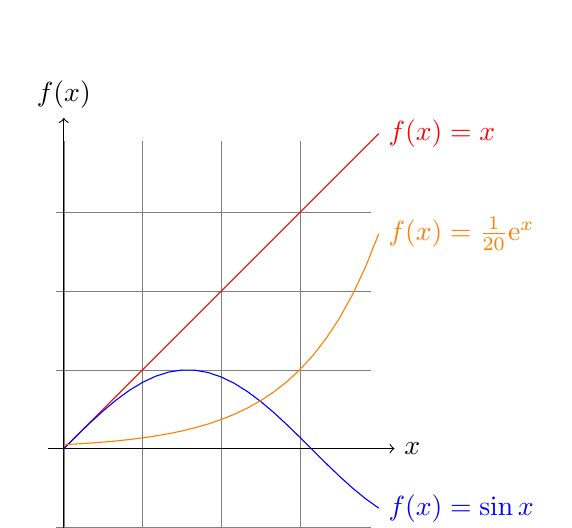
\begin{tikzpicture}[domain=0:4]
		  \draw[very thin,color=gray] (-0.1,-1.1) grid (3.9,3.9);
  		\draw[->] (-0.2,0) -- (4.2,0) node[right] {$x$};
		  \draw[->] (0,-1.2) -- (0,4.2) node[above] {$f(x)$};
		  \draw[color=red]    plot (\x,\x)             node[right] {$f(x) =x$};
  % \x r 表示弧度
		  \draw[color=blue]   plot (\x,{sin(\x r)})    node[right] {$f(x) = \sin x$};
		  \draw[color=orange] plot (\x,{0.05*exp(\x)}) node[right] {$f(x) = \frac{1}{20} \mathrm e^x$};
		\end{tikzpicture}
	%\end{center}
\end{minipage}



\begin{minipage}[htpb][80mm][t]{80mm}
	%\begin{center}
		\vspace*{60mm}
    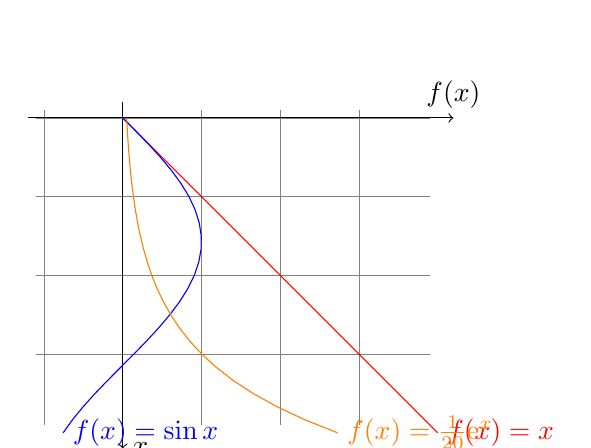
\begin{tikzpicture}[domain=0:4,scale=1,rotate=270]
		  \draw[very thin,color=gray] (-0.1,-1.1) grid (3.9,3.9);
  		\draw[->] (-0.2,0) -- (4.2,0) node[right] {$x$};
		  \draw[->] (0,-1.2) -- (0,4.2) node[above] {$f(x)$};
		  \draw[color=red]    plot (\x,\x)             node[right] {$f(x) =x$};
  % \x r 表示弧度
		  \draw[color=blue]   plot (\x,{sin(\x r)})    node[right] {$f(x) = \sin x$};
		  \draw[color=orange] plot (\x,{0.05*exp(\x)}) node[right] {$f(x) = \frac{1}{20} \mathrm e^x$};
		\end{tikzpicture}
	%\end{center}
\end{minipage}

% \chapter{公式測試}

\vskip 20 mm
\begin{minipage}[htpb]{80mm}
		\vspace*{45mm}
	%\begin{center}
			{\normalsize With normalsize 10 pt in class (truely 9.13\,pt in real dimen):
				\[ \sampleEq \]\par}

			{\Large With Large 14 pt in class (truely 12.782\,pt in real dimen):
				\[ \sampleEq \]\par}

			{\footnotesize With footnotesize 8 pt in class (truely 7.304\,pt in real dimen):
				\[ \sampleEq \]\par}
	%\end{center}
\end{minipage}

\clearpage
\begin{minipage}[htpb]{120mm}
		\vspace*{10mm}
	%\begin{center}
			{\normalsize 
				\[ \sampleEq \]\par}

			{\Large 
				\[ \sampleEq \]\par}

			{\footnotesize
				\[ \sampleEq \]\par}
	%\end{center}
\end{minipage}
% \end{withgezhu}
%\restoregeometry
\end{document}